\documentclass{article} % default font size is 10pt
\usepackage{latexsym}
\usepackage{amsfonts}
\usepackage[bbgreekl]{mathbbol}
\usepackage{amssymb}
\usepackage{amsmath}
\usepackage{amsthm}
\usepackage{amscd}
\usepackage{longtable}
\usepackage{array}
\usepackage{graphicx}
\usepackage{eucal}
\usepackage{pstricks}
\usepackage{pst-grad}
\usepackage{pst-arrow}
\usepackage{pstricks-add}
\usepackage{pst-node}
\usepackage{pst-plot}
\definecolor{antiquewhite}{rgb}{0.98, 0.92, 0.84}
\definecolor{myblue}{HTML}{15399A}
\definecolor{myred}{HTML}{B31333}
\definecolor{mygreen}{HTML}{118A4F}
\definecolor{myorange}{HTML}{DE6C06}
\definecolor{myyellow}{HTML}{E3AD30}
\definecolor{myblack}{HTML}{000000}
\definecolor{cblue}{HTML}{15399A}
\definecolor{corange}{HTML}{DE6C06}
\definecolor{myviolet}{HTML}{8601AF}
\usepackage[
backend=biber,
style=numeric,
% citestyle=alphabetic,
doi=false,
isbn=false,
url=false,
% language=false
maxcitenames=4, mincitenames=4,
maxbibnames=99, minbibnames=99
]{biblatex}
\addbibresource{action_op_ref.bib}
\usepackage{geometry}
\geometry{margin=1.5in}
\usepackage{multicol}
% QQQ Uncomment later up to line 24
% \usepackage[refpage, notintoc]{nomencl}
% \renewcommand{\nomname}{}
% \renewcommand*{\pagedeclaration}[1]{\,\,\,\hyperpage{#1}}
% \makenomenclature
% \makeindex
\usepackage{etoolbox}
% \renewcommand\nomgroup[1]{%
%   \item[\bfseries
%   \ifstrequal{#1}{C}{\addcontentsline{toc}{section}{Catalogue of Categories}  \rule[2pt]{0.45\linewidth}{1pt} Catalogue of Categories  \rule[2pt]{0.45\linewidth}{1pt}}{%
%   \ifstrequal{#1}{N}{\addcontentsline{toc}{section}{Glossary of Notation} \rule[2pt]{0.45\linewidth}{1pt} Glossary of Notation  \rule[2pt]{0.45\linewidth}{1pt}}{}}%
% ]}
\usepackage[all]{xy}
\SelectTips{cm}{11}
\UseTips
\usepackage{tikz}
\usetikzlibrary{decorations.markings,decorations.pathmorphing, arrows, calc}
\usepackage{tikz-cd}
% \usepackage{quiver}
%\tikzset{/tikz/commutative diagrams/arrow style=math font} % matching arrowheads
% \tikzset{/tikz/commutative diagrams/arrow style=tikz,>=stealth} %almost matching arrowheads; look better in pdf
\tikzset{mm/.style={execute at begin node=$\displaystyle, execute at end node=$}}
\tikzset{curve/.style={settings={#1},to path={(\tikztostart)
    .. controls ($(\tikztostart)!\pv{pos}!(\tikztotarget)!\pv{height}!270:(\tikztotarget)$)
    and ($(\tikztostart)!1-\pv{pos}!(\tikztotarget)!\pv{height}!270:(\tikztotarget)$)
    .. (\tikztotarget)\tikztonodes}},
    settings/.code={\tikzset{quiver/.cd,#1}
        \def\pv##1{\pgfkeysvalueof{/tikz/quiver/##1}}},
    quiver/.cd,pos/.initial=0.35,height/.initial=0}
\tikzset{tikzob/.style={commutative diagrams/every diagram, every cell}}
\tikzset{tikzar/.style={commutative diagrams/.cd, every arrow, every label, font={\small}}}
\tikzset{tikzsquiggle/.style={decorate, decoration={
    snake,
    segment length=8pt,
    amplitude=.9pt,post=lineto,
    post length=2pt}}}
\tikzset{cross line/.style={preaction={draw=white, -, line width=6pt}}}
\usepackage{pdfsync}
\usepackage{relsize}
\usepackage[unicode=true, pdfusetitle,
 bookmarks=true,bookmarksnumbered=false,
 breaklinks=false,
 backref=false,
 colorlinks=true,
 %linkcolor=blue!70!black,
 citecolor=black,
 urlcolor=blue!78!red,
 final
]{hyperref}
\usepackage[capitalise]{cleveref}
\newcommand{\fref}{\cref}
\newcommand{\Fref}{\Cref}
\newcommand{\prettyref}{\cref}
\newcommand{\newrefformat}[2]{}
\newcommand{\bs}{\boldsymbol}
\newcommand{\mb}{\mathbf}
\renewcommand{\dot}{\centerdot}
\renewcommand{\hat}{\widehat}
\newcommand{\R}{\mathbb{R}}
\newcommand{\ZZ}{\mathbb{Z}}
\newcommand{\N}{\mathbb{N}}
\newcommand{\m}[1]{\mathcal{#1}}
\newcommand{\id}{\textrm{id}}
\newcommand{\un}{\underline}
% \usepackage{natbib}
\renewcommand{\SS}{\mathcal{S}}
\newcommand{\colim}{\textrm{colim }}
\newcommand{\und}[1]{\ensuremath{\underline{#1}}}
\newcommand{\f}[1]{\ensuremath{\mathcal{#1}}}
\newcommand{\g}[1]{\ensuremath{\mathbb{#1}}}
\newcommand{\Cat}{\ensuremath{\textrm{Cat}}}
\newcommand{\cd}[2][]{\vcenter{\hbox{\xymatrix#1{#2}}}}
\newcommand{\Set}{\mb{Set}}
\newcommand{\twocat}{\ensuremath{$2$\textrm{-Cat}}}
\newcommand{\Icon}{\ensuremath{\textrm{Icon}}}
\newcommand{\ML}{\mathbf{\Lambda}}
\newcommand{\MLn}{\mathbf{\Lambda}_n}
\newcommand{\lop}{\Lambda^{\oplus}}
\newcommand{\MorLn}{\mathrm{Mor}(L_n)}
\newcommand{\LL}{\Lambda}
%\newcommand{\to}{\rightarrow}
\def\srarrow{\relbar\joinrel\mapstochar\joinrel\rightarrow}
%\newcommand{\id}{\ensuremath{\textnormal{id}}\xspace}
%\pdfshift
\newcommand{\quotient}[2]{ \raisebox{0.5\height}{$#1$} \mkern-5mu\diagup\mkern-4mu \raisebox{-0.5\height}{$#2$} }
\newcommand{\bigquotient}[2]{ \raisebox{0.75\height}{$#1$} \mkern-12mu\scalebox{2}{$\diagup$}\mkern-10mu \raisebox{-0.5\height}{$#2$} }
\newcommand{\pullback}{\mathbin{\text{\rotatebox{45}{$\mathlarger{\mathlarger{\mathlarger{\mathlarger{\llcorner}}}}$}}}}
\newcommand{\pushout}{\mathbin{\text{\rotatebox{225}{$\mathlarger{\mathlarger{\mathlarger{\mathlarger{\llcorner}}}}$}}}}
\newcommand{\downsim}{\rotatebox{90}{$\sim$}}
\newcommand{\EL}{E\Lambda}
\newcommand{\ELn}{E\Lambda(\underline{n})}
\newcommand{\ELnn}{E\Lambda(\underline{2n})}
\newcommand{\ELnnnn}{E\Lambda(\underline{4n})}
\newcommand{\qsn}{Q\Sigma(\underline{n})}
\newcommand{\ob}{\operatorname{Ob}}
\newcommand{\lmc}{\Lambda\mbox{-}\mb{MonCat}}
\newcommand{\sets}{\Set}
\newcommand{\mon}{\ensuremath{\mb{Mon}}}
\newcommand{\cmon}{\ensuremath{\mb{CommMon}}}
\newcommand{\moncat}{\ensuremath{\mb{MonCat}}}
\newcommand{\cat}{\ensuremath{\mb{Cat}}}
\newcommand{\epz}{\varepsilon}
\newcommand{\Alg}{\mbox{-}\mb{Alg}}
\newcolumntype{L}{>{$}l<{$}}
\newcolumntype{C}{>{$}c<{$}}
\newcolumntype{R}{>{$}r<{$}}
\newcommand{\ab}{\mathrm{ab}}
\newcommand{\gp}{\mathrm{gp}}
\newcommand{\trans}[2]{( #1 \, \, #2 )}
% \newcommand{\coeq}[4]{\left[#1;#2\right]_{#3(#4)}}
\newcommand{\coeq}[4]{#1(#4) \otimes_{#3(#4)} #2^{#4}}
\newcommand{\coequ}[4]{#1(#4) \otimes_{#3(#4)} #2_{#4}}
% \newcommand{\coequ}[4]{\left[#1;#2\right]_{#3(#4)}}
\newcommand{\coeqb}[3]{#1 \otimes_#3 #2}
\newcommand{\coeqsig}[3]{#1(#3) \otimes_{\Sigma_#3} #2^#3}
% \begin{itemize}
%   \item $P(n) \times_{\Lambda(n)} X^n$
%   \item $P(n) \bullet_{\Lambda(n)} X^n$
%   \item $P(n) ;_{\Lambda(n)} X^n$
%   \item $(P;X)_{\Lambda(n)}$
%   \item $(P \times X)^n_\Lambda$
%   \item $\left[P;X\right]_{\Lambda(n)}$
%   \item $\left[P(n);X^n\right]_{\Lambda}$
%   \item $\left[P;_{\Lambda(n)}X\right]$
%   \item $\left[P;X\right]_{\Lambda_n}$
% \end{itemize}

\crefname{lem}{Lemma}{Lemmas}
\crefname{thm}{Theorem}{Theorems}
\crefname{Defi}{Definition}{Definitions}
\crefname{nota}{Notation}{Notations}
\crefname{construction}{Construction}{Constructions}
\crefname{prop}{Proposition}{Propositions}
\crefname{rem}{Remark}{Remarks}
\crefname{remark}{Remark}{Remarks}
\crefname{cor}{Corollary}{Corollaries}
\crefname{scholium}{Scholium}{Scholia}
\crefname{figure}{Figure}{Figures}
\crefname{equation}{Equation}{Equations}
\crefname{eq}{Equation}{Equations}
\crefname{eqn}{Equation}{Equations}

\newenvironment{eq}{\begin{equation}}{\end{equation}}
\newenvironment{eqn}{\begin{equation}}{\end{equation}}
\newenvironment{eq*}{\begin{equation*}}{\end{equation*}}
\newenvironment{eqn*}{\begin{equation*}}{\end{equation*}}
\tikzset{->-/.style={decoration={markings,mark=at position #1 with {\arrow{>}}},postaction={decorate}}} 

\pgfdeclarelayer{bg}
\pgfsetlayers{bg,main}

% \numberwithin{section}{chapter}

\newtheorem{thm}{Theorem}[section]
\newtheorem{prop}[thm]{Proposition}
\newtheorem{lem}[thm]{Lemma}
\newtheorem{cor}[thm]{Corollary}
% \newtheorem{conv}[thm]

\newtheoremstyle{example}{\topsep}{\topsep}%
     {}%         Body font
     {}%         Indent amount (empty = no indent, \parindent = para indent)
     {\bfseries}% Thm head font
     {.}%        Punctuation after thm head
     {2pt}%     Space after thm head (\newline = linebreak)
     {\thmname{#1}\thmnumber{ #2}\thmnote{ #3}}%         Thm head spec
  \theoremstyle{example}
  \newtheorem{conv}[thm]{Conventions}
  \newtheorem{nota}[thm]{Notation}
  \newtheorem{example}[thm]{Example}
  \newtheorem{Defi}[thm]{Definition}
  \newtheorem{rem}[thm]{Remark}
  \newtheorem{remark}[thm]{Remark}   
    



   \title{Operads and equivariance}

% \author{Alexander S. Corner}
% % \address{}
% % \email{alex.corner@shu.ac.uk}
% \author{Nick Gurski}
% % \address{}
% % \email{nick.gurski@case.edu}
% \author{Edward Prior}
% \address{}
% \email{}
% \keywords{}
% \subjclass{}
\author{
  Alexander S. Corner\\
  \texttt{alex.corner@shu.ac.uk}
  \and
  Nick Gurski\\
  \texttt{nick.gurski@case.edu}
}
\date{}

\newcounter{artpart}
\renewcommand{\theartpart}{\Roman{artpart}}
\newcommand{\artpart}[1]{%
  \refstepcounter{artpart}%
  \addtocontents{toc}{\smallskip}%
   \addtocontents{toc}{
    \protect\contentsline{section}{
       \protect\numberline{}{\large Part \theartpart: #1}
     }{}{}
  }
  % \addtocontents{toc}{\SkipTocEntry}
  \section*{Part \theartpart: #1}}

\begin{document}


\maketitle

\tableofcontents

\abstract


%!TEX root = ../operads_paper.tex
\section{Introduction}
QQQ Needs an intro. Might be something salvageable from the original papers.

Original paper intro:

Operads were defined by May \cite{maygeom} in the early 70's to provide a convenient tool to approach problems in algebraic topology, notably the question of when a space $X$ admits an $n$-fold delooping $Y$ so that $X \simeq \Omega^{n}Y$.  An operad, like an algebraic theory \cite{lawvere-thesis}, is something like a presentation for a monad or algebraic structure.  The theory of operads has seen great success, and we would like to highlight two reasons.  First, operads can be defined in any suitable symmetric monoidal category, so that there are operads of topological spaces, of chain complexes, of simplicial sets, and of categories, to name a few examples.  Moreover, symmetric (lax) monoidal functors carry operads to operads, so we can use operads in one category to understand objects in another via transport by such a functor.  Second, operads in a fixed category are highly flexible tools.  In particular, the categories listed above all have some inherent notion of ``homotopy equivalence'' which is weaker than that of isomorphism, so we can study operads which are equivalent but not isomorphic.  These tend to have algebras which have similar features in an ``up-to-homotopy'' sense but very different combinatorial or geometric properties arising from the fact that different objects make up these equivalent but not isomorphic operads.

Operads in the category $\mb{Cat}$ of small categories have a unique flavor arising from the fact that $\mb{Cat}$ is not just a category but a 2-category.  These 2-categorical aspects have not been widely treated in the literature, although a few examples can be found.  Lack \cite{lack-cod} mentions braided $\mb{Cat}$-operads (the reader new to braided operads should refer to the work of Fiedorowicz \cite{fie-br}) in his work on coherence for 2-monads, and Batanin \cite{bat-eh} uses lax morphisms of operads in $\mb{Cat}$ in order to define the notion of an internal operad.  But aside from a few appearances, the basic theory of operads in $\mb{Cat}$ and their 2-categorical properties seems missing.  This paper was partly motivated by the need for such a theory to be explained from the ground up.

There were two additional motivations for the work in this paper.  In thinking about coherence for monoidal functors, the first author was led to a general study of algebras for multicategories internal to $\mb{Cat}$.  These give rise to 2-monads (or perhaps pseudomonads, depending on how the theory is set up), and checking abstract properties of these 2-monads prompts one to consider the simpler case of operads in $\mb{Cat}$ instead of multicategories.  The other motivation was from the second author's attempt to understand the interplay between operads in $\mb{Cat}$, operads in $\mb{Top}$, and the passage from (bi)permutative categories to $E_{\infty}$ (ring) spaces.  The first of these motivations raised the issue of when operads in $\mb{Cat}$ are cartesian, while the second led us to consider when an operad in $\mb{Cat}$ possesses a pseudo-commutative structure.

While considering how to best tackle a general discussion of operads in $\mb{Cat}$, it became clear that restricting attention to the two most commonly used types of operads, symmetric and non-symmetric operads, was both short-sighted and unnecessary.  Many theorems apply to both kinds of operads at once, with the difference in proofs being negligible; in fact, most of the arguments which applied to the symmetric case seemed to apply to the case of braided operads as well.   This led us to the notion of an action operad $\mb{G}$, and then to a definition of $\mb{G}$-operads.  In essence, this is merely the general notion of what it means for an operad $P = \{ P(n) \}_{n \in \N}$ to have groups of equivariance $\mb{G} = \{ G(n) \}_{n \in \N}$ such that $G(n)$ acts on $P(n)$.  Choosing different natural families of groups $\mb{G}$, we recover known variants of the definition of operad. \\ \begin{center}
\begin{tabular}{c|c}
Groups $\mb{G}$ & Type of operad  \\ \hline
Terminal groups & Non-symmetric operad \\
Symmetric groups & Symmetric operad \\
Braid groups & Braided operad \\
\end{tabular} \\ \end{center}
These definitions have appeared, with minor variations, in two sources of which we are aware.  In Wahl's thesis \cite{wahl-thesis}, the essential definitions appear but not in complete generality as she requires a surjectivity condition.  Zhang \cite{zhang-grp} also studies these notions\footnote{Zhang calls our action operad a \textit{group operad}.  We dislike this terminology as it seems to imply that we are dealing with an operad in the category of groups, which is not the case unless all of the maps $\pi_{n}:G(n) \rightarrow \Sigma_{n}$ are zero maps.}, once again in the context of homotopy theory, but requires the  superfluous condition that $e_{1} = \textrm{id}$ (see Lemma \ref{calclem}).

This paper consists of the following.  In Section 1, we give the definition of an action operad $\mb{G}$ and a $\mb{G}$-operad.  We develop this definition abstractly so as to apply it in any suitable symmetric monoidal category.   It is standard to express operads as monoids in a particular functor category using a composition tensor product.  In order to show that our $\mb{G}$-operads fit into this philosophy, we must work abstractly and use the calculus of coends together with the Day convolution product \cite{day-thesis}.  The reader uninterested in these details can happily skip them, although we find the route taken here to be quite satisfactory in justifying the axioms for an action operad $\mb{G}$ and the accompanying notion of $\mb{G}$-operad.  Many of our calculations are generalizations of those appearing in work of Kelly \cite{kelly-op}, although there are slight differences in flavor between the two treatments.
%Kelly:  On the operads of JP May

Section 2 works through the basic 2-categorical aspects of operads in $\mb{Cat}$.  We explain how every operad gives rise to a 2-monad, and show that all of the various 1-cells between algebras of the associated 2-monad correspond to the obvious sorts of 1-cells one might define between algebras over an operad in $\mb{Cat}$.  Similarly, we show that the algebra 2-cells, using the 2-monadic approach, correspond to the obvious notion of transformation one would define using the operad.

Section 3 studies three basic 2-categorical properties of an operad, namely the property of being finitary, the property of being 2-cartesian, and the coherence property.  The first of these always holds, as a simple calculation shows.  The second of these turns out to be equivalent to the action of $G(n)$ on $P(n)$ being free for all $n$, at least up to a certain kernel.  In particular, our characterization clearly shows that every non-symmetric operad is 2-cartesian, and that a symmetric operad is 2-cartesian if and only if the symmetric group actions are all free.  (It is useful to note that a 2-monad on $\mb{Cat}$ is 2-cartesian if and only if the underlying monad on the category of small categories is cartesian in the usual sense as the (strict) 2-pullback of a diagram is the same as its pullback.)  The third property is also easily shown to hold for any $\mb{G}$-operad on $\mb{Cat}$ using a factorization system argument due to Power \cite{power-gen}.

Section 4 then goes on to study the question of when a $\mb{G}$-operad $P$ admits a pseudo-commutative structure.  Such a structure provides the 2-category of algebras with a richer structure that includes well-behaved notions of tensor product, internal hom, and multilinear map that fit together much as the analogous notions do in the category of vector spaces.  When $P$ is contractible (i.e., each $P(n)$ is equivalent to the terminal category), this structure can be obtained from a collection of elements $t_{m,n} \in G(mn)$ satisfying certain properties.  In particular, we show that every contractible symmetric operad is pseudo-commutative, and we prove that there exist such elements $t_{m,n} \in Br_{mn}$ so that every contractible braided operad is pseudo-commutative as well (in fact in two canonical ways).  Thus Section 4 can be seen as a continuation, in the operadic context, of the work in \cite{HP}, and in particular the ``geometric'' proof of the existence of a pseudo-commutative structure for braided strict monoidal categories demonstrates the power of being able to change the groups of equivariance.

The authors would like to thank John Bourke, Martin Hyland, Tom Leinster, and Peter May for various conversations which led to this paper.  While conducting this research, the second author was supported by an EPSRC Early Career Fellowship. 

Original Borel intro:


Categories of interest are often monoidal: sets, topological spaces, and vector spaces are all symmetric monoidal, while the category of finite ordinals (under ordinal sum) is merely monoidal.  But other categories have more exotic monoidal structures.  The first such type of structure discovered was that of a braided monoidal category.  These arise in categories whose morphisms have a geometric flavor like cobordisms embedded in some ambient space \cite{js}, in  categories produced from double loop spaces \cite{fie-br}, and categories of representations over objects like quasitriangular (or braided) bialgebras \cite{street-quantum} .  Another such exotic monoidal structure is that of a coboundary category, arising in examples from the representation theory of quantum groups \cite{drin-quasihopf}.

Going back to the original work of May on iterated loop spaces \cite{maygeom}, operads were defined in both symmetric and nonsymmetric varieties.  But Fiedorowicz's work on double loop spaces \cite{fie-br} showed that there was utility in considering another kind of operad, this time with braid group actions instead of symmetric group actions.  There is a clear parallel between these definitions of different types of operads and the definitions of different kinds of monoidal category, with each given by some general schema in which varying an $\mathbb{N}$-indexed collection of groups produced the types of operads or monoidal categories seen in nature.  Building on the work in \cite{cg}, the goal of this paper is to show that this parallel can be upgraded from an intuition to precise mathematics using the notion of action operad.

An action operad $\mb{\Lambda}$ is an operad which incorporates all of the essential features of the operad of symmetric groups.  Thus $\Lambda(n)$ is no longer just a set, but instead also has a group structure together with a map $\pi_{n}:\Lambda(n) \to \Sigma_{n}$.  Operadic composition then satisfies an additional equivariance condition using the maps $\pi_n$ and the group structures.  Each action operad $\mb{\Lambda}$ produces a notion of $\mb{\Lambda}$-operad which encodes equivariance conditions using both the groups $\Lambda(n)$ and the maps $\pi_n$.  Examples include the symmetric groups, the terminal groups (giving nonsymmetric operads), the braid groups (giving braided operads), and the $n$-fruit cactus groups \cite{hk-cobound} (giving a new notion of operad one might call cactus operads).  Using a formula resembling the classical Borel construction for spaces with a group action, we can produce from any action operad $\mb{\Lambda}$ a notion of $\mb{\Lambda}$-monoidal category, in which the group $\Lambda(n)$ acts naturally on $n$-fold tensor powers of any object.  Thus the categorical Borel construction embeds action operads into a category of monads on $\mb{Cat}$, and we characterize the image of this embedding as those monads describing monoidal structures of a precise kind.

The paper is organized into the following sections.  Section 1 reviews the definition of an action operad, and defines the categorical Borel construction on them.  The key result, which reappears in proofs throughout the paper, is \cref{thm:charAOp}, characterizing action operads in terms of two new operations mimicking the block sum of permutations and the operation which takes a permutation of $n$ letters and produces a new permutation on $k_1 + k_2 + \cdots + k_n$ letters by permuting the blocks of $k_i$ letters.  In Section 2, we use this characterization and Kelly's theory of clubs \cite{kelly_club1, kelly_club0, kelly_club2} to embed action operads into monads on $\mb{Cat}$ and determine the essential image of this embedding.  Section 3 gives a construction of the free action operad from a suitable collection of data, and relates this to how clubs can be described using generators and relations.  The results of Sections 2 and 3 show that the definitions of symmetric monoidal category or coboundary category, for example, correspond to the action operad constructed from the corresponding free symmetric monoidal or coboundary category on one object; these and other examples appear in detail in Section 4.  Section 5 then extends the definition of $\mb{\Lambda}$-operad to that of $\mb{\Lambda}$-multicategory and shows that these arise abstractly via a Kleisli construction.

Copied from text:
Yau \cite{yau_infinity_2021} collects together a large number of results on the topic of action operads while also investigating the setting of infinity group operads. 

This research was supported by EPSRC 134023.

Further acknowledgements:
Alex needs to thank the LMS for a Research Reboot grant. Anybody else we've talked to about these things since their inception? Angelica? Niles? Dan Graves. Nathaniel Arkor.




\section{Notation and Conventions}\label{sec:notation}

\begin{nota}[(Symmetric groups)]\label{nota:symm_sigma}
We denote the symmetric group on the symbols $1, 2, \ldots, n$ by $\Sigma_n$. Elements of a symmetric group are usually denoted by lowercase Greek letters or written in cycle notation.
\end{nota}

\begin{nota}[(Braid groups)]\label{nota:braid}
We denote the braid group on $n$ strands by $B_n$.
\end{nota}

\begin{nota}[(Identity elements)]\label{nota:e_identity}
The symbol $e$ will generically represent an identity element in a group. If we are considering a set of groups $\{ \Lambda(n) \}_{n \in \N}$ indexed by the natural numbers, then $e_{n}$ is the identity element in $\Lambda(n)$. We will often drop the subscripts and just write $e$ when the index $n$ in $\Lambda(n)$ is either clear from context or unimportant to the argument at hand.
\end{nota}

\begin{conv}[(Identity morphisms)]\label{conv:1_id}
We generically write an identity morphism $A \to A$ as either $1$ or $1_A$.
\end{conv}

\begin{nota}[(Group actions)]\label{nota:g-action}
For a group $G$, a right $G$-action on a set $X$ will be denoted $(x,g) \mapsto x \cdot g$ or $(x,g) \mapsto x g$. 
Similar notation will be used for left actions, and for multiplication in a group.
\end{nota}

\begin{conv}[(Indexed objects)]\label{conv:indexed}
We generically write $\{ \Lambda(n) \}_{n \in \N}$ for a $\N$-indexed family of objects $\Lambda(n)$. We will occasionallywrite $\Lambda_n$ in place of $\Lambda(n)$, especially in diagrams or when the objects $\Lambda_n$ have been independently defined, as in \cref{nota:symm_sigma,nota:braid}.
\end{conv}

\begin{conv}[(Products and quotients)]\label{conv:coeq}
We will often be interested in elements of a product of the form
\[
A \times B(1) \times \cdots \times B(n) \times C
\]
(or similar, for example without $C$). We will write elements of this set as $(a; b_{1}, \ldots, b_{n}; c)$, where $b_i \in B(i)$. 
In the case that we need to consider equivalence classes of such elements, these classes will be written as $[a; b_{1}, \ldots, b_{n}; c]$. 
The most common situation in which we consider such equivalence classes is that of a coequalizer of left and right group actions in the following sense. 
A coequalizer of maps
    \[
        \xy
            (0,0)*+{A \times G \times B}="00";
            (30,0)*+{A \times B}="10";
            (60,0)*+{\coeqb{A}{B}{G}}="20";
            {\ar@<1ex>^{1 \times \lambda} "00" ; "10"};
            {\ar@<-1ex>_{\rho \times 1} "00" ; "10"};
            {\ar^{\varepsilon} "10" ; "20"};
        \endxy
    \]
will be written as $\coeqb{A}{B}{G}$, where $\rho$ is a right action of $G$ on $A$ and $\lambda$ is a left action of $G$ on $B$. 
This notation is meant to emphasize the analogy with tensor products of $R$-modules, even when the monoidal structure involved is cartesian.
It also differentiates these coequalizers from pullbacks.
\end{conv}


\begin{conv}[(Pullbacks)]\label{conv:pb}
The pullback of the diagram
    \[
        \xy
            (10,0)*+{X}="00";
            (0,-10)*+{Y}="10";
            (10,-10)*+{A}="20";
            {\ar^{f} "00" ; "20"};
            {\ar_{g} "10" ; "20"};
        \endxy
    \]
will be written as $X \times_A Y$. 
\end{conv}

\begin{Defi}](Underlying permutation)]\label{Defi:underlying-perm}
Suppose that $f \colon G \to \Sigma_n$ is a given group homomorphism, and $x \in G$. The \emph{underlying permutation} of $x$ is the element $f(x) \in \Sigma_n$. If there is likely to be some confusion as to which homomorphism $f$ is being used, we will call $f(x)$ the \emph{underlying permutation with respect to $f$}.
\end{Defi}

\begin{nota}[(Applying underlying permutations)]\label{nota:perm_shorthand}
Throughout we will be using maps $\pi_n \colon O(n) \rightarrow \Sigma_n$, where $O(n)$ is the set of $n$-ary operations of an operad $O$ and $\Sigma_n$ is the symmetric group on $n$ elements.  
For any $\sigma \in O(n)$, we will write $\sigma(i)$ for $\pi_n(\sigma)(i)$, the image of $i$ with respect to the underlying permutation of $\sigma$; the notation $\sigma^{-1}(i)$ will be used for the inverse image of $i$ with respect to the underlying permutation of $\sigma$.
\end{nota}



\begin{Defi}[(Block sum)]\label{Defi:beta-s}
Let $k_1, \ldots, k_n$ be natural numbers and suppose that $\sigma_i \in \Sigma_{k_i}$ are permutations. The \emph{block sum} of $\sigma_1, \ldots, \sigma_n$, written 
\[
\beta( \sigma_1, \ldots, \sigma_n ),
\]
is the permutation in $\Sigma_K$, where $K = \sum_{i=1}^n k_i$, given as described below. 
For $1 \leq j \leq K$, define $c$ to be the unique integer such that
\[
k_1 + \cdots + k_c < j \leq k_1 + \cdots + k_c +k_{c+1}.
\]
Define
\[
\beta( \sigma_1, \ldots, \sigma_n )(j) = k_1 + \cdots + k_c + \sigma_{c+1}\big( j - (\sum_{i=1}^c k_i) \big).
\]
\end{Defi}

\begin{rem}\label{rem:beta-s}
The formula above expresses the idea that $\beta( \sigma_1, \ldots, \sigma_n )$ permutes the first $k_1$ elements using $\sigma_1$, the next $k_2$ elements using $\sigma_2$, and so on.
\end{rem}

\begin{Defi}[(Duplication)]\label{Defi:delta-s}
Let $k_1, \ldots, k_n$ be natural numbers, and suppose that $\sigma \in \Sigma_n$ is a permutation. The \emph{duplication} of $\sigma$ with respect to $k_1, \ldots, k_n$, written
\[
\delta_{n; k_1, \ldots, k_n}(\sigma),
\]
is the permutation in $\Sigma_K$, where $K = \sum_{i=1}^n k_i$, given as described below. 
For $1 \leq j \leq K$, define $c$ to be the unique integer such that
\[
k_1 + \cdots + k_c < j \leq k_1 + \cdots + k_c +k_{c+1}.
\]
Define
\[
\delta_{n; k_1, \ldots, k_n}(\sigma)(j) = \big( \sum_{\sigma(k_i) < \sigma(k_{c+1})} k_i\big) + j - \big( \sum_{i=1}^c k_i \big).
\]
\end{Defi}

\begin{rem}\label{rem:delta-s}
The formula above for $\delta_{n; k_1, \ldots, k_n}(\sigma)$ is best explained by drawing the graph of $\sigma$ as follows. The function $\sigma$ can be represented by drawing two rows of $n$ dots each, and connecting dot $i$ in the top row to dot $\sigma(i)$ in the bottom row. Then $\delta_{n; k_1, \ldots, k_n}(\sigma)$ is obtained by 
\begin{itemize}
\item replacing dot $i$ in the top row with $k_i$ dots,
\item replacing dot $\sigma(i)$ in the bottom row with $k_i$ dots, and
\item connecting these two sets of $k_i$ dots in the unique way that preserves order.
\end{itemize}
Thus we see that the $i$th entry for $\sigma$ is duplicated $k_i$ times in $\delta_{n; k_1, \ldots, k_n}(\sigma)$.
\end{rem}

\begin{rem}\label{rem:forward-matrices}
Figure out where to put these matrices in
\cref{rem:perm_matrices}.
\end{rem}

\begin{conv}[(Superscripts)]\label{conv:superscripts}
We generically use superscripts, when needed, to distinguish between operations of the same type associated to different structures. As an example, a monoid homomorphism $f \colon A \to B$ would have axioms written as
\begin{align*}
f(x \cdot^A y) & = f(x) \cdot^B f(y), \\
f(1^A) & = 1^B.
\end{align*}
\end{conv}

%\begin{conv}\label{conv1}
%We adopt the following conventions throughout.
%\begin{enumerate}
%\item\label{conv:symm_sigma} $\Sigma_{n}$ is the symmetric group on $n$ letters, and $B_{n}$ is the braid group on $n$ strands.
%\item\label{conv:g-action} For a group $G$, a right $G$-action on a set $X$ will be denoted $(x,g) \mapsto x \cdot g$. We will use both $\cdot$ and concatenation to represent multiplication in a group.
%\item\label{conv:e_identity} The symbol $e$ will generically represent an identity element in a group. If we are considering a set of groups $\{ \Lambda(n) \}_{n \in \N}$ indexed by the natural numbers, then $e_{n}$ is the identity element in $\Lambda(n)$. We will often drop the subscripts and just write $e$ when the index $n$ in $\Lambda(n)$ is either clear from context or unimportant to the argument at hand. Occasionally we will write $\Lambda_n$ in place of $\Lambda(n)$, especially in diagrams.
%\item\label{conv:coeq} We will often be interested in elements of a product of the form
%\[
%A \times B_{1} \times \cdots \times B_{n} \times C
%\]
%(or similar, for example without $C$). We will write elements of this set as $(a; b_{1}, \ldots, b_{n}; c)$, and in the case that we need equivalence classes of such elements they will be written as $[a; b_{1}, \ldots, b_{n}; c]$. This will often be the case when we are interested in the coequalizer of left and right group actions in the following sense. A coequalizer of maps
%    \[
%        \xy
%            (0,0)*+{A \times G \times B}="00";
%            (30,0)*+{A \times B}="10";
%            (60,0)*+{\coeqb{A}{B}{G}}="20";
%            {\ar@<1ex>^{\lambda} "00" ; "10"};
%            {\ar@<-1ex>_{\rho} "00" ; "10"};
%            {\ar^{\varepsilon} "10" ; "20"};
%        \endxy
%    \]
%will be written as $\coeqb{A}{B}{G}$, where $\rho$ represents a right action of $G$ on $A$, and $\lambda$ a left action of $G$ on $B$. This is similar to the notation often used to denote pullbacks, however we find in this work that no confusion arises from using notation in this way.
%\item\label{conv:beta_delta} In the following definitions of operads, we define operad multiplication as a function
%  \[
%    \mu \colon O(n) \times O(k_1) \times \ldots O(k_n) \rightarrow O(k_1 + \ldots + k_n)
%  \]
%for each $n$, $k_1$, $\ldots$, $k_n$, and we use the following two functions as a shorthand for two commonly occuring instances of such. First we define a function
%  \[
%    \beta \colon O(k_1) \times \ldots \times O(k_n) \rightarrow O(k_1 + \ldots + k_n)
%  \]
%for each $n$, $k_1$, $\ldots$, $k_n$, which takes elements $\tau_1 \in O(k_1)$, $\ldots$, $\tau_n \in O(k_n)$ and produces the element
%  \[
%    \beta(\tau_1, \ldots, \tau_n) = \mu(e_n; \tau_1, \ldots, \tau_n).
%  \]
%We think of this element as the block sum of the elements $\tau_1$, $\ldots$, $\tau_n$. We also define a function
%  \[
%    \delta_{n;k_1,\ldots,k_n} \colon O(n) \rightarrow O(k_1 + \ldots + k_n)
%  \]
%for each $n$, $k_1$, $\ldots$, $k_n$, which takes an element $\sigma \in O(n)$ and produces the element
%  \[
%    \delta(\sigma) = \mu(\sigma;e_{k_1}, \ldots, e_{k_n}).
%  \]
%
%In the particular case of the symmetric groups, these are functions
%  \[
%    \beta \colon \Sigma_{k_1} \times \Sigma_{k_n} \rightarrow \Sigma_{k_1 + \ldots + k_n}
%  \]
%and
%  \[
%    \delta_{n;k_1,\ldots,k_n} \colon \Sigma_{n} \rightarrow \Sigma_{k_1 + \ldots + k_n}.
%  \]
%In the case of $\beta$ we form the block sum permutation $\beta(\tau_1,\ldots,\tau_n)$ which permutes the first $k_{1}$ elements according to $\tau_{1}$, the next $k_{2}$ elements according to $\tau_{2}$ and so on; this is an element of $\Sigma_{k_{1} + \cdots + k_{n}}$. For $\delta$ we take the permutation $\delta(\sigma) \in \Sigma_{k_{1} + \cdots + k_{n}}$ to be that which permutes the $n$ different blocks $1$ through $k_{1}$, $k_{1}+1$ through $k_{1} + k_{2}$, and so on, according to the permutation $\sigma \in \Sigma_{n}$. We expand on this at various points, including in \cref{rem:perm_matrices}.
%\item\label{conv:perm_shorthand} Throughout we will be using maps $\pi_n \colon O(n) \rightarrow \Sigma_n$, where $O(n)$ is the object of $n$-ary operations of an operad $O$ and $\Sigma_n$ is the symmetric group on $n$ elements. The map $\pi_n$ in each case will represent a form of `underlying permutation' of each element, which we will then use to act on operad multiplication. As the notation starts to become cumbersome, we will often write $\sigma^{-1}(i)$ which should be read as $\pi_n(\sigma)^{-1}(i)$, where $\sigma \in O(n)$.
%\item\label{conv:op_superscript} We adopt the convention that if an equation requires using operadic composition in more than one operad, we will indicate this by a superscript on each instance of $\mu$ unless it is entirely clear from context. This can be seen, for example, in \cref{Defi:op_map}.
%\end{enumerate}
%\end{conv}

\artpart{Operads and Action Operads}

\section{Background: Operads}\label{sec:back-op}

This section will collect the basic background information on operads that we will later generalize in\ngnote{ref later sections}. We begin with the most common type of operad, a symmetric operad, before defining two more types of operad: plain and braided. 

\begin{Defi}[(Symmetric operad)]\label{Defi:sym-op}
A \textit{symmetric operad} $O$ (in the category of sets) consists of
\begin{itemize}
\item a set, $O(n)$, for each natural number $n$,
\item for each $n$, a right $\Sigma_{n}$-action on $O(n)$,
\item an element $\id \in O(1)$, and
\item functions
  \[
    \mu \colon  O(n) \times O(k_{1}) \times \cdots \times O(k_{n}) \rightarrow O(k_{1} + \cdots + k_{n}),
  \]
\end{itemize}
satisfying the following three axioms.
\begin{enumerate}
\item The element $\id \in O(1)$ is a two-sided unit for $\mu$, meaning that
  \begin{align*}
    \mu(\id;x) &= x,\\
    \mu(x;\id,\ldots,\id) &= x
  \end{align*}
for any $x \in O(n)$.
\item The functions $\mu$ are associative, meaning that the diagram below commutes.
% \[
% \xy
% (0,0)*+{\scriptstyle O(n) \times O(k_{1}) \times \cdots \times O(k_{n}) \times O(l_{1,1}) \times \cdots \times O(l_{{1},k_{1}}) \times \cdots \times O(l_{n,1}) \times \cdots \times O(l_{{n},k_{n}})} ="00";
% (0,-50)*+{\scriptstyle O(k_{1} + \cdots + k_{n}) \times O(l_{1,1}) \times \cdots \times O(l_{{1},k_{1}}) \times \cdots \times O(l_{n,1})\times \cdots \times O(l_{{n},k_{n}})} ="02";
% (55,-10)*+{\scriptstyle O(n) \times \prod_{i=1}^n O(k_{i}) \times O(l_{i,1}) \times \cdots \times O(l_{{i}, k_{i}}) } ="20";
% (55,-25)*+{\scriptstyle O(n) \times O(\sum l_{1,-}) \times \cdots \times O(\sum l_{n,-})} ="21";
% (55, -40)*+{\scriptstyle  O(\sum l_{-,-})} ="22";
% {\ar_{\scriptstyle \mu \times 1} "00" ; "02"};
% {\ar_{\mu} "02" ; "22"};
% {\ar^{\cong} "00" ; "20"};
% {\ar^{1 \times \prod \mu} "20" ; "21"};
% {\ar^{\mu} "21" ; "22"};
% \endxy
% \]


  \[
    \xy
      (0,0)*+{\scriptstyle O(n) \times \left(\prod_{i=1}^n O(k_i)\right) \times \left(\prod_{i=1}^n\prod_{j=1}^{k_i} O(l_{i,j})\right)}="a";
      (65,0)*+{\scriptstyle O(n) \times \prod_{i=1}^n \left(O(k_i) \times \prod_{j=1}^{k_i} O(l_{i,j})\right)}="b";
      (65,-20)*+{\scriptstyle O(n) \times \prod_{i=1}^n O\left(\sum_{j=1}^{k_i} l_{i,j}\right)}="c";
      (65,-40)*+{\scriptstyle O\left(\sum_{i=1}^n \sum_{j=1}^{k_i} l_{i,j}\right)}="d";
      (0,-40)*+{\scriptstyle O\left(\sum_{i=1}^n k_i\right) \times \prod_{i=1}^n \prod_{j=1}^{k_i} O(l_{i,j})}="e";
      %
      {\ar^{\cong} "a" ; "b"};
      {\ar^{1 \times \prod \mu} "b" ; "c"};
      {\ar^{\mu} "c" ; "d"};
      {\ar_{\mu \times 1} "a" ; "e"};
      {\ar_{\mu} "e" ; "d"};
    \endxy
  \]

\item The functions $\mu$ are equivariant with respect to the symmetric group actions, meaning that two equations hold.
\begin{itemize}
\item[3.1] Suppose that $x \in O(n)$, $y_i \in O(k_i)$ for $i = 1, \ldots, n$, and $\tau_i \in \Sigma_{k_i}$ for  $i = 1, \ldots, n$. Then the first equivariance axiom is the requirement that
\[
\mu(x;y_1 \cdot \tau_1,\ldots,y_n \cdot \tau_n) = \mu(x;y_1,\ldots,y_n)\cdot \beta(\tau_1,\ldots,\tau_n)
\]
holds, where $\beta$ is the function from \cref{Defi:beta-s}.
\end{itemize}
\begin{itemize}
\item[3.2] Suppose that  $x \in O(n)$, $y_i \in O(k_i)$ for $i = 1, \ldots, n$, and $\sigma \in \Sigma_{n}$. 
Then the second equivariance axiom is the requirement that
\[
 \mu(x \cdot \sigma; y_1, \ldots, y_n) = \mu\left(x;y_{\sigma^{-1}(1)},\ldots,y_{\sigma^{-1}(n)}\right)\cdot \delta_{n; k_1, \ldots, k_n}(\sigma)
\]
holds, where $\delta_{n; k_1, \ldots, k_n}$ is the function from \cref{Defi:delta-s}.
\end{itemize}
%
%the following two equations hold.
%  \begin{align*}
%    \mu(x;y_1 \cdot \tau_1,\ldots,y_n \cdot \tau_n) &= \mu(x;y_1,\ldots,y_n)\cdot \beta(\tau_1,\ldots,\tau_n)\\
%    \mu(x \cdot \sigma; y_1, \ldots, y_n) &= \mu\left(x;y_{\sigma^{-1}(1)},\ldots,y_{\sigma^{-1}(n)}\right)\cdot \delta(\sigma)
%  \end{align*}
%  % \begin{align*}
%  %   \mu(x;y_1 \cdot \tau_1,\ldots,y_n \cdot \tau_n) &= \mu(x;y_1,\ldots,y_n)\cdot(\tau_1 \oplus \ldots \oplus \tau_n)\\
%  %   \mu(x \cdot \sigma; y_1, \ldots, y_n) &= \mu\left(x;y_{\sigma^{-1}(1)},\ldots,y_{\sigma_{-1}(n)}\right)\cdot \sigma^+
%  % \end{align*}
%  For the first equation above, we 
\end{enumerate}
\end{Defi}

\begin{term}[(Operadic multiplication, composition)]\label{term:operadic-mult}
The functions $\mu$ in \cref{Defi:sym-op} are called \emph{operadic multiplication} or \emph{operadic composition} maps.
\end{term}

\begin{rem}\label{rem:op-def}
One is intended to think that $x \in O(n)$ is a function with $n$ inputs and a single output, as below.
  \begin{center}
  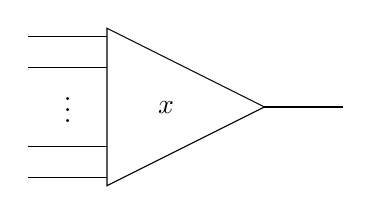
\begin{tikzpicture}
    \draw (0,0.9) -- (1,0.9);
    \draw (0,0.5) -- (1,0.5);
    %
    \node [anchor=center] () at (0.5,0) {$\vdots$\strut};
    %
    \draw (0,-0.5) -- (1,-0.5);
    \draw (0,-0.9) -- (1,-0.9);
    %
    \draw (1,1) -- (1,-1) -- (3,0) -- cycle;
    %
    \draw (3,0) -- (4,0);
    %
    \node [anchor=center] () at (1.75,0) {$x$\strut};
  \end{tikzpicture}
  \end{center}
  % \[
  %   \xy
  %     {\ar@{-} (0,0)*{}; (25,-10)*{} };
  %     {\ar@{-} (0,-20)*{}; (25,-10)*{} };
  %     {\ar@{-} (0,0)*{}; (0,-20)*{} };
  %     {\ar@{-} (25,-10)*{}; (35,-10)*{} };
  %     {\ar@{-} (0,0)*{}; (-10,0)*{} };
  %     {\ar@{-} (0,-3)*{}; (-10,-3)*{} };
  %     {\ar@{-} (0,-17)*{}; (-10,-17)*{} };
  %     {\ar@{-} (0,-20)*{}; (-10,-20)*{} };
  %     (11,-10)*{x}; (-5,-10)*{\vdots}
  %   \endxy
  % \]
Operadic composition is then a generalization of function composition, with the pictorial representation below being $\mu(x; y_{1}, y_{2})$ for $\mu \colon O(2) \times O(2) \times O(3) \rightarrow O(5)$.
  \begin{center}
  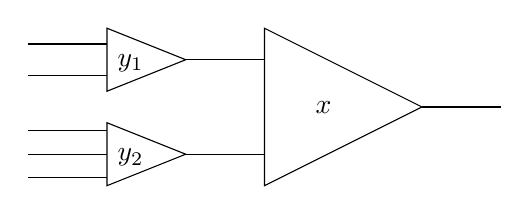
\begin{tikzpicture}
    % upper triangle
    \draw (-2,0.8) -- (-1,0.8);
    %
    \draw (-2,0.4) -- (-1,0.4);
    %
    \draw (-1,1) -- (-1,0.2) -- (0,0.6) -- cycle;
    %
    \node [anchor=center] () at (-0.7,0.6) {$y_1$\strut};    
    % lower triangle
    \draw (-2,-0.9) -- (-1,-0.9);
    %
    \draw (-2,-0.3) -- (-1,-0.3);
    %
    \draw (-1,-1) -- (-1,-0.2) -- (0,-0.6) -- cycle;
    %
    \draw (-2,-0.6) -- (-1,-0.6);
    %
    \node [anchor=center] () at (-0.7,-0.6) {$y_2$\strut};
    % big triangle
    \draw (0,0.6) -- (1,0.6);
    %    
    \draw (0,-0.6) -- (1,-0.6);
    %
    \draw (1,1) -- (1,-1) -- (3,0) -- cycle;
    %
    \draw (3,0) -- (4,0);
    %
    \node [anchor=center] () at (1.75,0) {$x$\strut};
  \end{tikzpicture}
  \end{center}
  % \[
  %   \xy
  %     {\ar@{-} (0,0)*{}; (25,-10)*{} };
  %     {\ar@{-} (0,-20)*{}; (25,-10)*{} };
  %     {\ar@{-} (0,0)*{}; (0,-20)*{} };
  %     {\ar@{-} (25,-10)*{}; (35,-10)*{} };
  %     {\ar@{-} (0,-3)*{}; (-10,-3)*{} };
  %     {\ar@{-} (0,-17)*{}; (-10,-17)*{} };
  %     (11,-10)*{x};
  %     {\ar@{-} (-25,2)*{}; (-10,-3)*{} };
  %     {\ar@{-} (-25,-8)*{}; (-10,-3)*{} };
  %     {\ar@{-} (-25,2)*{}; (-25,-8)*{} };
  %     {\ar@{-} (-25,1)*{}; (-30,1)*{} };
  %     {\ar@{-} (-30,-7)*{}; (-25,-7)*{} };
  %     (-19,-3)*{y_{1}};
  %     {\ar@{-} (-25,-12)*{}; (-10,-17)*{} };
  %     {\ar@{-} (-25,-22)*{}; (-10,-17)*{} };
  %     {\ar@{-} (-25,-12)*{}; (-25,-22)*{} };
  %     {\ar@{-} (-25,-13)*{}; (-30,-13)*{} };
  %     {\ar@{-} (-25,-17)*{}; (-30,-17)*{} };
  %     {\ar@{-} (-25,-21)*{}; (-30,-21)*{} };
  %     (-19,-17)*{y_{2}};
  %   \endxy
  % \]
  \end{rem}

\begin{term}[($n$-ary operations)]\label{term:nary-ops}
The set $O(n)$ in \cref{Defi:sym-op} is called the set of \emph{$n$-ary operations} of $O$.
\end{term}

\begin{rem}\label{rem:nary-ops-V}
If $O$ is an operad in a category other than $\mb{Sets}$ (see \cref{rem:V-and-coll}), then we would call $O(n)$ the \emph{object} of $n$-ary operations.
\end{rem}

%\begin{rem}\label{Rem:sigma_conditions}
%It is useful to write out in full what the sets in the diagram of the second axiom above mean. The use of numerous products and indices is to save space but the full picture becomes much clearer when these are expanded. For the equations in the third axiom above to make sense, we must have
%\begin{itemize}
%\item $x \in O(n)$,
%\item $y_{i} \in O(k_{i})$ for $i=1, \ldots, n$,
%\item $\tau_{i} \in \Sigma_{k_{i}}$,
%\item $\sigma \in \Sigma_{n}$, and
%\item $\beta(\tau_1,\ldots,\tau_n), \delta(\sigma) \in \Sigma_{k_1 + \ldots + k_n}$ as described in \cref{conv1} \eqref{conv:beta_delta}.
%\end{itemize}
%
%\end{rem}

Here are two important examples of symmetric operads.

\begin{example}[(Symmetric operad of symmetric groups)]\label{ex:Sigma}
The canonical example of \emph{a} symmetric operad is \emph{the} symmetric operad which we write as $\Sigma$. The set $\Sigma(n)$ is the set of elements of the symmetric group $\Sigma_{n}$, and the group action is just multiplication on the right. The identity element $\id \in \Sigma(1)$ is just the identity permutation on a one-element set. Operadic composition in $\Sigma$ will then be given by a function
  \[
    \Sigma(n) \times \Sigma(k_{1}) \times \cdots \times \Sigma(k_{n}) \rightarrow \Sigma(k_{1} + \cdots + k_{n})
  \]
which takes permutations $\sigma \in \Sigma_{n}, \tau_{i} \in \Sigma_{k_{i}}$ and produces the following permutation in $\Sigma_{k_{1} + \cdots + k_{n}}$:
  \[
    \mu(\sigma; \tau_{1}, \ldots, \tau_{n}) = \delta(\sigma) \cdot \beta(\tau_1,\ldots,\tau_n),
  \]
with $\beta$ and $\delta$ as in \cref{conv1}.

Below we have drawn the permutation for the composition
  \[
    \mu \colon \Sigma(3) \times \Sigma(2) \times \Sigma(4) \times \Sigma(3) \rightarrow \Sigma(9)
  \]
evaluated on the element $\left( (1 \,\, 2 \,\, 3); \trans{1}{2},\trans{1}{2}\trans{3}{4},\trans{1}{3} \right)$, in terms of $\beta$ and $\delta$. We expand on this in \cref{thm:charAOp}.
  \begin{center}
  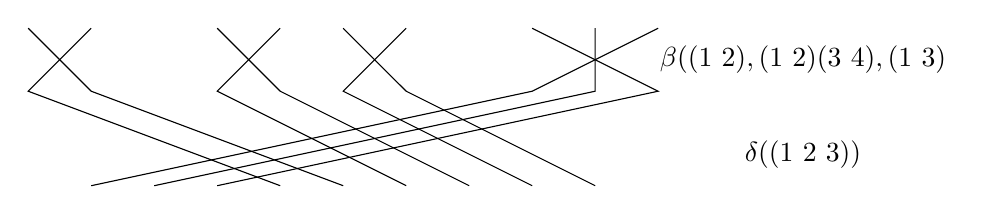
\begin{tikzpicture}[scale=0.8]
  \draw (1,0) -- (2,-1) -- (6,-2.5);
  \draw (2,0) -- (1,-1) -- (5,-2.5);
  \draw (4,0) -- (5,-1) -- (8,-2.5);
  \draw (5,0) -- (4,-1) -- (7,-2.5);
  \draw (6,0) -- (7,-1) -- (10,-2.5);
  \draw (7,0) -- (6,-1) -- (9,-2.5);
  \draw (9,0) -- (11,-1) -- (4,-2.5);
  \draw (10,0) -- (10,-1) -- (3,-2.5);
  \draw (11,0) -- (9,-1) -- (2,-2.5);
  \node at (13.3,-0.5) {$\beta(\trans{1}{2},\trans{1}{2}\trans{3}{4}, \trans{1}{3}$};
  \node at (13.3,-2) {$\delta((1 \,\, 2 \,\, 3))$};
  \end{tikzpicture}
  \end{center}
  % \[
  %   \xy
  %     {\ar@{-} (0,0)*{}; (5,-5)*{} };
  %     {\ar@{-} (5,0)*{}; (0,-5)*{} };
  %     {\ar@{-} (12,0)*{}; (17,-5)*{} };
  %     {\ar@{-} (17,0)*{}; (12,-5)*{} };
  %     {\ar@{-} (22,0)*{}; (27,-5)*{} };
  %     {\ar@{-} (27,0)*{}; (22,-5)*{} };
  %     {\ar@{-} (34,0)*{}; (44,-5)*{} };
  %     {\ar@{-} (39,0)*{}; (39,-5)*{} };
  %     {\ar@{-} (44,0)*{}; (34,-5)*{} };
  %     {\ar@{-} (0,-5)*{}; (17,-13)*{} };
  %     {\ar@{-} (5,-5)*{}; (22,-13)*{} };
  %     {\ar@{-} (12,-5)*{}; (29,-13)*{} };
  %     {\ar@{-} (17,-5)*{}; (34,-13)*{} };
  %     {\ar@{-} (22,-5)*{}; (39,-13)*{} };
  %     {\ar@{-} (27,-5)*{}; (44,-13)*{} };
  %     {\ar@{-} (34,-5)*{}; (0,-13)*{} };
  %     {\ar@{-} (39,-5)*{}; (5,-13)*{} };
  %     {\ar@{-} (44,-5)*{}; (10,-13)*{} };
  %   \endxy
  % \]
  
 \textbf{End this example here, with labels, move the rest to after 2.26.}

\begin{remark}\label{Rem:perm_matrices}
Permutations, as elements of $\Sigma_n$, can be considered as permutation \emph{matrices}, matrices with exactly one $1$ in each row and column. E.g., the permutation $(1 \,\, 3 \,\, 2) \in \Sigma_3$ can be considered as the matrix
  \[
  \begin{bmatrix}
  0 & 0 & 1 \\
  1 & 0 & 0 \\
  0 & 1 & 0
  \end{bmatrix},
  \]
which permutes three elements $  \begin{bmatrix} a & b & c \end{bmatrix}$ by pre-multiplying by the permutation matrix:
  \[
  \begin{bmatrix}
  0 & 0 & 1 \\
  1 & 0 & 0 \\
  0 & 1 & 0
  \end{bmatrix}
  \begin{bmatrix}
  a \\ b \\ c
  \end{bmatrix}
  =
  \begin{bmatrix}
  c \\ a \\ b
  \end{bmatrix}.
  \]
Then $\beta$ corresponds to the process of taking the block diagonal matrix of the original permutation matrices. So given elements $\trans{1}{2} \in \Sigma_2$, $e_1 \in \Sigma_1$, and $(1 \,\, 3 \,\, 2) \in \Sigma_3$, then
  \begin{align*}
  \beta(\trans{1}{2},e_1,(1 \,\, 2 \,\, 3)) &=
  \begin{bmatrix}
  \begin{bmatrix}
  0 & 1 \\
  1 & 0
  \end{bmatrix} & 0 & 0 \\
  0 & \begin{bmatrix} 1 \end{bmatrix} & 0 \\
  0 & 0 &   \begin{bmatrix}
  0 & 0 & 1 \\
  1 & 0 & 0 \\
  0 & 1 & 0
  \end{bmatrix}
  \end{bmatrix}\\
  &=
  \begin{bmatrix}
  0 & 1 & 0 & 0 & 0 & 0 \\
  1 & 0 & 0 & 0 & 0 & 0 \\
  0 & 0 & 1 & 0 & 0 & 0 \\
  0 & 0 & 0 & 0 & 0 & 1 \\
  0 & 0 & 0 & 1 & 0 & 0 \\
  0 & 0 & 0 & 0 & 1 & 0 \\
  \end{bmatrix} \\
  &= \trans{1}{2}(3)(4 \,\, 5 \,\, 6).
  \end{align*}
Similarly, we can describe $\delta$ as an operation on permutation matrices. The idea here is that for $\sigma \in \Sigma_n$, $\delta_{n;k_1,\ldots,k_n}(\sigma)$ takes a block diagonal of identity matrices $I_{k_1}$, $\ldots$, $I_{k_n}$ (which corresponds to $\beta(e_{k_1},\ldots,e_{k_n}) \in \Sigma_{k_1+\ldots+k_n}$), and permutes these according to the effect of the permutation $\sigma$. For example, given $\sigma = (1 \,\, 2 \,\, 3)$, then
  \[
    \delta_{3;2,1,3}(\sigma) =
    \begin{bmatrix}
    I_2 & 0 & 0 \\
    0 & I_1 & 0 \\
    0 & 0 & I_3
    \end{bmatrix}
    \ast
    \sigma
    =
      \begin{bmatrix}
      0 & 0 & 1 \\
      1 & 0 & 0 \\
      0 & 1 & 0
      \end{bmatrix}
    \ast
    \begin{bmatrix}
    I_2 & 0 & 0 \\
    0 & I_1 & 0 \\
    0 & 0 & I_3
    \end{bmatrix}
    =
    \begin{bmatrix}
    0 & 0 & I_3 \\
    I_2 & 0 & 0 \\
    0 & I_1 & 0
    \end{bmatrix}.
  \]
We make use of a similar interpretation of signed permutations and block diagonal matrices in a counterexample given in \cref{Ex:counterex}.
\end{remark}

  
Note that $(12)(34) \in \Sigma(4)$ is actually $\mu(e_{2}; (12), (12))$, where $e_{2} \in \Sigma_{2}$ is the identity permutation. Using this and operad associativity, one can easily check that
  \[
    \mu \left( (123); (12), (12)(34), (13) \right) = \mu \left( (1234); (12), (12), (12), (13) \right),
  \]
where now the composition on the right side uses the function
  \[
    \mu \colon \Sigma(4) \times \Sigma(2) \times \Sigma(2) \times \Sigma(2) \times \Sigma(3) \rightarrow \Sigma(9).
  \]
This equality is obvious using the picture above, but verifiable directly using only the algebra of the symmetric operad.
\end{example}

\begin{example}[(Endomorphism operad)]\label{ex:endo}
Let $X$ be a set. The \emph{endomorphism operad} of $X$, denoted $\mathcal{E}_X$, consists of 
\begin{itemize}
\item the sets
\[
\mathcal{E}_X(n) = \mb{Sets}(X^n, X),
\]
\item the right group actions $\mathcal{E}_X(n) \times \Sigma_n \to \mathcal{E}_X(n)$ given by
\[
(f \cdot \sigma)(x_1, \ldots, x_n) = f( x_{\sigma^{-1}(1)}, \ldots, x_{\sigma^{-1}(n)}),
\]
\item the element $\id \in \mathcal{E}_X(1)$ being the identity function $1 \colon X \to X$, and
\item operadic multiplication given by
\[
\mu(g; f_1, \ldots, f_n) = g \circ (f_1 \times \cdots \times f_n).
\]
\end{itemize}
We leave verification of the axioms to the reader, or recommend\ngnote{may-GoILS, find specific ref number}.
\end{example}

\begin{rem}
Intuition in \cref{rem:op-def} connected with example \cref{ex:endo} through the concept of an algebra, see\ngnote{later section} for these.
\end{rem}

One can also drop the symmetric group actions entirely to obtain the notion of a non-symmetric or plain operad.

\begin{Defi}[(Non-symmetric operad)]\label{Defi:non-sym-op}
A \emph{non-symmetric operad} $O$ consists of 
\begin{itemize}
\item a set, $O(n)$, for each natural number $n$,
%\item for each $n$, a right $\Sigma_{n}$-action on $O(n)$,
\item an element $\id \in O(1)$, and
\item functions
  \[
    \mu \colon  O(n) \times O(k_{1}) \times \cdots \times O(k_{n}) \rightarrow O(k_{1} + \cdots + k_{n}),
  \]
\end{itemize}
satisfying axioms 1 and 2 from \cref{Defi:sym-op}.
\end{Defi}

\begin{rem}\label{rem:V-and-coll}
\begin{enumerate}
\item One can change from operads in $\mb{Sets}$ to operads in another (symmetric) monoidal category $\mathcal{V}$ by requiring each $O(n)$ to be an object of $\mathcal{V}$ and replacing all instances of cartesian product with the appropriate tensor product in $\mathcal{V}$. One would also the element $\id \in O(1)$ with a map $I \rightarrow O(1)$ from the unit object of $\mathcal{V}$ to $O(1)$. In the case of symmetric operads, one would also express the right group actions as homomorphisms
\[
\Sigma_n^{op} \to \mathcal{V}\big( O(n), O(n) \big).
\]
\item Every symmetric operad has an underlying \textit{symmetric collection} which consists of the natural number-indexed set $\{ O(n) \}_{n \in \N}$ together with symmetric group actions, but without a chosen identity element or composition maps. The category of symmetric collections is a presheaf category, and we will equip it with a monoidal structure in which monoids are precisely operads in \cref{operad=monoid}. A similar construction, but without reference to group actions, shows that every non-symmetric operad has an underlying (non-symmetric) collection which is now merely a $\N$-indexed collection of sets.
\end{enumerate}
\end{rem}

\begin{example}\label{ex:non-sym}
\ngnoteil{insert example of non-symmetric operad here, how about Trimble's thing in dimension 1?}
\end{example}

\cref{ex:non-sym}

In the original topological applications \cite{maygeom}, symmetric operads were the central figures. A further kind of operad was studied by Fiedorowicz in \cite{fie-br}, that of a \emph{braided} operad in which the braid groups take the place of the symmetric groups. We sketch that definition below, but postpone details to\ngnote{write this out later, ref back}.

\begin{Defi}[(Braided operad, sketch)]\label{Defi:broperad}
A \textit{braided operad} consists of
  \begin{itemize}
    \item a non-symmetric operad $O$ and
    \item for each $n$, a right action of the $n$th braid group $B_{n}$ on $O(n)$,
  \end{itemize}
%satisfying the following axioms.
%  \begin{align*}
%    \mu(x;y_1 \cdot \tau_1,\ldots,y_n \cdot \tau_n) &= \mu(x;y_1,\ldots,y_n)\cdot\beta(\tau_1,\ldots,\tau_n)\\
%    \mu(x \cdot \sigma; y_1, \ldots, y_n) &= \mu\left(x;y_{\sigma^{-1}(1)},\ldots,y_{\sigma^{-1}(n)}\right)\cdot \delta_{n; k_1, \ldots, k_n}(\sigma)
%  \end{align*}
%  
such that the operadic multiplication functions $\mu$ are equivariant with respect to the braid group actions, meaning that two equations hold.
\begin{itemize}
\item[1] Suppose that $x \in O(n)$, $y_i \in O(k_i)$ for $i = 1, \ldots, n$, and $\tau_i \in B_{k_i}$ for  $i = 1, \ldots, n$. Then the first equivariance axiom is the requirement that
\[
\mu(x;y_1 \cdot \tau_1,\ldots,y_n \cdot \tau_n) = \mu(x;y_1,\ldots,y_n)\cdot \beta(\tau_1,\ldots,\tau_n)
\]
holds.%, where $\beta$ is the function from \cref{Defi:beta-s}.
\item[2] Suppose that  $x \in O(n)$, $y_i \in O(k_i)$ for $i = 1, \ldots, n$, and $\sigma \in B_{n}$. 
Then the second equivariance axiom is the requirement that
\[
 \mu(x \cdot \sigma; y_1, \ldots, y_n) = \mu\left(x;y_{\sigma^{-1}(1)},\ldots,y_{\sigma^{-1}(n)}\right)\cdot \delta_{n; k_1, \ldots, k_n}(\sigma)
\]
holds.%, where $\delta_{n; k_1, \ldots, k_n}$ is the function from \cref{Defi:delta-s}.
\end{itemize}
%For the above equations to make sense, we require similar conditions on the elements to those in \cref{rem:sigma_conditions}.
% For the above equations to make sense, we must have
%   \begin{itemize}
%       \item $x \in O(n)$,
%       \item $y_{i} \in O(k_{i})$ for $i=1, \ldots, n$,
%       \item $\tau_{i} \in B_{k_{i}}$, and
%       \item $\sigma \in B_{n}$.
%   \end{itemize}
\end{Defi}

\begin{rem}\label{rem:br-op-needed}
The above sketch omits the definitions of $\beta, \delta$ for braids. 
Formulas for these can be found in \cite[Examples~5.1.11,~5.1.13]{yau_infinity_2021}, although the geometric interpretations are simple: $\beta$ takes the disjoint union of braids, and $\delta_{n; k_1, \ldots, k_n}(\tau)$ is obtained by replacing the $i$th strand of $\tau$ by $k_i$ parallel strands.
These operations are sometimes referred to as `cabling' operations for braids, as described in, for example, \cite{doucot_local_2025}.
\end{rem}

\begin{example}\label{ex:braided-op}
\ngnoteil{insert example of braided operad here, probably just braid groups??}
\end{example}

\ngnoteil{can we prove that the operad of braid groups is NOT a symmetric operad?}

We conclude this section by defining various categories of operads in $\mb{Sets}$, although the reader can generalize these to categories of operads in any symmetric monoidal category. We focus on the case of symmetric operads, and explain after how to modify the definitions for non-symmetric or braided operads.

\begin{Defi}[(Map of symmetric operads)]\label{Defi:sym_op_map}
Let $O, O'$ be symmetric operads in $\mb{Sets}$. Then a \textit{map of symmetric operads} (or just \emph{operad map} for short, when it is clear that the intent is to respect the symmetric group actions) $f \colon O \rightarrow O'$ consists of functions $f_{n} \colon O(n) \rightarrow O'(n)$ for each natural number such that the following axioms hold for all $x \in O(n), y_i \in O(k_i), \sigma \in \Sigma_n$.

  \begin{align*}
    f\left(\id_O\right) &= \id_{O'}\\
    f\left(\mu^{O}(x;y_1,\ldots,y_n)\right) &= \mu^{O'}\left(f(x);f(y_1),\ldots,f(y_n)\right)\\
    f(x \cdot \sigma) & = f(x) \cdot \sigma
  \end{align*}
\end{Defi}

The next proposition states that symmetric operads and their maps form a category. We leave the proof to the reader.

\ngnoteil{let's use the following prop/notation pair as a template for how to define categories}
\begin{prop}\label{prop:cat-of-sym-op}
There is a category with 
\begin{itemize}
\item objects the symmetric operads $O$ in $\mb{Sets}$, 
\item morphisms the maps of symmetric operads between them,
\item identities $1_O \colon O \to O$ given by
\[
(1_O)_n = 1_{O(n)} \colon O(n) \to O(n),
\]
and
\item composition given by
\[
(g \circ f)_n = g_n \circ f_n.
\]
\end{itemize}
\end{prop}

\begin{nota}[(The category of symmetric operads)]\label{nota:cat-of-sym-op}
The category in \cref{prop:cat-of-sym-op} is called the \emph{category of symmetric operads (in $\mb{Sets}$)}, and is denoted $\Sigma\mbox{-}\mb{Op}$.
\end{nota}

\begin{rem}[(The category of non-symmetric operads)]\label{rem:cat-of-nonsym-op}

\end{rem}

\begin{rem}[(The category of braided operads)]\label{rem:cat-of-br-op}

\end{rem}

\section{Action Operads}\label{sec:aop}

The axioms for both symmetric and braided operads use the following features.
\begin{enumerate}
\item For each $n$, we have a group $\Lambda_n$ acting on the set $O(n)$ of $n$-ary operations of the operad. Each such group is equipped with a homomorphism $\pi_n \colon \Lambda_n \to \Sigma_n$, so that every element of $\Lambda_n$ has an underlying permutation.
\item The first equivariance axiom requires the additional data of a family of functions
\[
\beta \colon \Lambda_{k_1} \times \cdots \Lambda_{k_n} \to \Lambda_{k_1 + \cdots + k_n}.
\]
In order for this to be a well-defined function, the right group action axioms force these functions to be group homomorphisms.
\item The second equivariance axiom requires the additional data of a family of functions
\[
\delta_{n; k_1, \ldots, k_n} \colon \Lambda_{k_1} \times \cdots \Lambda_{k_n} \to \Lambda_{k_1 + \cdots + k_n}.
\]
These functions are not forced to be group homomorphisms, but do satisfy some additional axioms.
\end{enumerate}
In this section, we define \emph{action operads} in \cref{Defi:aop} in order to present a unified treatment of a family of groups satisfying the conditions above. 
In \cref{part:op-with-eq}, we define for each action operad $\Lambda$ a notion of $\Lambda$-operad; symmetric operads will arise when $\Lambda = \Sigma$, non-symmetric operads will arise when $\Lambda$ is the action operad of trivial groups, and braided operads will arise when $\Lambda = B$.
Our definition of an action operad will not mention $\beta$ or $\delta$, but will instead use a single axiom relating the group structure, operadic multiplication, and underlying permutations. 
The main result of this section is \cref{thm:charAOp} in which we prove that action operads can be described entirely in terms of the functions $\beta, \delta$ as above.
We will give two examples of action operads (the symmetric groups and the trivial groups) in this section, and postpone the rest to \cref{sec:aop-examples}.

%One should note that the axioms for symmetric and braided operads each use the fact that the groups of equivariance themselves form an operad. This is what we call an action operad and we remark on similar structures defined and studied by others. After introducing the basic definition, we will consider familiar examples, such as those just noted, as well as less familiar examples such as those constituted by ribbon braid groups or so-called `cactus' groups. We then proceed with some remarks about terminal and initial action operads, as well as maps between action operads.

\begin{Defi}[(Action operad)]\label{Defi:aop}
An \textit{action operad} $(\Lambda, \pi)$ consists of
\begin{itemize}
\item an operad $\Lambda = \{ \Lambda(n) \}$ in the category of sets such that each $\Lambda(n)$ is equipped with the structure of a group and
\item a map $\pi \colon \Lambda \rightarrow \Sigma$ which is simultaneously a map of operads and a group homomorphism $\pi_{n} \colon \Lambda(n) \rightarrow \Sigma_{n}$ for each $n$
\end{itemize}
such that one additional axiom holds. Write
  \[
    \mu \colon  \Lambda(n) \times \Lambda(k_{1}) \times \cdots \times \Lambda(k_{n}) \rightarrow \Lambda(k_{1} + \cdots + k_{n})
  \]
for the multiplication in the operad $\Lambda$. Let $(g; f_1, \ldots, f_n)$ be an element of the product $\Lambda(n) \times \Lambda(k_{1}) \times \cdots \times \Lambda(k_{n})$ and let $(g'; f_1', \ldots f_n')$ be an element of the product $\Lambda(n) \times \Lambda(k_{g^{-1}(1)}) \times \cdots \times \Lambda(k_{g^{-1}(1)})$. We require that
  \begin{eqn}\label{eqn:ao_axiom}
    \mu\left(g'; f_1', \ldots f_n'\right)  \mu\left(g; f_1, \ldots, f_n\right) = \mu\left(g'g; f_{g(1)}'f_{1}, \ldots, f_{g(n)}'f_{n}\right)
  \end{eqn}
in the group $\Lambda(k_{1} + \cdots + k_{n})$.
\end{Defi}

\begin{nota}\label{nota:suppress-pi}
We write an action $(\Lambda, \pi)$ as merely $\Lambda$.
The maps $\pi$ will be left implicit in the notation, as we will not have reason to study the case of a single operad $\Lambda$ equipped with two different action operad structures via $\pi$ and $\pi'$.
\end{nota}

\begin{rem}\label{rem:similar-defs}
Our definition of an action operad is the same as that\ngnote{find out what term she uses} appearing in Wahl's thesis \cite{wahl-thesis}, but without the condition that each $\pi_{n}$ is surjective. It is also the same as that appearing in work of Zhang\ngnote{find out what they call action operads} \cite{zhang-grp}, although we prove later (see \cref{calclem}) that Zhang's condition of $e_{1} \in \Lambda(1)$ being the identity element follows from the rest of the axioms.
\end{rem}

We now give the two examples of action operads that have already appeared in this paper: the symmetric groups and the trivial groups.

\begin{example}[(Action operad of symmetric groups)]\label{example:aop-sym}
Copied, likely could be improved:

The symmetric operad $\Sigma$ has a canonical action operad structure. It is given by taking $\pi$ to be the identity map, and this action operad will be denoted $\mathbf{\Sigma}$. This is the terminal object in the category of action operads.
\end{example}

\begin{example}[(Action operad of trivial groups)]\label{example:aop-triv}
Copied, likely could be improved:

The terminal operad $T$ in the category of sets has a unique action operad structure, $\mathbf{T}$. Since $T(n)$ is a singleton for each $n$, the group structure is unique, as is the map $\pi$. The single action operad axiom is then automatic as both sides of \cref{eqn:ao_axiom} are the unique element which happens to be the identity. This is the initial object in the category of action operads.
\end{example}

\begin{rem}
\begin{itemize}
\item As per \cref{nota:perm_shorthand}, we write $g(i)$ to mean $\pi(g)(i)$ and $g^{-1}(i)$ to mean $\pi(g)^{-1}(i)$.  
\item The final axiom is best explained using the operad $\Sigma$ of symmetric groups. Reading symmetric group elements as permutations from top to bottom, below is a pictorial representation of the final axiom for the map $\mu \colon \Sigma_{3} \times \Sigma_{2} \times \Sigma_{2} \times \Sigma_{2} \rightarrow \Sigma_{6}.$
  % \[
  %   \xy
  %     {\ar@{-} (0,0)*{}; (5,-5)*{} };
  %     {\ar@{-} (5,-5)*{}; (29,-10)*{} };
  %     {\ar@{-} (5,0)*{}; (0,-5)*{} };
  %     {\ar@{-} (0,-5)*{}; (24,-10)*{} };
  %     {\ar@{-} (12,0)*{}; (12,-5)*{} };
  %     {\ar@{-} (12,-5)*{}; (0,-10)*{} };
  %     {\ar@{-} (17,0)*{}; (17,-5)*{} };
  %     {\ar@{-} (17,-5)*{}; (5,-10)*{} };
  %     {\ar@{-} (24,0)*{}; (29,-5)*{} };
  %     {\ar@{-} (29,-5)*{}; (17,-10)*{} };
  %     {\ar@{-} (29,0)*{}; (24,-5)*{} };
  %     {\ar@{-} (24,-5)*{}; (12,-10)*{} };
  %     {\ar@{-} (0,-10)*{}; (5,-15)*{} };
  %     {\ar@{-} (5,-10)*{}; (0,-15)*{} };
  %     {\ar@{-} (12,-10)*{}; (17,-15)*{} };
  %     {\ar@{-} (17,-10)*{}; (12,-15)*{} };
  %     {\ar@{-} (24,-10)*{}; (24,-15)*{} };
  %     {\ar@{-} (29,-10)*{}; (29,-15)*{} };
  %     {\ar@{-} (0,-15)*{}; (0,-20)*{} };
  %     {\ar@{-} (5,-15)*{}; (5,-20)*{} };
  %     {\ar@{-} (12,-15)*{}; (24,-20)*{} };
  %     {\ar@{-} (17,-15)*{}; (29,-20)*{} };
  %     {\ar@{-} (24,-15)*{}; (12,-20)*{} };
  %     {\ar@{-} (29,-15)*{}; (17,-20)*{} };
  %     {\ar@{-} (40,0)*{}; (45,-5)*{} };
  %     {\ar@{-} (45,0)*{}; (40,-5)*{} };
  %     {\ar@{-} (52,0)*{}; (52,-5)*{} };
  %     {\ar@{-} (57,0)*{}; (57,-5)*{} };
  %     {\ar@{-} (64,0)*{}; (69,-5)*{} };
  %     {\ar@{-} (69,0)*{}; (64,-5)*{} };
  %     {\ar@{-} (40,-5)*{}; (40,-10)*{} };
  %     {\ar@{-} (45,-5)*{}; (45,-10)*{} };
  %     {\ar@{-} (52,-5)*{}; (57,-10)*{} };
  %     {\ar@{-} (57,-5)*{}; (52,-10)*{} };
  %     {\ar@{-} (64,-5)*{}; (69,-10)*{} };
  %     {\ar@{-} (69,-5)*{}; (64,-10)*{} };
  %     {\ar@{-} (40,-10)*{}; (64,-15)*{} };
  %     {\ar@{-} (45,-10)*{}; (69,-15)*{} };
  %     {\ar@{-} (52,-10)*{}; (40,-15)*{} };
  %     {\ar@{-} (57,-10)*{}; (45,-15)*{} };
  %     {\ar@{-} (64,-10)*{}; (52,-15)*{} };
  %     {\ar@{-} (69,-10)*{}; (57,-15)*{} };
  %     {\ar@{-} (40,-15)*{}; (40,-20)*{} };
  %     {\ar@{-} (45,-15)*{}; (45,-20)*{} };
  %     {\ar@{-} (52,-15)*{}; (64,-20)*{} };
  %     {\ar@{-} (57,-15)*{}; (69,-20)*{} };
  %     {\ar@{-} (64,-15)*{}; (52,-20)*{} };
  %     {\ar@{-} (69,-15)*{}; (57,-20)*{} };
  %     (34.5,-10)*+{=};
  %     (4.5,-25)*{\scriptstyle \mu\left((23);(12),(12), e_2\right) \cdot \mu\left((132); (12), e_2, (12)\right) };
  %     (64.5,-25)*{\scriptstyle \mu\left((23)\cdot (132); e_2 \cdot (12), (12) \cdot e_2, (12) \cdot (12)\right)} ;
  %   \endxy
  % \]
  \begin{center}
  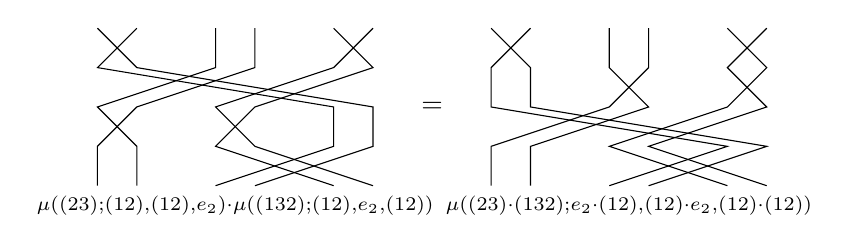
\begin{tikzpicture}[scale=0.5]
    \draw (1,0) -- (2,-1) -- (8,-2) -- (8,-3) -- (5,-4);
    \draw (2,0) -- (1,-1) -- (7,-2) -- (7,-3) -- (4,-4);
    \draw (4,0) -- (4,-1) -- (1,-2) -- (2,-3) -- (2,-4);
    \draw (5,0) -- (5,-1) -- (2,-2) -- (1,-3) -- (1,-4);
    \draw (7,0) -- (8,-1) -- (5,-2) -- (4,-3) -- (7,-4);
    \draw (8,0) -- (7,-1) -- (4,-2) -- (5,-3) -- (8,-4);
    %
    \node at (9.5,-2) {$=$};
    %
    \draw (11,0) -- (12,-1) -- (12,-2) -- (18,-3) -- (15,-4);
    \draw (12,0) -- (11,-1) -- (11,-2) -- (17,-3) -- (14,-4);
    \draw (14,0) -- (14,-1) -- (15,-2) -- (12,-3) -- (12,-4);
    \draw (15,0) -- (15,-1) -- (14,-2) -- (11,-3) -- (11,-4);
    \draw (17,0) -- (18,-1) -- (17,-2) -- (14,-3) -- (17,-4);
    \draw (18,0) -- (17,-1) -- (18,-2) -- (15,-3) -- (18,-4);
    %
    \node at (4.5,-4.5) {$\scriptstyle \mu\left((23);(12),(12), e_2\right) \cdot \mu\left((132); (12), e_2, (12)\right)$};
    \node at (14.5,-4.5) {$\scriptstyle \mu\left((23)\cdot (132); e_2 \cdot (12), (12) \cdot e_2, (12) \cdot (12)\right)$};
  \end{tikzpicture}
  \end{center}
\end{itemize}
\end{rem}

Action operads are themselves the objects of a category, $\mb{AOp}$. The morphisms of this category are defined below.
\begin{Defi}[(Map of action operads)]\label{Defi:mapaop}
A \textit{map of action operads} $f \colon  \Lambda \rightarrow \Lambda'$ consists of a map $f \colon \Lambda \rightarrow \Lambda'$ of the underlying operads such that
  \begin{enumerate}
    \item $\pi^{\Lambda'} \circ f = \pi^{\Lambda}$ (i.e., $f$ is a map of operads over $\Sigma$) and
    \item each $f_{n} \colon \Lambda(n) \rightarrow \Lambda'(n)$ is a group homomorphism.
  \end{enumerate}
\end{Defi}

\begin{prop}\label{prop:cat-of-aop}
There is a category with 
\begin{itemize}
\item objects the action operads $O$ in $\mb{Sets}$, 
\item morphisms as defined in \cref{Defi:mapaop},
\item identities $1_\Lambda \colon \Lambda \to \Lambda$ given by the identity morphism of $\Lambda$ as an operad,
and
\item composition given by composition of maps of operads.
\end{itemize}
\end{prop}

\begin{nota}[(The category of action operads)]\label{nota:cat_aop}
The category in \cref{prop:cat-of-aop} is called the \emph{category of action operads (in $\mb{Sets}$)}, and is denoted $\mb{AOp}$.
\end{nota}

\begin{prop}\label{prop:pi-in-aop}
Let $(\Lambda, \pi)$ be an action operad. The map $\pi \colon \Lambda \rightarrow \Sigma$ is a map of action operads.
\end{prop}


We now study some of the structure on the groups $\Lambda(n)$ for small values of $n$. Recall from \cref{nota:e_identity} that we write $e_{n}$ for the identity element in the group $\Lambda(n)$.
Many of our proofs rely on the following version of the Eckmann-Hilton argument.

\begin{prop}[(Eckmann-Hilton argument)]\label{prop:EH}
Let $G$ be a group with identity element $e$, and suppose $\varphi \colon G \times G \to G$ is a function. If $\varphi$ is a homomorphism, meaning that
\[
\varphi(g',h') \cdot \varphi(g,h) = \varphi(g' \cdot g, h' \cdot h),
\]
and $\varphi(g,e) = g = \varphi(e,g)$ for all elements $g \in G$, then 
\[
\varphi(g, h) = g \cdot h
\]
and $G$ is abelian.
\end{prop}

\begin{lem}\label{lem:calclem}
Let $\Lambda$ be an action operad.
\begin{enumerate}
\item In $\Lambda(1)$, the identity element for the group structure, $e_1$, is equal to the identity element for the operad structure, $\id$.
\item The equation
  \[
    \mu(e_{n}; e_{i_{1}}, \ldots, e_{i_{n}}) = e_{I}
  \]
holds for any natural numbers $n, i_{j}, I = \sum_{j=1}^n i_{j}$.
\item The group $\Lambda(1)$ is abelian.
\end{enumerate}
\end{lem}
\begin{proof}
For the first claim, we will prove that $\id \cdot e_1 = \id \cdot \id$, so $e_1 = \id$ by cancellation.
Note that since the only element of $\Sigma_1$ is the identity permutation, the action operad axiom \cref{eqn:ao_axiom} is
\[
\mu(g';f')\cdot \mu(g;f) = \mu(g'g; f'f)
\]
when $g, g' \in \Lambda(1)$.
Thus we obtain 
\begin{align*}
\id \cdot e_1 & = \mu(\id; \id) \cdot \mu(\id; e_{1}) \\
& = \mu(\id \cdot \id; \id \cdot e_{1}) \\
    &= \mu(\id \cdot \id; \id) \\
    &= \id \cdot \id
\end{align*}
using that $\id$ is the identity element for operadic multiplication, the $n=1$ action operad axiom explained above, that $e_1$ is the identity for group multiplication, and that $\id$ is the identity for operadic multiplication again.
Therefore $\id \cdot e_1 = \id \cdot \id$ as desired, and $e_1 = \id$.

%For the first claim, let $g \in \Lambda(1)$. Then
%  \begin{align*}
%    g & = g \cdot e_{1} \\
%    &= \mu(g; \id) \cdot \mu(\id; e_{1}) \\
%    &= \mu(g \cdot \id; \id \cdot e_{1}) \\
%    &= \mu(g \cdot \id; \id) \\
%    &= g \cdot \id
%  \end{align*}
%using that $e_{1}$ is the unit element for the group structure, that $\id$ is a two-sided unit for operad multiplication, and the final axiom for an action operad together with the fact that the only element of the symmetric group $\Sigma_{1}$ is the identity permutation. Thus $g = g \cdot \id$, so $\id = e_{1}$.

For the second claim, we write $\mu(e_{n}; e_{i_{1}}, \ldots, e_{i_{n}})$ as $\mu(e; \underline{e})$, and consider the square of this element. We find that
  \begin{align*}
    \mu(e; \underline{e}) \cdot \mu(e; \underline{e}) & = \mu(e \cdot e; \underline{e} \cdot \underline{e}) \\
    &= \mu(e; \underline{e}),
  \end{align*}
where the first equality follows from the last action operad axiom together with the fact that $e$ gets mapped to the identity permutation; here $\underline{e} \cdot \underline{e}$ is the sequence $e_{i_{1}} \cdot e_{i_{1}}, \ldots, e_{i_{n}} \cdot e_{i_{n}}$. Thus $\mu(e; \underline{e})$ is an idempotent element of the group $\Lambda(I)$, so must be the identity element $e_{I}$.

For the final claim, note that the specific operadic multiplication map $\mu \colon \Lambda(1) \times \Lambda(1) \rightarrow \Lambda(1)$ is a group homomorphism following from the action operad axioms, and $\id = e_{1}$ is a two-sided unit, so \cref{prop:EH} shows that $\mu$ is actually group multiplication and that $\Lambda(1)$ is abelian.
\end{proof}

\begin{lem}\label{lem:G0abel}
Let $\Lambda$ be an action operad. For any $g, h \in \Lambda(0)$, the equation
\[
g \cdot h = \mu(e_2; g,h)
\]
holds. As a consequence, $\Lambda(0)$ is abelian.
\end{lem}
\begin{proof}
The function $\Lambda(0) \times \Lambda(0) \to \Lambda(0)$ given by
\[
g, h \mapsto \mu(e_2; g, h)
\]
is a group homomorphism by the action operad axiom \cref{eqn:ao_axiom} as we verify below.
\[
\mu(e_2; g', h') \cdot \mu(e_2; g, h) = \mu(e_2 \cdot e_2; g' \cdot g, h' \cdot h) = \mu(e_2; g' \cdot g, h' \cdot h)
\]
In order to apply \cref{prop:EH} and conclude that $g \cdot h = \mu(e_2; g, h)$, we must verify that 
\[
\mu(e_2; e_0, g) = g = \mu(e_2; g, e_0)
\]
for all $g \in \Lambda(0)$.
We will prove the first equality and leave the second to the reader, as it follows in a similar fashion.

By the identity axiom for an operad and the first part of \cref{lem:calclem}, we have $g = \mu(\id; g) = \mu(e_1; g)$ for any $g \in \Lambda(0)$.
By the second part of \cref{lem:calclem}, we also have the equality $e_1 = \mu(e_2; e_0, e_1)$.
Then
  \begin{align*}
   g & = \mu(e_1; g) \\
    &= \mu(\mu(e_2; e_0, e_1); g) \\
    & = \mu(\mu(e_2; e_0, e_1); \mu(e_1; g)) \\
    & = \mu(e_2; e_0, g),
  \end{align*}
  where the final equality follows from operadic associativity together with $g = \mu(e_1; g)$.
  This calculation shows $g = \mu(e_2; e_0, g)$ as desired, and thus proves that the function $\mu(e_2; -,-)$ satisfies the hypotheses in \cref{prop:EH}.
  Therefore $g \cdot h = \mu(e_2; g,h)$ and $\Lambda(0)$ is abelian.
%  Note first that
%    \begin{align*}
%      \mu(e_2; g, h) &= \mu(e_2 \cdot e_2; g \cdot e_0, e_0 \cdot h) \\
%      &= \mu(e_2; g, e_0) \cdot \mu(e_2; e_0, h),
%    \end{align*}
%  so for the first claim that $\mu(e_2; g, h) = g \cdot h$ it will suffice to show that $\mu(e_2; g, e_0) = g$ and $\mu(e_2; e_0, h) = h$ for all $g, h \in \Lambda(0)$. We will use the fact that $\mu(e_0; ) = e_0$, which follows below from a similar argument found in the second part of \cref{calclem}.
%    \begin{align*}
%      \mu(e_0;)\mu(e_0;) &= \mu\left(e_0^2;\right) \\
%      &= \mu(e_0;).
%    \end{align*}
%  Since $\mu(e_0;)$ is an idempotent element of $\Lambda(0)$, then it must be the identity $e_0$. Now we have this, the following sequence of calculations shows that $\mu(e_2; g, e_0) = g$, while a similar calculation would show that $\mu(e_2; e_0, h) = h$. Using \cref{calclem},
%    \begin{align*}
%      g &= \mu(e_1; g) \\
%      &= \mu(\mu(e_2; e_0, e_1); g) \\
%      &= \mu(e_2; \mu(e_0;), \mu(e_1; g)) \\
%      &= \mu(e_2; e_0, g).
%    \end{align*}
%  It remains to show that $\Lambda(0)$ is abelian, which relies on the coincidence of the operad multiplication and the group operation in $\Lambda(0)$, in an Eckmann-Hilton style argument.
%    \begin{align*}
%      g \cdot h &= \mu(e_2; g, h) \\
%      &= \mu(e_2 \cdot e_2; e_0 \cdot g, h \cdot e_0) \\
%      &= \mu(e_2; e_0, h) \cdot \mu(e_2; g, e_0) \\
%      &= h \cdot g.
%    \end{align*}
\end{proof}

The symmetric operad structure on the symmetric groups in \cref{ex:Sigma} was constructed using the functions $\beta, \delta$ from \cref{Defi:beta-s} and \cref{Defi:delta-s}, respectively.
We are now ready to show that any action operad can be described in this way, as promised in the introductory remarks to this section.

%Note that the operad of symmetric groups $\Sigma$ has its action operad structure determined by two auxiliary operations, which we have previously used to describe particular types of operadic composition as described in \cref{conv1} \eqref{conv:beta_delta} and \cref{exSigma}. Rather than simply being convenient notation for common occurences of operadic composition, we will use these ideas to give a characterisation of action operads. First we recall these notions in more detail in the case of the symmetric operad $\Sigma$. The first operation is the block sum of permutations which we denote by
%  \[
%    \beta \colon \Sigma_{k_{1}} \times \cdots \times \Sigma_{k_{n}} \rightarrow \Sigma_{K},
%  \]
%where $K = \sum k_{i}$. The second is a kind of diagonal map which is defined for any natural number $n$ together with natural numbers $k_{1}, \ldots, k_{n}$. Then
%  \[
%    \delta = \delta_{n; k_{1}, \ldots, k_{n}} \colon \Sigma_{n} \rightarrow \Sigma_{K},
%  \]
%is defined on $\sigma \in \Sigma_{n}$ by permuting the elements $1, 2, \ldots, k_{1}$ together in a block according to the action of $\sigma \in \Sigma_{n}$ on $1$, then $k_{1}+1, \ldots, k_{1}+k_{2}$ together in a block according to the action of $\sigma$ on $2$, and so on. The first of these, $\beta$, is a group homomorphism, while $\delta$ is a sort of twisted homomorphism, and taken together they define operadic multiplication in $\Sigma$.

% \begin{Defi}\label{Defi:aop_bl}
% Let $\Lambda$ be an action operad. For $h_i \in \Lambda(k_i)$ and $g \in \Lambda(n)$, define
%   \begin{align*}
%     \beta(h_{1}, \ldots, h_{n}) &= \mu(e_n; h_{1}, \ldots, h_{n}), \\
%     \delta_{n; k_{1}, \ldots, k_{n}}(g) &= \mu(g; e_{k_1}, \ldots, e_{k_n}).
%   \end{align*}
% \end{Defi}


\begin{thm}\label{thm:charAOp}
An action operad $\Lambda$ determines, and is uniquely determined by, the following: 
\begin{itemize}
\item groups $\Lambda(n)$ together with group homomorphisms $\pi_{n} \colon \Lambda(n) \rightarrow \Sigma_{n}$,
\item a group homomorphism
  \[
    \Lambda(k_{1}) \times \cdots \times \Lambda(k_{n}) \stackrel{\beta}{\longrightarrow} \Lambda(k_{1} + \cdots + k_{n}),
  \]
for each $n > 0$ and $k_{1}, \ldots, k_{n}$\ngnote{Used to have: together with the degenerate case of $n=0$ which then is a group homomorphism $1 \rightarrow \Lambda(0)$. Do we need this?}, and
\item a function of sets
  \[
    \Lambda(n) \stackrel{\delta_{n; k_{1}, \ldots, k_{n}}}{\longrightarrow} \Lambda(k_{1} + \cdots + k_{n})
  \]
for each $n, k_{1}, \ldots, k_{n}$,
\end{itemize}
subject to the axioms below. In what we write below, we use the following notational conventions.
\begin{itemize}
\item The symbols $f,g,h$, with or without subscripts, always refer to an element of some group $\Lambda(n)$.
\item The symbols $j,k,m,n,p$ are all natural numbers, and $i$ is a natural number between 1 and $n$.
\end{itemize}
Axioms:
\begin{enumerate}
\item\label{eq1} The homomorphisms $\beta$ are natural with respect to the maps $\pi_{n}$, where $K = k_{1} + \cdots + k_{n}$.
  \[
    \xy
      (0,0)*+{\Lambda(k_{1}) \times \cdots \times \Lambda(k_{n}) } ="00";
      (0,-15)*+{\Sigma_{k_{1}} \times \cdots \times \Sigma_{k_{n}}  } ="01";
      (40,0)*+{\Lambda(K) } ="20";
      (40,-15)*+{\Sigma_{K} } ="21";
      {\ar^{\beta} "00" ; "20"};
      {\ar^{\pi} "20" ; "21"};
      {\ar_{\pi_1 \times \cdots \times \pi_n} "00" ; "01"};
      {\ar_{\beta} "01" ; "21"};
    \endxy
  \]

\item\label{eq2} The homomorphism $\beta \colon \Lambda(k) \rightarrow \Lambda(k)$ is the identity.
\item\label{eq3} The homomorphisms $\beta$ are associative in the sense that the equation
% \[
% \beta(h_{11}, \ldots, h_{1j_{1}}, h_{21}, \ldots, h_{2j_{2}}, \ldots, h_{nj_{n}}) = \beta\left( \beta(h_{11}, \ldots, h_{1j_{1}}), \ldots, \beta(h_{n1}, \ldots, h_{nj_{n}}) \right)
% \]
\[
  \beta(\underline{h_1},\ldots,\underline{h_n}) = \beta(\beta(\underline{h_1}),\ldots,\beta(\underline{h_n}))
\]
holds, where $\underline{h_i} = h_{i1},\ldots,h_{ij_i}$.
\item\label{eq4} The functions $\delta_{n; k_{1}, \ldots, k_{n}}$ are natural with respect to the maps $\pi_{n}$, where $K = k_1 + \cdots + k_n$.
  \[
    \xy
      (0,0)*+{\Lambda(n)} ="00";
      (40,0)*+{\Lambda(k_{1} + \cdots + k_{n}) } ="20";
      (0,-15)*+{\Sigma_{n}  } ="01";
      (40,-15)*+{\Sigma_{k_{1} + \cdots + k_{n}} } ="21";
      {\ar^{\delta} "00" ; "20"};
      {\ar^{\pi} "20" ; "21"};
      {\ar_{\pi} "00" ; "01"};
      {\ar_{\delta} "01" ; "21"};
    \endxy
  \]


\item\label{eq5} The function $\delta_{n; 1, \ldots, 1} \colon \Lambda(n) \rightarrow \Lambda(n)$ is the identity. The function $\delta_{1;n} \colon \Lambda(1) \to \Lambda(n)$ maps $e_1$ to $e_n$\ngnote{I think something more general is true: any $\delta$ maps $e_n$ to $e_K$}.

\item\label{eq6} The equation $\delta_{n; k_1, \ldots, k_n}(g) \delta_{n; j_1, \ldots, j_n}(h) = \delta_{n; j_1,\ldots,j_n}(gh)$ holds when

  \[
    k_{i} = j_{h^{-1}(i)}.
  \]
\item\label{eq7} The functions $\delta$ are associative in the sense that the equation
% \[
% \delta_{m_1 + \cdots + m_n; p_{11}, \ldots, p_{1m_{1}}, p_{21}, \ldots, p_{nm_{n}}}\left( \delta_{n; m_{1}, \ldots, m_{n}}(f) \right) = \delta_{n; P_{1}, \ldots, P_{n}}(f)
% \]
  \[
    \delta_{m_1 + \cdots + m_n; \underline{p_1},\ldots,\underline{p_n}}\left( \delta_{n; m_{1}, \ldots, m_{n}}(g) \right) = \delta_{n; P_{1}, \ldots, P_{n}}(g)
  \]
holds, where $P_{i} = p_{i1} + \cdots + p_{im_{i}}$ and $\underline{p_i} = p_{i1}, \ldots, p_{im_i}$.
\item\label{eq8} The equation
  \[
    \delta_{n;k_1,\ldots,k_n}(g) \beta(h_{1}, \ldots, h_{n}) = \beta(h_{g^{-1}(1)}, \ldots,  h_{g^{-1}(n)}) \delta_{n;k_{g^{-1}(1)},\ldots,k_{g^{-1}(n)}}(g)
  \]
holds, where $h_{i} \in \Lambda(k_{i})$.
\item\label{eq9} The equation
  \[
    \beta(\delta_{1}(g_{1}), \ldots, \delta_{n}(g_{n})) = \delta_{c}(\beta(g_{1}, \ldots, g_{n}))
  \]
holds, where $\delta_{i}(g_{i})$ is shorthand for $\delta_{k_{i}; m_{i1}, \ldots, m_{ik_{i}}}(g_{i})$ and $\delta_{c}$ is shorthand for
  \[
    \delta_{k_{1}+\cdots + k_{n}; m_{11}, m_{12}, \ldots, m_{1k_{1}}, m_{21}, \ldots, m_{nk_{n}}}.
  \]
\end{enumerate}
\end{thm}

\begin{proof}
Let $\Lambda$ be an action operad, and define 
\begin{align*}\label{eqn:bd-from-aop}
\beta(g_1, \ldots, g_n) & = \mu(e_n; g_1, \ldots, g_n),\\
\delta_{n; k_1, \ldots, k_n}(g) & = \mu(g; e_{k_1}, \ldots, e_{k_n}).
\end{align*}
Since $\pi \colon \Lambda \rightarrow \Sigma$ is an operad map, Axioms \ref{eq1} and \ref{eq4} hold by the definition of the operad structure on $\Sigma$ in \cref{ex:Sigma}. 
Since $\Lambda$ is an operad of sets, Axioms \ref{eq2} and \ref{eq5} follow from the operad unit axioms and the first part of \cref{lem:calclem}, and Axioms \ref{eq3}, \ref{eq7}, and \ref{eq9} follow from the operad associativity axiom and the second part of \cref{lem:calclem}. Axioms \ref{eq6} and \ref{eq8} are special cases of the additional action operad axiom, as is the fact that $\beta$ is a group homomorphism.

Conversely, given the data above, we need only define the operad multiplication, verify the operad unit and multiplication axioms, and finally check the action operad axiom. Multiplication is given by
  \[
    \mu(g; h_{1}, \ldots, h_{n}) = \delta_{n; k_{1}, \ldots, k_{n}}(g) \beta(h_{1}, \ldots, h_{n})
  \]
where $h_{i} \in \Lambda(k_{i})$. The identity element $\id$ for the operad structure is $e_1 \in \Lambda(1)$.

We now verify the operad unit axioms. Let $g, h \in \Lambda(n)$. Then
  \begin{align*}
    \mu(e_1; g) &= \delta(e_1)\beta(g) \\
    &= e_1 \cdot g \\
    &= g, \\
    \mu(h; e_1, \ldots, e_1) &= \delta_{n; 1, \ldots, 1}(h)\beta(e_1, \ldots, e_1) \\
    &= h \cdot e_n \\
    &= h
  \end{align*}
by Axioms \ref{eq2} and \ref{eq5}, together with the fact that $\beta$ is a group homomorphism.
Thus $e_1$ satisfies the identity axioms for operadic multiplication.

For the operad associativity axiom, let
\begin{itemize}
\item $f \in \Lambda(m),$
\item $g_{i} \in \Lambda(n_{i})$ for $i=1, \ldots, m$, and
\item $h_{ij} \in \Lambda(p_{i,j})$ for $i=1, \ldots, m$ and $j=1, \ldots, n_{i}$.
\end{itemize}
Further, let $P_{i} = p_{i1} + \cdots + p_{in_{i}}$ and $\underline{h_i}$ denote the list $h_{i1}, h_{i2}, \ldots, h_{in_{i}}$. We must then show that
  \[
    \mu\big( f; \mu(g_{1}; \underline{h_1}), \ldots, \mu(g_{m}; \underline{h_m}) \big) = \mu\big( \mu(f; g_{1}, \ldots, g_{m}); \underline{h_1}, \ldots, \underline{h_m} \big).
  \]
By definition, the left side of this equation is
  \[
    \delta_{m; P_{1}, \ldots, P_{m}}(f) \beta\big( \mu(g_{1}; \underline{h_1}), \ldots, \mu(g_{m}; \underline{h_m}) \big),
  \]
and
  \[
    \mu\left(g_{i}; \underline{h_i}\right) = \delta_{n_{i}; p_{i1}, \ldots, p_{in_{i}}}(g_{i})\beta\left(h_{i1}, \ldots, h_{in_{i}}\right).
  \]
From this point, we suppress subscripts on the $\delta$'s.
Since $\beta$ is a group homomorphism, we can then rewrite the left side as
  \[
    \delta(f)\beta\big(\delta(g_{1}), \ldots, \delta(g_{m})\big)\beta\big(\beta(\underline{h_1}), \ldots, \beta(\underline{h_m})\big)
  \]
where we have suppressed the subscripts on the $\delta$'s. By Axiom \ref{eq3},
  \[
    \beta\big(\beta(\underline{h_1}), \ldots, \beta(\underline{h_m})\big) = \beta\left(\underline{h_1},\ldots,\underline{h_m}\right).
  \]
Furthermore, Axiom \ref{eq9} above shows that
  \[
    \beta\big(\delta(g_{1}), \ldots, \delta(g_{m})\big) = \delta\big(\beta(g_{1}, \ldots, g_{m})\big).
  \]
Thus we have shown that the left side of the operad associativity axiom is equal to
  \[
    \delta(f)\delta\big(\beta(g_{1}, \ldots, g_{m})\big)\beta\left(\underline{h_1},\ldots,\underline{h_m}\right).
  \]
Now the right side is
  \[
    \mu\big( \mu (f; g_{1}, \ldots, g_{m}); \underline{h_1}, \ldots, \underline{h_m} \big),
  \]
which is by definition
  \[
    \delta\big(\mu (f; g_{1}, \ldots, g_{m})\big)\beta\left(\underline{h_1}, \ldots, \underline{h_m}\right).
  \]
Cancelling the $\beta\left(\underline{h_1}, \ldots, \underline{h_m}\right)$ terms, verifying the operad associativity axiom reduces to showing
\begin{eqn}\label{eqn:opass}
\delta(f)\delta\big(\beta(g_{1}, \ldots, g_{m})\big) = \delta\big(\mu (f; g_{1}, \ldots, g_{m})\big).
\end{eqn}
By the definition of $\mu$,
  \[
    \delta\big(\mu (f; g_{1}, \ldots, g_{m})\big) = \delta\big(\delta(f)\beta(g_{1}, \ldots, g_{m}) \big)
  \]
which is itself equal to
\begin{eqn}\label{eqn:opass2}
\delta\big(\delta(f)\big) \delta\big(\beta(g_{1}, \ldots, g_{m})\big)
\end{eqn}
by Axiom \ref{eq6} above. 
Now the $\delta(f)$ on the left side of \cref{eqn:opass} uses $\delta_{n; P_{1}, \ldots, P_{n}}$, while the $\delta(\delta(f))$ in \cref{eqn:opass2} is actually
  \[
    \delta_{m_1 + \cdots + m_{n}; q_{ij}}(\delta_{n; m_{1}, \ldots, m_{n}} (f))
  \]
where the $q_{ij}$ are defined, by Axiom \ref{eq6}, to be given by
  \[
    q_{ij} = p_{i,g_{i}^{-1}(j)}
  \]
using the compatibility of $\beta$ and $\pi$ in Axiom \ref{eq1}. By Axiom \ref{eq7}, this composite of $\delta$'s  is then $\delta_{n; Q_{1}, \ldots, Q_{n}}$ where $Q_{i} = q_{i1} + \cdots + q_{im_{i}}$. But by the definition of the $q_{ij}$, we immediately see that $Q_{i} = P_{i}$, so the $\delta(f)$ in \cref{eqn:opass} is equal to the $\delta(\delta(f))$ appearing in \cref{eqn:opass2}, concluding the proof of the operad associativity axiom.

Writing $\mu(g;\underline{h}) = \mu\left(g; h_{1}, \ldots, h_{n}\right)= $ and $\mu(g';\underline{h'}) = \mu\left(g'; h_{1}', \ldots, h_{n}'\right)$, the action operad axiom is now the calculation below, and uses Axioms \ref{eq4} and \ref{eq8}.
\begin{small}
  \begin{align*}
    \mu(g;\underline{h})\mu(g';\underline{h'}) &= \delta\left(g\right) \beta\left(h_{1}, \ldots, h_{n}\right) \delta\left(g'\right) \beta\left(h_{1}', \ldots, h_{n}'\right) \\
    &= \delta\left(g\right) \delta\left(g'\right) \beta\left(h_{g'(1)}, \ldots, h_{g'(n)}\right)  \beta\left(h_{1}', \ldots, h_{n}'\right) \\
    &= \delta\left(gg'\right) \beta\left(h_{g'(1)}h_{1}', \ldots, h_{g'(n)}h_{n}'\right) \\
    &= \mu\left(gg'; h_{g'(1)}h_{1}', \ldots, h_{g'(n)}h_{n}'\right)
  \end{align*}
\end{small}
\end{proof}

\begin{prop}[Corollary 2.17,  \cite{zhang-grp}]\label{prop:surjortriv} Let $\Lambda$ be an action operad. Then the homomorphisms $\pi_n \colon \Lambda(n) \rightarrow \Sigma_n$ are either all surjective or all the zero map.
\end{prop}
\begin{proof}
% QQQ New short snazzy proof: It's basically the same, but the \beta and \delta axioms allow it to go through a bit more cleanly and less `handwavy'.
We will prove each case separately. The two cases coincide for $n = 0, 1$ as both $\Sigma_0, \Sigma_1$ are the trivial group and therefore any homomorphism with one of them as its codomain is both surjective and the zero map. Since $\Sigma_2$ only has one non-identity element, any homomorphism $G \rightarrow \Sigma_2$ must necessarily be surjective or the zero map.

Suppose that $\pi_2 \colon \Lambda(2) \rightarrow \Sigma_2$ is surjective, so there exists $g \in \Lambda(2)$ such that $\pi_2(g) = \trans{1}{2}$. Let $n>2$. Since $\Sigma_n$ is generated by the adjacent transpositions $\trans{a}{a+1}$, we will show that each such element is in the image of $\pi_n$. Write $\underline{x}^i$ for the $i$-tuple $x, x, \ldots, x$. Then $\trans{a}{a+1} = \beta(\underline{e_1}^{a-1} ,\trans{1}{2},\underline{e_1}^{n-a-1})$ in $\Sigma$, so
  \begin{align*}
      \trans{a}{a+1} &= \beta(\underline{e_1}^{a-1},\trans{1}{2},\underline{e_1}^{n-a-1}) \\ &= \beta(\underline{\pi_1(e_1)}^{a-1},\pi_2(g),\underline{\pi_1(e_1)}^{n-a-1}) \\
      &= \pi_n(\beta(\underline{e_1}^{a-1},g,\underline{e_1}^{n-a-1}))
  \end{align*}
by Axiom \ref{eq1} of \ref{thm:charAOp}.
Thus $\pi_n$ is surjective for all $n>2$ if $\pi_2$ is surjective.

Now we will consider the case where $\pi_2$ is the zero map.
Suppose that there exists $g \in \Lambda(n)$ such that $\pi_n(g) = \sigma \neq e_n$ in $\Sigma_n$.
Then we can find $1 \leq i < j \leq n$ such that $\sigma(j) < \sigma(i)$.
Consider the element 
\[
h = \delta_{n; \underline{0}^{i-1}, 1, \underline{0}^{j-i-1}, 1, \underline{0}^{n-j}}(g) \in \Lambda(2).
\]
By the assumption that $\pi_2$ is the zero map, we must have that $\pi_2(h) = e_2$, but by Axiom \ref{eq4} of \ref{thm:charAOp} we also compute
\[
\pi_2(h) = \delta_{n; \underline{0}^{i-1}, 1, \underline{0}^{j-i-1}, 1, \underline{0}^{n-j}}\big( \pi_n(g) \big) =  \delta_{n; \underline{0}^{i-1}, 1, \underline{0}^{j-i-1}, 1, \underline{0}^{n-j}}\big( \sigma \big).
\]
The element $\delta_{n; \underline{0}^{i-1}, 1, \underline{0}^{j-i-1}, 1, \underline{0}^{n-j}}\big( \sigma \big)$ is equal to $\trans{1}{2}$ by the choice of $i, j$ and \cref{Defi:delta-s}.
These two computations of $\pi_2(h)$ are in contradiction, so there must be no such $g \in \Lambda(n)$.
Thus if $\pi_2$ is the zero map, so is $\pi_n$ for all $n>2$.
%
%
%Assume that $\pi_n$ is zero for some $n \geq 2$. Now let $\sigma \in \operatorname{Im} \pi_{n+1}$, so there exists $g \in \Lambda(n+1)$ such that $\pi_{n+1}(g) = \sigma$. Now $\delta_{n+1;\underline{1},0,\underline{1}}(\sigma)$ is an element of $\Sigma_n$ and
%  \begin{align*}
%    \delta_{n+1;\underline{1},0,\underline{1}}(\sigma) &= \delta_{n+1;\underline{1},0,\underline{1}}(\pi_{n+1})(g) \\
%    &= \pi_n(\delta_{n+1;\underline{1},0,\underline{1}}(g)) \\
%    &= e_n,
%  \end{align*}
%using Axiom \ref{eq4} of \ref{thm:charAOp}. Hence $\sigma = e_{n+1}$ or $\sigma = \trans{a}{a+1}$.
%
%If $\sigma = e_{n+1}$ then $\pi_{n+1}$ is zero. But if $a \neq 1$, then using Axiom \ref{eq4} again
%  \begin{align*}
%    \trans{a-1}{a} &= \delta_{n+1;0,\underline{1}}(\trans{a}{a+1}) \\
%    &= \delta_{n+1;0,\underline{1}}(\pi_{n+1}(g)) \\
%    &= \pi_n(\delta_{n+1;0,\underline{1}}(g)) \\
%    &= e_n,
%  \end{align*}
%a contradiction. If $a = 1$, then $\trans{a}{a+1} = \trans{1}{2}$ and again using Axiom \ref{eq4}
%  \begin{align*}
%    \trans{1}{2} &= \delta_{n+1;\underline{1},0}(\trans{a}{a+1}) \\
%    &= \delta_{n+1;\underline{1},0}(\pi_{n+1}(g)) \\
%    &= \pi_n(\delta_{n+1;\underline{1}}(g),0) \\
%    &= e_n,
%  \end{align*}
%again a contradiction. Hence $\sigma = e_{n+1}$ and so the image of $\pi_{n+1}$ is trivial.

% QQQ Old long proof:
% We will prove each case separately. The two cases coincide for $n = 0$ and $n = 1$ as $\pi_0$ and $\pi_1$ are both the zero map and since $\Sigma_0$ and $\Sigma_1$ are the trivial group then these maps are also surjective.

% Any homomorphism $G \rightarrow \Sigma_2$ must necessarily be surjective or the zero map. To begin we will show that if $\pi_2 \colon \Lambda(2) \rightarrow \Sigma_2$ is surjective then, by induction, the rest of the maps $\pi_n$ are also surjective. If $\pi_2$ is surjective then there exists an element $g_{1,1} \in \Lambda(2)$ such that $\pi_2(g_{1,1}) = \trans{1}{2}$. Now assume that for some $j \geq 2$ that $\pi_j$ is surjective. In particular, this means that for each transposition $\trans{a}{a+k} \in \Sigma_j$, where $1 \leq a \leq j-1$ and $a + k \leq j$, there exists $g_{a,k} \in \Lambda(j)$ such that $\pi_j(g_{a,k}) = \trans{a}{a+k}$. We will use these assumptions to show that each transposition in $\Sigma_{j+1}$ can be written as the image under $\pi_{j+1}$ of some element in $\Lambda(j+1)$, hence any permutation in $\Sigma_{j+1}$ can similarly be written.


% Let $\trans{a}{a+k} \in \Sigma_j$, where $1 \leq a \leq j$ and $a + k \leq j+1$. If $a + k \leq j$, then $\trans{a}{a+k} = \trans{a}{a+k}(j + 1) \in \Sigma_{j+1}$. This transposition can be written as
%   \begin{align*}
%     \trans{a}{a+k} &= \mu^{\Sigma}(e_2 ; \trans{a}{a+k}, e_1) \\
%               &= \mu^{\Sigma}(\pi_2(e_2); \pi_j(g_{a,k}), \pi_1(e_1)) \\
%               &= \pi_{j+1}\left(\mu^{\Lambda}(e_2; g_{a,k},e_1)\right).
%   \end{align*}
% Similarly, if $a > 1$ then this transposition can be written as
%   \begin{align*}
%    \trans{a}{a+k} &= \mu^{\Sigma}(e_2 ; e_1, \trans{a-1}{a+k-1}) \\
%               &= \mu^{\Sigma}(\pi_2(e_2); \pi_1(e_1), \pi_j(g_{a-1,k})) \\
%               &= \pi_{j+1}\left(\mu^{\Lambda}(e_2; e_1, g_{a-1,k})\right).
%   \end{align*}
% Finally, if $a = j$ and $k = 1$, then $\trans{a}{a+k} = \trans{j}{j+1}$. This can be written as
%   \begin{align*}
%     (j \,\,\, j + 1) &= \mu^{\Sigma}(e_2 ; e_{j-1}, (1 \,\,\, 2)) \\
%               &= \mu^{\Sigma}(\pi_2(e_2); \pi_{j-1}(e_{j-1}), \pi_2(g_{1,1})) \\
%               &= \pi_{j+1}\left(\mu^{\Lambda}(e_2; e_{j-1}, g_{1,1})\right).
%   \end{align*}
% Hence $\pi_{j+1}$ is surjective and so all $\pi_n$ are surjective.

% Now instead suppose that $\pi_2 \colon \Lambda(2) \rightarrow \Sigma_2$ is the zero map. Assume that $\pi_j \colon \Lambda(j) \rightarrow \Sigma_j$ is the zero map for some $j \geq 2$. Letting $\sigma \in \textrm{Im}\,\pi_{j+1}$, there exists $g \in \Lambda(j+1)$ such that $\pi_{j+1}(g) = \sigma$. We can then consider the elements $\mu^\Sigma(\sigma; \underline{e_1}, e_o, \underline{e_1})$ where $\underline{e_1}$ means a sequence of $e_1$'s and with $e_0$ in the $k$th position, with $1 \leq k \leq j + 1$. Now
%   \begin{align*}
%     \mu^\Sigma(\sigma; \underline{e_1}, e_o, \underline{e_1}) &= \mu^\Sigma(\pi_{j+1}(g); \underline{\pi_1(e_1)}, \pi_0(e_0), \underline{\pi_1(e_1)}) \\
%     &= \pi_j(\mu^\Lambda(g; \underline{e_1}, e_0, \underline{e_1})) \\
%     &= e_j.
%   \end{align*}
% We can think of this permutation as being $\sigma$ with the $k$th string removed - in \cref{rem:crossed} we comment on such `face' and `degeneracy' maps as used here, and see \cite{ber-simplicial} for a more careful treatment of this idea. Now each of these is the identity $e_j$, as shown above. This means that $\sigma$ must either have been the identity $e_{j+1}$ or a transposition of the form $\trans{a}{a+1}$, where $1 \leq a \leq j$.

% If $\sigma$ is the identity $e_{j+1}$, then we are done since this would give $\textrm{Im}\,\pi_{j+1} = \{e_{j+1}\}$. Instead suppose that $\sigma = \trans{a}{a+1} \in \Sigma_{j + 1}$. Then if $1 < a \leq j$ we can use this to give
%   \begin{align*}
%     \trans{a-1}{a} &= \mu^\Sigma(\trans{a}{a+1}; e_0, \underline{e_1}) \\
%     &= \mu^\Sigma(\pi_{j+1}(g);\pi_0(e_0), \underline{\pi_1(e_1)}) \\
%     &= \pi_j(\mu^\Lambda(g; e_0, \underline{e_1})) \\
%     &= e_j.
%   \end{align*}
% This gives a contradiction, hence $\sigma \neq \trans{a}{a+1}$ and must be the identity $e_{j+1}$.

% Similarly, if $\sigma = \trans{1}{2} \in \Sigma_{j+1}$, then in $\Sigma_j$ we find that
%   \begin{align*}
%     \trans{1}{2} &= \mu^\Sigma(\trans{1}{2} ; \underline{e_1}, e_0) \\
%     &= \mu^\Sigma(\pi_{j+1}(g); \underline{\pi_1(e_1)}, \pi_0(e_0)) \\
%     &= \pi_j(\mu^\Lambda(g ; \underline{e_1}, e_0)) \\
%     &= e_j.
%   \end{align*}
% Again, a contradiction, hence $\sigma = e_{j+1}$.
\end{proof}



\section{Examples}\label{sec:aop-examples}

In this section, we expand our collection of examples  and non-examples of action operads. 
In all but one case, \cref{ex:abgp-aop}, the examples we provide have appeared elsewhere.
The non-examples we provide were largely sourced from questions received after preliminary talks on this research by the authors. 

\begin{example}[(Action operad of braid groups)]\label{example:aop-braid}
One can form an operad $B$ where $B(n)$ is the underlying set of the $n$th braid group, $B_{n}$.
We define the operad structure using the functions $\beta, \delta$ from \cref{rem:br-op-needed}.
Yau checks that these groups and functions satisfy the axioms of an action operad in \cite[Prop 5.2.5]{yau_infinity_2021}, but we note that each of the nine axioms in \cref{thm:charAOp} follows immediately by using the geometric definitions of $\beta, \delta$.
%
%
%Copied:
%
%In order to make sense of this definition, we must define $\beta(\tau_1,\ldots,\tau_n)$ and $\delta(\sigma)$ in the context of braids. The first is the block sum in the obvious sense:  given $n$ different braids on $k_{1}, \ldots, k_{n}$ strands, respectively, we form a new braid on $k_{1} + \cdots + k_{n}$ strands by taking a disjoint union where the braid $\tau_{i}$ is to the left of $\tau_{j}$ if $i < j$. The braid $\delta(\sigma)$ is obtained by replacing the $i$th strand with $k_{i}$ consecutive strands, all of which are braided together according to $\sigma$. These operations are sometimes referred to as `cabling' operations for braids, as described in, for example, \cite{doucot_local_2025}.
%
%Copied 2:
%
%One can form an operad $B$ where $B(n)$ is the underlying set of the $n$th braid group, $B_{n}$. This is done in much the same way as we did for the symmetric operad using the `cabling' operations for braids described after \cref{broperad}. The collections of maps $\pi_{n} \colon B_{n} \rightarrow \Sigma_{n}$ giving the underlying permutation of each braid constitutes an operad map (of non-symmetric or braided operads) operads $Br \rightarrow \Sigma$.
\end{example}

\begin{Defi} For each $n \in \mathbb{N}$, the \emph{ribbon braid group} $RB_{n}$ is the group whose presentation is the same as that of the braid group $B_{n}$, except with the addition of $n$ new generators $t_1, \ldots, t_n$, known as the \emph{twists}. These twists all commute with one other, and also commute with all braids except in the following cases:
  \begin{align*}
    b_i \cdot t_i &= t_{i+1} \cdot b_i,\\
    b_i \cdot t_{i+1} &= t_i \cdot b_i.
  \end{align*}
The \emph{ribbon braid operad} $RB$ is then the operad made up of these groups in a way that extends the definition of the braid operad. In other words, the identity is still $e_1 \in RB_1$, and the operadic multiplication is built up in stages in exactly the same ways as in \cref{broperad}, but with some additional rules for dealing with twists. With regards to the tensor product, we have that for any twist $t_i \in RB_{n}$,
  \[
    t_i = e_{i-1} \otimes t \otimes e_{n-i}
  \]
where $t$ is the sole twist in $RB_1$, and for the `block twists' $t_{(m)}$ we again work recursively:
  \[
    t_{(0)} = e_n, \quad \quad \quad t_{(m+m')} = \left(t_{(m)} \otimes t_{(m')}\right) \cdot b_{(m', m)} \cdot b_{(m, m')}
  \]
\end{Defi}

Much as the symmetric groups can be represented by crossings of a collection of strings, and the braid groups by braidings of strings, the ribbon braid groups deal with the ways that one can braid together several flat ribbons, including the ability to twist a ribbon about its own axis by 360 degrees. The actual definition of the ribbon braid groups is as the fundamental group of a configuration space in which points have labels in the circle, $S^{1}$; see \cite{sal-wahl}.
\begin{center} \begin{tabular}{ccc}
			
\begin{tikzpicture}[baseline]
				\node(xl1) at (-0.7,1){};
				\node(xr1) at (-0.3,1){};
				\node(yl1) at (0.3,1){};
				\node(yr1) at (0.7,1){};
				\node(yl2) at (-0.7, -1){};
				\node(yr2) at (-0.3, -1){};
				\node(xl2) at (0.3, -1){};
				\node(xr2) at (0.7, -1){};
				\node(b) at (0,0)[circle,fill=white, minimum size=0.5cm]{};
       				\draw[rounded corners](xl1.north) to (-0.7,0.5) to (0.3,-0.5) to (xl2.south);
       				\draw[rounded corners](xr1.north) to (-0.3,0.5) to (0.7,-0.5) to (xr2.south);
				\begin{pgfonlayer}{bg}
				\draw[rounded corners](yl1.north) to (0.3, 0.5) to (-0.7, -0.5) to (yl2.south);
				\draw[rounded corners](yr1.north) to (0.7, 0.5) to (-0.3, -0.5) to (yr2.south);
    				\end{pgfonlayer}
				\draw(xl1.north) to (xr1.north);
				\draw(xl2.south) to (xr2.south);
				\draw(yl1.north) to (yr1.north);
				\draw(yl2.south) to (yr2.south);
			\end{tikzpicture} & \quad \quad \quad \quad \quad \quad \quad &
			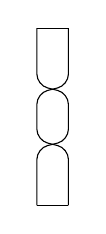
\begin{tikzpicture}[baseline]
				\node(xl1) at (-0.2,1){};
				\node(xr1) at (0.2,1){};	
				\node(xl2) at (-0.2, -1){};
				\node(xr2) at (0.2, -1){};
				\draw[rounded corners](xl1.north) to (-0.2,0.4) to (0.2, 0.3) to (0.2, -0.3) to (-0.2, -0.4) to (xl2.south);	
       				\draw[rounded corners](xr1.north) to (0.2,0.4) to (-0.2, 0.3) to (-0.2, -0.3) to (0.2, -0.4) to (xr2.south);
				\draw(xl1.north) to (xr1.north);
				\draw(xl2.south) to (xr2.south);	
			\end{tikzpicture} \\
			$b$ & & $t$ 
\end{tabular} \end{center}
% This operad $RB$ is also clearly an action operad, since we can just define $\pi^{RB}_n \colon RB_{n} \rightarrow \Sigma_n$ to act like $\pi^B_n$ on any braids, at which point the fact that $\pi(t) \in S_1 = \{e_1\}$ will automatically take care of the twists.

\begin{example}[(Action operad of cactus groups)]\label{ex:cactus-aop}
%\begin{enumerate}
%\item We now describe two less trivial action operads, those given by the braid groups (\cref{ex:braid_operad_B}), $\Lambda = B$, and the ribbon braid groups, $\Lambda = RB$. In each case, the homomorphism $\pi$ is given by taking underlying permutations, and the operad structure is given geometrically by using the procedure explained after \cref{broperad}. For $RB$, the fact that $\pi(t) \in \Sigma_1 = \{e_1\}$ automatically takes care of the twists. We refer the reader to \cite{fie-br} for more information about braided operads, and to \cite{sal-wahl, wahl-thesis} for information about the ribbon case.
The operad of $n$-fruit cactus groups defined by Henriques and Kamnitzer in \cite{hk-cobound} has an action operad structure that we will discuss in \cref{sec:exex-cactus}.
%\end{enumerate}
\end{example}

\begin{example}[(Action operad from an abelian group)]\label{ex:abgp-aop}
Every abelian group $A$ gives rise to an action operad $A^{\bullet}$ as follows. The group $A^{\bullet}(n)$ is the direct sum of $n$ copies of $A$, $A^{n}$. The identity element is required to be $e \in A^{1}$, and the multiplication is defined by
  \[
    \mu((a_{1}, \ldots, a_{n}); \underline{b_1}, \ldots, \underline{b_n}) = (a_{1}+\underline{b_{1}}, a_{2} + \underline{b_{2}}, \ldots, a_{n} + \underline{b_{n}})
  \]
where $\underline{b_{i}}$ is the string $b_{i1}, \ldots, b_{ik_{i}}$, and $a_{i} + \underline{b_{i}}$ is
  \[
    a_{i} + b_{i1}, a_{i} + b_{i2}, \ldots, a_{i} + b_{ik_{i}}.
  \]
The map $\pi_n \colon A^\bullet(n) \rightarrow \Sigma_n$ is the zero map. 
\end{example}

The characterisation of action operads in terms of maps $\pi$, $\beta$, and $\delta$ as in the above \cref{thm:charAOp} allows us to more easily check for counterexamples, as we show in the latter examples below. Some of these, such as the cyclic groups, reflexive groups, and hyperoctahedral groups, do however form crossed simplicial groups as described in \cref{rem:crossed}.

\begin{example}[(Non-examples: subgroups of symmetric groups)]\label{ex:counterex1}
By \cref{prop:surjortriv}, the only action operad $\pi \colon \Lambda \to \Sigma$ for which the homomorphisms $\pi_n$ are injective but not surjective is the action operad of trivial groups. 
Thus there is no family of proper, nontrivial subgroups of the symmetric groups that admits an action operad structure.
In particular, the families of cyclic groups $\{ C_n \}$, reflexive groups $\Lambda(n) = C_2$ of \cite{Kra87}, and alternating groups $\{ A_n \}$ do not admit action operad structures.
\end{example}

\begin{example}[(Non-example: hyperoctahedral groups)]\label{ex:counterex2}
Copied:

n Example 2.28 of \cite{zhang-grp}, Zhang describes one way in which the sequence of hyperoctahedral groups $H_n = C_2 \wr \Sigma_n$ do not form an action operad. We clarify that counterexample here, while also describing another. Elements of $H_n$ can be thought of as signed permutations or, equivalently, as $n \times n$ invertible matrices whose entries consist of $-1$, $0$, or $1$ and in which each row and column has exactly one non-zero entry. E.g., we can consider an element of $H_3$ as a permutation matrix and a $3$-tuple of elements of $C_2 = \{-1,1\}$, or simply as a signed permutation matrix:
  \[
    \left(\trans{2}{3}
    ;
    -1,1,-1\right)
    =
    \left(\begin{bmatrix}
    1 & 0 & 0 \\
    0 & 0 & 1 \\
    0 & 1 & 0
    \end{bmatrix}
    ;
    -1,1,-1\right)
    =
    \begin{bmatrix}
    -1 & 0 & 0 \\
    0 & 0 & -1 \\
    0 & 1 & 0
    \end{bmatrix}
    \in H_3.
  \]

In order to describe the hyperoctahedral groups as an action operad, we could use \cref{thm:charAOp} and define maps $\pi$, $\beta$, and $\delta$. The obvious map $\pi_n \colon H_n \rightarrow \Sigma_n$ takes the `absolute value' of a signed permutation matrix, giving back simply the underlying permutation. It seems obvious then to define $\beta$ to be the block sum of signed permutation matrices, in much the same way as for the symmetric groups. E.g.,
  \[
    \beta\left(
      \begin{bmatrix}
      -1 & 0 & 0 \\
      0 & 0 & -1 \\
      0 & 1 & 0
      \end{bmatrix},
      \begin{bmatrix}
      0 & 1 \\
      -1 & 0
      \end{bmatrix}
    \right)
    =
    \begin{bmatrix}
      -1 &  0 &  0 &  0 & 0 \\
      0  &  0 & -1 &  0 & 0 \\
      0  &  1 &  0 &  0 & 0 \\
      0  &  0 &  0 &  0 & 1 \\
      0  &  0 &  0 & -1 & 0
    \end{bmatrix}.
  \]
For the maps $\delta$, there seems to be two sensible options to try. The first captures Zhang's counterexample by first taking $r_n$ to be the order-reversing signed permutation matrix where all entries are $-1$, i.e., the $n \times n$ matrix with $-1$ in every entry of the anti-diagonal. Then we can define $\delta_{n;k_1,\ldots,k_n}(\sigma)$ to be the block sum $\beta(-r_{k_1},\ldots,-r_{k_n})$ acted on by the product of $r_n$ and $\sigma$. For example,
  \begin{align*}
    \delta_{3;2,1,3}\left(
    \begin{bmatrix}
      -1 & 0 & 0 \\
      0 & 0 & -1 \\
      0 & 1 & 0
      \end{bmatrix}
      \right)
      &=
      \left(
      r_3
      \begin{bmatrix}
      -1 & 0 & 0 \\
      0 & 0 & -1 \\
      0 & 1 & 0
      \end{bmatrix}
      \right)
      \ast
      \begin{bmatrix}
      -r_2 & 0 & 0 \\
      0 & -r_1 & 0 \\
      0 & 0 & -r_3
      \end{bmatrix}\\
&=
    \begin{bmatrix}
      0 & -1 & 0 \\
      0 & 0 & 1 \\
      1 & 0 & 0
      \end{bmatrix}
      \ast
      \begin{bmatrix}
      -r_2 & 0 & 0 \\
      0 & -r_1 & 0 \\
      0 & 0 & -r_3
      \end{bmatrix}\\
      &= \begin{bmatrix}
      0 & r_1 & 0\\
      0 & 0 & -r_3 \\
      -r_2 & 0 & 0
      \end{bmatrix}.
    \end{align*}
In particular, this gives $\delta_{1;n}([-1]) = r_n$ as in \cite{zhang-grp}. Taking $\sigma = (\trans{2}{3};-1,1,-1)$, as above, we can show that Axiom \ref{eq8} fails in \cref{thm:charAOp}. The left-hand side of the axiom would be
        \[
          \delta_{1;3}([-1])\beta(\sigma) = r_n \cdot \sigma =
          \begin{bmatrix}
          0 & -1 & 0 \\
          0 & 0 & 1 \\
          1 & 0 & 0
          \end{bmatrix}
        \]
However, the right-hand side of the axiom would be
  \[
    \beta(\sigma)\delta_{1;3}([-1]) = \sigma \cdot r_n =
    \begin{bmatrix}
    0 & 0 & 1 \\
    1 & 0 & 0 \\
    0 & -1 & 0
    \end{bmatrix}.
  \]
Clearly defining $\delta_{n;k_1,\ldots,k_n}(\sigma) = (\sigma \cdot r_n) \ast \beta(-r_{k_1},\ldots,-r_{k_n})$ would run into the same problem.

An alternative way of defining $\delta$ is to take $\delta_{n;k_1,\ldots,k_n}(\sigma) = \sigma \ast \beta(e_{k_1},\ldots,e_{k_n})$, without involving the order-reversing permutation $r_n$, having the effect of making $\delta_{1;n}([-1]) = -I_n$. This then does satisfy Axiom \ref{eq8}, but fails Axiom \ref{eq6} instead; working through the following counterexample shows this to be the case:
  \begin{align*}
    \delta_{3;2,1,3}\left(
    \begin{bmatrix}
    -1 & 0 & 0 \\
    0 & 0 & 1 \\
    0 & -1 & 0
    \end{bmatrix}
    \right)
    &\delta_{3;3,1,2}\left(
    \begin{bmatrix}
    0 & 0 & 1 \\
    0 & -1 & 0 \\
    -1 & 0 & 0
    \end{bmatrix}
    \right)\\
    &\neq
    \delta_{3;3,1,2}\left(
    \begin{bmatrix}
    -1 & 0 & 0 \\
    0 & 0 & 1 \\
    0 & -1 & 0
    \end{bmatrix}
    \begin{bmatrix}
    0 & 0 & 1 \\
    0 & -1 & 0 \\
    -1 & 0 & 0
    \end{bmatrix}
    \right).
  \end{align*}
\end{example}

%\begin{enumerate}
%\item Cyclic groups: In this case we would want to have $\Lambda(n) = C_n$, the cyclic group of order $n$, with $\pi_n$ being the underlying permutation. But these simply don't form an operad if we are to emulate the composition operation from the symmetric operad $\Sigma$. E.g., by denoting the generator of $C_n$ by $c_n$:
%  \begin{align*}
%    \mu(c_4 ; c_2, c_2) &= (1 \,\, 2 \,\, 3 \,\, 4)\trans{1}{2}\trans{3}{4} \\
%    &= \trans{1}{3} \\
%    &\neq c_4^n
%  \end{align*}
%for any $n \in \{1,2,3,4\}$.
%\item Reflexive groups \cite{Kra87}: Here we would like to take $\Lambda(n) = C_2 = \{e, c_2\}$ with $\pi_n(c_2)$ being the order-reversing permutation on $n$ elements. With these groups and the underlying permutations as described, we find that Axiom \ref{eq1} of \cref{thm:charAOp} is not satisfied. Either $\beta(c_2,c_2) = c_2$ or $\beta(c_2,c_2) = e$. Now
%  \[
%    \beta(\pi_2(c_2),\pi_2(c_2)) = \beta(\trans{1}{2},\trans{1}{2}) = \trans{1}{2}\trans{3}{4}.
%  \]
%But in the case that $\beta(c_2,c_2) = c_2$, then
%  \[
%    \pi_4(\beta(c_2,c_2)) = \pi_4(c_2) = \trans{1}{4}\trans{2}{3} \neq \trans{1}{2}\trans{3}{4}.
%  \]
%In the other case, then
%  \[
%    \pi_4(\beta(c_2,c_2)) = \pi_4(e) = e_4 \neq \trans{1}{2}\trans{3}{4}.
%  \]
%\item
% Hyperoctahedral groups: Can't remember what this fails to satisfy... Dan Graves came up with a counterexample, using the main action operad equivariance axiom, which was clearer than Zhang's description \cite{zhang-grp} - Example 2.28. Can show now that this is really saying that it fails Axiom \ref{eq8} of \cref{thm:charAOp} when taking $\delta_{1;n}(-1)$ to be the order-reversing permutation. If considering elements of the hyperoctahedral groups to be signed permutation matrices, then it may be the case that this works if taking $\delta_{1;n}(-1)$ to be the negative identity matrix.

% In Example 2.28 of \cite{zhang-grp}, Zhang describes how the sequence of hyperoctahedral groups $H_n = C_2 \wr \Sigma_n$ do not form an action operad, despite naturally being a crossed simplicial group. Thanks to Dan Graves, we can also describe directly which axioms of \cref{thm:charAOp} fail to be satisfied, clarifying Zhang's counterexample. On the one hand, if we take $\delta_{1;n}(-1)$ to be the order-reversing permutation, then this fails to satisfy Axiom \ref{eq8} of \cref{thm:charAOp}.

% QQQ Need to revisit this and remember how it works. Certain that it doesn't work for $\delta_{1;k}(\tau) = r_k$, but need to carefully check for when $\delta(\sigma)$ is a `permuted signed block identity' matrix(???).
%\item Alternating groups: If we take $\beta$ and $\delta$ to be analogues of the same maps for the symmetric groups, then we can easily produce non-even permutations using $\delta$: $\delta_{4;,0,0,1,1}(\trans{1}{2}\trans{3}{4})=\trans{1}{2} \notin A_2$ or $\delta_{4;1,1,1,2}(\trans{1}{2}\trans{3}{4}) = \trans{1}{2}\trans{3}{4}\trans{4}{5} \notin A_5$.
%\end{enumerate}
%\end{example}

\begin{rem}\label{rem:crossed}
The crossed simplicial groups of Krasauskas \cite{Kra87} and Fiedoriwicz and Loday \cite{FL91} are related to action operads in the following way. 
On objects, we define a functor $C \colon \mathbf{AOp} \rightarrow \mathbf{CSGrp}$ from the category of action operads to the category of crossed simplicial groups by defining $C(\Lambda)(n) = \Lambda(n+1)$. 
The face and degeneracy maps of the underlying simplicial structure are defined using the operadic composition of $\Lambda$ as in \cite[Construction~1.1]{Kra96} or \cite[Section~2]{ber-simplicial}. 
On morphisms, something\ngnote{is it just $C(f)(n) = f_{n+1}$? That seems conservative to me}.
This functor is neither faithful nor conservative.
\end{rem}
%Salvatore-Wahl:  Framed disks operads\ldots
% \begin{nota}\label{beta_to_oplus}
% Leaning more heavily into the interpretation that the operations denoted $\beta$ above are block sums, we also write $g_1 \oplus g_2 \oplus \cdots \oplus g_n$ for
% $\beta(g_1, g_2, \ldots, g_n)$.
% \end{nota}




\section{Action Operads as Extensions}

In this short section, we situate action operads between operads in the category of groups and symmetric operads.
We prove two main results.
In \cref{prop:Z}, we prove that operads in the category of groups are precisely the same as action operads for which the homomorphisms $\pi_n$ are all the zero map; these are called ``non-crossed group operads'' in \cite{zhang-grp}.
We then turn to studying kernels, images, and short exact sequences of action operads.
We finally prove, in \cref{cor:extension}, that every action operad with surjective $\pi_n$'s can be expressed as an extension of the action operad $\Sigma$ by an operad in the category of groups.

\begin{rem}[(Operads in the category of groups)]\label{rem:op-in-grp}
The category $\mb{Grp}$ of groups and group homomorphisms is symmetric monoidal using the cartesian product of groups.
Thus we can form the category of operads in the category of groups, denoted $\mb{Op}(\mb{Grp})$, as in \cref{rem:V-and-coll}.
The objects of this category are operads $P$ in $\mb{Sets}$ with the additional data of a group structure on each $P(n)$ such that operadic multiplication is a group homomorphism and $\id = e_1$ in $P(1)$; morphisms $f \colon P \to Q$ are those maps of operads such that $f_n \colon P(n) \to Q(n)$ is a group homomorphism for each $n$.
\end{rem}

\begin{prop}\label{prop:Z-obj}
Let $P$ be an operad in $\mb{Grp}$. Then there is an action operad, denoted $Z(P)$, with
\begin{itemize}
\item $Z(P)(n) = P(n)$,
\item the same operadic multiplication as $P$, and
\item each $\pi_n \colon P(n) \to \Sigma_n$ the zero map.
\end{itemize}
Furthermore, if $\Lambda$ is an action operad for which each $\pi_n$ is the zero map, then the groups $\Lambda(n)$ define an operad in $\mb{Grp}$ using the operadic multiplication of $\Lambda$.
\end{prop}
\begin{proof}
It is easy to verify, using \cref{eqn:ao_axiom} of \cref{Defi:aop}, that the operadic multiplication $\mu$ of an action operad is a group homomorphism if and only if $\pi_{n}$ is zero for all $n$.
\end{proof}

\begin{prop}\label{prop:Z}
The assignment on objects $P \mapsto Z(P)$ extends to a functor 
\[
Z \colon  \mb{Op}(\mb{Grp}) \rightarrow \mb{AOp}.
\]
This functor is full, faithful, and its image at the level of objects is precisely the collection of action operads $\Lambda$ for which each $\pi_n$ is the zero map.
\end{prop}
\begin{proof}
Let $f \colon P \to Q$ be a morphism in $\mb{Op}(\mb{Grp})$, meaning that $f$ consists of a family of group homomorphisms $f_n \colon P(n) \to Q(n)$ that define a map of operads.
Define $Z(f)_n = f_n$. We must check that these functions define a map of action operads; functoriality will follow immediately, as composition and identities in both $\mb{Op}(\mb{Grp})$ and $\mb{AOp}$ are given levelwise.
Since each action operad $Z(P)$ has $\pi_n$ the zero map for all $n$, the first numbered axiom in \cref{Defi:mapaop} is satisfied trivially.
The second numbered axiom follows from the definition of a morphism in $\mb{Op}(\mb{Grp})$.
This completes the proof that $Z(f)$ is a map of action operads, and the same reasoning shows that every map of action operads $g \colon Z(P) \to Z(Q)$ is $Z(g')$ for a unique $g' \colon P \to Q$ in $\mb{Op}(\mb{Grp})$, thus $Z$ is full and faithful.
\end{proof}

\begin{prop}\label{prop:im-and-ker-aop}
Let $f \colon \Lambda \to \Lambda'$ be a map of action operads.
\begin{enumerate}
\item The groups
  \[
    \mathrm{Ker}\,f_n = \{x \in \Lambda(n)~\colon~f(x) = e_{n} \}
  \]
form an action operad for which the inclusion $\mathrm{Ker}\,f \hookrightarrow \Lambda$ is a map of action operads.
\item The groups
  \[
    \mathrm{Im}\,f_n = \{f(x)~\colon~x \in \Lambda(n)\}
  \]
form an action operad for which the inclusion $\mathrm{Im}\,\pi \hookrightarrow \Lambda'$ is a map of action operads.
\end{enumerate}
\end{prop}
\begin{proof}
For the first part, we start by defining $\pi_n^{\mathrm{Ker}\,f} \colon \mathrm{Ker}\,f_n \to \Sigma_n$ as the composite group homomorphism
\[
\mathrm{Ker}\,f_n \hookrightarrow \Lambda(n) \stackrel{\pi_n^{\Lambda}}{\to} \Sigma_n.
\]
Since $\pi^{\Lambda} = \pi^{\Lambda'} \circ f$, the composites $\pi_n^{\mathrm{Ker}\,f}$ are all the zero map.
Next we verify that the subgroups $\mathrm{Ker}\,f_n$ are closed under operadic multiplication. 
Let $y \in \mathrm{Ker}\,f_n$ and $x_i \in \mathrm{Ker}\,f_{k_i}$ for $i=1, \ldots, n$.
Then
\begin{align*}
f \big( \mu(y; x_1, \ldots, x_n) \big) & = \mu\big( f(y); f(x_1), \ldots, f(x_n) \big) \\
& = \mu(e_n; e_{k_1}, \ldots, e_{k_n} ) \\ 
& = e_{k_1 + \cdots + k_n}
\end{align*}
by the assumption that $f$ is a map of operads, that $y$ and each $x_i$ is in the kernel, and \cref{lem:calclem}, showing that the kernel subgroups are closed under operadic multiplication.
The operadic identity $\id \in \Lambda(1)$ is an element of $\mathrm{Ker}\,f_1$ because it is equal to $e_1$ by \cref{lem:calclem}.
Thus the groups $\mathrm{Ker}\,f_n$ form a sub-operad of $\Lambda$, and the action operad axiom \cref{eqn:ao_axiom} of \cref{Defi:aop} for $\mathrm{Ker}\,f$ follows immediately from the same axiom for $\Lambda$.
This completes the proof of the first claim, and in fact shows, via \cref{prop:Z-obj}, that these groups constitute an operad in $\mb{Grp}$.

For the second part, we start by defining $\pi_n^{\mathrm{Im}\,f} \colon \mathrm{Im}\,f_n \to \Sigma_n$ as the composite group homomorphism
\[
\mathrm{Im}\,f_n \hookrightarrow \Lambda'(n) \stackrel{\pi_n^{\Lambda'}}{\to} \Sigma_n.
\]
These subgroups are closed under operadic multiplication in $\Lambda'$ using that $f$ is a map of action operads.
The operadic identity $\id \in \Lambda'(1)$ is an element of $\mathrm{Im}\,f_1$ because it is equal to $e_1$ by \cref{lem:calclem}.
This completes the proof that the groups $\mathrm{Im}\,f_n$ form a sub-operad of $\Lambda'$, and the action operad axiom \cref{eqn:ao_axiom} of \cref{Defi:aop} for $\mathrm{Im}\,f$ follows immediately from the same axiom for $\Lambda'$, finishing the proof of the second claim.
\end{proof}

\begin{example}[(Action operads of pure braids, pure ribbon braids)]\label{ex:pure-braids}
%Thus we see that an action operad is either an operad in groups, or is an extension of $\Sigma$ by an operad in groups. 
The $n$th pure braid group, $PB_n$, is defined as the kernel of the homomorphism $\pi_n \colon B_n \to \Sigma_n$, or equivalently as the subgroup of the $n$th braid group consisting of those braids with underlying permutation the identity.
\cref{prop:im-and-ker-aop} gives a simple proof that the pure braid groups form an operad in the category of groups.
Similarly, the pure ribbon braid group, $PRB_n$, is defined as the kernel of $\pi_n \colon RB_n \to \Sigma_n$, and these groups also constitute an operad in the category of groups.

\end{example}

\begin{rem}[(Kernels and images of $\pi$)]\label{rem:im-and-ker-Sigma}
We note that if $(\Lambda, \pi)$ is an action operad, then we can apply the results of \cref{prop:im-and-ker-aop} to $\pi$ by \cref{prop:pi-in-aop}.
The action operad $\mathrm{Ker}\,\pi_n$ will then be an operad in groups, and the action operad $\mathrm{Im}\,\pi_n$ will be a sub-action operad of $\Sigma$.
By \cref{prop:surjortriv}, this means that the action operad $\mathrm{Im}\,\pi_n$ is either $\Sigma$ or the trivial action operad $T$ (\cref{example:aop-triv}).
\end{rem}

%We have the following corollary.
%\begin{cor}\label{corZ}
%For an action operad $\Lambda$, the sets
%  \[
%    \mathrm{Ker}\,\pi_n = \{g \in \Lambda(n)~\colon~\pi_{n}(g) = e_{n} \}
%  \]
%form an action operad for which the inclusion $\mathrm{Ker}\,\pi \hookrightarrow \Lambda$ is a map of action operads.
%\end{cor}
%\begin{proof}
%For $\textrm{Ker}\,\pi \hookrightarrow \Lambda$ to be a map of action operads, we must define the map $\textrm{Ker}\,\pi \rightarrow \Sigma$ to be zero,  and we must check that the operadic multiplication of elements in the kernel is also in the kernel. This last fact is a trivial consequence of $\pi$ being an operad map.
%\end{proof}
%
%\begin{cor}\label{image}
%For an action operad $\Lambda$, the sets
%  \[
%    \mathrm{Im}\,\pi_n = \{\pi_n(g)~\colon~g \in \Lambda(n)\}
%  \]
%form an action operad for which the inclusion $\mathrm{Im}\,\pi \hookrightarrow \Sigma$ is a map of action operads.
%\end{cor}
%\begin{proof}
%The operad multiplication of elements in the image is also in the image, as is the unit element in $\mathrm{Im}\,\pi_1$, following again as a consequence of $\pi$ being an operad map. The map $\mathrm{Im}\,\pi \hookrightarrow \Sigma$ is an inclusion and so is immediately seen to be a map of action operads.
%\end{proof}

\begin{Defi}\label{Defi:ses-aop}
A \emph{short exact sequence of action operads} consists of action operads $\Lambda_1, \Lambda_2, \Lambda_3$ and maps of action operads $f \colon \Lambda_1 \to \Lambda_2$, $g \colon \Lambda_2 \to \Lambda_3$ such that
\begin{itemize}
\item the action operad $\mathrm{Ker}\,f$ is the trivial action operad $T$,
\item the action operad $\mathrm{Im}\,f$ is the action operad $\mathrm{Ker}\,g$, and
\item the action operad $\mathrm{Im}\,g$ is the action operad $\Lambda_3$.
\end{itemize}
We denote such a short exact sequence as
\[
T \to \Lambda_1 \stackrel{f}{\to} \Lambda_2 \stackrel{g}{\to} \Lambda_3 \to T,
\]
and we say that a short exact sequence exhibits \emph{$\Lambda_2$ as an extension of $\Lambda_3$ by $\Lambda_1$}.
\end{Defi}

The following corollary puts \cref{rem:im-and-ker-Sigma} into the language of short exact sequences and extensions.

\begin{cor}\label{cor:extension}
Let $(\Lambda, \pi)$ be an action operad and assume that every homomorphism $\pi_n \colon \Lambda(n) \to \Sigma_n$ is surjective.
Then there is a short exact sequence of action operads
%Every action operad $\Lambda$ with nontrivial $\pi$ fits into a short exact sequence
  \[
    T \rightarrow \mathrm{Ker}\,\pi \hookrightarrow \Lambda \stackrel{\pi}{\longrightarrow} \Sigma \rightarrow T.
  \]
%by which we mean this is a sequence of action operad maps which is an exact sequence of groups at each $n$.
\end{cor}

\section{Presentations for Action Operads}

This section details how to provide presentations for action operads using the theory of locally finitely presentable (lfp) categories.
We refer the reader to \cite{ar} for a full treatment of lfp categories.
Our treatment here diverges slightly from how one might give presentations for symmetric operads because it is necessary to build in the underlying permutation map $\pi \colon \Lambda \to \Sigma$ from the beginning.
In the theory of plain operads, the starting point is a collection: sets $\{ P(n) \}$ indexed by the natural numbers.
In the theory of symmetric operads, these are enhanced to symmetric collections: sets $\{ P(n) \}$ indexed by the natural numbers, together with a right action $P(n) \times \Sigma_n \to P(n)$.
Our analogue of collections (see \cref{Defi:coll-over-SS}) are now sets $P(n)$, indexed by natural numbers, equipped with functions $\pi_n \colon P(n) \to \Sigma_n$.
Thus the natural notion of the arity of an element in an action operad is not a natural number $n$, but rather a pair $(n, \sigma)$ where $\sigma \in \Sigma_n$.

\begin{Defi}[(Collections over $\SS$)]\label{Defi:coll-over-SS}
  Let $\SS$ be the set that is the disjoint union of the underlying sets of all the symmetric groups. Then $\mb{Sets}/\SS$ is the slice category over $\SS$ with objects $(X,f)$ where $X$ is a set and $f \colon X \rightarrow \SS$ and morphisms $(X_{1}, f_{1}) \rightarrow (X_{2}, f_{2})$ are those functions $g \colon X_{1} \rightarrow X_{2}$ such that $f_{1} = f_{2}g$. We call an object $(X,f)$ a \textit{collection over $\SS$}, and say that an element $x \in X$ has \emph{underlying permutation $\sigma$} if $f(x) = \sigma$.
\end{Defi}

\begin{nota}\label{nota:Xofsigma}
If $(X, f)$ is a collection over $\SS$, we write $X(\sigma)$ for $f^{-1}(\sigma)$. In other words, $X(\sigma)$ is the set of elements of $X$ with underlying permutation $\sigma \in \Sigma_n \subseteq \SS$.
\end{nota}

\begin{thm}\label{thm:aop-lfp}
The category $\mb{AOp}$ of action operads is a variety of $\SS$-sorted finitary algebras, and therefore is a finitary monadic category over $\mb{Sets}/\SS$. In particular, $\mb{AOp}$ is locally finitely presentable.
\end{thm}
\begin{proof}
In order to prove that $\mb{AOp}$ is a variety of $\SS$-sorted finitary algebras (henceforth shortened to \emph{$\mb{AOp}$ is a variety}), we must define a set $\mathcal{O}$ of operation symbols and a set of equations $E$ such that action operads are the 
\begin{itemize}
\item collections $(X, f)$ over $\SS$, 
\item equipped with functions
\[
X(\theta) \colon X(\sigma_1) \times \cdots \times X(\sigma_n) \to X(\sigma)
\]
for each operation symbol $\theta \in \mathcal{O}$ of type $\theta \colon \sigma_1, \ldots, \sigma_n \to \sigma$,
\item satisfying the equations in $E$.
\end{itemize}
The set $\mathcal{O}$ of operation symbols is defined to have the elements given below.
\begin{enumerate}
\item For each $\sigma, \tau \in \Sigma_n$, we define an operation symbol
\[
\star[\sigma, \tau] \colon \sigma, \tau \to \sigma \tau,
\]
where the target $\sigma \tau$ is the product of these permutations in $\Sigma_n$.
\item For each natural number $n$, we define an operation symbol
\[
U_n \colon \to e_n,
\]
where the source is the empty list of permutations and the target is the identity element $e_n \in \Sigma_n$.
\item For each $\sigma \in \Sigma_n$, we define an operation symbol
\[
i[\sigma] \colon \sigma \to \sigma^{-1}.
\]
\item Let $\mu$ denote the operadic multiplication in the operad of symmetric groups, $\Sigma$, from \cref{ex:Sigma}. For each $\sigma \in \Sigma_n$ and $\tau_i \in \Sigma_{k_i}$ for $i=1, \ldots, n$, we define an operation symbol $\theta[\sigma; \tau_i]$ of type
\[
\theta[\sigma; \tau_i] \colon \sigma, \tau_1, \ldots, \tau_n \to \mu(\sigma; \tau_1, \ldots, \tau_n).
\]
\end{enumerate}
The set $E$ of equations is defined to have the elements below.
\begin{enumerate}
\item We write $x \star y$ for $\star[\sigma, \tau](x,y)$, where $x$ is a variable of type $\sigma$ and $y$ is a variable of type $\tau$. For each triple $\rho, \sigma, \tau \in \Sigma_n$, there is an equation
\[
(x \star y) \star z = x \star (y \star z).
\]
\item An $\mathcal{O}$-algebra $X$ has, for each $n$, an element $u_n \in X(e_n)$ given by $U_n$. For each $\sigma \in \Sigma_n$, there are equations
\begin{align*}
u_n \star x & = x,\\
x \star u_n & = x.
\end{align*}
\item We write $x^{-1}$ for $i[\sigma](x)$, where $x$ is a variable of type $\sigma$. For each $\sigma \in \Sigma_n$, there are equations
\begin{align*}
x^{-1} \star x & = u_n,\\
x \star x^{-1} & = u_n.
\end{align*}
\item We write $\theta(x; y_1, \ldots, y_n)$ for $\theta[\sigma; \tau_i](x, y_1, \ldots, y_n)$, where $x$ is a variable of type $\sigma \in \Sigma_n$ and for each $i= 1, \ldots, n$ $y_i$ is a variable of type $\tau_i \in \Sigma_{k_i}$. Then for each 
\begin{itemize}
\item $\rho \in \Sigma_n$;
\item $\sigma_i \in \Sigma_{k_i}$, for $i= 1, \ldots, n$; and
\item $\tau_{i,j} \in \Sigma_{h_{i,j}}$, for $i=1, \ldots, n$ and $j=1, \ldots, k_i$;
\end{itemize}
there is an equation
\begin{multline*}
\theta\big( \theta(x; y_1, \ldots, y_n); z_{1,1}, \ldots, z_{1, k_1}, \ldots, z_{n, k_n} \big) = \\ \theta\big( x; \theta(y_1; z_{1,1}, \ldots, z_{1, k_1}), \ldots, \theta(y_n; z_{n, 1}, \ldots, z_{n, k_n}) \big).
\end{multline*}
\item For each $\sigma \in \Sigma_n$, there are equations
\begin{align*}
\theta(u_1; x)& = x, \\
\theta(x; u_1, \ldots, u_1) & = x.
\end{align*}
\item Let $x$ be a variable of type $\sigma \in \Sigma_i$, $y_i$ be a variable of type $\tau_i \in \Sigma_{k_i}$ for $i=1, \ldots, n$, $x'$ be a variable of type $\sigma' \in \Sigma_n$, and $y_i'$ be a variable of type $\tau_i' \in \Sigma_{\sigma^{-1}(i)}$. Then for each such choice of permutations, there is an equation
\[
\theta(x'; y_1', \ldots, y_n') \star \theta(x; y_1, \ldots, y_n) = \theta(x' \star x; y'_{\sigma(1)} \star y_1, \ldots, y'_{\sigma(n)} \star y_n).
\]
\end{enumerate}

The category of $\mathcal{O}$-algebras satisfying the equations in $E$ is isomorphic to $\mb{AOp}$ as follows. Given such an algebra $(X, f)$, define an action operad $(\Lambda^X, \pi)$ by defining 
\[
\Lambda^X(n) = \coprod_{\sigma \in \Sigma_n} X(\sigma)
\]
and defining $\pi_n \colon X(n) \to \Sigma_n$ to be $f$ restricted to $\Lambda^X(n) \subseteq X$. Each $X(n)$ is a group using $\star$ as its multiplication and $u_n$ as its identity element, and $\pi_n$ is a homomorphism since $\pi_n(x \star y) = \sigma \tau$ when $x \in X(\sigma), y \in X(\tau)$ by the definition of the source and target of $\star$. The operadic multiplication is given by the operation symbols $\theta[\sigma; \tau_i]$, and equations 4 and 5 in $E$ are the operadic associativity and unit axioms, using the first part of \cref{lem:calclem}. The additional action operad axiom is equation 6 in $E$. A morphism of $\mathcal{O}$-algebras is easily seen to define a map of action operads, and these assignments are an isomorphism between the category $\mb{AOp}$ and the category of $\mathcal{O}$-algebras satisfying the equations in $E$.
This completes the proof that $\mb{AOp}$ is the variety defined by $\mathcal{O}$ and $E$. It is therefore a finitary monadic category over $\mb{Sets}/\SS$ by \cite[Thm~3.18]{ar} and locally finitely presentable by \cite[Cor~3.7]{ar}.
\end{proof}


%A useful method for constructing new examples of some given algebraic structure is through the use of presentations. A presentation consists of generating data together with relations between generators using the operations of the algebra involved. In categorical terms, the generators and relations are both given as free gadgets on some underlying data, and the presentation itself is a coequalizer. This section will establish the categorical structure necessary to give presentations for action operads, and then explain how such a presentation is reflected in the associated club and $2$-monad. The most direct route to the desired results uses the theory of locally finitely presentable categories. We recall the main definitions briefly, but refer the reader to \cite{ar} for additional details.
%
%\begin{Defi}\label{def:filtered}
%  A \textit{filtered category} is a nonempty category $C$ such that
%    \begin{itemize}
%      \item if $a,b$ are objects of $C$, then there exists another object $c \in C$ and morphisms $a \rightarrow c, b \rightarrow c$; and
%      \item if $f,g \colon a \rightarrow b$ are parallel morphisms in $C$, then there exists a morphism $h \colon b \rightarrow c$ such that $hf = hg$.
%    \end{itemize}
%\end{Defi}
%
%\begin{Defi}
%  A \emph{filtered colimit} is a colimit over a filtered category.
%\end{Defi}
%
%\begin{Defi}
%  Let $C$ be a category with all filtered colimits. An object $x \in C$ is \textit{finitely presentable} if the representable functor $C(x, -) \colon C \rightarrow \mb{Sets}$ preserves filtered colimits.
%\end{Defi}
%
%\begin{Defi}
%  A \textit{locally finitely presentable category} is a category $C$ such that
%  \begin{itemize}
%    \item $C$ is cocomplete and
%    \item there exists a small subcategory $C_{fp} \subseteq C$ of finitely presentable objects such that any object $x \in C$ is the filtered colimit of some diagram in $C_{fp}$.
%  \end{itemize}
%\end{Defi}
%
%The definition of a locally finitely presentable category has many equivalent variants, but we find this one most practicable to work with in this setting.
%
%\begin{thm}
%The category $\mb{AOp}$ is locally finitely presentable.
%\end{thm}
%\begin{proof}
%First note that we can define a category $\mb{Op}^{g}$, whose objects are operads $P$ in which each $P(n)$ also carries a group structure. This is an equational theory using equations with only finitely many elements, so $\mb{Op}^{g}$ is locally finitely presentable \cite[Corollary 3.7]{ar}. A slice category of a locally finitely presentable category is itself locally finite presentable \cite[Proposition 1.57]{ar} and since the symmetric operad is an object of $\mb{Op}^{g}$, the slice category $\mb{Op}^{g}/\Sigma$ is locally finitely presentable.
%
%There is an obvious inclusion functor $\mb{AOp} \hookrightarrow \mb{Op}^{g}/\Sigma$. Now $\mb{AOp}$ is a full subcategory of $\mb{Op}^{g}/\Sigma$ which is closed under products, subobjects. Since any object of $\mb{Op}^{g}/\Sigma$ isomorphic to an action operad is in fact an action operad, the inclusion   $\mb{AOp} \hookrightarrow \mb{Op}^{g}/\Sigma$ is actually the inclusion of a reflective subcategory. One can easily check that $\mb{AOp}$ is in fact closed under all limits and filtered colimits in $\mb{Op}^{g}/\Sigma$, so by the Reflection Theorem (2.48 in \cite{ar}), $\mb{AOp}$ is locally finitely presentable.
%\end{proof}
%
%
%
%\begin{rem}
%In standard presentations of the theory of operads (see, for example, \cite{mss-op}), a nonsymmetric operad will have an underlying collection (or $\mathbb{N}$-indexed collection of sets) while a symmetric operad will have an underlying symmetric collection (or $\mathbb{N}$-indexed collection of sets in which the $n$th set has an action of $\Sigma_{n}$). Our collections over $\SS$ more closely resemble the former as there is no group action present.
%\end{rem}
%
%\begin{example}
%One can easily form new action operads from old ones by taking limits. To take a limit of a diagram in $\mb{AOp}$, one forgets down to the category of operads over $\Sigma$ and takes the limit there. Concretely, products in $\mb{AOp}$ are computed as products in $\mb{Op}/\Sigma$ which themselves are (possibly wide) pullbacks in the category of operads. This pullback will then be computed levelwise, showing that at each dimension there is a group structure with a group homomorphism to the appropriate $\Sigma_{n}$ and that the final action operad axiom holds since it does in each component. The equalizer of a pair of maps will then just be the levelwise equalizer. This shows that the pointwise product of an action operad $P$ with an action operad of the form $Z(Q)$ (as in \cref{Z}) is again an action operad, but the pointwise product of two arbitrary action operads might not be.
%\end{example}
%\begin{thm}\label{underlyingSS}
%There exists a forgetful functor $U \colon \mb{AOp} \rightarrow \mb{Sets}/\SS$ which preserves all limits and filtered colimits.
%\end{thm}
%
%\begin{proof}
%For a given action operad $\Lambda$, we put $U(\Lambda) = \left(\coprod_{\mathbb{N}} \Lambda(n), \coprod_{\mathbb{N}} \pi_n \right)$ and this easily extends to a mapping on morphisms using the universal property of the coproduct. The preservation of filtered colimits follows from the fact that these are computed pointwise, together with the fact that every map between action operads preserves underlying permutations.
%As equalizers are computed levelwise, and the product $\Lambda \times \Lambda'$ has underlying operad the pullback $\Lambda \times_{\Sigma} \Lambda'$; this pullback is itself computed levelwise. Together, these imply that $U$ also preserves all limits.
%\end{proof}
%

For our purposes, the most important consequence of \cref{thm:aop-lfp} is that we can freely generate an action operad from a collection over $\SS$, as stated below.

\begin{cor}\label{cor:free-aop-fun}
The underlying collection functor $U \colon \mb{AOp} \to  \mb{Sets}/\SS$ has a left adjoint $F \colon \mb{Sets}/\SS \rightarrow \mb{AOp}$, the free action operad functor.
\end{cor}
%\begin{proof}
%The category $\mb{Sets}/\SS$ is locally finitely presentable as it is equivalent to the functor category $[\SS, \mb{Sets}]$ (here $\SS$ is treated as a discrete category) and any presheaf category is locally finitely presentable. The functor $U$ preserves limits and filtered colimits between locally finitely presentable categories, so has a left adjoint (see Theorem 1.66 in \cite{ar}).
%\end{proof}

\begin{Defi}[(Presentation for action operads)]\label{Defi:pres-aop}
  A \textit{presentation} for an action operad $\Lambda$ consists of
  \begin{itemize}
    \item a pair of collections over $\SS$ denoted $\mathbf{g}, \mathbf{r}$,
    \item a pair of maps $s_{1}, s_{2} \colon F\mathbf{r} \rightarrow F\mathbf{g}$ between the associated free action operads, and
    \item a map $p \colon F\mathbf{g} \rightarrow \Lambda$ of action operads exhibiting $\Lambda$ as the coequalizer of $s_{1},s_{2}$.
  \end{itemize}
\end{Defi}

\begin{example}[(The presentation for $\Sigma$)]\label{ex:sigma-pres}
Here we explicitly give a presentation for the action operad of symmetric groups.
Recall that the symmetric group $\Sigma_n$ has a presentation, as a \emph{group}, with
\begin{itemize}
\item generators $\sigma_{1;n}, \ldots, \sigma_{n-1;n}$ and
\item relations
\begin{enumerate}
\item $\sigma_{i;n}^2 = e_n$ for all $i$,
\item $\sigma_{i;n} \sigma_{j;n} = \sigma_{j;n} \sigma_{i;n}$ for $i, j$ satisfying $|i-j| \geq 2$, and
\item $\sigma_{i;n} \sigma_{i+1;n} \sigma_{i;n} = \sigma_{i+1;n} \sigma_{i;n} \sigma_{i+1;n}$ for $1 \leq i < n-1$.
\end{enumerate}
\end{itemize}
\ngmpar{Not super happy with this part, but got the main idea down for now}Note the nonstandard naming of the generators as $\sigma_{i;n}$ instead of merely $\sigma_i$. We have included this additional information in our generators as it is necessary to distinguish between the generators traditionally denoted $\sigma_i$ that are in different symmetric groups. 

Utilizing the operad structure, we notice that
\[
\sigma_{i;n} = \beta(e_{i-1}, \sigma_{1;2}, e_{n-i-1}).
\]
Furthermore, the second relation above is a consequence of this expression, the fact that $\beta$ is a group homomorphism, and the second part of \cref{lem:calclem}.
Thus as an action operad, $\Sigma$ is generated by the single element $\sigma_{1;2} \in \Sigma_2$.
In order to simplify notation, we just write $\sigma$ instead of $\sigma_{1;2}$.

We now define the relations for this presentation of $\Sigma$ as an action operad.
The first relation is 
\begin{equation}\label{eq:rel1}
\sigma^2 = e_2.
\end{equation}
The second relation is
\begin{equation}\label{eq:rel2}
\mu(\sigma; e_1, e_2) = \mu(e_2; e_1, \sigma) \cdot \mu(e_2; \sigma, e_1).
\end{equation}
We therefore claim that $\Sigma$ has a presentation given by
\begin{itemize}
\item $\mathbf{g} = \{ \sigma \}$, defined as a collection over $\SS$ by the function sending $\sigma$ to $(1 \ 2) \in \Sigma_2$;
\item $\mathbf{r} = \{ \rho_1, \rho_2 \}$, defined as a collection over $\SS$ by the function sending $\rho_1$ to $e_2 \in \Sigma_2$ and $\rho_2$ to $(1 \ 3 \ 2) \in \Sigma_3$;
\item $s_1 \colon F\mathbf{r} \to F\mathbf{g}$ defined uniquely by requiring
\begin{align*}
s_1(\rho_1) & = \sigma^2,\\
s_1(\rho_2) & = \mu(\sigma; e_1, e_2);
\end{align*}
\item and $s_2 \colon F\mathbf{r} \to F\mathbf{g}$ defined uniquely by requiring
\begin{align*}
s_2(\rho_1) & = e_2,\\
s_2(\rho_2) & = \mu(e_2; e_1, \sigma) \cdot \mu(e_2; \sigma, e_1).
\end{align*}
\end{itemize}
We note that both $s_1, s_2$ map $\rho_1$ to $(1 \ 2)(1 \ 2) = e_2 \in \Sigma_2$, and both $s_1, s_2$ map $\rho_2$ to $(1 \ 3 \ 2) = (2 \ 3)(1 \ 2)$, thus defining maps of collections over $\SS$.

In order to prove that the above is a presentation for $\Sigma$, we must define a map of action operads $t \colon F\mathbf{g} \to \Sigma$ that exhibits $\Sigma$ as the coequalizer of $s_1, s_2$.
Define $t$ by requiring $t(\sigma) = (1 \ 2)$.
The calculations above prove that $t \circ s_1 = t \circ s_2$, and now we must prove that $t$ is the universal map of action operads coequalizing $s_1, s_2$.
Let $\Lambda$ be an action operad, and $f \colon F\mathbf{g} \to \Lambda$ a map of action operads such that $f \circ s_1 = f \circ s_2$.
We construct a unique map of action operads $\tilde{f} \colon \Sigma \to \Lambda$ such that $f = \tilde{f} \circ t$.
If such an $\tilde{f}$ exists, it must map the transposition $\sigma_{1;2} = (1 \ 2) \in \Sigma_2$ to $f(\sigma)$.
Since each other generator (of $\Sigma_n$ as a group) $\sigma_{i;n}$ is the image
\begin{equation}\label{eq:sig-in}
\sigma_{i;n} = \beta(e_{i-1}, \sigma_{1;2}, e_{n-i-1}) = \mu(e_3; e_{i-1}, \sigma_{1;2}, e_{n-i-1})
\end{equation}
of $\sigma_{1;2}$ under an operadic multiplication, any map of action operads $\tilde{f}$ satisfying $f = \tilde{f} \circ t$ is unique if it exists, and $\tilde{f}_n$ is 
defined on the generators of $\Sigma_n$ using \cref{eq:sig-in} by
\begin{align*}
\tilde{f}_n(\sigma_{i;n}) & = \tilde{f} \big( \mu(e_3; e_{i-1}, \sigma_{1;2}, e_{n-i-1}) \big) \\
& = \mu\big( \tilde{f}_n(e_3); \tilde{f}_n(e_{i-1}), \tilde{f}_n(\sigma_{1;2}), \tilde{f}_n(e_{n-i-1}) \big) \\
& =  \mu(e_3; e_{i-1}, f(\sigma), e_{n-i-1}).
\end{align*}
In order to show that these formulas define a unique homomorphism $\tilde{f}_n \colon \Sigma_n \to \Lambda(n)$, we must check that they respect the relations in the presentation of $\Sigma_n$ given above.
We only check the third axiom, and only in the case $i=1, n=3$; the rest we leave as a simple exercise for the reader.
In order to verify that $\tilde{f}_3$ respects this relation, we must show that
\begin{equation}\label{eq:3term}
\tilde{f}_3( \sigma_{1;3}) \ \tilde{f}_3(\sigma_{2;3} ) \ \tilde{f}_3(\sigma_{1;3} ) = \tilde{f}_3(\sigma_{2;3} ) \ \tilde{f}_3(\sigma_{1;3} ) \ \tilde{f}_3( \sigma_{2;3}).
\end{equation}
By\ngnote{need updated version on my board}, the left side of the above is 
\begin{align*}
\mu\big( e_2; f(\sigma), e_1 \big) \mu\big( e_2; e_1, f(\sigma) \big) \mu\big( e_2; f(\sigma), e_1 \big) & = f \big( \mu(e_2; \sigma, e_1)\mu(e_2;e_1,  \sigma)\mu(e_2; \sigma, e_1) \big).
\end{align*}
Since $f$ is a map of action operads and coequalizes $s_1, s_2$, we obtain
\begin{align*}
f \big( \mu(e_2; \sigma, e_1)\mu(e_2;e_1,  \sigma)\mu(e_2; \sigma, e_1) \big) & = f\big( \mu(e_2; \sigma, e_1) \mu(\sigma; e_1, e_2) \big)
\end{align*}
by the equality $fs_1(\rho_2) = fs_2(\rho_2)$.
Finally, the action operad axiom shows that
\[
f\big( \mu(e_2; \sigma, e_1) \mu(\sigma; e_1, e_2) \big) = f\big( \mu(\sigma; e_1, \sigma) \big).
\]
A similar argument shows that the right side of \cref{eq:3term} is equal to 
\[
f \big(\mu(e_2;e_1, \sigma) \mu(e_2; \sigma, e_1)\mu(e_2;e_1,  \sigma) \big),
\]
and once by coequalizing $s_1, s_2$ is therefore $f\big( \mu(\sigma; e_1, \sigma) \big)$.
We have now verified that $\tilde{f}_n$ respects the relations for the presentation of $\Sigma_n$, and therefore defines a unique group homomorphism $\tilde{f}_n \colon \Sigma_n \to \Lambda(n)$.



\ngnoteil{only thing left is to show $\tilde{f}$'s are an operad map over $\Sigma$}
\end{example}

\section{Action Operads as Clubs}

Kelly's theory of clubs \cite{kelly_club1, kelly_club0, kelly_club2} was designed to simplify and explain certain aspects of coherence results, namely the fact that many coherence results rely on extrapolating information about general free objects for a $2$-monad $T$ from information about the specific free object $T1$ where $1$ denotes the terminal category. This occurs, for example, in the study of the many different flavors of monoidal category:  plain monoidal category, braided monoidal category, symmetric monoidal category, and so on. This section will explain how every action operad gives rise to a club, as well as compute the clubs which arise as the image of this procedure.

We begin by reminding the reader of the notion of a club, or more specifically what Kelly \cite{kelly_club1,kelly_club2} calls a club over $\mb{P}$. We will only be interested in clubs over $\mb{P}$, and thusly shorten the terminology to club from this point onward. Defining clubs is accomplished most succinctly using Leinster's terminology of generalized operads \cite{leinster}.

\begin{Defi}
Let $C$ be a category with finite limits.
\begin{enumerate}
\item A monad $T \colon C \rightarrow C$ is \textit{cartesian} if the functor $T$ preserves pullbacks, and the naturality squares for the unit $\eta$ and the multiplication $\mu$ for $T$ are all pullbacks.
\item The category of \textit{$T$-collections}, $T\mbox{-}\mb{Coll}$, is the slice category $C/T1$, where $1$ denotes the terminal object.
\item Given a pair of $T$-collections $X \stackrel{x}{\rightarrow} T1, Y \stackrel{y}{\rightarrow} T1$, their \textit{composition product} $X \circ Y$ is given by the pullback below together with the morphism along the top.
  \[
    \xy
      (0,0)*+{X \circ Y} ="00";
      (15,0)*+{TY} ="10";
      (30,0)*+{T^{2}1} ="20";
      (45,0)*+{T1} ="30";
      (0,-10)*+{X} ="01";
      (15,-10)*+{T1} ="11";
      {\ar^{} "00" ; "10"};
      {\ar^{Ty} "10" ; "20"};
      {\ar^{\mu} "20" ; "30"};
      {\ar^{T!} "10" ; "11"};
      {\ar_{x} "01" ; "11"};
      {\ar^{} "00" ; "01"};
      (3,-3)*{\lrcorner};
    \endxy
  \]
\item The composition product, along with the unit of the adjunction $\eta \colon 1 \rightarrow T1$, give $T\mbox{-}\mb{Coll}$ a monoidal structure. A \textit{$T$-operad} is a monoid in $T\mbox{-}\mb{Coll}$.
\end{enumerate}
\end{Defi}

\begin{rem}
Everything in the above definition can be $\mb{Cat}$-enriched without any substantial modifications. Thus we require our ground $2$-category to have finite limits in the enriched sense, and the slice and pullbacks are the $2$-categorical (and not bicategorical) versions. If we take this $2$-category to be $\mb{Cat}$, then in each case the underlying category of the $2$-categorical construction is given by the corresponding $1$-categorical version. From this point, we will not distinguish between the $1$-dimensional and $2$-dimensional theory. Our interest, of course, is in the $2$-dimensional version.
\end{rem}

Let $\Sigma$ be the operad of symmetric groups. This is the terminal object of the category of action operads, with each $\pi_{n}$ the identity map. Then $\underline{E\Sigma}$ is a $2$-monad on $\mb{Cat}$, and by results in \cref{sec:propofopsincat} it is cartesian.

\begin{Defi}
A \textit{club} is a $T$-operad in $\mb{Cat}$ for $T = \underline{E\Sigma}$.
\end{Defi}

\begin{rem}
The category $\mb{P}$ in Kelly's terminology is the result of applying $\underline{E\Sigma}$ to $1$, and can be identified with $B\Sigma = \coprod B\Sigma_{n}$.
\end{rem}

It is useful to break down the definition of a club. A club consists of
\begin{enumerate}
\item a category $K$ together with a functor $K \rightarrow B \Sigma$,
\item a multiplication map $K \circ K \rightarrow K$, and
\item a unit map $1 \rightarrow K$
\end{enumerate}
satisfying the axioms to be a monoid in the monoidal category of $E\Sigma$-collections. By the definition of $K \circ K$ as a pullback, objects are tuples of objects of $K$ $(x; y_{1}, \ldots, y_{n})$ where $\pi(x) = n$. A morphism
  \[
    (x; y_{1}, \ldots, y_{n}) \rightarrow (z; w_{1}, \ldots, w_{m})
  \]
exists only when $n=m$ (since $B\Sigma$ only has endomorphisms) and then consists of a morphism $f \colon x \rightarrow z$ in $K$ together with morphisms $g_{i} \colon y_{i} \rightarrow z_{\pi(x)(i)}$ in $K$.

\begin{nota}\label{nota:clubmult}
For a club $K$ and a morphism $(f; g_{1}, \ldots, g_{n})$ in $K \circ K$, we write $f(g_{1}, \ldots, g_{n})$ for the image of the morphism under the functor $K \circ K \rightarrow K$.
\end{nota}

We will usually just refer to a club by its underlying category $K$.


\begin{thm}
Let $\Lambda$ be an action operad. Then the map of operads $\pi \colon \Lambda \rightarrow \Sigma$ gives the category $B\Lambda = \coprod B\Lambda(n)$ the structure of a club.
\end{thm}
\begin{proof}
To give the functor $B\pi \colon B\Lambda \rightarrow B \Sigma$ the structure of a club it suffices (see \cite{leinster}) to show that
\begin{itemize}
\item the induced monad, which we will show to be $\underline{E\Lambda}$, is a cartesian monad on $\mb{Cat}$,
\item the transformation $\tilde{\pi} \colon \underline{E\Lambda} \Rightarrow \underline{E\Sigma}$ induced by the functor $E\pi$ is cartesian, and
\item $\tilde{\pi}$ commutes with the monad structures.
\end{itemize}
The monad $\underline{E\Lambda}$ is always cartesian by results of \cref{sec:propofopsincat}. The transformation $\tilde{\pi}$ is the coproduct of the maps $\tilde{\pi}_{n}$ which are induced by the universal property of the coequalizer as shown below.
  \[
    \xy
      (0,0)*+{\scriptstyle E\Lambda(n) \times \Lambda(n) \times X^n} ="00";
      (0,-15)*+{\scriptstyle E\Sigma_{n} \times \Sigma_{n} \times X^n} ="01";
      (30,0)*+{\scriptstyle E\Lambda(n) \times X^n} ="10";
      (30,-15)*+{\scriptstyle E\Sigma_{n} \times X^n} ="11";
      (60,0)*+{\scriptstyle E\Lambda(n) \times_{\Lambda(n)} X^n} ="20";
      (60,-15)*+{\scriptstyle E\Sigma_{n} \times_{\Sigma_{n}}  X^n} ="21";
      {\ar (11,1)*{}; (22,1)*{} };
      {\ar (11,-1)*{}; (22,-1)*{} };
      {\ar_{E\pi \times \pi \times 1} "00" ; "01"};
      {\ar (10,-14)*{}; (23,-14)*{} };
      {\ar (10,-16)*{}; (23,-16)*{} };
      {\ar_{E\pi \times 1} "10" ; "11"};
      {\ar@{.>}^{\tilde{\pi}_{n}} "20" ; "21"};
      {\ar "10" ; "20"};
      {\ar "11" ; "21"};
    \endxy
  \]
Naturality is immediate, and since $\pi$ is a map of operads $\tilde{\pi}$ also commutes with the monad structures.

It only remains to show that $\tilde{\pi}$ is cartesian and that the induced monad is actually $\underline{E\Lambda}$. Since the monads $\underline{E\Lambda}$ and $\underline{E\Sigma}$ both decompose into a disjoint union of functors, we only have to show that, for any $n$, the square below is a pullback.
  \[
    \xy
      (0,0)*+{\coeq{E\Lambda}{X}{\Lambda}{n}} ="00";
      (0,-10)*+{B\Lambda(n)} ="01";
      (35,0)*+{E\Sigma_{n} \times_{\Sigma_{n}} X^n} ="10";
      (35,-10)*+{B\Sigma_{n}} ="11";
      {\ar^{} "00" ; "10"};
      {\ar^{} "10" ; "11"};
      {\ar^{} "00" ; "01"};
      {\ar^{} "01" ; "11"};
    \endxy
  \]
By \cref{coeq-lem}
%(QQQ happy with this reference? QQQ Seems like the right thing?)
, this amounts to showing that the square below is a pullback.
  \[
    \xy
      (0,0)*+{\left(E\Lambda(n) \times X^n\right)/\Lambda(n)} ="00";
      (0,-10)*+{B\Lambda(n)} ="01";
      (35,0)*+{\left(E\Sigma_{n} \times X^n\right)/\Sigma_{n}} ="10";
      (35,-10)*+{B\Sigma_{n}} ="11";
      {\ar^{} "00" ; "10"};
      {\ar^{} "10" ; "11"};
      {\ar^{} "00" ; "01"};
      {\ar^{} "01" ; "11"};
    \endxy
  \]
Here, $(A \times B)/G$ is the category whose objects are equivalence classes of pairs $(a,b)$ where $(a,b) \sim (ag, g^{-1}b)$, and similarly for morphisms. Now the bottom map is clearly bijective on objects since these categories only have one object. An object in the top right is an equivalence class
  \[
    [\sigma; x_{1}, \ldots, x_{n}] = \left[e; x_{\sigma^{-1}(1)}, \ldots, x_{\sigma^{-1}(n)}\right].
  \]
A similar description holds for objects in the top left, with $g \in \Lambda(n)$ replacing $\sigma$ and $\pi(g)^{-1}$ replacing $\sigma^{-1}$ in the subscripts. The map along the top sends $[g; x_{1}, \ldots, x_{n}]$ to $[\pi(g); x_{1}, \ldots, x_{n}]$, and thus sends $[e; x_{1}, \ldots, x_{n}]$ to $[e; x_{1}, \ldots, x_{n}]$, giving a bijection on objects.

Now a morphism in $(E\Lambda(n) \times X^{n})/\Lambda(n)$ can be given as
  \[
    [e; x_{1}, \ldots, x_{n}] \stackrel{[!; f_{i}]}{\longrightarrow} [g; y_{1}, \ldots, y_{n}].
  \]
Mapping down to $B\Lambda(n)$ gives $ge^{-1} = g$, while mapping over to $(E\Sigma_{n} \times X^{n})/\Sigma_{n}$ gives $[!; f_{i}]$ where $! \colon e \rightarrow \pi(g)$ is now a morphism in $E\Sigma_{n}$. In other words, a morphism in the upper left corner of our putative pullback square is determined completely by its images along the top and lefthand functors. Furthermore, given $g \in \Lambda(n)$, $\tau = \pi(g)$, and morphisms $f_{i} \colon x_{i} \rightarrow y_{i}$ in $X$, the morphism $[! \colon e \rightarrow g; f_{i}]$ maps to the pair $(g, [! \colon e \rightarrow \tau; f_{i}])$, completing the proof that this square is indeed a pullback.
\end{proof}

The club, which we now denote $K_{\Lambda}$, associated to $E\Lambda$ has the following properties. First, the functor $K_{\Lambda} \rightarrow B\Sigma$ is a functor between groupoids. Second, the functor $K_{\Lambda} \rightarrow B\Sigma$ is  bijective-on-objects. We claim that these properties characterize those clubs which arise from action operads. Thus the clubs arising from action operads are very similar to PROPs \cite{mac_prop, markl_prop}.

\begin{thm}\label{thm:club=operad}
Let $K$ be a club such that
\begin{itemize}
\item the map $K \rightarrow B\Sigma$ is bijective on objects and
\item $K$ is a groupoid.
\end{itemize}
Then $K \cong K_{\Lambda}$ for some action operad $\Lambda$. The assignment $\Lambda \mapsto K_{\Lambda}$ is a full and faithful embedding of the category of action operads $\mb{AOp}$ into the category of clubs.
\end{thm}
\begin{proof}
Let $K$ be such a club. Our hypotheses immediately imply that $K$ is a groupoid with objects in bijection with the natural numbers; we will now assume the functor $K \rightarrow B\Sigma$ is the identity on objects. Let $\Lambda(n) = K(n,n)$. Now $K$ comes equipped with a functor to $B\Sigma$, in other words group homomorphisms $\pi_{n} \colon \Lambda(n) \rightarrow \Sigma_{n}$. We claim that the club structure on $K$ makes the collection of groups $\{ \Lambda(n) \}$ an action operad. In order to do so, we will employ \cref{thm:charAOp}.

First, we give the group homomorphism $\beta$ using \cref{nota:clubmult}. Define
  \[
    \beta(g_{1}, \ldots, g_{n}) = e_{n}(g_{1}, \ldots, g_{n})
  \]
 (see \ref{nota:clubmult}) where $e_{n}$ is the identity morphism $n \rightarrow n$ in $K(n,n)$. Functoriality of the club multiplication map immediately implies that this is a group homomorphism. Second, we define the function $\delta$ in a similar fashion:
  \[
    \delta_{n; k_{1}, \ldots, k_{n}}(f) = f(e_{1}, \ldots, e_{n}),
  \]
where here $e_{i}$ is the identity morphism of $k_{i}$ in $K$.

There are now nine axioms to verify in \cref{thm:charAOp}. The club multiplication functor is a map of collections, so a map over $B\Sigma$; this fact immediately implies that Axioms \eqref{eq1} (using morphisms in $K \circ K$ with only $g_{i}$ parts) and \eqref{eq4} (using morphisms in $K \circ K$ with only $f$ parts) hold. The mere fact that multiplication is a functor also implies Axioms \eqref{eq6} (once again using morphisms with only $f$ parts) and \eqref{eq8} (by considering the composite of a morphism with only an $f$ with a morphism with only $g_{i}$'s). Axiom \eqref{eq2} is the equation $e_{1}(g) = g$ which is a direct consequence of the unit axiom for the club $K$; the same is true of Axiom \eqref{eq5}. Axioms \eqref{eq3}, \eqref{eq7},  and \eqref{eq9} all follow from the associativity of the club multiplication.

Finally, we would like to show that this gives a full and faithful embedding
    \[
        K_{-} \colon \mb{AOp} \rightarrow \mb{Club}
    \]
of the category of action operads into the category of clubs. Let $f, f' \colon \Lambda \rightarrow \Lambda'$ be maps between action operads. Then if $K_{f} = K_{f'}$ as maps between clubs, then they must be equal as functors $K_{\Lambda} \rightarrow K_{\Lambda'}$. But these functors are nothing more than the coproducts of the functors
  \[
    B(f_{n}), B(f_{n}') \colon B\Lambda(n) \rightarrow B\Lambda'(n),
  \]
and the functor $B$ from groups to categories is faithful, so $K_{-}$ is also faithful. Now let $f \colon K_{\Lambda} \rightarrow K_{\Lambda'}$ be a maps of clubs. We clearly get group homomorphisms $f_{n} \colon \Lambda(n) \rightarrow \Lambda'(n)$ such that $\pi^{\Lambda}_{n} = \pi^{\Lambda'}_{n} f_{n}$, so we must only show that the $f_{n}$ also constitute an operad map. Using the description of the club structure above in terms of the maps $\beta, \delta$, we are able to see that commuting with the club multiplication implies commuting with both of these, which in turn is equivalent to commuting with operad multiplication. Thus $K_{-}$ is full as well.
\end{proof}

\begin{rem}
First, one should note that being a club over $B\Sigma$ means that every $K$-algebra has an underlying strict monoidal structure. Second, requiring that $K \rightarrow B\Sigma$ be bijective on objects ensures that $K$ does not have  operations other than $\otimes$, such as duals or internal hom-objects, from which to build new types of objects. Finally, $K$ being a groupoid ensures that all of the ``constraint morphisms'' that exist in algebras for $K$ are invertible.

These hypotheses could be relaxed somewhat. Instead of having a club over $B\Sigma$, we could have a club over the free symmetric monoidal category on one object (note that the free symmetric monoidal category monad on $\mb{Cat}$ is still cartesian). This would produce $K$-algebras with underlying monoidal structures which are not necessarily strict. This change should have relatively little impact on how the theory is developed. Changing $K$ to be a category instead of a groupoid would likely have a larger impact, as the resulting action operads would have monoids instead of groups at each level. We have made repeated use of inverses throughout the proofs in the basic theory of action operads, and these would have to be revisited if groups were replaced by monoids in the definition of action operads.
\end{rem}

In \cite{kelly_club1}, Kelly discusses clubs given by generators and relations. His generators include functorial operations more general than what we are interested in here, and the natural transformations are not required to be invertible. In our case, the only generating operations we require are those of a unit and tensor product, as the algebras for $E\Lambda$ are always strict monoidal categories with additional structure. Tracing through his discussion of generators and relations for a club gives the following theorem.

\begin{thm}\label{pres1}
Let $\Lambda$ be an action operad with presentation given by $(\mathbf{g},\mathbf{r}, s_{i}, p)$. Then the club $E\Lambda$ is generated by
\begin{itemize}
  \item functors giving the unit object and tensor product, and
  \item natural transformations given by the collection $\mathbf{g}$:  each element $x$ of $\mathbf{g}$ with $\pi(x) = \sigma_{x} \in \Sigma_{|x|}$ gives a natural transformation from the $n$th tensor power functor to itself,
\end{itemize}
subject to relations such that the following axioms hold.
\begin{itemize}
  \item The monoidal structure given by the unit and tensor product is strict.
  \item The transformations given by the elements of $\mathbf{g}$ are all natural isomorphisms.
  \item For each element $y \in \mathbf{r}$, the equation $s_{1}(y) = s_{2}(y)$ holds.
\end{itemize}
\end{thm}

Bringing this down to a concrete level we have the following corollary.

\begin{cor}\label{pres2}
Assume we have a notion $\mathcal{M}$ of strict monoidal category which is given by  a set natural isomorphisms
  \[
    \mathcal{G} = \left\{ (f, \pi_{f}) \, | \,  x_{1} \otimes \cdots \otimes x_{n} \stackrel{f}{\longrightarrow} x_{\pi_{f}^{-1}(1)} \otimes \cdots \otimes x_{\pi_{f}^{-1}(n)} \right\}
  \]
subject to a set $\mathcal{R}$ of axioms. Each such axiom is given by the data
\begin{itemize}
  \item two finite sets $f_{1}, \ldots, f_{n}$ and $f_{1}', \ldots, f_{m}'$ of elements of $\mathcal{G}$; and
  \item two formal composites $F,F'$ using only composition and tensor product operations and the $f_{i}$, respectively $f_{i}'$, 
\end{itemize}
such that the underlying permutation of $F$ equals the underlying permutation of $F'$ (we compute the underlying permutations using the functions $\beta, \delta$ of \cref{thm:charAOp}). The element $\left(\underline{f}, \underline{f}', F, F'\right)$ of the set $\mathcal{R}$ of axioms corresponds to the requirement that the composite of the morphisms $f_{i}$ using $F$ equals the composite of the morphisms $f_{j}'$ using $F'$ in any strict monoidal category of type $\mathcal{M}$. Then strict monoidal categories of type $\mathcal{M}$ are given as the algebras for the club $E\Lambda$ where $\Lambda$ is the action operad with
\begin{itemize}
  \item $\mathbf{g} = \mathcal{G}$,
  \item $\mathbf{r} = \mathcal{R}$,
  \item $s_{1}$ given by mapping the generator $\left(\underline{f}, \underline{f}', F, F'\right)$ to the operadic composition of the $f_{i}$ using $F$ via $\beta, \delta$, and
  \item $s_{2}$ given by mapping the generator $\left(\underline{f}, \underline{f}', F, F'\right)$ to the operadic composition of the $f_{i}'$ using $F'$ via $\beta, \delta$.
\end{itemize}
\end{cor}

\begin{example}
The $2$-monad for symmetric strict monoidal categories (or permutative categories, as they are known in the topological literature) is given by $E\Sigma$, so the notion of symmetric strict monoidal categories corresponds to the symmetric operad. While this example is well-known, we go into further detail to set the stage for less common examples.

The $2$-monad $\underline{E\Sigma}$ on $\mb{Cat}$ is given by
  \[
    \underline{E\Sigma} (X) = \coprod E\Sigma_{n} \times_{\Sigma_{n}} X^{n}.
  \]
An object of $E\Sigma_{n} \times_{\Sigma_{n}} X^{n}$ is an equivalence class of the form $[\sigma; x_{1}, \ldots, x_{n}]$ where $\sigma \in \Sigma_{n}$ and $x_{i} \in X$. The equivalence relation gives
  \[
    [\sigma; x_{1}, \ldots, x_{n}] = \left[e; x_{\sigma^{-1}(1)}, \ldots, x_{\sigma^{-1}(n)}\right],
  \]
so objects can be identified with finite strings of objects of $X$. Morphisms are given by equivalence classes of the form
  \[
    [\sigma; x_{1}, \ldots, x_{n}] \stackrel{[!; f_{1}, \ldots, f_{n}]}{\longrightarrow} [\tau; y_{1}, \ldots, y_{n}].
  \]
Here $! \colon \sigma \cong \tau$ is the unique isomorphism in $E \Sigma_{n}$, and $f_{i} \colon x_{i} \rightarrow y_{i}$ in $X$. Using the equivalence relation, we find that morphisms between finite strings
  \[
    x_{1}, \ldots, x_{n} \rightarrow y_{1}, \ldots, y_{n}
  \]
are given by a permutation $\rho \in \Sigma_{n}$ together with maps $f_{i} \colon x_{i} \rightarrow y_{\rho(i)}$ in $X$ (note that there are no morphisms between strings of different length); this is a special case of the calculation in \cref{hom-set-lemma}. Thus $E \Sigma(X)$ is easily seen to be the free permutative category generated by $X$, and therefore $\Sigma$-monoidal categories are permutative categories.
\end{example}

\begin{example}
The template above can be used to show that the braid operad $B$ corresponds to the $2$-monad for braided strict monoidal categories. The details are almost exactly the same, only we use braids instead of permutations. The equivalence relation on objects gives
  \[
    [\gamma; x_{1}, \ldots, x_{n}] = \left[e; x_{\pi(\gamma)^{-1}(1)}, \ldots, x_{\pi(\gamma)^{-1}(n)}\right],
  \]
where $\gamma \in B_{n}$ and $\pi(\gamma)$ is its underlying permutation; thus objects of $EB(X)$ are once again finite strings of objects of $X$. A morphism
  \[
    x_{1}, \ldots, x_{n} \rightarrow y_{1}, \ldots, y_{n}
  \]
is then given by a braid $\gamma \in B_{n}$ together with maps $f_{i} \colon x_{i} \rightarrow y_{\pi(\gamma)(i)}$ in $X$. Thus one should view a morphism as given by
\begin{itemize}
\item a finite ordered set $x_{1}, \ldots, x_{n}$ of objects of $X$ as the source,
\item another such finite ordered set (of the same cardinality) $y_{1}, \ldots, y_{n}$ of objects of $X$ as the target,
\item a geometric braid $\gamma \in B_{n}$ on $n$ strands, and
\item for each strand, a morphism in $X$ from the object labeling the source of that strand to the object labeling the target.
\end{itemize}
This is precisely Joyal and Street's \cite{js} construction of the free braided strict monoidal category generated by a category $X$, and thus $B$-monoidal categories are braided strict monoidal categories.

This example can be extended to include ribbon braided categories as well. A \textit{ribbon braid} is given, geometrically, in much the same way as a braid except that instead of paths $[0,1] \rightarrow \mathbb{R}^{3}$ making up each individual strand, we use ribbons
$[0,1] \times [-\varepsilon, \varepsilon] \rightarrow \mathbb{R}^{3}$. This introduces the possibility of performing a full twist on a ribbon, and one can describe ribbon braided categories using generators and relations by introducing a natural twist isomorphism $\tau_{A} \colon A \rightarrow A$ and imposing one relation between the twist and the braid $\gamma_{A,B} \colon A \otimes B \rightarrow B \otimes A$. In \cite{sal-wahl}, the authors show that the ribbon braid groups give an action operad $RB$, and that (strict) ribbon braided categories are precisely the algebras for $ERB$.
\end{example}


\artpart{Operads with Equivariance}\label{part:op-with-eq}

Moved this comment, needs intro and something like below: ``most of this stuff admits an enriched variant''
\begin{rem}
It is possible to consider $\Lambda$-operads in categories other than the category of sets. In this case we still use the notion of an action operad given above, but then take the operad $P$ to have objects $P(n)$ which are the objects of some closed symmetric monoidal category $\mathcal{V}$. We will rarely use anything that might require the closed structure as such, only the fact that the tensor product distributes over colimits in each variable. This is a consequence of the fact that both $X \otimes -$ and $- \otimes X$ are left adjoints in the case of a closed symmetric monoidal category. Thus while we set up the foundations using only operads in $\mb{Sets}$, the diligent reader could easily modify this theory for their closed symmetric monoidal category of choice. In fact, we will use the same theory in $\mb{Cat}$ with its cartesian structure, noting only that the same arguments work in $\mb{Cat}$ with essentially no modification.
\end{rem}
\begin{rem}
The above result can be interpreted for $\Lambda$-operads in an arbitrary cocomplete symmetric monoidal category $\mathcal{V}$ in which the tensor product distributes over colimits in each variable. In order to do so, the following changes must be made. First, cartesian products of objects $X(k)$ must be replaced by the tensor product in $\mathcal{V}$ of the same objects. Second, any product with a hom-set from $B\Lambda$ must be replaced by a copower with the same set (recall that the copower of a set $S$ with an object $X$ is given by the formula $S \odot X = \coprod_{S} X$). The same changes also allow one to interpret the results in the following chapter about algebras in such a category, unless noted otherwise.
\end{rem}


\section{\texorpdfstring{$\Lambda$}{L}-Operads and their Algebras}

This section presents the definition of a $\Lambda$-operad (\cref{Defi:lamop}), where $\Lambda$ is an action operad.
This definition unifies the various types (non-symmetric, symmetric, and braided) of operads discussed in \cref{sec:back-op} under one umbrella term.
The different group actions arise from different choices of $\Lambda$.
We also define algebras over a $\Lambda$-operad in \cref{Defi:aop-alg}, and prove a change-of-action operad result in \cref{prop:pbaop}.

%Just as we had the definitions of operad, symmetric operad, and braided operad, we now come to the general definition of a $\Lambda$-operad,  Thereafter we begin to delve into the theory around $\Lambda$-operads. Beginning by recasting familiar operads as $\Lambda$-operads for particular choices of $\Lambda$, we then proceed to shadow standard operadic definitions for algebras and pseudoalgebras in this setting, characterising algebras using endomorphism $\Lambda$-operads, and deriving monads from $\Lambda$-operads. We show that there is an adjunction between $\Lambda\mbox{-}\mb{Op}$ and $\Sigma\mbox{-}\mb{Op}$, and prove some technical results regarding maps between monads induced by $\Lambda$-operads.
 	% QQQ chapter: operads and algebras with general group actions
 	% \begin{itemize}
 	% 	\item defines $\Lambda$-operads
 	% 	\item goes over familiar examples
 	% 	\item recasts familar operad algebra stuff for $\Lambda$-operads
 	% 	\begin{itemize}
	%  		\item defines algebras and pseudoalgebras for $\Lambda$-operads
	%  		\item characterises algebras using the endomorphism operads
	%  		\item monads via operads
	%  	\end{itemize}
	%  	\item theorem about the adjunction between $\Lambda-\bf{Op}$ and $\bf{\Sigma}-\bf{Op}$
	%  	\item technical results about monad maps
 	% \end{itemize}


\begin{Defi}[($\Lambda$-operads)]\label{Defi:lamop}
  Let $\Lambda$ be an action operad. A \textit{$\Lambda$-operad} $P$ (in $\mb{Sets}$) consists of
    \begin{itemize}
      \item a non-symmetric operad $P$ in $\mb{Sets}$ and
      \item for each $n$, an action $P(n) \times \Lambda(n) \rightarrow P(n)$ of $\Lambda(n)$ on $P(n)$
    \end{itemize}
such that the following two equivariance axioms hold.
  \begin{itemize}
    \item For each $p \in P(n)$, $q_i \in P(k_i)$, and $g_i \in \Lambda(k_i)$ for $i=1, \ldots, n$:
  \[
    \mu^{P}(p; q_{1} \cdot g_{1}, \ldots, q_{n} \cdot g_{n}) = \mu^{P}(p; q_{1}, \ldots, y_{n}) \cdot \beta^{\Lambda}(g_{1}, \ldots, g_{n}).
  \]
    \item For each $p \in P(n)$, $g \in \Lambda(n)$, and $q_i \in \Lambda(k_i)$ for $i=1, \ldots, n$:
  \[
    \mu^{P}(p \cdot g; q_{1}, \ldots, q_{n}) = \mu^{P}\left(p; q_{g^{-1}(1)}, \ldots, q_{g^{-1}(n)}\right) \cdot \delta_{n;k_1,\ldots,k_n}^{\Lambda}(g).
  \]
  \end{itemize}
\end{Defi}


\begin{Defi}[(Map of $\Lambda$-operads)]\label{Defi:aop_map}
Let $P$ and $Q$ be $\Lambda$-operads. A \emph{map $f \colon P \rightarrow Q$ of $\Lambda$-operads} consists of an operad map (\ref{Defi:aop_map}) that is levelwise equivariant with respect to the $\Lambda(n)$-actions, i.e., for each $n \in \mathbb{N}$ the following diagram commutes.
  \[
    \xy
      (0,0)*+{P(n) \times \Lambda(n)}="00";
      (30,0)*+{Q(n) \times \Lambda(n)}="10";
      (30,-15)*+{Q(n)}="11";
      (0,-15)*+{P(n)}="01";
      %
      {\ar^{f_n \times 1} "00";"10"};
      {\ar "10";"11"};
      {\ar "00";"01"};
      {\ar_{f_n} "01";"11"};
    \endxy
  \]
\end{Defi}

\begin{prop}\label{prop:cat-of-L-op}
There is a category with 
\begin{itemize}
\item objects the $\Lambda$-operads $P$ in $\mb{Sets}$, 
\item morphisms the maps of $\Lambda$-operads between them,
\item identities $1_P \colon P \to P$ given by
\[
(1_P)_n = 1_{P(n)} \colon P(n) \to P(n),
\]
and
\item composition given by
\[
(g \circ f)_n = g_n \circ f_n.
\]
\end{itemize}
\end{prop}

\begin{nota}[(The category of $\Lambda$-operads)]\label{nota:cat-of-L-op}
The category in \cref{prop:cat-of-sym-op} is called the \emph{category of $\Lambda$-operads (in $\mb{Sets}$)}, and is denoted $\Lambda\mbox{-}\mb{Op}$.
\end{nota}


\begin{example}[(Non-symmetric, symmetric, and braided operads as $\Lambda$-operads)]\label{ex:lop-exs}
Each of the types of operad discussed in \cref{sec:back-op} can be expressed as $\Lambda$-operad for some choice of $\Lambda$\ngnote{this sentence doesn't read correctly fix later}.
  \begin{enumerate}
    \item Let $T$ denote the terminal operad in $\mb{Sets}$ equipped with its unique action operad structure. Then a $T$-operad is just a non-symmetric operad in $\mb{Sets}$.
    \item Let $\Sigma$ denote the operad of symmetric groups with $\pi \colon \Sigma \rightarrow \Sigma$ the identity map. Then a $\Sigma$-operad is a symmetric operad in the category of sets.
    \item Let $B$ denote the operad of braid groups with $\pi_{n} \colon B_{n} \rightarrow \Sigma_{n}$ the canonical projection of a braid onto its underlying permutation. Then a $B$-operad is a braided operad in the sense of Fiedorowicz \cite{fie-br}.
  \end{enumerate}
\end{example}

A further example of a $\Lambda$-operad is given by the underlying operad, $\Lambda$, of $\Lambda$ itself.
\begin{prop}\label{prop:gisgop}
Let $\Lambda$ be an action operad. Then the operad $\Lambda$ is itself a $\Lambda$-operad.
\end{prop}
\begin{proof}
The underlying operad $\Lambda$ is of course an operad in $\mb{Sets}$. The action $\Lambda(n) \times \Lambda(n) \rightarrow \Lambda(n)$ is given simply by the group multiplication in $\Lambda(n)$. The two equivariance axioms are then both instances of the action operad axiom of $\Lambda$.
\end{proof}

An operad is intended to be an abstract description of a certain type of algebraic structure, and the particular instances of that structure are the algebras for that operad. 
We give the general definition first in \cref{Defi:aop-alg}, and then recover algebras over non-symmetric, symmetric, and braided operads in \cref{ex:lop-alg-exs}.

\begin{rem}\label{rem:aop-alg-pre}
In preparation for the definition of an algebra over a $\Lambda$-operad, we make the following two remarks.
\begin{enumerate}
\item If $\Lambda$ is an action operad and $X$ is a set, then $\Lambda(n)$ acts on $X^n$ by 
\[
\Lambda(n) \times X^n \stackrel{\pi_n \times 1}{\to} \Sigma_n \times X^n \stackrel{\kappa_n}{\to} X^n,
\]
where $\kappa_n$ is defined by the formula
\[
\kappa_n(\sigma; x_1, \ldots, x_n) = (x_{\sigma^{-1}(1)}, \ldots, x_{\sigma^{-1}(n)}).
\]
Thus we would write
\[
g \cdot (x_1, \ldots, x_n) = (x_{g^{-1}(1)}, \ldots, x_{g^{-1}(n)})
\]
using \cref{nota:perm_shorthand}.
\item Following the previous item, we define $\coeq{P}{X}{\Lambda}{n}$ as in \cref{conv:coeq}. As the definition of an algebra over $P$ will involve maps with source $\coeq{P}{X}{\Lambda}{n}$, we remind the reader of the tilde notation for maps respecting coequalizers, \cref{conv:equiv-maps}.
\end{enumerate}
\end{rem}

\begin{Defi}[($P$-algebras)]\label{Defi:aop-alg}
Let $\Lambda$ be an action operad, and $P$ be a $\Lambda$-operad. An \textit{algebra} for $P$, or \emph{$P$-algebra}, consists of a set $X$ together with maps $\alpha_{n} \colon \coeq{P}{X}{\Lambda}{n} \rightarrow X$ such that the maps $\tilde{\alpha}_{n}$ satisfy the following axioms.
\begin{enumerate}
\item The element $\id \in P(1)$ is a unit in the sense that
  \[
    \tilde{\alpha}_{1}(\id; x) = x
  \]
for all $x \in X$.
\item The maps $\tilde{\alpha}_{n}$ are associative in the sense that the following diagram commutes.
  %%Expanded diagram
  % \[
  %   \xy
  %     (0,0)*+{O(n) \times O(k_{1}) \times X^{k_{1}} \times \cdots \times O(k_{n}) \times X^{k_{n}}}="ul";
  %     (75,0)*+{O(n) \times X^{n}}="ur";
  %     (0,-12)*+{O(n) \times O(k_{1}) \times \cdots \times O(k_{n}) \times X^{k_{1}} \times \cdots \times X^{k_{n}}}="ml";
  %     (0,-24)*+{O(\sum k_{i}) \times X^{\sum k_{i}}}="bl";
  %     (75,-24)*+{X}="br";
  %     {\ar^>>>>>>>>>>>>>>{1 \times \alpha_{k_{1}} \times \cdots \alpha_{k_{n}}} "ul"; "ur"};
  %     {\ar^{\alpha_{n}} "ur"; "br"};
  %     {\ar_{\cong} "ul"; "ml"};
  %     {\ar_{\mu \times 1} "ml"; "bl"};
  %     {\ar_{\alpha_{\sum k_{i}}} "bl"; "br"};
  %   \endxy
  % \]
  \[
    \xy
      (0,0)*+{P(n) \times \prod_{i=1}^n \left(P(k_i) \times X^{k_i}\right)}="ul";
      (60,0)*+{P(n) \times X^{n}}="ur";
      (0,-12)*+{P(n) \times \left(\prod_{i=1}^n P(k_i)\right) \times \prod_{i=1}^n \left(X^{k_i}\right) }="ml";
      (0,-24)*+{P(\sum k_{i}) \times X^{\sum k_{i}}}="bl";
      (60,-24)*+{X}="br";
      {\ar^>>>>>>>>>>>>>>{1 \times \tilde{\alpha}_{k_{1}} \times \cdots \times \tilde{\alpha}_{k_{n}}} "ul"; "ur"};
      {\ar^{\tilde{\alpha}_{n}} "ur"; "br"};
      {\ar_{\cong} "ul"; "ml"};
      {\ar_{\mu \times 1} "ml"; "bl"};
      {\ar_{\tilde{\alpha}_{\sum k_{i}}} "bl"; "br"};
    \endxy
  \]
\end{enumerate}
\end{Defi}

%\begin{Defi}\label{opalgax}
%Let $O$ be a non-symmetric operad. An \textit{algebra} for $O$ consists of a set $X$ together with maps $\alpha_{n} \colon O(n) \times X^{n} \rightarrow X$ such that the following axioms hold.
%
%\end{Defi}
%
%$\coeq{P}{X}{\Lambda}{n}$
%
%Moving on to algebras for a $\Lambda$-operad, let $P$ be a $\Lambda$-operad and let $X$ be any set. Write $\coeq{P}{X}{\Lambda}{n}$ for the coequalizer of the pair of maps
%  \[
%    P(n) \times \Lambda(n) \times X^{n} \rightrightarrows P(n) \times X^{n}
%  \]
%of which the first map is the action of $\Lambda(n)$ on $P(n)$ and the second map is
%  \[
%    P(n) \times \Lambda(n) \times X^{n} \rightarrow P(n) \times \Sigma_{n} \times X^{n} \rightarrow P(n) \times X^{n}
%  \]
%using $\pi_{n} \colon \Lambda(n) \rightarrow \Sigma_{n}$ together with the canonical action of $\Sigma_{n}$ on $X^{n}$ by permutation of coordinates: $\sigma \cdot (x_{1}, \ldots, x_{n}) = (x_{\sigma^{-1}(1)}, \ldots, x_{\sigma^{-1}(n)})$. By the universal property of the coequalizer, a function $f \colon \coeq{P}{X}{\Lambda}{n} \rightarrow Y$ can be identified with a function $\tilde{f} \colon P(n) \times X^{n} \rightarrow Y$ such that
%  \[
%    \tilde{f}(p\cdot g; x_{1}, \ldots, x_{n}) = \tilde{f}\left(p; x_{g^{-1}(1)}, \ldots, x_{g^{-1}(n)}\right).
%  \]

\begin{rem}
It is worth reiterating that the equivariance required for a $P$-algebra is built into the definition above by requiring the existence of the maps $\alpha_{n}$ to be defined on coequalizers, even though the algebra axioms then only use the maps $\tilde{\alpha}_{n}$. Since every $\Lambda$-operad has an underlying non-symmetric operad (see \cref{prop:pbaop}, applied to the unique map $T \rightarrow \Lambda$), this reflects the fact that the algebras for the $\Lambda$-equivariant version are always algebras for the plain version, but not conversely.
\end{rem}

\begin{example}[(Algebras over non-symmetric, symmetric, and braided operads as $\Lambda$-operads)]\label{ex:lop-alg-exs}
We can recover standard notions of algebras over non-symmetric, symmetric, and braided operads as algebras over a $\Lambda$-operad.
  \begin{enumerate}
    \item For the action operad $T$ of trivial groups, a $T$-operad is a non-symmetric operad. The coequalizer $\coeq{P}{X}{T}{n}$ is isomorphic to $P(n) \times X^n$, so without loss of generality we can assume that $\tilde{\alpha}_n=\alpha_n$. This recovers the usual notion of an algebra over a non-symmetric operad, see\ngnote{maybe Tom's book, GILS}.
    \item For the action operad $\Sigma$ of symmetric groups, a $\Sigma$-operad is a symmetric operad. \cref{Defi:aop-alg} is equivalent to May's original definition\ngnote{get citation, def number} by \cref{rem:aop-alg-pre}.
    \item For the action operad $B$ of braid groups, a $B$-operad is a braided operad in the sense of Fiedorowicz \cite{fie-br}. Once again, \cref{Defi:aop-alg} is equivalent to Fiedorowicz's definition\ngnote{get citation, def number} by \cref{rem:aop-alg-pre}.
  \end{enumerate}
\end{example}


\begin{Defi}[(Map of $P$-algebras)]\label{Defi:map-palg}
Let $P$ be a $\Lambda$-operad, and let $(X, \alpha)$ and $(Y, \beta)$ be $P$-algebras. Then a \emph{map of $P$-algebras} $f \colon  (X, \alpha) \rightarrow (Y, \beta)$ is a function $f \colon X \rightarrow Y$ such that the following diagram commutes for every $n$.
  \[
    \xy
      {\ar^{1 \times f^{n}} (0,0)*+{P(n) \times X^{n}}; (50,0)*+{P(n) \times Y^{n}} };
      {\ar^{\tilde{\beta}_{n}} (50,0)*+{P(n) \times Y^{n}}; (50,-15)*+{Y} };
      {\ar_{\tilde{\alpha}_{n}} (0,0)*+{P(n) \times X^{n}}; (0,-15)*+{X} };
      {\ar_{f} (0,-15)*+{X}; (50,-15)*+{Y} };
    \endxy
  \]
\end{Defi}

\begin{prop}\label{prop:cat-of-Palg}
Let $\Lambda$ be an action operad and $P$ be a $\Lambda$-operad.
There is a category with 
\begin{itemize}
\item objects the $P$-algebras $(X, \alpha)$, 
\item morphisms the maps of $P$-algebras between them,
\item identities $1_{(X, \alpha)} \colon (X, \alpha) \to (X, \alpha)$ given by the identities $1_X$, and
\item composition given by composition of the underlying functions.
\end{itemize}
\end{prop}

\begin{nota}[(The category of $P$-algebras)]\label{nota:cat-of-palg}
The category in \cref{prop:cat-of-Palg} is called the \emph{category of $P$-algebras (in $\mb{Sets}$)}, and is denoted $P\mbox{-}\mb{Alg}$.
\end{nota}

The final goal of this section is to recast the category of algebras over a $\Lambda$-operad $P$ using the endomorphism operad of \cref{ex:endo}.
We begin by sketching a change-of-action operad result.

\begin{prop}\label{prop:pbaop}
Let $f \colon \Lambda \rightarrow \Lambda'$ be a map of action operads. 
\begin{enumerate}
\item The map $f$ induces a functor $f^{*} \colon \Lambda'\mbox{-}\mb{Op} \rightarrow \Lambda\mbox{-}\mb{Op}$ with the property that $(f^{*}P)(n) = P(n)$ for every $\Lambda'$-operad $P$.
\item \ngmpar{figure this out later, fill in proof too}Is there one going the other way? Should be $(f_{!}P)(n)$ given by the coequalizer
    \[
        \xy
            (0,0)*+{P(n) \times \Lambda(n) \times \Lambda'(n)}="00";
            (30,0)*+{P(n) \times \Lambda'(n)}="10";
            (60,0)*+{\coeqb{P(n)}{\Lambda'(n)}{\Lambda(n)}}="20";
            {\ar@<1ex>^{1 \times (\star \circ f_n \times 1)} "00" ; "10"};
            {\ar@<-1ex>_{\rho \times 1} "00" ; "10"};
            {\ar^{\varepsilon} "10" ; "20"};
        \endxy
    \]
where $\star \colon \Lambda'(n) \times \Lambda'(n) \to \Lambda'(n)$ is group multiplication and $\rho \colon P(n) \times \Lambda(n) \to P(n)$ is the right action given by the $\Lambda$-operad structure. 
\item Is there an adjunction? I think we need there to be one. The functor $f_{!}$ is left adjoint to $f^*$.
\end{enumerate}
\end{prop}
\begin{proof}
The right action of $\Lambda(n)$ on $(f^{*}P)(n) = P(n)$ is given as the composite
\[
P(n) \times \Lambda(n) \stackrel{1 \times f_n}{\to} P(n) \times \Lambda'(n) \to P(n),
\]
where the second map is the action given by the $\Lambda'$-operad structure on $P$.
This group action, together with the operadic multiplication maps for $P$ as a $\Lambda'$-operad, give $f^*P$ a $\Lambda$-operad structure.
Given a map $h \colon P \to Q$ of $\Lambda'$-operads, the maps $h_n \colon P(n) \to Q(n)$ also constitute a map of $\Lambda$-operad $f^*P \to f^*Q$ by SOMETHING.
It is then straightforward to check the functoriality of these assignments, finishing the proof of the first claim.

\ngnoteil{Moved from a proof that was below, needs rewriting:}
Given any map of monoids $f \colon M \rightarrow N$ in a monoidal category, there exists an adjunction between right $M$-modules and right $N$-modules given by $f^{*}$ as the right adjoint and $A \mapsto A \otimes_{M} N$ as the left adjoint. Thus we define
  \[
    S(P)(n) = \coequ{P}{\Sigma}{\Lambda}{n},
  \]
and this inherits a right $\Sigma_{n}$-action by multiplication. The unit of $S(P)$ is
  \[
    * \stackrel{\eta}{\longrightarrow} P(1) \longrightarrow \coequ{P}{\Sigma}{\Lambda}{1} \cong P(1)/\Lambda(1).
  \]
For the multiplication, let $K = k_1 + \cdots + k_n$, so we must define
% \[
% \mu \colon (\coequ{P}{\Sigma}{\Lambda}{n}) \times (P(k_1) \times_{\Lambda(k_1)} \Sigma_{k_1}) \times \cdots \times (P(k_n) \times_{\Lambda(k_n)} \Sigma_{k_n}) \rightarrow P(K) \times_{\Lambda(K)} \Sigma_{K}.
% \]
  \[
    \mu \colon \left(\coequ{P}{\Sigma}{\Lambda}{n}\right) \times \prod_{i=1}^n \left(\coequ{P}{\Sigma}{\Lambda}{k_i}\right) \rightarrow \coequ{P}{\Sigma}{\Lambda}{K}.
  \]
Using the universal property of the coequalizer, this is induced by the following composite.

  \begin{align*}
    (P(n) \times \Sigma_{n}) \times \prod_{i=1}^n \left(P(k_i) \times \Sigma_{k_i}\right) &\cong \left(P(n) \times \prod_{i=1}^n P(k_{i}) \right) \times \left(\Sigma_{n} \times \prod_{i=1}^n \Sigma_{k_{i}} \right)\\
    &\xrightarrow{\mu^P \times \mu^{\Sigma}} P(K) \times \Sigma_{K}\\
    &\longrightarrow  \coequ{P}{\Sigma}{\Lambda}{K}
  \end{align*}

We leave verification of the associativity, unit, and equivariance axioms to the reader; they are simple applications of the same axioms for $P$ and $\Sigma$ together with some colimit universal properties and the $\Lambda$-operad axioms for $P$. It is then straightforward to check the bijection between $\Lambda$-operad maps $P \rightarrow \pi^{*}Q$ and symmetric operad maps $S(P) \rightarrow Q$, thus establishing the adjunction.
\end{proof}

\begin{prop}\label{prop:e-fun}
The assignment sending a set $X$ to its endomorphism operad $\mathcal{E}_X$ (\cref{ex:endo}) is the object part of a functor $\mathcal{E} \colon \mb{Sets} \to \Sigma\mbox{-}\mb{Op}$.
\end{prop}
\begin{proof}
define on morphisms, check functoriality
\end{proof}

\begin{lem}\label{lem:alg=map}
\ngmpar{cite May GILS} Let $P$ be a symmetric operad and $X$ be a set.
\begin{enumerate}
\item $P$-algebra structures on $X$, given by $\{ \alpha_n \colon  \coeq{P}{X}{\Sigma}{n} \rightarrow X\}$, are in bijection with maps of symmetric operads $\alpha \cn P \to \mathcal{E}_X$.
\item As a consequence, the category of $P$-algebras is isomorphic to the comma category $P \downarrow \mathcal{E}$.
\end{enumerate}
\end{lem}
\begin{proof}
Cite May for 1, explain how 2 follows by writing out the definitions.
\end{proof}

\begin{cor}\label{cor:pi-star}
Let $\Lambda$ be an action operad with underlying permutation map $\pi \colon \Lambda \to \Sigma$. 
\begin{enumerate}
\item The map $\pi$ induces a functor $\pi^* \colon \Sigma\mbox{-}\mb{Op} \to \Lambda\mbox{-}\mb{Op}$.
\item For any $\Lambda$-operad $P$, the category $P\mbox{-}\mb{Alg}$ is isomorphic to the comma category $P \downarrow \pi^* \circ \mathcal{E}$.
\end{enumerate}
\end{cor}
\begin{proof}
1 is part one of \cref{prop:pbaop} applied to $\pi$ via \cref{prop:pi-in-aop}.
2 is part three of \cref{prop:pbaop} and part two of \cref{lem:alg=map}.
\end{proof}

%\begin{lem}
%Let $\Lambda$ be an action operad, and let $X$ be a set. Then $\mathcal{E}_{X}$ carries a canonical $\Lambda$-operad structure.
%\end{lem}
%\begin{proof}
%$\mathcal{E}_{X}$ is a symmetric operad, so we define the actions by
%  \[
%    \mathcal{E}_{X}(n) \times \Lambda(n) \stackrel{1 \times \pi_{n}}{\longrightarrow} \mathcal{E}_{X}(n) \times \Sigma_{n} \rightarrow \mathcal{E}_{X}(n).
%  \]
%\end{proof}
%
%The previous result is really a change-of-structure-groups result. We record the general result as the following proposition.
%
%
%
%We can now use endomorphism operads to characterize algebra structures.
%
%\begin{prop}\label{endoalg}
%Let $X$ be a set, and $P$ a $\Lambda$-operad. Then algebra structures on $X$ are in 1-to-1 correspondence with $\Lambda$-operad maps $P \rightarrow \mathcal{E}_{X}$.
%\end{prop}
%\begin{proof}
%A map $P(k) \rightarrow \mathcal{E}_{X}(k)$ corresponds, using the closed structure on $\mb{Sets}$, to a map $P(k) \times X^{k} \rightarrow X$. The monoid homomorphism axioms give the unit and associativity axioms, and the requirement that $P \rightarrow \mathcal{E}_{X}$ be a map of $\Lambda$-operads gives the equivariance condition.
%\end{proof}

\begin{rem}\label{rem:sec8-in-V}
\ngnoteil{explain that this whole section applies to operads and algebras in some other $V$}
\end{rem}





\section{\texorpdfstring{$\Lambda$}{L}-Operads as Monads}

This section revisits the theory of monads associated to operads, now in the context of $\Lambda$-operads.
For many purposes, the monad associated to a $\Lambda$-operad contains all the information that is needed, as we shall see below.

\begin{Defi}[(Endofunctor induced by a $\Lambda$-operad)]\label{Defi:und-P}
Let $P$ be a $\Lambda$-operad. Then $P$ induces an endofunctor of $\mb{Sets}$, denoted $\underline{P}$, by the following formula.
  \[
	 \underline{P}(X) = \coprod_n \coeq{P}{X}{\Lambda}{n}
  \]
\end{Defi}

We now have the following proposition; its proof is standard \cite{maygeom}, and we leave it to the reader.

\begin{prop}\label{prop:op=monad1}  Let $P$ be a $\Lambda$-operad.
  \begin{enumerate}
    \item The $\Lambda$-operad structure on $P$ induces a monad structure on $\underline{P}$ via the operadic multiplication and operadic identities for $P$. We denote this monad $(\underline{P}, \mu, \id)$, or just $\underline{P}$ when $\mu, \id$ are understood.
    \item The category of algebras for the $\Lambda$-operad $P$ is isomorphic to the category of algebras for the monad $(\underline{P}, \mu, \id)$.
  \end{enumerate}
\end{prop}


In the case that we take $P = \Lambda$, we do not get algebras more interesting than monoids.
\begin{prop}\label{prop:Lalg=monoid}
Let $\Lambda$ be an action operad. The category of algebras for $\Lambda$ taken as a $\Lambda$-operad, $\Lambda\mbox{-}\mb{Alg}$, is isomorphic to the category of monoids.
\end{prop}
\begin{proof}
The category of monoids is $\underline{T}\mbox{-}\mb{Alg}$, so we produce an isomorphism of monads $R \colon \underline{T} \cong \underline{\Lambda}$.
For a set $X$, $\underline{T}(X)$ is $\coprod_n \coeq{T}{X}{T}{n} \cong \coprod_n X^n$, while $\underline{\Lambda}(X)$ is
\[
\coprod_n \coeq{\Lambda}{X}{\Lambda}{n}.
\]
The elements of the coequalizer $\coeq{\Lambda}{X}{\Lambda}{n}$ are equivalence classes $[g; x_1, \ldots, x_n]$ under the equivalence relation
	\[
		(gh; x_1, \ldots, x_n) \sim \left(g; x_{h^{-1}(1)}, \ldots, x_{h^{-1}(n)}\right).
	\]
The functions $R_{X;n} \colon \coeq{\Lambda}{X}{\Lambda}{n} \to X^n$ defined by
\[
R_{X;n}\big( \ [g; x_1, \ldots, x_n] \ \big) = \big( x_{g^{-1}(1)}, \ldots, x_{g^{-1}(n)}\big)
\]
are bijections, and are easily seen to be natural in $X$. 
Define $R_X = \coprod_n R_{X;n}$.
We leave it to the reader that these components also commute with the multiplication and unit of the monads $\underline{T}, \underline{\Lambda}$, so produce the desired isomorphism of monads.
The isomorphism of monads $R$ then induces an isomorphism between categories of algebras, proving the desired claim.
%
%The key observation here is that, for each $n \in \mathbb{N}$,
%	\[
%		\coeq{\Lambda}{X}{\Lambda}{n} \cong X^n.
%	\]
%We will describe this bijection and leave the rest of the proof to the reader, which falls out of the various axioms either for being a monoid or for being a $\Lambda$-algebra.
%
%Recall that the elements of $\coeq{\Lambda}{X}{\Lambda}{n}$ are equivalence classes of the form $[g ; x_1, \ldots, x_n]$ for which
%	\[
%		(gh; x_1, \ldots, x_n) \sim \left(g; x_{h^{-1}(1)}, \ldots, x_{h^{-1}(n)}\right).
%	\]
%There is an obvious map $X^n \rightarrow \coeq{\Lambda}{X}{\Lambda}{n}$ sending $(x_1, \ldots, x_n)$ to the equivalence class $[e; x_1, \ldots, x_n]$. The inverse to this map is given by the map $\coeq{\Lambda}{X}{\Lambda}{n} \rightarrow X^n$ sending $[g;x_1,\ldots,x_n]$ to the element $(x_{g^{-1}(1)},\ldots,x_{g^{-1}(n)})$. It is then clear that these are inverses, relying on the equivalence relation to see that
%	\[
%		[g;x_1,\ldots,x_n] = \left[e;x_{g^{-1}(1)},\ldots,x_{g^{-1}(n)}\right].
%	\]
%That the second map is well-defined is simple to show.
\end{proof}




We end this section with a discussion of the relationship between symmetric operads and $\Lambda$-operads for an arbitrary action operad $\Lambda$.

\begin{thm}\label{thm_sym}
Let $(\Lambda, \pi)$ be an action operad.
\begin{enumerate}
\item The counit of the adjunction $\pi_{!} \dashv \pi^*$ from \cref{prop:pbaop} is an isomorphism, but the unit is not. In particular, this adjunction is not an equivalence of categories
\item For any $\Lambda$-operad P, there exists a natural isomorphism of monads between $\underline{P}$ and $\underline{\pi_{!}P}$. In particular, these monads (and hence operads) have isomorphic categories of algebras.
\end{enumerate}
\end{thm}
\begin{proof}
\ngnoteil{actually show the calculation, plus fix notation since $S$ is now $\pi_{!}$}
The first claim is a simple calculation using the coequalizer that defines $S(\pi^{*}Q)$, using that $Q(n)$ is itself the coequalizer of the obvious pair of maps $Q(n) \times \Sigma_{n} \times \Sigma_{n}$.

\ngnoteil{actually show the calculation, again!}
For the second claim, we find a natural isomorphism
  \[
    \coeq{P}{X}{\Lambda}{n} \cong (\coequ{P}{\Sigma}{\Lambda}{n}) \times_{\Sigma_{n}} X^{n}
  \]
by the universal property of the colimits involved, so as functors $\underline{P} \cong \underline{S(P)}$. One can then easily verify that this isomorphism commutes with the unit and multiplication of the two monads involved using calculations similar to those used to establish the adjunction.
\end{proof}

%\begin{rem}
%\begin{enumerate}
%\item The adjunction alone is enough to establish that $P$ and $S(P)$ have isomorphic categories of algebras using \cref{endoalg}.
%\item This theorem shows that semantically, one need never consider any kind of operad aside from symmetric operads: any other kind of operad can be symmetrized without altering the algebras. But as the operad should be considered a finer level of detail than the monad, restricting to symmetric operads misses the structure present in the more nuanced group actions.
%
%\item Furthermore, there is clearly an artifact left from only considering the algebras themselves as objects in a symmetric monoidal category. It is well-known that a braided structure is all that is required for non-symmetric operads, and so one is left to consider that the natural home for algebras over a $\Lambda$-operad might be a type of monoidal structure other than symmetric in which case the theorem above gives no insight.
%\end{enumerate}
%\end{rem}

\ngnoteil{I can't find where we use any of this stuff. I will leave it in for now, but am tempted to delete it.}

We end this section by presenting some results which allow us to transfer operad or algebra structures to other categories. We will use the following standard definitions of monad maps and transformations, as per \cite{street-formal}.

\begin{Defi}\label{defi:monad_map}
Let $S$ be a monad on a category $C$ and $T$ be a monad on a category $D$. A \emph{monad map} of from $S$ to $T$ is a functor $F \colon C \rightarrow D$ together with a natural transformation $\alpha \colon TF \Rightarrow FS$ such that the following diagrams commute.

 \[
    \xy
      (0,0)*+{FX}="a";
      (20,10)*+{TFX}="b";
      (20,-10)*+{FSX}="c";
      {\ar^{\eta^T_{FX}} "a" ; "b"};
      {\ar^{\alpha_X} "b" ; "c"};
      {\ar_{F\eta^S_X} "a" ; "c"};
      (40,0)*+{T^2FX}="a";
      (60,10)*+{TFSX}="b";
      (85,10)*+{FS^2X}="c";
      (60,-10)*+{TFX}="d";
      (85,-10)*+{FSX}="e";
      {\ar^{T\alpha_X} "a" ; "b"};
      {\ar^{\alpha_{SX}} "b" ; "c"};
      {\ar^{F\mu^S_X} "c" ; "e"};
      {\ar_{\mu^T_{FX}} "a" ; "d"};
      {\ar_{\alpha_X} "d" ; "e"};
    \endxy
  \]

A \emph{transformation} $\Gamma \colon (F, \alpha) \Rightarrow (G, \beta)$ between monad maps is a natural transformation $\Gamma \colon F \Rightarrow G$ such that the following diagram commutes.
  
  \[
    \xy
      (0,0)*+{TFX}="a";
      (20,0)*+{TGX}="b";
      (0,-15)*+{FSX}="c";
      (20,-15)*+{GSX}="d";
      %
      {\ar^{T\Gamma_X} "a" ; "b"};
      {\ar^{\beta_X} "b" ; "d"};
      {\ar_{\alpha_X} "a" ; "c"};
      {\ar_{\Gamma_{SX}} "c" ; "d"};
    \endxy
  \]
\end{Defi}

\begin{rem}
Every monad map $(F,\alpha)$ induces a functor $S\Alg \rightarrow T\Alg$ on the categories of algebras. An $S$-algebra $(X,\sigma)$ is sent to the $T$-algebra $(FX,F\sigma \cdot \alpha_X)$, as we now describe. For $(FX,F\sigma \cdot \alpha_X)$ to be a $T$-algebra we require the usual diagrams to commute, shown as the outside of the diagrams below.

  \[
    \xy
      (0,0)*+{T^2FX}="a";
      (20,0)*+{TFSX}="b";
      (40,0)*+{TFX}="c";
      (0,-30)*+{TFX}="d";
      (20,-15)*+{FS^2X}="f";
      (20,-30)*+{FSX}="e";
      (40,-15)*+{FSX}="g";
      (40,-30)*+{FX}="h";
      {\ar^{T\alpha_X} "a" ; "b"};
      {\ar^{TF\sigma} "b" ; "c"};
      {\ar^{\alpha_X} "c" ; "g"};
      {\ar^{F\sigma} "g" ; "h"};
      {\ar_{\mu^T_{FX}} "a" ; "d"};
      {\ar_{\alpha_X} "d" ; "e"};
      {\ar_{F\sigma} "e" ; "h"};
      {\ar_{\alpha_{SX}} "b" ; "f"};
      {\ar_{F\mu^S_X} "f" ; "e"};
      {\ar^{FS\sigma} "f" ; "g"};
      (60,0)*+{FX}="a1";
      (85,0)*+{TFX}="b1";
      (85,-15)*+{FSX}="c1";
      (85,-30)*+{FX}="d1";
      {\ar^{\eta^T_{FX}} "a1" ; "b1"};
      {\ar^{\alpha_X} "b1" ; "c1"};
      {\ar^{F\sigma} "c1" ; "d1"};
      {\ar^{F\eta^S_X} "a1" ; "c1"};
      {\ar_{\id} "a1" ; "d1"};
    \endxy
  \]

The first diagram commutes since the left hand side is the second diagram required to commute for $(F,\alpha)$ to be a monad map, the square at the top right is an instance of naturality for $\alpha$, while the bottom right square commutes since $(X,\sigma)$ is an $S$-algebra. The second diagram commutes since the top triangle is again a requirement of $\alpha$ being a transformation, with the lower triangle commuting again as a result of $(X,\sigma)$ being an $S$-algebra.

A morphism $f \colon  (X, \sigma_X) \rightarrow (Y, \sigma_Y)$ of $S$-algebras is sent to the morphism
  \[
    Ff \colon  (FX, F\sigma_X \cdot \alpha_X) \rightarrow (FY, F\sigma_Y \cdot \alpha_Y),
  \]
this being a map of $T$-algebras following from the naturality of $\alpha$ and of $f$ being an $S$-algebra map. Functoriality follows from that of $F$.
\end{rem}

Throughout the text we make reference to where results can be applied in a more general case where a symmetric monoidal category is cocomplete and for which the tensor product distributes over colimits in each variable. However, we include the following definition to be clear what is meant simply by a cocomplete symmetric monoidal category.
\begin{Defi}\label{cocom_symm_mon_cat}
A cocomplete symmetric monoidal category $\m{C}$ is a symmetric monoidal category for which the underlying category is cocomplete.
% and the endofunctor $- \otimes X \colon \m{C} \rightarrow \m{C}$ preserves colimits for all objects $X \in \m{C}$.
% QQQ Is this what we mean by a cocomplete symmetric monoidal category? The statement of the following theorem 3.3.7 then requires that the tensor product preserves colimits in each variable but the definition already includes this. QQQ
\end{Defi}
The following three results tie in with material in the coming chapters but are of a general nature which better in the context of this section.


\begin{prop}\label{monoidal_to_monadmap}
Let $C,D$ be cocomplete symmetric monoidal categories. Let $\Lambda$ be an action operad, and $P$ be a $\Lambda$-operad in $C$. Let $F \colon C \rightarrow D$ be a symmetric lax monoidal functor. Then $FP$ is a $\Lambda$-operad in $D$, and there exists a monad map $(F,\psi) \colon (C,\underline{P}) \rightarrow (D, \underline{FP})$.
\end{prop}
\begin{proof}
\cref{preserveGop} describes how the functor $F$ can be used to describe a functor
  \[
    \Lambda\mbox{-}\mb{Op}(C) \rightarrow \Lambda\mbox{-}\mb{Op}(D),
  \]
from which we see that $FP$ is a $\Lambda$-operad in $D$.

The functor $F$ constitutes the $1$-cell of the monad map, while $\psi$ is required to be a natural transformation as below.
  \[
    \xy
      (0,0)*+{C}="a";
      (20,0)*+{D}="b";
      (0,-20)*+{C}="c";
      (20,-20)*+{D}="d";
      %
      {\ar^{F} "a" ; "b"};
      {\ar^{\underline{FP}} "b" ; "d"};
      {\ar_{\underline{P}} "a" ; "c"};
      {\ar_{F} "c" ; "d"};
      %
      {\ar@{=>}^{\psi} (12.5, -7.5) ; (7.5,-12.5)};
    \endxy
  \]

We describe the components of this natural transformation at an object $X$ of $C$ below.
  \begin{align*}
    \underline{FP}(FX) &= \coprod_{n \in \mathbb{N}} FP(n) \otimes_{\Lambda(n)} (FX)^n \\
    &\rightarrow \coprod_{n \in \mathbb{N}} F\left(P(n) \otimes_{\Lambda(n)} X^n\right)\\
    &\rightarrow F\left(\coprod_{n \in \mathbb{N}} P(n) \otimes_{\Lambda(n)} X^n\right)\\
    &=F(\underline{P}(X))
  \end{align*}
The first morphism is a composite of the coherence cells of the type
  \[
    FX \otimes FY \rightarrow F(X \otimes Y)
  \]
for the symmetric lax monoidal functor $F$, while the second morphism is the induced morphism out of the coproduct. Naturality follows from that of the component morphisms. It is then straightforward to see that the monad morphism diagrams commute since the diagrams involved consist of instances of the coherence axioms for $F$ along with naturality of the coherence cells.
\end{proof}

\begin{prop}\label{opmap_to_monadmap}
Let $C$ be a cocomplete symmetric monoidal category. Let $\Lambda$ be an action operad, and $P,Q$ be  $\Lambda$-operads in $C$ with a map $\sigma \colon P \rightarrow Q$ of $\Lambda$-operads between them. Then $\sigma$ induces a monad map $(\id, \sigma^*) \colon (C,\underline{Q}) \rightarrow (C,\underline{P})$ and hence a functor on categories of algebras.
\end{prop}
\begin{proof}
We will first describe the components of the natural transformation $\sigma^* \colon \underline{P} \Rightarrow \underline{Q}$. The component $\sigma^*_X$ at an object $X$ of $C$ is a morphism between the coproducts
  \[
    \sigma^*_X \colon \coprod_{n \in \mathbb{N}} P(n) \otimes_{\Lambda(n)} X^n \rightarrow \coprod_{n \in \mathbb{N}} Q(n) \otimes_{\Lambda(n)} X^n.
  \]
This is seen to be induced by the universal properties of the coequalizers and coproducts in the following diagram, where $\sigma_n$ denotes the $n$-ary component of the $\Lambda$-operad map $\sigma$ and $\lambda^P$, $\lambda^Q$, $\rho^P$, and $\rho^Q$ denote the usual left and right actions.

  \[
    \xy
      (0,0)*+{P(n) \otimes \Lambda(n) \otimes X^n}="a";
      (50,0)*+{Q(n) \otimes \Lambda(n) \otimes X^n}="b";
      (0,-20)*+{P(n) \otimes X^n}="c";
      (50,-20)*+{Q(n) \otimes X^n}="d";
      (0,-40)*+{P(n) \otimes_{\Lambda(n)} X^n}="e";
      (50,-40)*+{Q(n) \otimes_{\Lambda(n)} X^n}="f";
      (0,-60)*+{\coprod_{n \in \mathbb{N}} P(n) \otimes_{\Lambda(n)} X^n}="g";
      (50,-60)*+{\coprod_{n \in \mathbb{N}} Q(n) \otimes_{\Lambda(n)} X^n}="h";
      %
      {\ar^{\rho^P} (2,-3)*{}; (2,-17)*{} };
      {\ar_{\lambda^P} (-2,-3)*{}; (-2,-17)*{} };
      {\ar^{\rho^Q} (52,-3)*{}; (52,-17)*{} };
      {\ar_{\lambda^Q} (48,-3)*{}; (48,-17)*{} };
      {\ar_{c^P_n} "c" ; "e"};
      {\ar^{c^Q_n} "d" ; "f"};
      {\ar "e" ; "g"};
      {\ar "f" ; "h"};
      %
      {\ar^{\sigma_n \otimes \id \otimes \id} "a" ; "b"};
      {\ar^{{\sigma_n} \otimes \id} "c" ; "d"};
      {\ar_{\exists! \sigma^*_{n,X}} "e" ; "f"};
      {\ar^{\exists! \sigma^*_X} "g" ; "h"};      
    \endxy
  \]

The upper square which includes $\lambda^P$ and $\lambda^Q$ commutes due to $\sigma$ being a $\Lambda$-operad map, while the square with both $\rho$ actions commutes because the $\sigma_n$ and $\rho$ do not interact. Since $c^Q_n$ coequalizes $\lambda^Q$ and $\rho^Q$, then this commutativity shows that $c^Q_n \cdot (\sigma_n \otimes \id) \cdot \lambda^P = c^Q_n \cdot (\sigma_n \otimes \id) \cdot \rho^P$, hence the morphism $\sigma^*_{n,X}$ exists. The morphism $\sigma^*_X$ is then induced by the universal property of the coproduct $\underline{P}(X)$.

It is then routine to check that these components are natural in $X$ and constitute a monad map. That a functor is then induced on the category of algebras follows from Lemma 6.1.1 of \cite{leinster}; the process is described above, following \cref{defi:monad_map}.
\end{proof}
We can combine these two propositions.

\begin{cor}\label{monoidaladj_cor}
If $C, D, P, F$ are as in \cref{monoidal_to_monadmap}, and $F$ is part of a monoidal adjunction (i.e., an adjunction in which both functors are symmetric lax monoidal, and the unit and counit are monoidal transformations) $F \dashv U$, then $(F, \id)$ and $(U, \id)$ are both monad maps. The unit $\eta \colon 1 \Rightarrow UF$ induces an operad map $\eta \colon P \Rightarrow UFP$, and a transformation between monad maps
  \[
    (\id, \id) \Rightarrow (\id, \eta^*) \circ (U, \psi^U) \circ \left(F, \psi^F\right).
  \]
The counit $\epz \colon FU \Rightarrow 1$ induces an operad map $\epz \colon FUFP \Rightarrow FP$, and a transformation between monad maps
  \[
    \left(F, \psi^F\right) \circ (\id, \eta^*) \circ \left(U,\psi^U\right) \Rightarrow (\id, \id).
  \]
These constitute an adjunction $\left(F,\psi^F\right) \dashv (\id, \eta^*) \circ \left(U, \psi^U\right)$ in the $2$-category of monads, and hence induce an adjunction between $\underline{P}$-algebras in $C$ and $\underline{FP}$-algebras in $D$.
\end{cor}

\section{The Substitution Product}\label{sec:sub}

In this section, we will show that $\Lambda$-operads are the monoids in the category of $\Lambda$-collections equipped with an appropriate substitution product. 
Such a result is fairly standard (see \ngnote{find specific number} \cite{mss-op}), and in both the symmetric and non-symmetric cases can easily be proven directly. 
Since we work with an arbitrary action operad, however, it will be more economical to take the abstract approach using coends and Day convolution.

\begin{Defi}[($\Lambda$-collections)]\label{Defi:BLambda}
Let $\Lambda$ be an action operad.
\begin{enumerate}
\item The category $B\Lambda$ has 
\begin{itemize}
\item objects natural numbers $n \in \N$, and
\item morphism sets $B\Lambda(m,n)$ empty when $m\neq n$
\[
B\Lambda(n,n) = \Lambda(n),
\]
with composition given by group multiplication and identities given by the elements $e_n$.
\end{itemize}
\item The category $\Lambda\mb{\mbox{-}Coll}$ of \emph{$\Lambda$-collections} is the presheaf category
  \[
[B\Lambda^{\textrm{op}}, \mb{Sets}].
  \]
\end{enumerate}
\end{Defi}

%\begin{Defi}
%Let $\Lambda$ be an action operad. The category $\Lambda\mb{\mbox{-}Coll}$ of $\Lambda$-collections has objects $X = \{ X(n) \}_{n \in \N}$ which consist of a set $X(n)$ for each natural number $n$ together with an action $X(n) \times \Lambda(n) \rightarrow X(n)$ of $\Lambda(n)$ on $X(n)$. A morphism $f \colon X \rightarrow Y$ in $\Lambda\mb{\mbox{-}Coll}$ consists of a $\Lambda(n)$-equivariant map $f_{n} \colon X(n) \rightarrow Y(n)$ for each natural number $n$.
%\end{Defi}

\begin{rem}
%QQQ First instance of B\Lambda - replacing with B\Lambda
The definition of $\Lambda\mb{\mbox{-}Coll}$ does not require that $\Lambda$ be an action operad, only that one has a natural number-indexed set of groups. 
%Given any such collection of groups $\{ \Lambda(n) \}_{n \in \N}$, we can form the category $B\Lambda$ whose objects are natural numbers and whose hom-sets are given by $B\Lambda(m,n) = \emptyset$ if $m \neq n$ and $B\Lambda(n,n) = \Lambda(n)$ (where composition and units are given by group multiplication and identity elements, respectively). Then 
%with the opposite category arising from our choice of right actions. A key step in explaining how $\Lambda$-operads arise as monoids in the category of $\Lambda$-collections is to show that being an action operad endows $B\Lambda$ with a monoidal structure.
\end{rem}

\begin{Defi}[(The substitution product $\circ$)]\label{Defi:sub-prod}
Let $\Lambda$ be an action operad, and let $X, Y$ be $\Lambda$-collections. We define the $\Lambda$-collection $X \circ Y$ by
  \[
    X \circ Y (k) = \left(\left( \coprod_{k_{1} + \cdots + k_{r} = k} X(r) \times Y(k_{1}) \times \cdots \times Y(k_{r}) \right) \times \Lambda(k)\right) / \sim
  \]
where the equivalence relation is generated by the following.
\begin{enumerate}
\item For $x \in X(r)$, $h \in \Lambda(r)$, $y_i \in Y(k_i)$ for $i = 1, \ldots, r$, and $g \in \Lambda(k)$, we have
\[
 \left(xh; y_{1}, \ldots, y_{r}; g\right) \sim \left(x; y_{h^{-1}(1)}, \ldots, y_{h^{-1}(r)}; \delta_{r; k_1, \ldots, k_r}(h)g\right).
\]
\item For $x \in X(r)$, $y_{i} \in Y(k_{i})$ for $i = 1, \ldots, r$, $g_{i} \in \Lambda(k_{i})$  for $i = 1, \ldots, r$, and $g \in \Lambda(k)$, we have
\[
 \left(x; y_{1}g_{1}, \ldots, y_{r}g_{r}; g\right) \sim \left(x; y_{1}, \ldots, y_{r}; \beta(g_{1}, \ldots, g_{r})g\right).
\]
\end{enumerate}
%  \begin{align*}
%   , \\
%   
%  \end{align*}
%For the first relation above, we must have that the lefthand side is an element of
%  \[
%    X(r) \times Y(k_1) \times \cdots \times Y(k_r) \times \Lambda(n)
%  \]
%while the righthand side is an element of
%  \[
%    X(r) \times Y\left(k_{h^{-1}(1)}\right) \times \cdots \times Y\left(k_{h^{-1}(r)}\right) \times \Lambda(n);
%  \]
%for the second relation, we must have . The right $\Lambda(n)$-action on $X \circ Y(n)$ is given by multiplication on the final coordinate.
\end{Defi}


We will now develop the tools to prove that the category $\Lambda\mb{\mbox{-}Coll}$ has a monoidal structure given by $\circ$, and that operads are the monoids with respect to this monoidal structure.
We provide the statement here.

\begin{thm}\label{thm:operad=monoid}
Let $\Lambda$ be an action operad.
  \begin{enumerate}
    \item The category $\Lambda\mb{\mbox{-}Coll}$ has a monoidal structure with tensor product given by $\circ$ and unit given by the collection $I$ with $I(n) = \emptyset$ when $n \neq 1$, and $I(1) = \Lambda(1)$ with the $\Lambda$-action given by multiplication on the right.
    \item The category $\mb{Mon}(\Lambda\mb{\mbox{-}Coll})$ of monoids in $\Lambda\mb{\mbox{-}Coll}$ is equivalent to the category of $\Lambda$-operads.
  \end{enumerate}
\end{thm}

While this theorem can be proven by direct calculation using the equivalence relation given above, such a proof is unenlightening. 
Furthermore, we want to consider $\Lambda$-operads in categories other than sets, so an element-wise proof might not apply. 
Instead we will develop general machinery that will apply to $\Lambda$-operads in any cocomplete symmetric monoidal category, by which we mean a category that is cocomplete, equipped with a symmetric monoidal structure, and the functors $X \otimes -, - \otimes X$ preserve colimits for every object $X$ (as is the case if the monoidal structure is closed). 
Our construction of the monoidal structure on the category of $\Lambda$-collections will require the Day convolution product \cite{day-thesis}, and we begin by proving that $B\Lambda$ has a monoidal structure.

%. This is a general construction which produces a monoidal structure on the category of presheaves $[\mathcal{V}^{\textrm{op}}, \mb{Sets}]$ from a monoidal structure on the category $\mathcal{V}$. Since the category of $\Lambda$-collections is the presheaf category $[B\Lambda^{\textrm{op}}, \mb{Sets}]$, we need to show that 

\begin{prop}\label{prop:Gmonoidal}
The action operad structure of $\Lambda$ gives $B\Lambda$ a strict monoidal structure.
\end{prop}
\begin{proof}
The tensor product on $B\Lambda$ is given by addition on objects, with unit object 0; we denote tensor product by $+$. 
%The only thing to do is define the tensor product on morphisms and check naturality for the associativity and unit isomorphisms, which will both be identities. 
On morphisms, $+$ must be given by a group homomorphism
  \[
    + \colon \Lambda(n) \times \Lambda(m) \rightarrow \Lambda(n+m),
  \]
 and is defined by the formula
  \[
    +(g,h) = \beta(g,h).
  \]
By \cref{thm:charAOp}, $\beta$ is a homomorphism as desired, and we now write $+(g,h)$ as $g+h$.
%We need that $+$ is a group homomorphism, and the second part of \cref{calclem} shows that it preserves identity elements. The final action operad axiom shows that it also preserves group multiplication since $\pi_{2}(e_{2}) = e_{2}$ (each $\pi_{n}$ is a group homomorphism) and therefore
%  \begin{align*}
%    \left(+(g,h)\right) \cdot \left(+(g',h')\right) &= \mu\left(e_{2}; g,h\right) \cdot\mu\left(e_{2}; g',h'\right) \\
%    &= \mu\left(e_{2}e_{2}; gg', hh'\right) \\
%    &= +\left(gg',hh'\right).
%  \end{align*}

Addition of objects is strictly associative and unital.
Strict associativity at the level of morphisms follows from \cref{eq3}, and strict unitality at the level of morphisms follows from \cref{eq3} and \cref{lem:e0-unit}.
Thus $B\Lambda$ is a strict monoidal category as desired, completing the proof.

%For naturality of the associator, we must have $(f+g)+h = f+(g+h)$. By the operad axioms for both units and associativity, the lefthand side is given by
%  \begin{align*}
%    \mu(e_{2}; \mu(e_{2}; f,g), h) &= \mu(e_{2}; \mu(e_{2}; f,g), \mu(\id;h)) \\
%    &= \mu(\mu(e_{2}; e_{2}, \id); f,g,h),
%  \end{align*}
%while the righthand side is then
%  \[
%    \mu(e_{2}; f, \mu(e_{2}; g,h)) = \mu(\mu(e_{2}; \id, e_{2}); f,g,h).
%  \]
%By \cref{calclem}, both of these are equal to $\mu(e_{3}; f,g,h)$, proving associativity. Naturality of the unit isomorphisms follows similarly, using $e_{0}$.
\end{proof}

Now that $B\Lambda$ has a monoidal structure, there is also a monoidal structure on the category of $B\Lambda$-collections using Day convolution, denoted $\star$. 

\begin{Defi}[(Day convolution, \cite{day-thesis})]\label{Defi:day-conv}
Given collections $X, Y$, their \emph{convolution product} $X \star Y$ is given by the coend formula
  \[
    X \star Y (k) = \int^{m,n \in B\Lambda} X(m) \times Y(n) \times B\Lambda(k, m+n).
  \]
  \end{Defi}
  
\begin{rem}\label{rem:DC-simple}
Given that $  B\Lambda(k, m+n)$ is empty unless $k=m+n$, the coend in \cref{Defi:day-conv} can be rewritten as
  \[
    X \star Y (k) = \int^{m+n=k} X(m) \times Y(n) \times \Lambda(k).
  \]
In this formulation, $\Lambda(m) \times \Lambda(n)$ acts on $X(m) \times Y(n)$ by the product of their separate actions, and acts on $\Lambda(k)$ by $(g, h) \cdot t = \beta(g,h) t$.
\end{rem}
  
\begin{rem}[($n$-fold Day convolution)]\label{rem:nfold-DC}
The $n$-fold Day convolution product of a $\Lambda$-collection $Y$ with itself is given by the following coend formula.
  \[
    Y^{\star n}(k) = \int^{k_{1}+ \cdots + k_{n}=k } Y(k_{1}) \times \cdots \times Y(k_{n}) \times \Lambda(k)
  \]
  \end{rem}
  
Computations with Day convolution will necessarily involve heavy use of the calculus of coends, and we refer the unfamiliar reader to \cite{maclane-catwork} or \cite{loregian}. 
Our goal is to express the substitution tensor product as a coend just as in \cite{kelly-op}, and to do that we need one final result about the Day convolution product.

\begin{lem}\label{lem:calclem2}
Let $\Lambda$ be an action operad, $Y$ be a $\Lambda$-collection, and $k$ be a fixed natural number. Then the assignment
  \[
    n \mapsto Y^{\star n}(k)
  \]
can be given the structure of a functor $B\Lambda \rightarrow \mb{Sets}$.
\end{lem}
\begin{proof}
Since the convolution product is given by a coend, it is the universal object with maps
  \[
    \theta_{k_1, \ldots, k_n; k} \colon Y(k_{1}) \times \cdots \times Y(k_{n}) \times \Lambda(k) \rightarrow Y^{\star n}(k),
  \]
for $k= k_1 + \cdots + k_n$, such that the following diagram commutes for every $g_{1} \in \Lambda(k_{1}), \ldots, g_{n} \in \Lambda(k_{n})$.
  %%Expanded diagram
  % \[
  %   \xy
  %     {\ar   (0,0)*+{Y(k_{1}) \times \cdots \times Y(k_{n}) \times B\Lambda(k, k_{1} + \cdots + k_{n})}; (40,15)*+{Y(k_{1}) \times \cdots \times Y(k_{n}) \times B\Lambda(k, k_{1} + \cdots + k_{n})} };
  %     (9.5,10)*{\scriptstyle (-\cdot g_{1}, \ldots, -\cdot g_{n}) \times 1};
  %     {\ar (40,15)*+{Y(k_{1}) \times \cdots \times Y(k_{n}) \times B\Lambda(k, k_{1} + \cdots + k_{n})}; (80,0)*+{Y^{\star n}(k)} };
  %     {\ar (0,0)*+{Y(k_{1}) \times \cdots \times Y(k_{n}) \times B\Lambda(k, k_{1} + \cdots + k_{n})}; (40,-15)*+{Y(k_{1}) \times \cdots \times Y(k_{n}) \times B\Lambda(k, k_{1} + \cdots + k_{n})} };
  %     (9.5,-10)*+{\scriptstyle 1 \times \left( (g_{1} + \cdots + g_{n})\cdot - \right)};
  %     {\ar (40,-15)*+{Y(k_{1}) \times \cdots \times Y(k_{n}) \times B\Lambda(k, k_{1} + \cdots + k_{n})}; (80,0)*+{Y^{\star n}(k)} };
  %   \endxy
  % \]
  \[
    \xy
      (0,0)*+{Y(k_1) \times \cdots \times Y(k_n)  \times \Lambda(k)}="a";
      (70,0)*+{Y(k_1) \times \cdots \times Y(k_n) \times \Lambda(k)}="b";
      (70,-20)*+{Y^{\star n}(k)}="c";
      (0,-20)*+{Y(k_1) \times \cdots \times Y(k_n)  \times \Lambda(k)}="d";
      %
      {\ar^{(-\cdot g_1, \cdots, -\cdot g_n) \times 1} "a" ; "b"};
      {\ar_{1 \times \big( (g_1 + \cdots + g_n)\cdot -\big)} "a" ; "d"};
      {\ar^{\theta_{k_1, \ldots, k_n; k}} "b" ; "c"};
      {\ar_{\theta_{k_1, \ldots, k_n; k}} "d" ; "c"};
    \endxy
  \]
%
%The first map along the top acts using the $g_{i}$'s, while the first map along the bottom is given by
%  \[
%    h \mapsto \mu(e_{n}; g_{1}, \ldots, g_{n}) \cdot h
%  \]
%in the final coordinate.

Let $f \in \Lambda(n)$, considered as a morphism $n \rightarrow n$ in $B\Lambda$. We induce a map 
\[
f \bullet - \colon Y^{\star n}(k) \rightarrow Y^{\star n}(k)
\]
using the universal property of the coend. For each $k$ and $k_1, \ldots, k_n$ such that $k = k_1 + \cdots + k_n$, define
\[
f[k_1, \ldots, k_n] \colon Y(k_1) \times \cdots \times Y(k_n) \times \Lambda(k) \to  Y(k_{f^{-1}(1)}) \times \cdots \times Y(k_{f^{-1}(n)}) \times \Lambda(k)
\]
by
\[
f[k_1, \ldots, k_n](y_1, \ldots, y_n; g) = \big( y_{f^{-1}(1)}, \ldots, y_{f^{-1}(n)}; \delta_{n; k_1, \ldots, k_n}(f) \big).
\]
\ngmpar{the labels below need help, but I don't remember enough xypic to fix them}We now check that the following diagram commutes.
  \[
    \xy
      (0,0)*+{\prod_{i=1}^n Y(k_i)  \times \Lambda(k)}="a";
      (50,0)*+{\prod_{i=1}^n Y(k_i) \times \Lambda(k)}="b";
      (80,-20)*+{\prod_{i=1}^n Y(k_{f^{-1}(i)}) \times \Lambda(k)}="c";
      (80,-50)*+{Y^{\star n}(k)}="d";
      (0,-30)*+{\prod_{i=1}^n Y(k_i)  \times \Lambda(k)}="e";
      (30,-50)*+{\prod_{i=1}^n Y(k_{f^{-1}(i)}) \times \Lambda(k)}="f";
      (30,-20)*+{\prod_{i=1}^n Y(k_{f^{-1}(i)}) \times \Lambda(k)}="g";
      (40,-10)*+{\raisebox{.5pt}{\textcircled{\raisebox{-.9pt} {1}}}}="1";
      (15,-25)*+{\raisebox{.5pt}{\textcircled{\raisebox{-.9pt} {2}}}}="2";
      (40,-35)*+{\raisebox{.5pt}{\textcircled{\raisebox{-.9pt} {3}}}}="3";
      %
      {\ar^{(-\cdot g_1, \cdots, -\cdot g_n) \times 1} "a" ; "b"};
      {\ar^{f[k_1, \ldots, k_n]} "b" ; "c"};
      {\ar_{\theta_{k_{f^{-1}(1)}, \ldots, k_{f^{-1}(n)}; k}} "c" ; "d"};
      {\ar_{1 \times \big( (g_1 + \cdots + g_n)\cdot -\big)} "a" ; "e"};
      {\ar_{f[k_1, \ldots, k_n]} "e" ; "f"};
      {\ar_{\theta_{k_{f^{-1}(1)}, \ldots, k_{f^{-1}(n)}; k}} "f" ; "d"};
      {\ar^{f[k_1, \ldots, k_n]} "a" ; "g"};
      {\ar_{1 \times \big( (g_{f^{-1}(1)} + \cdots + g_{f^{-1}(n)})\cdot -\big)} "g" ; "f"};
      {\ar_{(-\cdot g_{f^{-1}(1)}, \cdots, -\cdot g_{f^{-1}(n)}) \times 1} "g" ; "c"};
    \endxy
  \]
Squares $\raisebox{.5pt}{\textcircled{\raisebox{-.9pt} {1}}}$ and $\raisebox{.5pt}{\textcircled{\raisebox{-.9pt} {2}}}$ commute by naturality of symmetries, and square $\raisebox{.5pt}{\textcircled{\raisebox{-.9pt} {3}}}$ commutes by the definition of the coend. 
Therefore by the universality property, there is a unique map $f \bullet - \colon Y^{\star n}(k) \rightarrow Y^{\star n}(k)$ such that
\begin{equation}\label{eq:fbullet}
\theta_{k_{f^{-1}(1)}, \ldots, k_{f^{-1}(n)}; k} \circ f[k_1, \ldots, k_n] = (f \bullet -) \circ \theta_{k_1, \ldots, k_n; k}
\end{equation}
for all $k$ and $k_1, \ldots, k_n$ such that $k = k_1 + \cdots + k_n$.
\ngmpar{fix spacing below}Given $f_1, f_2 \in \Lambda(n)$, we have
\begin{align*}
(f_2 \bullet -) \circ (f_1 \bullet -) \circ \theta_{k_1, \ldots, k_n; k} & = (f_2 \bullet -) \circ \theta_{k_{f_1^{-1}(1)}, \ldots, k_{f_1^{-1}(n)}; k} \circ f_1[k_1, \ldots, k_n] \\
& = \theta_{k_{f_1^{-1}(f_2^{-1}(1))}, \ldots, k_{f_1^{-1}(f_2^{-1}(n))}; k} \circ f_2[k_{f_1^{-1}(1)}, \ldots, k_{f_2^{-1}(n)}] \circ f_1[k_1, \ldots, k_n] \\
& = \theta_{k_{(f_2f_1)^{-1}(1)}, \ldots, k_{(f_2f_1)^{-1}(n)};k} \circ (f_2f_1)[k_1, \ldots, k_n] \\
& = \big( (f_2f_1) \bullet -\big) \circ \theta_{k_1, \ldots, k_n; k}
\end{align*}
by \cref{eq:fbullet} twice, the left action of $\Sigma_n$ on $n$-tuples as in \cref{rem:Sn-tuples}, and \cref{eq6}.
By the universal property of the coend, we conclude that $(f_2 \bullet -) \circ (f_1 \bullet -) = \big( (f_2f_1) \bullet -\big)$, verifying functoriality and completing the proof.
% using the collection of maps
%  \[
%    \prod_{i=1}^{n} Y(k_{i}) \times B\Lambda(k, k_{1} + \cdots + k_{n}) \rightarrow \prod_{i=1}^{n} Y(k_{\pi (f)^{-1}(i)}) \times B\Lambda(k, k_{1} + \cdots + k_{n})
%  \]
%by using the symmetry $\pi(f)$ on the first $n$ factors and left multiplication by the element $\mu(f; e_{k_{1}}, \ldots, e_{k_{n}})$ on $B\Lambda(k, k_{1} + \cdots + k_{n})$. To induce a map between the coends, we must show that these maps commute with the two lefthand maps in the diagram above. For the top map, this is merely functoriality of the product together with naturality of the symmetry. For the bottom map, this is the equation
%  \[
%    \mu(f; \overline{e}) \cdot \mu(e; g_{1}, \ldots, g_{n}) = \mu(e; g_{\pi (f)^{-1} 1}, \ldots, g_{\pi (f)^{-1} n}) \cdot \mu(f; \overline{e}).
%  \]
%Both of these are equal to $\mu(f; g_{1}, \ldots, g_{n})$ by the action operad axiom. Functoriality is then easy to check using that the maps inducing $(f_{1}f_{2}) \bullet -$ are given by the composite of the maps inducing $f_{1} \bullet (f_{2} \bullet -)$.
\end{proof}

\begin{rem}[(Yoneda via coends)]\label{rem:yoneda-coend}
We make heavy use of the following consequence of the Yoneda lemma: given any functor $F \colon B\Lambda \rightarrow \mb{Sets}$ and a fixed object $a \in B\Lambda$, there is a natural isomorphism
  \[
    \int^{n \in B\Lambda} B\Lambda(n,a) \times F(n) \cong F(a)
  \]
given by sending the pair $(g, x)$, for $g \in B\Lambda(n,a)$ and $x \in F(n)$, to $F(g)(x)$.
There is a corresponding result for $F \colon B\Lambda^{\textrm{op}} \rightarrow \mb{Sets}$, using representables of the form $B\Lambda(a,n)$ instead.
\end{rem}


We are now ready for the abstract description of the substitution tensor product.

\begin{lem}\label{lem:star-of-circle}
  Let $X, Y$ be $\Lambda$-collections. Then there is a natural isomorphism
  \[
  X \circ Y \cong  \int^{n} X(n) \times Y^{\star n},
  \]
  induced by the colimit structures.
\end{lem}
\begin{proof}
The coend $\int^{n} X(n) \times Y^{\star n}(k)$ can be expanded as follows, using \cref{rem:nfold-DC}, the fact that $A \times -$ preserves colimits for any $A$, and the Fubini theorem for coends\ngnote{ref here}.
\begin{align*}
\int^{n} X(n) \times Y^{\star n}(k) & \cong \int^{n} X(n) \times \left( \int^{k_{1}+ \cdots + k_{n}=k } Y(k_{1}) \times \cdots \times Y(k_{n}) \times \Lambda(k) \right) \\
& \cong \int^{n, k_{1}+ \cdots + k_{n}=k} X(n) \times Y(k_{1}) \times \cdots \times Y(k_{n}) \times \Lambda(k).
\end{align*}
This final coend, when written out as a coequalizer, gives the formula in \cref{Defi:sub-prod}.
The two isomorphisms above are natural in both variables by the universal property of the colimits involved.
\end{proof}

\begin{cor}\label{cor:circ-adj}
Let $Y$ be a $\Lambda$-collection.
\begin{enumerate}
\item The functor $- \circ Y \colon \Lambda\mb{\mbox{-}Coll} \to \Lambda\mb{\mbox{-}Coll}$ has a right adjoint $[Y, -]$.
\item For any other $\Lambda$-collection $X$, there is a natural isomorphism
\[
X^{\star n} \circ Y \cong (X \circ Y)^{\star n},
\]
induced by the colimit structures.
\end{enumerate}
\end{cor}
\begin{proof}
We define the $\Lambda$-collection $[Y, Z]$ by
\[
[Y,Z](k) = \Lambda\mb{\mbox{-}Coll}(Y^{\star k}, Z)
\]
on objects and \cref{lem:calclem2} on morphisms via precomposition. 
Then
\begin{align*}
\Lambda\mb{\mbox{-}Coll}\left( X \circ Y, Z \right) & \cong \Lambda\mb{\mbox{-}Coll}\left( \int^{n} X(n) \times Y^{\star n}, Z \right) \\
& \cong \int_{n} \Lambda\mb{\mbox{-}Coll}\big(  X(n) \times Y^{\star n}, Z \big) \\
& \cong \int_{n} \mb{Sets}\big(  X(n), \Lambda\mb{\mbox{-}Coll}(Y^{\star n}, Z) \big) \\
& \cong \Lambda\mb{\mbox{-}Coll}\big( X, [Y,Z] \big)
\end{align*}
by \cref{lem:star-of-circle}, the representable functor $\Lambda\mb{\mbox{-}Coll}\left( -, Z \right)$ mapping coends to ends, the copowering of collections over sets, and the identification of the set of natural transformations as an end. 
Each of these isomorphisms is visibly natural in all three variables, so  $[Y, -]$ is right adjoint to $- \circ Y$, completing the proof of the first claim.

The second claim follows immediately from the first, as $X \mapsto X^{\star n}$ is a colimit, hence preserved by $- \circ Y$. 
\end{proof}

Finally we are in a position to prove \cref{thm:operad=monoid}. 

\begin{lem}\label{lem:Istarn(k)}
Let $I$ be the $\Lambda$-collection defined by
\[
I(k) = \left\{ \begin{array}{lr}
\emptyset & k \neq 1, \\
\Lambda(1) & k=1.
\end{array} \right.
\]
Then $I^{\star n} (k)$ is empty unless $k=n$, and then is isomorphic to $\Lambda(n)$.
\end{lem}
\begin{proof}
\ngnoteil{insert relatively easy coend proof}
\end{proof}

\begin{proof}[Proof of \cref{thm:operad=monoid}]
First we must show that $\Lambda\mbox{-}\mb{Coll}$ has a monoidal structure using $\circ$. To prove this, we must give the unit and associativity isomorphisms and then check the monoidal category axioms. Define the unit object to be $I = B\Lambda(-,1)$. Then for the left unit isomorphism, we find that
  \begin{align*}
    I \circ Y (k) &= \int^{n} B\Lambda(n,1) \times Y^{\star n}(k) \\
    &\cong Y^{\star 1}(k) \\
    &\cong Y(k),
  \end{align*}
where both isomorphisms are induced by the universal property of the coend. For the right unit isomorphism, we have that
  \begin{align*}
    X \circ I (k) &= \int^{n} X(n) \times I^{\star n}(k) \\
    &\cong X(k)
  \end{align*}
by \cref{lem:Istarn(k)}.

Next we turn to constructing the associativity isomorphisms.
We first compute that
\begin{align*}
\big[ Y, [Z,W] \big](k) & = \lcoll \big( Y^{\star k}, [Z, W] \big) \\
& \cong \lcoll ( Y^{\star k} \circ Z, W) \\
& \cong \lcoll \big( (Y \circ Z)^{\star k}, W \big) \\
& = \lcoll \big[ Y \circ Z, W \big] (k)
\end{align*}
by the definition of the internal hom from the first part of \cref{cor:circ-adj} and the preservation of colimits from the second part of \cref{cor:circ-adj}.
These isomorphisms are compatible with the right $\Lambda(k)$-actions, so constitute an isomorphism that we denote
\[
\overline{a} \colon \big[ Y, [Z,W] \big] \cong \big[ Y \circ Z, W \big].
\]
The associativity isomorphism is defined to be the one induced, by Yoneda, from the composite below, in which each unmarked isomorphism is obtained from an adjunction of the form $- \circ A \dashv [A, -]$.
\begin{align*}
\lcoll \big( (X \circ Y) \circ Z, W \big) & \cong \lcoll \big( X \circ Y, [Z, W] \big) \\
& \cong \lcoll \big( X, \big[ Y, [Z,W] \big] \big) \\
& \stackrel{\overline{a}}{\cong} \lcoll \big( X, \big[ Y \circ Z, W \big] \big) \\
& \cong \lcoll \big(X \circ (Y \circ Z), W \big)
\end{align*}

In order to finish the proof that $(\lcoll, \circ, I)$, with the unit and associativity isomorphisms above, is a monoidal category, we must check two axioms.
These axioms follow immediately from the fact that the unit and associativity isomorphisms were all induced by the universal property of the colimit constructing their domains.

%For associativity, we compute $(X \circ Y) \circ Z$ and $X \circ (Y \circ Z)$.
%  \begin{align*}
%    ((X \circ Y) \circ Z) (k) &= \int^{m} X \circ Y (m) \times Z^{\star m}(k) \\
%    &= \int^{m} \left( \int^{l} X(l) \times Y^{\star l}(m) \right) \times Z^{\star m}(k) \\
%    &\cong \int^{m,l} X(l) \times Y^{\star l}(m) \times Z^{\star m}(k) \\
%    &\cong \int^{l} X(l) \times \int^{m} Y^{\star l}(m) \times Z^{\star m}(k)
%  \end{align*}
%The first isomorphism is from products distributing over colimits and hence coends, and the second is that fact plus the Fubini Theorem for coends \cite{maclane-catwork}. A similar calculation shows
%  \[
%    (X \circ (Y \circ Z))(k) \cong \int^{l} X(l) \times (Y \circ Z)^{\star l}(k).
%  \]
%Thus the associativity isomorphism will be induced once we construct an isomorphism $\int^{m} Y^{\star l}(m) \times Z^{\star m} \cong (Y \circ Z)^{\star l}$. We do this by induction, with the $l=1$ case being the isomorphism $Y^{\star 1} \cong Y$ together with the definition of $\circ.$  Assuming true for $l$, we prove the case for $l+1$ by the calculations below.
%  \begin{align*}
%    (Y \circ Z)^{\star (l+1)} &\cong (Y \circ Z) \star (Y \circ Z)^{\star l} \\
%    &\cong (Y \circ Z) \star \left( \int^{m} Y^{\star l}(m) \times Z^{\star m} \right) \\
%    &= \left( \int^{n} Y(n) \times Z^{\star n} \right) \star \left( \int^{m} Y^{\star l}(m) \times Z^{\star m} \right) \\
%    &= \int^{a,b} \left( \int^{n} Y(n) \times Z^{\star n}(a) \right)  \times \left( \int^{m} Y^{\star l}(m) \times Z^{\star m}(b) \right) \times B\Lambda(-, a+b) \\
%    &\cong \int^{a,b,n,m} Y(n) \times Y^{\star l}(m) \times Z^{\star n}(a) \times Z^{\star m}(b) \times  B\Lambda(-, a+b) \\
%    &\cong \int^{n,m} Y(n) \times Y^{\star l}(m) \times Z^{\star (n+m)} \\
%    &\cong \int^{j} \int^{n,m} Y(n) \times Y^{\star l}(m) \times B\Lambda(j, n+m) \times Z^{\star j} \\
%    &\cong \int^{j} Y^{\star (l+1)}(j) \times Z^{\star j}
%  \end{align*}
%Each isomorphism above arises from the symmetric monoidal structure on $\mb{Sets}$ using products, the monoidal structure on presheaves using $\star$, the properties of the coend, or the fact that products distribute over colimits.

%For the monoidal category axioms on $\widehat{B\Lambda}$, we only need to note that the unit and associativity isomorphisms arise, using the universal properties of the coend, from the unit and associativity isomorphisms on the category of sets together with the interaction between products and colimits. Hence the monoidal category axioms follow by those same axioms in $\mb{Sets}$ together with the universal property of the coend.

Now we must show that monoids in $(\lcoll, \circ, I)$ are operads. By the Yoneda lemma, a map of $\Lambda$-collections $\eta \colon I \rightarrow X$ corresponds to an element $\id \in X(1)$ since $I = B\Lambda(-,1)$. A map $\mu \colon X \circ X \rightarrow X$ is given by, for each $k$, a $\Lambda(k)$-equivariant map $(X \circ X) (k) \rightarrow X(k)$. By the universal property of the coend, this is equivalent to giving maps
  \[
  \mu_{n; k_1, \ldots, k_n;k} \colon X(n) \times X(k_{1}) \times \cdots \times X(k_{n}) \times \Lambda(k) \to X(k)
%    \mu_{n, K} \colon X(n) \times X(k_{1}) \times \cdots \times X(k_{n}) \times B\Lambda(k, k_{1}+\cdots +k_{n}) \rightarrow X(k)
  \]
that are compatible with the following group actions as specified.
\begin{itemize}
\item $\Lambda(n)$ acts on $X(n)$ on the right by the given action, and on $X(k_1) \times \cdots \times X(k_n) \times \Lambda(k)$ on the left by permutations and $\delta$. The map $\mu$ must coequalize these.
\item The group $\Lambda(k_i)$ acts on the factor $X(k_i)$ on the right by the given action, and on the left of $\Lambda(k)$ by group multiplication and $\beta$. The map $\mu$ must coequalize these.
\item $\Lambda(k)$ acts on the right of $\Lambda(k)$ by group multiplication, and on $X(k)$ on the right by the given action. The map $\mu$ must preserve this action.
\end{itemize}
Given such a monoid structure, we define the operadic multiplication on the $\Lambda$-collection $X$ by
\[
    \mu (x; y_{1}, \ldots, y_{n}) = \mu_{n; k_1, \ldots, k_n; k}(x; y_{1}, \ldots, y_{n}; e_{k}).
  \]
Conversely, given an operad $P$, we make the underlying $\Lambda$-collection into a monoid under $\circ$ by defining
\[
 \mu_{n; k_1, \ldots, k_n; k}(x; y_{1}, \ldots, y_{n}; g) =  \mu (x; y_{1}, \ldots, y_{n}) \cdot g.
\]
We leave checking the remaining details to the reader.
\end{proof}





\artpart{Operads in Categories}

\section{Background: 2-Monads and their Algebras}

\begin{Defi}
Let $T \colon \m{K} \rightarrow \m{K}$ be a $2$-monad. A $T$-\textit{pseudoalgebra} consists of an object $X$, a $1$-cell $\alpha \colon TX \rightarrow X$, and invertible $2$-cells
    \[
        \xy
            (0,0)*+{T^2X}="00";
            (20,0)*+{TX}="10";
            (0,-15)*+{TX}="01";
            (20,-15)*+{X}="11";
            {\ar^{T\alpha} "00" ; "10"};
            {\ar^{\alpha} "10" ; "11"};
            {\ar_{\mu_X} "00" ;  "01"};
            {\ar_{\alpha} "01" ; "11"};
            {\ar@{=>}^{\Phi} (10,-5.5) ; (10,-9.5)};
            (40,0)*+{X}="20";
            (52.5,-15)*+{TX}="31";
            (72.5,-15)*+{X}="41";
            {\ar_{\eta_X} "20" ; "31"};
            {\ar_{\alpha} "31" ; "41"};
            {\ar@/^1.5pc/^{1_X} "20" ; "41"};
            {\ar@{=>}^{\Phi_{\eta}} (54.5,-5.5) ; (54.5,-9.5)};
        \endxy
    \]

satisfying the following axioms.
    \begin{itemize}
        \item The following equality of pasting diagrams holds.
    \[
        \xy
            (5,0)*+{T^3X}="t3xl";
            (29,0)*+{T^2X}="t2xl1";
            (5,-17.5)*+{T^2X}="t2xl2";
            (24,-35)*+{TX}="txl1";
            (48,-17.5)*+{TX}="txl2";
            (48,-35)*+{X}="xl";
            (24,-17.5)*+{T^2X}="t2xl3";
            {\ar^{T^2\alpha} "t3xl" ; "t2xl1"};
            {\ar^{T\alpha} "t2xl1" ; "txl2"};
            {\ar^{\alpha} "txl2" ; "xl"};
            {\ar_{\mu_{TX}} "t3xl" ; "t2xl2"};
            {\ar_{\mu_X} "t2xl2" ; "txl1"};
            {\ar_{\alpha} "txl1" ; "xl"};
            {\ar_{T\mu_X} "t3xl" ; "t2xl3"};
            {\ar^{T\alpha} "t2xl3" ; "txl2"};
            {\ar_{\mu_X} "t2xl3" ; "txl1"};
            {\ar@{=>}_{T\Phi} (26,-6) ; (26,-10)};
            {\ar@{=>}^{\Phi} (36,-24) ; (36,-28)};
            (64,0)*+{T^3X}="t3xr";
            (88,0)*+{T^2X}="t2xr1";
            (64,-17.5)*+{T^2X}="t2xr2";
            (83,-35)*+{TX}="txr1";
            (107,-17.5)*+{TX}="txr2";
            (107,-35)*+{X}="xr";
            (88,-17.5)*+{TX}="txr3";
            {\ar^{T^2\alpha} "t3xr" ; "t2xr1"};
            {\ar^{T\alpha} "t2xr1" ; "txr2"};
            {\ar^{\alpha} "txr2" ; "xr"};
            {\ar_{\mu_{TX}} "t3xr" ; "t2xr2"};
            {\ar_{\mu_X} "t2xr2" ; "txr1"};
            {\ar_{\alpha} "txr1" ; "xr"};
            {\ar_{T\alpha} "t2xr2" ; "txr3"};
            {\ar_{\alpha} "txr3" ; "xr"};
            {\ar_{\mu_X} "t2xr1" ; "txr3"};
            {\ar@{=>}_{\Phi} (98,-15) ; (98,-19)};
            {\ar@{=>}^{\Phi} (85,-24) ; (85,-28)};
            {\ar@{=} (54,-20) ; (56,-20)};
        \endxy
    \]

    \item The following pasting diagram is an identity.
    \[
        \xy
            (0,0)*+{TX}="txl1";
            (15,-15)*+{T^2X}="t2x";
            (15,-30)*+{TX}="txl2";
            (35,-15)*+{TX}="txl3";
            (35,-30)*+{X}="xl";
            {\ar@/^1.7pc/^{1_{TX}} "txl1" ; "txl3"};
            {\ar@/_1.7pc/_{1_{TX}} "txl1" ; "txl2"};
            {\ar_{T\eta_X} "txl1" ; "t2x"};
            {\ar^{T\alpha} "t2x" ; "txl3"};
            {\ar_{\mu_X} "t2x" ; "txl2"};
            {\ar_{\alpha} "txl2" ; "xl"};
            {\ar^{\alpha} "txl3" ; "xl"};
            {\ar@{=>}^{T\Phi_\eta} (17,-5.5) ; (17,-9.5)};
            {\ar@{=>}^{\Phi} (25,-20.5) ; (25,-24.5)};
        \endxy
    \]

    \end{itemize}
\end{Defi}

\begin{Defi}
Let $T \colon \m{K} \rightarrow \m{K}$ be a $2$-monad. A \textit{strict $T$-algebra} consists of a pseudoalgebra in which all of the isomorphisms $\Phi$ are identities.
\end{Defi}

\begin{Defi}
Let $T$ be a $2$-monad and let $(X,\alpha,\Phi,\Phi_\eta)$, $(Y,\beta,\Psi,\Psi_\eta)$ be $T$-pseudoalgebras. A \textit{pseudomorphism} $(f, \bar{f})$ between these pseudoalgebras consists of a $1$-cell $f \colon X \rightarrow Y$ along with an invertible $2$-cell
    \[
        \xy
            (0,0)*+{TX}="00";
            (20,0)*+{TY}="10";
            (0,-15)*+{X}="01";
            (20,-15)*+{Y}="11";
            {\ar^{Tf} "00" ; "10"};
            {\ar^{\beta} "10" ; "11"};
            {\ar_{\alpha} "00" ; "01"};
            {\ar_{f} "01" ; "11"};
            {\ar@{=>}^{\bar{f}} (10,-5.5) ; (10,-9.5)};
        \endxy
    \]

satisfying the following axioms.
    \begin{itemize}
        \item The following equality of pasting diagrams holds.
                \[
        \xy
            (5,0)*+{T^2X}="t3xl";
            (29,0)*+{T^2Y}="t2xl1";
            (5,-17.5)*+{TX}="t2xl2";
            (24,-35)*+{TX}="txl1";
            (48,-17.5)*+{TY}="txl2";
            (48,-35)*+{Y}="xl";
            (24,-17.5)*+{TX}="t2xl3";
            {\ar^{T^2f} "t3xl" ; "t2xl1"};
            {\ar^{T\beta} "t2xl1" ; "txl2"};
            {\ar^{\beta} "txl2" ; "xl"};
            {\ar_{\mu_X} "t3xl" ; "t2xl2"};
            {\ar_{\alpha} "t2xl2" ; "txl1"};
            {\ar_{f} "txl1" ; "xl"};
            {\ar^{T\alpha} "t3xl" ; "t2xl3"};
            {\ar^{Tf} "t2xl3" ; "txl2"};
            {\ar_{\alpha} "t2xl3" ; "txl1"};
            {\ar@{=>}^{T\bar{f}} (24,-6) ; (24,-10)};
            {\ar@{=>}^{\bar{f}} (36,-24) ; (36,-28)};
            {\ar@{=>}^{\Phi} (13.5,-15.5) ; (13.5,-19.5)};
            (64,0)*+{T^2X}="t3xr";
            (88,0)*+{T^2Y}="t2xr1";
            (64,-17.5)*+{TX}="t2xr2";
            (83,-35)*+{TX}="txr1";
            (107,-17.5)*+{TY}="txr2";
            (107,-35)*+{Y}="xr";
            (88,-17.5)*+{TX}="txr3";
            {\ar^{T^2f} "t3xr" ; "t2xr1"};
            {\ar^{T\beta} "t2xr1" ; "txr2"};
            {\ar^{\beta} "txr2" ; "xr"};
            {\ar_{\mu_{X}} "t3xr" ; "t2xr2"};
            {\ar_{\alpha} "t2xr2" ; "txr1"};
            {\ar_{f} "txr1" ; "xr"};
            {\ar_{Tf} "t2xr2" ; "txr3"};
            {\ar_{\beta} "txr3" ; "xr"};
            {\ar_{\mu_Y} "t2xr1" ; "txr3"};
            {\ar@{=>}_{\Psi} (98,-15) ; (98,-19)};
            {\ar@{=>}^{\bar{f}} (85,-24) ; (85,-28)};
            {\ar@{=} (54,-20) ; (56,-20)};
        \endxy
    \]
    %redraw with tikzpicture
    \item The following equality of pasting diagrams holds.
            \[
                        \xy
            (0,0)*+{X}="00";
            (20,0)*+{Y}="10";
            (0,-20)*+{TX}="01";
            (20,-20)*+{TY}="11";
            (10,-35)*+{X}="02";
            (30,-35)*+{Y}="12";
            {\ar^{f} "00" ; "10"};
            {\ar@/^1.5pc/^{1_Y} "10" ; "12"};
            {\ar_{\eta_X} "00" ; "01"};
            {\ar_{\eta_Y} "10" ; "11"};
            {\ar_{Tf} "01" ; "11"};
            {\ar_{\alpha} "01" ; "02"};
            {\ar_{f} "02" ; "12"};
            {\ar^{\beta} "11" ; "12"};
            {\ar@{=>}^{\bar{f}} (15,-25.5) ; (15,-29.5)};
            {\ar@{=>}^{\Psi_{\eta}} (25,-17) ; (25,-21)};
            (50,0)*+{X}="30";
            (70,0)*+{Y}="40";
            (50,-20)*+{TX}="31";
            (60,-35)*+{X}="32";
            (80,-35)*+{Y}="42";
            {\ar^{f} "30" ; "40"};
            {\ar_{\eta_X} "30" ; "31"};
            {\ar_{\alpha} "31" ; "32"};
            {\ar_{f} "32" ; "42"};
            {\ar@/^1.5pc/^{1_X} "30" ; "32"};
            {\ar@/^1.5pc/^{1_Y} "40" ; "42"};
            {\ar@{=>}^{\Phi_{\eta}} (55,-17) ; (55,-21)};
        \endxy
        \]
        %redraw with tikzpicture

\end{itemize}
\end{Defi}

\begin{Defi}
Let $T$ be a $2$-monad and let $(X,\alpha,\Phi,\Phi_\eta)$ and $(Y,\beta,\Psi,\Psi_\eta)$ be $T$-pseudoalgebras. A \textit{strict morphism} $(f, \bar{f})$ consists of a pseudomorphism in which $\bar{f}$ is an identity.
\end{Defi}

\begin{rem}
Once again, the strict algebras and strict morphisms are exactly the same as algebras and morphisms for the underlying monad on the underlying category of $\m{K}$.
\end{rem}

\begin{Defi}
Let $(f, \overline{f}), (g, \overline{g}) \colon X \rightarrow Y$ be pseudomorphisms of $T$-algebras. A \textit{$T$-transformation} consists of a $2$-cell $\gamma \colon f \Rightarrow g$ such that the following equality of pasting diagrams holds.
    \[
        \xy
            (0,0)*+{TX}="00";
            (30,0)*+{TY}="10";
            (0,-20)*+{X}="01";
            (30,-20)*+{Y}="11";
            {\ar@/^1.5pc/^{Tf} "00" ; "10"};
            {\ar_{Tg} "00" ; "10"};
            {\ar^{\beta} "10" ; "11"};
            {\ar_{\alpha} "00" ; "01"};
            {\ar_{g} "01" ; "11"};
            {\ar@{=>}^{T \gamma} (13.5,5.5) ; (13.5,1.5)};
            {\ar@{=>}^{\overline{g}} (13.5,-8) ; (13.5,-12)};
            (60,0)*+{TX}="x00";
            (90,0)*+{TY}="x10";
            (60,-20)*+{X}="x01";
            (90,-20)*+{Y}="x11";
            {\ar^{Tf} "x00" ; "x10"};
            {\ar^{\beta} "x10" ; "x11"};
            {\ar_{\alpha} "x00" ; "x01"};
            {\ar^{f} "x01" ; "x11"};
            {\ar@/_1.5pc/_{g} "x01" ; "x11"};
            {\ar@{=>}^{\gamma} (75,-21.5) ; (75,-25.5)};
            {\ar@{=>}^{\overline{f}} (75,-8) ; (75,-12)};
            {\ar@{=} (42.75,-10) ; (46.75,-10)};
        \endxy
    \]
    %redraw with tikzpicture

\end{Defi}

Once again, we have $2$-categories defined using the different kinds of cells.

\begin{Defi}
Let $T$ be a $2$-monad.
\begin{itemize}
\item The $2$-category $T\mbox{-}\mb{Alg}_{s}$ consists of strict $T$-algebras, strict morphisms, and $T$-transformations.
\item The $2$-category $\mb{Ps}\mbox{-}T\mbox{-}\mb{Alg}$ consists of $T$-pseudoalgebras, pseudomorphisms, and $T$-transformations.
\end{itemize}
\end{Defi}

\section{\texorpdfstring{$\Lambda$}{L}-Operads in Cat as 2-Monads}

\begin{Defi}\label{def:ps-alg}
Let $P$ be a $\Lambda$-operad. A \textit{pseudoalgebra} for $P$ consists of: 
    \begin{itemize}
        \item a category $X$,
        \item a family of functors
            \[
                \left(\alpha_n \colon \coeq{P}{X}{\Lambda}{n} \rightarrow X \right)_{n \in \mathbb{N}},
            \]
        \item for each $n, k_1, \ldots, k_n \in \mathbb{N}$, a natural isomorphism $\phi_{k_1, \ldots, k_n}$ (corresponding, via Conventions \ref{conv_coeq}) to a natural isomorphism
            \[
                \xy
                    (0,0)*+{\scriptstyle P_n \times \prod_{i=1}^n \left(P_{k_i} \times X^{k_i}\right)}="00";
                    (0,-10)*+{\scriptstyle P_n \times \prod_{i=1}^n P_{k_i} \times X^{\Sigma k_i}}="01";
                    (0,-20)*+{\scriptstyle P_{\Sigma k_i} \times X^{\Sigma k_i}}="02";
                    (60,-20)*+{\scriptstyle X}="12";
                    (60,0)*+{\scriptstyle P_n \times X^n}="11";
                    {\ar_{} "00" ; "01"};
                    {\ar^{1 \times \prod \tilde{\alpha}_{k_i}} "00" ; "11"};
                    {\ar^{\tilde{\alpha}_n} "11" ; "12"};
                    {\ar_{\mu^P \times 1} "01" ; "02"};
                    {\ar_>>>>>>>>>>>>>>>>>>>{\tilde{\alpha}_{\Sigma k_i}} "02" ; "12"};
                    {\ar@{=>}^{\tilde{\phi}_{k_1, \ldots, k_n}} (30,-8) ; (30,-12)};
                \endxy
            \]

               \item and a natural isomorphism $\phi_{\eta}$ corresponding to a natural isomorphism
            \[
                \xy
                    (0,0)*+{X}="00";
                    (0,-15)*+{1 \times X}="x10";
                    (0,-30)*+{P(1) \times X}="10";
                    (30,-30)*+{X}="11";
                    {\ar_{\eta^P \times 1} "x10" ; "10"};
                    {\ar_{\tilde{\alpha}_1} "10" ; "11"};
                    {\ar^{1} "00" ; "11"};
                    {\ar_{\cong} "00" ; "x10"};
                    {\ar@{=>}^{\tilde{\phi}_\eta} (10,-18) ; (10,-22)};
                \endxy
            \]

    \end{itemize}
satisfying the following axioms.
    \begin{itemize}
        \item For all $n, k_i, m_{ij} \in \mathbb{N}$, the following equality of pasting diagrams holds.
            \[
                \xy
                    (0,0)*+{\scriptstyle P_n \times \prod_i\left(P_{k_i} \times \prod_j \left(P_{m_{ij}} \times X^{m_{ij}}\right)\right)}="00";
                    (60,0)*+{\scriptstyle P_n \times \prod_i \left(P_{k_i} \times X^{k_i}\right)}="10";
                    (0,-30)*+{\scriptstyle P_{\Sigma k_i} \times \prod_i\prod_j\left(P_{m_{ij}} \times X^{m_{ij}}\right)}="02";
                    (30,-50)*+{\scriptstyle P_{\Sigma\Sigma m_{ij}} \times X^{\Sigma \Sigma m_{ij}}}="04";
                    (80,-20)*+{\scriptstyle P_n \times X^n}="12";
                    (80,-50)*+{\scriptstyle X}="14";
                    {\ar^>>>>>>>>>>>>>>{1 \times \prod\left(1 \times \prod \tilde{\alpha}_{m_ij}\right)} "00" ; "10"};
                    {\ar^{1 \times \prod \tilde{\alpha}_{k_i}} "10" ; "12"};
                    {\ar^{\tilde{\alpha}_n} "12" ; "14"};
                    {\ar_{\mu^P \times 1} "00" ; "02"};
                    {\ar_{\mu^P \times 1} "02" ; "04"};
                    {\ar_{\tilde{\alpha}_{\Sigma\Sigma m_{ij}}} "04" ; "14"};
                    (30,-20)*+{\scriptstyle P_n \times \prod_i\left(P_{\Sigma m_{ij}} \times X^{\Sigma m_{ij}}\right)}="22";
                    {\ar^{\mu^P \times 1} "00" ; "22"};
                    {\ar^{1 \times \prod \tilde{\alpha}_{\Sigma m_{ij}}} "22" ; "12"};
                    {\ar^{\mu^P \times 1} "22" ; "04"};
                    (0,-70)*+{\scriptstyle P_n \times \prod_i\left(P_{k_i} \times \prod_j \left(P_{m_{ij}} \times X^{m_{ij}}\right)\right)}="b00";
                    (50,-70)*+{\scriptstyle P_n \times \prod_i \left(P_{k_i} \times X^{k_i}\right)}="b10";
                    (0,-100)*+{\scriptstyle P_{\Sigma k_i} \times \prod_i\prod_j\left(P_{m_{ij}} \times X^{m_{ij}}\right)}="b02";
                    (20,-120)*+{\scriptstyle P_{\Sigma\Sigma m_{ij}} \times X^{\Sigma \Sigma m_{ij}}}="b04";
                    (80,-90)*+{\scriptstyle P_n \times X^n}="b12";
                    (80,-120)*+{\scriptstyle X}="b14";
                    {\ar^>>>>>>>>>{1 \times \prod\left(1 \times \prod \tilde{\alpha}_{m_ij}\right)} "b00" ; "b10"};
                    {\ar^{1 \times \prod \tilde{\alpha}_{k_i}} "b10" ; "b12"};
                    {\ar^{\tilde{\alpha}_n} "b12" ; "b14"};
                    {\ar_{\mu^P \times 1} "b00" ; "b02"};
                    {\ar_{\mu^P \times 1} "b02" ; "b04"};
                    {\ar_{\tilde{\alpha}_{\Sigma\Sigma m_{ij}}} "b04" ; "b14"};
                    (50,-100)*+{\scriptstyle P_{\Sigma k_i} \times X^{\Sigma k_i}}="b22";
                    {\ar_{\mu^P \times 1} "b10" ; "b22"};
                    {\ar^>>>>>>>>>>>>>>>>{1 \times \prod\prod \tilde{\alpha}_{m_{ij}}} "b02" ; "b22"};
                    {\ar^{\tilde{\alpha}_{\Sigma k_i}} "b22" ; "b14"};
                    {\ar@{=>}^{1 \times \prod_i \tilde{\phi}_{m_{i1}, \ldots, m_{ik_{i}}}} (35,-8) ; (35,-12)};
                    {\ar@{=>}^{\tilde{\phi}_{\Sigma m_{1j}, \ldots, \Sigma m_{nj}}} (50,-33) ; (50,-37)};
                    {\ar@{=>}^{\tilde{\phi}_{k_1,\ldots,k_n}} (60,-92) ; (60,-96)};
                    {\ar@{=>}^{\tilde{\phi}_{m_{11}, \ldots, m_{nk_n}}} (30,-108) ; (30,-112)};
                    {\ar@{=} (45,-58) ; (45,-62)};
                \endxy
            \]

%Redraw in tikzpicture
        \item Each pasting diagram of the following form is an identity.
            \[
                \xy
                    (0,0)*+{P_n \times X^n}="00";
                    (12,-12)*+{P_n \times (1 \times X)^n}="11";
                    (24,-24)*+{P_n \times (P_1 \times X)^n}="22";
                    (60,-24)*+{P_n \times X^n}="32";
                    (60,-48)*+{X}="34";
                    (24,-36)*+{P_n \times P_1^n \times X^n}="23";
                    (24,-48)*+{P_n \times X^n}="24";
                    {\ar@/^2.5pc/^{1} "00" ; "32"};
                    {\ar^{\tilde{\alpha}_n} "32" ; "34"};
                    {\ar^{\cong} "00" ; "11"};
                    {\ar^>>>{1 \times \left(\eta^P \times 1\right)^n} "11" ; "22"};
                    {\ar^>>>>>>{1 \times \tilde{\alpha}_1^n} "22" ; "32"};
                    {\ar@/_3pc/_{1} "00" ; "24"};
                    {\ar_{\cong} "22" ; "23"};
                    {\ar_{\mu^P \times 1} "23" ; "24"};
                    {\ar_{\tilde{\alpha}_n} "24" ; "34"};
                    {\ar@{=>}^{1 \times \tilde{\phi}_\eta^n} (32,-8) ; (32,-12)};
                    {\ar@{=>}^{\tilde{\phi}_{1,\ldots,1}} (40,-34) ; (40,-38)};
                \endxy
            \]
    \end{itemize}

\end{Defi}

\begin{rem}
  The requirement in \cref{def:ps-alg} of a natural isomorphism $\varphi_\eta$ is to induce a natural isomorphism $\tilde{\varphi}_\eta$. This requirement is really of a natural isomorphism
    \[
      \xy
        (0,0)*+{1 \times_{\Lambda(1)} X}="a";
        (0,-20)*+{P(1) \times_{\Lambda(1)} X}="b";
        (25,-20)*+{X}="c";
        %
        {\ar_{\eta^P \times_{\Lambda(1)} 1} "a" ; "b"};
        {\ar_<<<<<{\alpha_1} "b" ; "c"};
        {\ar "a" ; "c"};
        %
        {\ar@{=>}^{\varphi_\eta} (10,-11) ; (7,-14)};
      \endxy
    \]
  where $1 \times_{\Lambda(1)} X$ is the coequalizer of the trivial right action of $\Lambda(1)$ on $1$ and the usual left action of $\Lambda(1)$ on $X$. This induces a natural isomorphism
    \[
      \xy
        (0,0)*+{1 \times X}="a";
        (0,-20)*+{P(1) \times X}="b";
        (25,-20)*+{X}="c";
        %
        {\ar_{\eta^P \times 1} "a" ; "b"};
        {\ar_<<<<<<{\tilde{\alpha}_1} "b" ; "c"};
        {\ar "a" ; "c"};
        %
        {\ar@{=>}^{\tilde{\varphi}_\eta} (10,-11) ; (7,-14)};
      \endxy
    \]
  which can be whiskered with the isomorphism $X \rightarrow 1 \times X$. We make the convention of referring to this whiskered natural isomorphism as $\tilde{\varphi}_\eta$, since no confusion will arise in practice.
\end{rem}

\begin{Defi}
Let $P$ be a $\Lambda$-operad. A \textit{strict algebra} for $P$ consists of a pseudoalgebra in which all of the isomorphisms $\phi$ are identities.
\end{Defi}

\begin{Defi}\label{def:ps-morph}
Let $(X, \alpha_n,\phi,\phi_\eta)$ and $(Y, \beta_n,\psi,\psi_{\eta})$ be pseudoalgebras for a $\Lambda$-operad $P$. A \textit{pseudomorphism} of $P$-pseudoalgebras consists of: 
    \begin{itemize}
        \item a functor $f \colon X \rightarrow Y$
        \item for each $n \in \mathbb{N}$, a natural isomorphism $f_n$ (corresponding, via Conventions \ref{conv_coeq}) to a natural isomorphism
            \[
                \xy
                    (0,0)*+{P_n \times X^n}="00";
                    (20,0)*+{X}="10";
                    (0,-15)*+{P_n \times Y^n}="01";
                    (20,-15)*+{Y}="11";
                    {\ar^>>>>>{\tilde{\alpha}_n} "00" ; "10"};
                    {\ar^{f} "10" ; "11"};
                    {\ar_{1 \times f^n} "00" ; "01"};
                    {\ar_>>>>>{\tilde{\beta}_n} "01" ; "11"};
                    {\ar@{=>}^{\overline{f}_n} (10,-5.5) ; (10,-9.5)};
                \endxy
            \]

        \end{itemize}
satisfying the following axioms.
    \begin{itemize}
        \item The following equality of pasting diagrams holds.
            \[
                \xy
                    (0,0)*+{\scriptstyle P_n \times \prod_i (P_{k_i} \times X^{k_i})}="00";
                    (50,0)*+{\scriptstyle P_n \times \prod_i (P_{k_i} \times Y^{k_i})}="10";
                    (0,-25)*+{\scriptstyle P_{\Sigma k_i} \times X^{\Sigma k_i}}="01";
                    (50,-25)*+{\scriptstyle P_{\Sigma k_i} \times Y^{\Sigma k_i}}="11";
                    (75,-15)*{\scriptstyle P_n \times Y^n}="21";
                    (75,-40)*+{\scriptstyle Y}="22";
                    (25,-40)*+{\scriptstyle X}="02";
                    {\ar^{1 \times \prod(1 \times f^{k_i})} "00" ; "10"};
                    {\ar^{1 \times \prod \tilde{\beta}_{k_i}} "10" ; "21"};
                    {\ar_{\mu^P \times 1} "00" ; "01"};
                    {\ar_{\tilde{\alpha}_{\Sigma k_i}} "01" ; "02"};
                    {\ar_{f} "02" ; "22"};
                    {\ar^{1 \times f^{\Sigma k_i}} "01" ; "11"};
                    {\ar_{\tilde{\beta}_{\Sigma k_i}} "11" ; "22"};
                    {\ar_{\mu^P \times 1} "10" ; "11"};
                    {\ar^{\tilde{\beta}_n} "21" ; "22"};
                    {\ar@{=>}^{\overline{f}_n} (37.5,-30.5) ; (37.5,-34.5)};
                    {\ar@{=>}^{\tilde{\psi}_{k_1,\ldots,k_n}} (57.5,-16.5) ; (57.5,-20.5)};
                    (0,-55)*+{\scriptstyle P_n \times \prod_i (P_{k_i} \times X^{k_i})}="b00";
                    (50,-55)*+{\scriptstyle P_n \times \prod_i (P_{k_i} \times Y^{k_i})}="b10";
                    (0,-80)*+{\scriptstyle P_{\Sigma k_i} \times X^{\Sigma k_i}}="b01";
                    (25,-70)*+{\scriptstyle P_n \times X^n}="b11";
                    (75,-70)*{\scriptstyle P_n \times Y^n}="b21";
                    (75,-95)*+{\scriptstyle Y}="b22";
                    (25,-95)*+{\scriptstyle X}="b02";
                    {\ar^{1 \times \prod(1 \times f^{k_i})} "b00" ; "b10"};
                    {\ar^{1 \times \prod \tilde{\beta}_{k_i}} "b10" ; "b21"};
                    {\ar_{\mu^P \times 1} "b00" ; "b01"};
                    {\ar_{\tilde{\alpha}_{\Sigma k_i}} "b01" ; "b02"};
                    {\ar_{f} "b02" ; "b22"};
                    {\ar^{\tilde{\beta}_n} "b21" ; "b22"};
                    {\ar^{1 \times \prod \tilde{\alpha}_{k_i}} "b00" ; "b11"};
                    {\ar^{1 \times f^n} "b11" ; "b21"};
                    {\ar_{\tilde{\alpha}_n} "b11" ; "b02"};
                    {\ar@{=>}^{\overline{f}_n} (50,-80.5) ; (50,-84.5)};
                    {\ar@{=>}^{1 \times \prod\overline{f}_{k_i}} (37.5,-60.5) ; (37.5,-64.5)};
                    {\ar@{=>}^{\tilde{\phi}_{k_1,\ldots,k_n}} (9,-72) ; (9,-76)};
                    {\ar@{=} (37.5,-45.5) ; (37.5,-49.5)};
                \endxy
            \]
            \item The following equality of pasting diagrams holds.
                \[
                    \xy
                        (0,0)*+{X}="00";
                        (20,0)*+{Y}="10";
                        (0,-15)*+{1 \times X}="01";
                        (20,-15)*+{1 \times Y}="11";
                        (0,-30)*+{P_1 \times X}="02";
                        (20,-30)*+{P_1 \times Y}="12";
                        (20,-45)*+{X}="r02";
                        (40,-45)*+{Y}="r12";
                        {\ar^{f} "00" ; "10"};
                        {\ar@/^2pc/^{1} "10" ; "r12"};
                        {\ar_{\cong} "00" ; "01"};
                        {\ar_{\eta^P \times 1} "01" ; "02"};
                        {\ar_{\tilde{\alpha}_1} "02" ; "r02"};
                        {\ar^{1 \times f} "01" ; "11"};
                        {\ar^{1 \times f} "02" ; "12"};
                        {\ar^{\tilde{\beta}_1} "12" ; "r12"};
                        {\ar_{\cong} "10" ; "11"};
                        {\ar_{\eta^P \times 1} "11" ; "12"};
                        {\ar_{f} "r02" ; "r12"};
                        {\ar@{=>}^{\overline{f}_1} (20,-35.5) ; (20,-39.5)};
                        {\ar@{=>}^{\tilde{\psi}_{\eta}} (30,-20) ; (30,-24)};
                        (60,0)*+{X}="x00";
                        (80,0)*+{Y}="x10";
                        (60,-15)*+{1 \times X}="x01";
                        (60,-30)*+{P_1 \times X}="x02";
                        (80,-45)*+{X}="xr02";
                        (100,-45)*+{Y}="xr12";
                        {\ar^{f} "x00" ; "x10"};
                        {\ar@/^2pc/^{1} "x10" ; "xr12"};
                        {\ar_{\cong} "x00" ; "x01"};
                        {\ar_{\eta^P \times 1} "x01" ; "x02"};
                        {\ar_{\tilde{\alpha}_1} "x02" ; "xr02"};
                        {\ar_{f} "xr02" ; "xr12"};
                        {\ar@/^2pc/^{1} "x00" ; "xr02"};
                        {\ar@{=>}^{\tilde{\phi}_\eta} (70,-20) ; (70,-24)};
                        {\ar@{=} (45,-22.5) ; (49,-22.5)};
                    \endxy
                \]
    \end{itemize}
\end{Defi}

\begin{Defi}
Let $(X, \alpha_n,\phi,\phi_\eta)$ and $(Y, \beta_n,\psi,\psi_{\eta})$ be pseudoalgebras for a $\Lambda$-operad $P$. A \textit{strict morphism} of $P$-pseudoalgebras consists of a pseudomorphism in which all of the isomorphisms $\overline{f}_{n}$ are identities.
\end{Defi}

\begin{rem}
A strict algebra for a $\Lambda$-operad $P$ in $\mb{Cat}$ is precisely the same thing as an algebra for $P$ considered as an operad in the \textit{category} of small categories and functors. A strict morphism between strict algebras is then just a map of $P$-algebras in the standard sense. We could also consider the notion of a lax algebra for an operad, or a lax morphism of algebras, simply by considering natural transformations in place of isomorphisms in the definitions.

In \cref{def:ps-morph} of a pseudomorphism we did not originally make it clear that the isomorphisms $\overline{f}_n$ should satisfy an equivariance condition. This was highlighted in Remark 2.22 of Rubin's thesis \cite{rubin-thesis}. Similarly, this is also explicity stated as Definition 2.23 of \cite{guillou_symmetric}, as mentioned in \cite{guillou_multiplicative}. That we don't include an explicit equivariance axiom is due to Conventions \ref{conv_coeq}. In \cref{def:ps-morph} we require the existence of natural isomorphisms $f_n$ in order to induce corresponding natural isomorphisms $\overline{f}_n$. That the $\overline{f}_n$ are induced by the $f_n$ corresponds to the fact that the $\overline{f}_n$ satisfy an equivariance condition, namely that for $(\sigma, g, x_1, \ldots, x_n) \in P(n) \times \Lambda(n) \times X^n$, we have
  \[
    \left(\overline{f}_n\right)_{\left(\sigma \cdot g, x_1, \ldots, x_n\right)} = \left(\overline{f}_n\right)_{\left(\sigma,x_{g^{-1}(1)},\ldots,x_{g^{-1}(n)}\right)}.
  \]
\end{rem}

\begin{Defi}
Let $P$ be a $\Lambda$-operad and let $f, g \colon (X, \alpha, \phi, \phi_\eta) \rightarrow (Y, \beta, \psi, \psi_\eta)$ be pseudomorphisms of $P$-pseudoalgebras. A \textit{$P$-transformation} is then a natural transformation $\gamma \colon f \Rightarrow g$ such that the following equality of pasting diagrams holds, for all $n$.
    \[
        \xy
            (0,0)*+{P_n \times X^n}="00";
            (30,0)*+{P_n \times Y^n}="10";
            (0,-20)*+{X}="01";
            (30,-20)*+{Y}="11";
            {\ar@/^1.5pc/^{1 \times f^n} "00" ; "10"};
            {\ar_{1 \times g^n} "00" ; "10"};
            {\ar^{\tilde{\beta}_n} "10" ; "11"};
            {\ar_{\tilde{\alpha}_n} "00" ; "01"};
            {\ar_{g} "01" ; "11"};
            {\ar@{=>}^{1 \times \gamma^n} (13.5,5.5) ; (13.5,1.5)};
            {\ar@{=>}^{\overline{g}_n} (13.5,-8) ; (13.5,-12)};
            (60,0)*+{P_n \times X^n}="x00";
            (90,0)*+{P_n \times Y^n}="x10";
            (60,-20)*+{X}="x01";
            (90,-20)*+{Y}="x11";
            {\ar^{1 \times f^n} "x00" ; "x10"};
            {\ar^{\tilde{\beta}_n} "x10" ; "x11"};
            {\ar_{\tilde{\alpha}_n} "x00" ; "x01"};
            {\ar^{f} "x01" ; "x11"};
            {\ar@/_1.5pc/_{g} "x01" ; "x11"};
            {\ar@{=>}^{\gamma} (75,-21.5) ; (75,-25.5)};
            {\ar@{=>}^{\overline{f}_n} (75,-8) ; (75,-12)};
            {\ar@{=} (42.75,-10) ; (46.75,-10)};
        \endxy
    \]
\end{Defi}

We can form various $2$-categories using these cells.

\begin{Defi}
Let $P$ be a $\Lambda$-operad.
\begin{itemize}
\item The $2$-category $P\mbox{-}\mb{Alg}_{s}$ consists of strict $P$-algebras, strict morphisms, and $P$-transformations.
\item The $2$-category $\mb{Ps}\mbox{-}P\mbox{-}\mb{Alg}$ consists of $P$-pseudoalgebras, pseudomorphisms, and $P$-transformations.
\end{itemize}
\end{Defi}

Our main result in this section is the following, showing that one can consider algebras and higher cells, in either strict or pseudo strength, using either the operadic or $2$-monadic incarnation of a $\Lambda$-operad $P$. This extends \cref{op=monad1}.

\begin{thm}
Let $P$ be a $\Lambda$-operad in $\mb{Cat}$.
\begin{itemize}
\item There is an isomorphism of $2$-categories
    \[
        P\mbox{-}\mb{Alg}_{s} \cong \underline{P}\mbox{-}\mb{Alg}_{s}.
    \]
\item There is an isomorphism of $2$-categories
    \[
        \mb{Ps}\mbox{-}P\mbox{-}\mb{Alg} \cong \mb{Ps}\mbox{-}\underline{P}\mbox{-}\mb{Alg}
    \]
    extending the one above.
\end{itemize}
\end{thm}
\begin{proof}
We begin by noting that we suppress the difference between $2$-cells $\Gamma$ and those $\tilde{\Gamma}$ as in Conventions \ref{conv_coeq}, implicitly always using $2$-cells defined on a coequalizer which are appropriately equivariant with respect to the group actions involved.

A proof of the first statement follows from our proof of the second by inserting identities where appropriate. Thus we begin by constructing a $2$-functor $R \colon \mb{Ps}\mbox{-}\underline{P}\mbox{-}\mb{Alg} \rightarrow \mb{Ps}\mbox{-}P\mbox{-}\mb{Alg}$. We map a $\underline{P}$-pseudoalgebra $(X,\alpha,\Phi,\Phi_\eta)$ to the following $P$-pseudoalgebra on the same category $X$. First we define the functor $\alpha_n$ to be the composite
    \[
        \xy
            (0,0)*+{\alpha_n \colon \coeq{P}{X}{\Lambda}{n}}="00";
            (35,0)*+{\underline{P}(X)}="10";
            (55,0)*+{X.}="20";
            {\ar@{^{(}->} "00" ; "10"};
            {\ar^{\alpha} "10" ; "20"};
        \endxy
    \]
The isomorphisms $\phi_{k_1,\ldots,k_n}$ are defined using $\Phi$ as in the following diagram

    \[
        \xy
            (-10,0)*+{\scriptstyle P_n \times \prod_{i=1}^n\left(P_{k_i} \times X^{k_i}\right)}="00";
            (30,0)*+{\scriptstyle P_n \times \prod_i \left( P_{k_i} \times_{\Lambda_{k_i}} X^{k_i} \right)}="10";
            (60,0)*+{\scriptstyle P_n \times \underline{P}(X)^n}="20";
            (90,0)*+{\scriptstyle P_n \times X^n}="30";
            (-10,-20)*+{\scriptstyle P_n \times \prod_{i} P_{k_i} \times X^{\Sigma k_I}}="01";
            (-10,-40)*+{\scriptstyle P_{\Sigma k_i} \times X^{\Sigma k_{i}}}="02";
            (60,-10)*+{\scriptstyle P_n \times_{\Lambda_n} \underline{P}(X)^n}="21";
            (60,-20)*+{\scriptstyle \underline{P}^2(X)}="22";
            (90,-10)*+{\scriptstyle P_n \times_{\Lambda_n} X^n}="31";
            (90,-20)*+{\scriptstyle \underline{P}(X)}="32";
            (30,-40)*+{\scriptstyle P_{\Sigma k_i} \times_{\Lambda_{\Sigma k_i}} X^{\Sigma k_i}}="12";
            (60,-40)*+{\scriptstyle \underline{P}(X)}="23";
            (90,-40)*+{\scriptstyle X}="33";
            {\ar "00" ; "10"};
            {\ar "00" ; "01"};
            {\ar_{\mu^P \times 1} "01" ; "02"};
            {\ar@{^{(}->} "10" ; "20"};
            {\ar "20" ; "21"};
            {\ar^{1 \times \alpha^n} "20" ; "30"};
            {\ar "30" ; "31"};
            {\ar@{^{(}->} "21" ; "22"};
            {\ar^{\underline{P}\alpha} "22" ; "32"};
            {\ar@{^{(}->} "31" ; "32"};
            {\ar_{\mu_X} "22" ; "23"};
            {\ar_{\alpha} "23" ; "33"};
            {\ar^{\alpha} "32" ; "33"};
            {\ar "02" ; "12"};
            {\ar@{^{(}->} "12" ; "23"};
            {\ar@{=>}^{\Phi} (75,-28) ; (75,-32)};
        \endxy
    \]

whilst $\Phi_\eta$ is simply sent to itself, since the composition of $\alpha$ with the composite of the coequalizer and inclusion map from $P(1) \times X$ into $\underline{P}(X)$ is just $\tilde{\alpha_1}$. Checking the axioms here is most easily done on components and it can easily seen that the axioms required of this data to be a $P$-pseudoalgebra are precisely those that they satisfy by virtue of $X$ being a $\underline{P}$-pseudoalgebra.

For a $1$-cell $(f,\overline{f}) \colon (X, \alpha) \rightarrow (Y, \beta)$, we send $f$ to itself whilst sending $\overline{f}$ to the obvious family of isomorphisms, as follows.
    \[
        \xy
            (-30,0)*+{P(n) \times X^n}="-10";
            (-30,-15)*+{P(n) \times Y^n}="-11";
            (0,0)*+{\coeq{P}{X}{\Lambda}{n}}="00";
            (30,0)*+{\underline{P}(X)}="10";
            (60,0)*+{X}="20";
            (0,-15)*+{\coeq{P}{Y}{\Lambda}{n}}="01";
            (30,-15)*+{\underline{P}(Y)}="11";
            (60,-15)*+{Y}="21";
            {\ar@{^{(}->} "00" ; "10"};
            {\ar^{\alpha} "10" ; "20"};
            {\ar_{1 \times f^n} "00" ; "01"};
            {\ar_{\underline{P}f} "10" ; "11"};
            {\ar^{f} "20" ; "21"};
            {\ar@{^{(}->} "01" ; "11"};
            {\ar_{\beta} "11" ; "21"};
            {\ar "-10" ; "00"};
            {\ar "-11" ; "01"};
            {\ar_{1 \times f^n} "-10" ; "-11"};
            {\ar@{=>}^{\overline{f}} (45,-5.5) ; (45,-9.5)};
        \endxy
    \]

It is easy to check that the above data satisfy the axioms for being a pseudomorphism of $P$-pseudoalgebras, following from the axioms for $(f,\overline{f})$ being a pseudomorphism of $\underline{P}$-pseudoalgebras. A $\underline{P}$-transformation $\gamma \colon (f, \bar{f}) \Rightarrow (g, \bar{g})$ immediately gives a $P$-transformation $\bar{\gamma}$ between the families of isomorphisms we previously defined, with the components of $\bar{\gamma}$ being precisely those of $\gamma$. It is then easily shown that $R$ is a $2$-functor.

For there to be an isomorphism of $2$-categories, we require an inverse to $R$, namely a $2$-functor $S \colon \mb{Ps}\mbox{-}P\mbox{-}\mb{Alg} \rightarrow \mb{Ps}\mbox{-}\underline{P}\mbox{-}\mb{Alg}$. Now assume that $(X, \alpha_n, \phi_{\underline{k}_i}, \phi_\eta)$ is a $P$-pseudoalgebra. We will give the same object $X$ a $\underline{P}$-pseudoalgebra structure. We can induce a functor $\alpha \colon \underline{P}(X) \rightarrow X$ by using the universal property of the coproduct.
    \[
        \xy
            (-30,0)*+{P(n) \times X^n}="-10";
            (0,0)*+{\coeq{P}{X}{\Lambda}{n}}="00";
            (30,0)*+{\underline{P}(X)}="10";
            (30,-15)*+{X}="11";
            {\ar "-10" ; "00"};
            {\ar^{\alpha_n} "00" ; "11"};
            {\ar@{^{(}->} "00" ; "10"};
            {\ar^{\exists ! \alpha} "10" ; "11"};
            {\ar_{\tilde{\alpha}_n} "-10" ; "11"};
        \endxy
    \]

Of course, this can be induced using either $\alpha_n$ or $\tilde{\alpha}_n$, each giving the same functor $\alpha$ by uniqueness. The components of the isomorphism $\Phi \colon \alpha \circ \underline{P}(\alpha) \Rightarrow \alpha \circ \mu_X$ can be given as follows. Let $\left|\underline{x}_i\right|$ denote the number of objects in the list $\underline{x}_i$. Then define the component of $\Phi$ at the object
    \[
        \left[p;\left[q_1;\underline{x}_1\right],\ldots,\left[q_n;\underline{x}_n\right]\right]
    \]
to be the component of $\phi_{\left|\underline{x}_1\right|, \ldots, |\underline{x}_n|}$ at the same object. To make this clearer, consider the object $[p;[q_1;x_{11}],[q_2;x_{21},x_{22}],[q_3;x_{31}]]$. The component of $\Phi$ at this object is given by the component of $\phi_{1,2,1}$ at the same object. The isomorphism $\phi_\eta$ is again sent to itself.

Now given a $1$-cell $f$ with structure $2$-cells $\overline{f}_n$ we define a $1$-cell $(F,\overline{F})$ with underlying $1$-cell $f$ and structure $2$-cell $\overline{F}$ with components
    \[
        \overline{F}_{[p;x_1, \ldots, x_n]} := \left(\overline{f}_{n}\right)_{(p;x_1,\ldots,x_n)}.
    \]
For example, the component of $\overline{F}$ at the object $[p;x_1,x_2,x_3]$ would be the component of $f_3$ at the object $(p;x_1,x_2,x_3)$.

The mapping for $2$-cells is just the identity as before. These mappings again constitute a $2$-functor in the obvious way and from how they are defined it is also clear that this is an inverse to $R$.
\end{proof}

\begin{rem}
Another interpretation of pseudoalgebras can be given in terms of pseudomorphisms of operads. Algebras for an operad $P$ can be identified with a morphism of operads $F \colon P \rightarrow \mathcal{E}_X$, where $\mathcal{E}_X$ is the endomorphism operad (\cref{endoalg}). We can similarly define pseudomorphisms for a $\mathbf{Cat}$-enriched $\Lambda$-operad and identify pseudoalgebras with pseudomorphisms into the endomorphism operad.

If $P$, $Q$ are $\Lambda$-operads then a \textit{pseudomorphism} of $\Lambda$-operads $F \colon P \rightarrow Q$ consists of a family of $\Lambda$-equivariant functors
            \[
                \left(F_n \colon P(n) \rightarrow Q(n)\right)_{n \in \mathbb{N}}
            \]
together with isomorphisms instead of the standard algebra axioms. For example, the associativity isomorphism has the following form.
            \[
                \xy
                    (0,0)*+{\scriptstyle P(n) \times \prod_i P(k_i)}="00";
                    (35,0)*+{\scriptstyle Q(n) \times \prod_i Q(k_i)}="10";
                    (0,-15)*+{\scriptstyle P(\Sigma k_i)}="01";
                    (35,-15)*+{\scriptstyle Q(\Sigma k_i)}="11";
                    {\ar^{F_n \times \prod_i F_{k_i}} "00" ; "10"};
                    {\ar^{\mu^Q} "10" ; "11"};
                    {\ar_{\mu^P} "00" ; "01"};
                    {\ar_{F_{\Sigma k_i}} "01" ; "11"};
                    {\ar@{=>}^{\psi_{k_1,\ldots,k_n}} (15,-5.5) ; (15,-9.5)};
                \endxy
            \]

These isomorphisms are then required to satisfy their own axioms, and these ensure that we have a weak map of $2$-monads $\underline{P} \Rightarrow \underline{Q}$. In particular, one can show that a pseudomorphism from $P$ into the endomorphism operad $\mathcal{E}_X$ produces pseudoalgebras for the operad $P$ using the closed structure on $\mb{Cat}$. While abstractly pleasing, we do not pursue this argument any further here.
\end{rem}

\section{Coherence}

This section will be concerned with characterizing various properties of those $2$-monads induced by $\Lambda$-operads in $\mb{Cat}$. We first show that these $2$-monads are finitary. Second, we show that the coherence theorem in \cite{lack-cod} applies to all such $2$-monads and allows us to show that each pseudo-$\underline{P}$-algebra is equivalent to a strict $\underline{P}$-algebra (and so similarly, by our previous results, to the pseudoalgebras for a $\Lambda$-operad $P$). Both of these results are simple extensions of well-known results about operads. Finally, we give conditions for these $2$-monads to be $2$-cartesian, describing how they interact with certain limits, namely $2$-pullbacks. Operads do not always yield $2$-cartesian $2$-monads, and giving a complete characterization of when they do is more involved than our results on accessibility or coherence.

 For a $2$-monad $T$, the $2$-categories $\mb{Ps}\mbox{-}T\mbox{-}\mb{Alg}$ (of pseudoalgebras and weak morphisms) and $T\mbox{-}\mb{Alg}_s$ (of strict algebras and strict morphisms) are of particular interest. The behavior of colimits in both of these $2$-categories can often be deduced from properties of $T$, the most common being that $T$ is finitary. In practice, one thinks of a finitary monad as one in which all operations take finitely many inputs as variables. If $T$ is finitary, then $T\mbox{-}\mb{Alg}_s$ will be cocomplete by standard results given in \cite{BKP}. There are additional results of a purely $2$-dimensional nature concerning finitary $2$-monads, detailed in \cite{lack-cod} and extending those in \cite{BKP}, namely the existence of a left adjoint
    \[
        \mb{Ps}\mbox{-}T\mbox{-}\mb{Alg} \rightarrow T\mbox{-}\mb{Alg}_s
    \]
to the forgetful $2$-functor which regards a strict algebra as a pseudoalgebra with identity structure isomorphisms.

We begin by showing each associated $2$-monad is finitary.
\begin{prop}
Let $P$ be a $\Lambda$-operad. Then $\underline{P}$ is finitary.
\end{prop}
\begin{proof}
To show that $\underline{P}$ is finitary we must show that it preserves filtered colimits or, equivalently, that it preserves directed colimits (see \cite{ar}). Consider some directed colimit, $\text{colim}X_{i}$ say, in $\mathbf{Cat}$. Then consider the following sequence of isomorphisms:
    \begin{align*}
      \underline{P}(\text{colim}X_{i}) &= \coprod_n \coeq{P}{(\text{colim}X_{i})}{\Lambda}{n} \\
      &\cong \coprod_n P(n) \times_{\Lambda(n)} \text{colim}(X_{i}^n) \\
      &\cong \coprod_n \text{colim}(\coeq{P}{X_i}{\Lambda}{n}) \\
      &\cong \text{colim}\coprod_n \coeq{P}{X_i}{\Lambda}{n} \\
      &= \text{colim}\underline{P}(X_{i}).
    \end{align*}
Since $\mathbf{Cat}$ is locally finitely presentable then directed colimits commute with finite limits, giving the first isomorphism. The second isomorphism follows from this fact as well as that colimits commute with coequalizers. The third isomorphism is simply coproducts commuting with other colimits.
\end{proof}

The next part of this section is motivated by the issue of coherence. At its most basic, a coherence theorem is a way of describing when a notion of weaker structure is in some way equivalent to a stricter structure. The prototypical case here is the coherence theorem for monoidal categories. In a monoidal category we require associator isomorphisms
    \[
        \left( A \otimes B \right) \otimes C \cong A \otimes \left( B \otimes C \right)
    \]
for all objects in the category. The coherence theorem tells us that, for any monoidal category $M$, there exists a strict monoidal category which is equivalent to $M$. In other words, we can treat the associators in $M$ as identities, and similarly for the unit isomorphisms.

The abstract approach to coherence considers when the pseudoalgebras for a $2$-monad $T$ are equivalent to strict $T$-algebras, with the most comprehensive account appearing in \cite{lack-cod}. Lack gives a general theorem which provides sufficient conditions for the existence of a left adjoint to the forgetful $2$-functor
    \[
        U \colon T\mbox{-}\mb{Alg}_s \rightarrow \mb{Ps}\mbox{-}T\mbox{-}\mb{Alg}
    \]
for which the components of the unit of the adjunction are equivalences. We focus on one version of this general result which has hypotheses that are quite easy to check in practice. First we require that the base $2$-category $\mathcal{K}$ has an enhanced factorization system. This is much like an orthogonal factorization system on a $2$-category, consisting of two classes of maps $(\mathcal{L},\mathcal{R})$, satisfying the lifting properties on $1$-cells and $2$-cells as follows. Given a commutative square
     \[
        \xy
            (0,0)*+{A}="00";
            (15,0)*+{C}="10";
            (0,-15)*+{B}="01";
            (15,-15)*+{D}="11";
            {\ar^{f} "00" ; "10"};
            {\ar^{r} "10" ; "11"};
            {\ar_{l} "00" ; "01"};
            {\ar_{g} "01" ; "11"};
        \endxy
     \]
where $l \in \m{L}$ and $r \in {R}$, there exists a unique morphism $m \colon B \rightarrow C$ such that $rm = g$ and $ml = f$. Similarly, given two commuting squares for which $rf = gl$ and $rf' = f'l$, along with $2$-cells $\delta \colon f \Rightarrow f'$ and $\gamma \colon g \Rightarrow g'$ for which $\gamma \ast 1_l = 1_r \ast \delta$, there exists a unique $2$-cell $\mu \colon m \Rightarrow m'$, where $m$ and $m'$ are induced by the $1$-cell lifting property, satisfying $\mu \ast 1_l = \delta$ and $1_r \ast \mu = \gamma$. However, there is an additional $2$-dimensional property of the factorization system which says that given maps $l \in \m{L}$, $r \in \m{R}$ and an invertible $2$-cell $\alpha \colon rf \Rightarrow gl$
    \[
        \xy
            (0,0)*+{A}="00";
            (15,0)*+{C}="10";
            (0,-15)*+{B}="01";
            (15,-15)*+{D}="11";
            {\ar^{f} "00" ; "10"};
            {\ar^{r} "10" ; "11"};
            {\ar_{l} "00" ; "01"};
            {\ar_{g} "01" ; "11"};
            {\ar@{=>}^{\alpha} (9.375,-5.625) ; (5.625,-9.375)};
            (22.5,-7.5)*+{=};
            (30,0)*+{A}="20";
            (45,0)*+{C}="30";
            (30,-15)*+{B}="21";
            (45,-15)*+{D}="31";
            {\ar^{f} "20" ; "30"};
            {\ar^{r} "30" ; "31"};
            {\ar_{l} "20" ; "21"};
            {\ar_{g} "21" ; "31"};
            {\ar^{m} "21" ; "30"};
            {\ar@{=>}^{\beta} (41,-8) ; (38,-12)};
        \endxy
    \]
there exists a unique pair $(m,\beta)$ where $m \colon B \rightarrow C$ is a $1$-cell and $\beta \colon rm \Rightarrow g$ is an invertible $2$-cell such that $ml = f$ and $\beta \ast 1_{l} = \alpha$.

Further conditions require that $T$ preserve $\mathcal{L}$ maps and that whenever $r \in \mathcal{R}$ and $rk \cong 1$, then $kr \cong 1$. In our case we are considering $2$-monads on the $2$-category $\mathbf{Cat}$, which has the enhanced factorization system where $\m{L}$ consists of bijective-on-objects functors and $\m{R}$ is given by the full and faithful functors. This, along with the $2$-dimensional property making it an enhanced factorization system, is described in \cite{power-gen}. The last stated condition, involving isomorphisms and maps in $\m{R}$, is then clearly satisfied and so the only thing we need to check in order to satisfy the conditions of the coherence result are that the induced $2$-monads $\underline{P}$ preserve bijective-on-objects functors, which follows simply from the fact that the set of objects functor, $\ob \colon \mb{Cat} \rightarrow \mb{Set}$, preserves colimits, being left adjoint to the indiscrete category functor, $E \colon \mb{Set} \rightarrow \mb{Cat}$, as described in \cref{symmoncor}.

\begin{prop}
For any $\Lambda$-operad $P$, the $2$-monad $\underline{P}$ preserves bijective-on-objects functors.
\end{prop}
\begin{cor}
Every pseudo-$\underline{P}$-algebra is equivalent to a strict $\underline{P}$-algebra.
\end{cor}



\section{Group Actions and Cartesian 2-Monads}\label{sec:cart}

\textbf{Why do people care??}

We finally turn to a discussion of the interaction between operads and pullbacks. The monads arising from a non-symmetric operad are always cartesian, as described in \cite{leinster}. The monads that arise from symmetric operads, however, are not always cartesian and so it is useful to be able to characterize exactly when they are. An example of where this fails is the symmetric operad for which the algebras are commutative monoids. In the case of $2$-monads we can consider the  strict $2$-limit analogous to the pullback, the $2$-pullback, and characterize when the induced $2$-monad from a $\Lambda$-operad is $2$-cartesian, as we now describe.

\begin{Defi}
A $2$-monad $T \colon \mathcal{K} \rightarrow \mathcal{K}$ is said to be \textit{$2$-cartesian} if
    \begin{itemize}
        \item the $2$-category $\mathcal{K}$ has $2$-pullbacks,
        \item the functor $T$ preserves $2$-pullbacks, and
        \item the naturality squares for the unit and multiplication of the $2$-monad are $2$-pullbacks.
    \end{itemize}
\end{Defi}

It is important to note that the  $2$-pullback of a diagram is actually the same as the ordinary pullback in $\mb{Cat}$, see \cite{kelly-elem}. Since we will be computing with coequalizers of the form $\coeqb{A}{B}{\Lambda}$ repeatedly, we give the following useful lemma.

\begin{lem}\label{coeq-lem}
Let $G$ be a group and let $A$, $B$ be categories for which $A$ has a right action by $G$ and $B$ has a left action by $G$. An action of $G$ on the product $A \times B$ can then be defined by
    \[
        (a,b) \cdot g \colon = \left(a \cdot g, g^{-1} \cdot b\right).
    \]
If this action of $G$ on $A \times B$ is free, then the category $(A \times B)/G$, consisting of the equivalence classes of this action, is isomorphic to the coequalizer $\coeqb{A}{B}{G}$.
\end{lem}
\begin{proof}
The category $A \times_G B$ is defined as the coequalizer
    \[
        \xy
            (0,0)*+{A \times G \times B}="00";
            (30,0)*+{A \times B}="10";
            (60,0)*+{\coeqb{A}{B}{G}}="20";
            {\ar@<1ex>^{\lambda} "00" ; "10"};
            {\ar@<-1ex>_{\rho} "00" ; "10"};
            {\ar^{\varepsilon} "10" ; "20"};
        \endxy
    \]
where $\lambda(a,g,b) = (a \cdot g, b)$ and $\rho(a,g,b) = (a, g \cdot b)$. However, the map $A \times B \rightarrow (A \times B)/G$, sending $(a,b)$ to the equivalence class $[a,b] = [a \cdot g, g^{-1} \cdot b]$, also coequalizes $\lambda$ and $\rho$ since
    \[
        [a \cdot g, b] = \left[(a \cdot g) \cdot g^{-1}, g \cdot b\right] = [a, g \cdot b].
    \]

Given any other category $X$ and a functor $\chi \colon A \times B \rightarrow X$ which coequalizes $\lambda$ and $\rho$, we define a functor $\phi \colon (A \times B)/G \rightarrow X$ by $\phi[a,b] = \chi(a,b)$. That this is well-defined is clear, since
    \[
        \phi\left[a \cdot g, g^{-1} \cdot b\right] = \chi\left(a \cdot g, g^{-1} \cdot b\right) = \chi\left(a \cdot \left(gg^{-1}\right), b\right) = \chi(a, b) = \phi[a,b].
    \]
This is also unique and so we find that $(A \times B)/G$ satisfies the universal property of the coequalizer.
\end{proof}

We begin our study of the cartesian property in the context of symmetric operads.

\begin{prop}\label{cart_unit}
Let $P$ be a symmetric operad. Then the unit $\eta \colon \id \Rightarrow \underline{P}$ for the associated monad is a cartesian transformation.
\end{prop}
\begin{proof}
In order to show that $\eta$ is cartesian, we must prove that for a functor $f \colon X \rightarrow Y$, the pullback of the following diagram is the category $X$.
    \[
        \xy
            (40,0)*+{Y}="10";
            (0,-15)*+{\coprod \coeqsig{P}{X}{n}}="01";
            (40,-15)*+{\coprod \coeqsig{P}{Y}{n}}="11";
            {\ar^{\eta_Y} "10" ; "11"};
            {\ar_{\underline{P}(f)} "01" ; "11"};
        \endxy
    \]
The pullback of this diagram is isomorphic to the coproduct of the pullbacks of diagrams of the following form.
\[
        \xy
            (30,0)*+{Y}="10";
            (0,-15)*+{P(1) \times X}="01";
            (30,-15)*+{P(1) \times Y}="11";
            {\ar^{} "10" ; "11"};
            {\ar_{1 \times f} "01" ; "11"};
            % (45,-7.5)*{};
            (90,0)*+{\emptyset}="60";
            (60,-15)*+{\coeqsig{P}{X}{n}}="51";
            (90,-15)*+{\coeqsig{P}{Y}{n}}="61";
            {\ar^{} "60" ; "61"};
            {\ar_{1 \times f^n} "51" ; "61"};
            (75,-21)*{n \neq 1}
        \endxy
    \]
It is easy then to see that $X$ is the pullback of the $n=1$ cospan, and that the empty category is the pullback of each of the other cospans, making $X$ the pullback of the original diagram and verifying that $\eta$ is cartesian.
\end{proof}


\begin{prop}
Let $P$ be a symmetric operad. Then the $2$-monad $\underline{P}$ preserves pullbacks if and only if $\Sigma_{n}$ acts freely on $P(n)$ for all $n$.
\end{prop}
\begin{proof}
Consider the following pullback of discrete categories.
    \[
        \xy
            (0,0)*+{\lbrace (x,y), (x,y'), (x',y), (x',y') \rbrace}="00";
            (40,0)*+{\lbrace y,y' \rbrace}="10";
            (0,-15)*+{\lbrace x, x' \rbrace}="01";
            (40,-15)*+{\lbrace z \rbrace}="11";
            {\ar "00" ; "10"};
            {\ar "10" ; "11"};
            {\ar "00" ; "01"};
            {\ar "01" ; "11"};
        \endxy
    \]
Letting $\mathbf{4}$ denote the pullback and similarly writing $\mathbf{2}_X = \{ x, x' \}$ and $\mathbf{2}_Y = \{y, y'\}$, the following diagram results as the image of this pullback square under $\underline{P}$.
    \[
        \xy
            (0,0)*+{\coprod \coeqsig{P}{\mathbf{4}}{n}}="00";
            (40,0)*+{\coprod \coeqsig{P}{\mathbf{2}_Y}{n}}="10";
            (0,-15)*+{\coprod \coeqsig{P}{\mathbf{2}_X}{n}}="01";
            (40,-15)*+{\coprod P(n)/\Sigma_n}="11";
            {\ar "00" ; "10"};
            {\ar "10" ; "11"};
            {\ar "00" ; "01"};
            {\ar "01" ; "11"}:
        \endxy
    \]
The projection map $\underline{P}(\mb{4}) \rightarrow \underline{P}(\mb{2}_Y)$ maps an element
    \[
        [p;(x_1,y_1), \ldots, (x_n,y_n)]
    \]
to the element
    \[
        [p;y_1,\ldots,y_n]
    \]
and likewise for the projection to $\underline{P}(\mb{2}_X)$.

Now assume that, for some $n$, the action of $\Sigma_n$ on $P(n)$ is not free. Then find some $p \in P(n)$ along with a nonidentity element $g \in \Sigma_n$ such that $p \cdot g = p$. We will show that the existence of $g$ proves that $\underline{P}$ is not cartesian.

Now $g \neq e$, so there exists an $i$ such that $g(i) \neq i$; without loss of generality, we may take $i=1$. Using this $g$ we can find two distinct elements
    \[
        \left[p;(x',y),(x,y),\ldots,(x,y),(x,y'),(x,y),\ldots,(x,y)\right]
    \]
and
    \[
        \left[p;(x,y),\ldots,(x,y),(x',y'),(x,y),\ldots,(x,y)\right]
    \]
in $\underline{P}(\mb{4})$. In the first element we put $(x',y)$ in the first position and $(x,y')$ in position $g(1)$, whilst in the second element we put $(x',y')$ in position $g(1)$. Both of these elements, however, are mapped to the same elements in $\underline{P}(\mb{2}_X)$, since
    \begin{align*}
           \left[p; x', x, \ldots, x\right]&= \left[p \cdot g; (x', x, \ldots, x)\right]\\
          &= \left[p;g\cdot (x', x, \ldots, x)\right]\\
          &= \left[p;x,x,\ldots,x',\ldots,x\right].
    \end{align*}
Similarly, both of the elements are mapped to the same element in $\underline{P}(\mathbf{2}_Y)$, simply
    \[
        \left[p;y,\ldots,y', \ldots, y\right].
    \]
The pullback of this diagram, however, has a unique element which is projected to the ones we have considered, so $\underline{P}(\mb{4})$ is not a pullback. Hence $\underline{P}$ does not preserve pullbacks if for some $n$ the action of $\Sigma_n$ on $P(n)$ is not free.

Now assume that each $\Sigma_n$ acts freely on $P(n)$. Given a pullback
    \[
        \xy
            (0,0)*+{A}="00";
            (15,0)*+{B}="10";
            (0,-15)*+{C}="01";
            (15,-15)*+{D}="11";
            {\ar^{F} "00" ; "10"};
            {\ar^{S} "10" ; "11"};
            {\ar_{R} "00" ; "01"};
            {\ar_{H} "01" ; "11"};
        \endxy
    \]
we must show that the image of the diagram under $\underline{P}$ is also a pullback. Now this will be true if and only if each individual diagram
        \[
            \xy
                (0,0)*+{\coeqsig{P}{A}{n}}="00";
                (30,0)*+{\coeqsig{P}{B}{n}}="10";
                (0,-15)*+{\coeqsig{P}{C}{n}}="01";
                (30,-15)*+{\coeqsig{P}{D}{n}}="11";
                {\ar^{1 \times F^n} "00" ; "10"};
                {\ar^{1 \times S^n} "10" ; "11"};
                {\ar_{1 \times R^n} "00" ; "01"};
                {\ar_{1 \times H^n} "01" ; "11"}:
            \endxy
    \]
is also a pullback. The pullback of the functors $1 \times H^n$ and $1 \times S^n$ is a category consisting of pairs of objects $[p;\underline{c}]$ and $[q;\underline{b}]$, where $\underline{b}$ and $\underline{c}$ represent lists of elements in $B$ and $C$, respectively. These pairs are then required to satisfy the property that
    \[
        \left[p;\underline{H(c)}\right] = \left[q; \underline{S(b)}\right].
    \]
Using Lemma \ref{coeq-lem}, we know that a pair
    \[
        \left(\left[p;\underline{c}\right], \left[q;\underline{b}\right]\right)
    \]
is in the pullback if and only if there exists an element $g \in \Sigma_n$ such that $p \cdot g = q$ and $Hc_i = (Sb_{g^{-1}(i)})$. Using this we can define mutual inverses between $\coeqsig{P}{A}{n}$ and the pullback $Q'$. Considering the category $A$ as the pullback of the diagram we started with, we can consider objects of $\coeqsig{P}{A}{n}$ as being equivalence classes
    \[
        [p;(b_1,c_1),\ldots,(b_n,c_n)]
    \]
where $p \in P(n)$ and $Hc_i = Sb_i$ for all $i$.

Taking such an object, we send it to the pair
    \[
        \left(\left[p;c_1,\ldots,c_n\right],[p;b_1,\ldots,b_n]\right)
    \]
which lies in the pullback since the identity in $\Sigma_n$ satisfies the condition given earlier. An inverse to this sends a pair of equivalence classes in $Q'$ to the single equivalence class
    \[
        \left[p;\left(c_1,b_{g^{-1}(1)}\right),\ldots,\left(c_n,b_{g^{-1}(n)}\right)\right]
    \]
in $\coeqsig{P}{A}{n}$. If we apply the map into $Q'$ we get the pair
    \[
        \left(\left[p;c_1,\ldots,c_n\right],\left[p;b_{g^{-1}(1)},\ldots,b_{g^{-1}(n)}\right]\right)
    \]
which is equal to the original pair since $p \cdot g = q$; the other composite is trivially an identity. A similar calculation on morphisms finishes the proof that $\coeqsig{P}{A}{n}$ is the pullback as required.
\end{proof}

\begin{prop}
Let $P$ be a symmetric operad. If the $\Sigma_n$-actions are all free, then the multiplication $\mu \colon  \underline{P}^{2} \Rightarrow \underline{P}$ of the associated monad is a cartesian transformation.
\end{prop}
\begin{proof}
Note that if all of the diagrams
    \[
        \xy
            (0,0)*+{\underline{P}^2(X)}="00";
            (20,0)*+{\underline{P}^2(1)}="10";
            (0,-15)*+{\underline{P}(X)}="01";
            (20,-15)*+{\underline{P}(1)}="11";
            {\ar^{\underline{P}^2(!)} "00" ; "10"};
            {\ar^{\mu_1} "10" ; "11"};
            {\ar_{\mu_X} "00" ; "01"};
            {\ar_{\underline{P}(!)} "01" ; "11"};
        \endxy
    \]
are pullbacks then the outside of the diagram
    \[
        \xy
            (0,0)*+{\underline{P}^2(X)}="00";
            (20,0)*+{\underline{P}^2(Y)}="10";
            (40,0)*+{\underline{P}^2(1)}="20";
            (0,-15)*+{\underline{P}(X)}="01";
            (20,-15)*+{\underline{P}(Y)}="11";
            (40,-15)*+{\underline{P}(1)}="21";
            {\ar^{\underline{P}^2(f)} "00" ; "10"};
            {\ar^{\underline{P}^2(!)} "10" ; "20"};
            {\ar^{\mu_{1}} "20" ; "21"};
            {\ar_{\mu_X} "00" ; "01"};
            {\ar_{\underline{P}(f)} "01" ; "11"};
            {\ar_{\underline{P}(!)} "11" ; "21"};
            {\ar_{\mu_Y} "10" ; "11"};
        \endxy
    \]
is also a pullback and so each of the naturality squares for $\mu$ must therefore be a pullback. Now we can split up the square above, much like we did for $\eta$, and prove that each of the squares below is a pullback.
    \[
        \xy
            (0,0)*+{\coprod P(m) \times_{\Sigma_m} \prod_i \left(\coeqsig{P}{X}{{k_i}}\right)}="00";
            (60,0)*+{\coprod P(m) \times_{\Sigma_m} \prod_i \left(P(k_i) / \Sigma_{k_i}\right)}="10";
            (0,-20)*+{\coeqsig{P}{X}{n}}="01";
            (60,-20)*+{P(n) / \Sigma_{n}}="11";
            {\ar "00" ; "10"};
            {\ar "00" ; "01"};
            {\ar "01" ; "11"};
            {\ar "10" ; "11"};
        \endxy
    \]
The map along the bottom is the obvious one, sending $[p; x_1, \ldots, x_n]$ simply to the equivalence class $[p]$. Along the right hand side the map is the one corresponding to operadic composition, sending $[q;[p_1],\ldots,[p_m]]$ to $[\mu^P(q;p_1,\ldots,p_n)]$. The pullback of these maps would be the category consisting of pairs
    \[
        \left([p;x_1,\ldots,x_{\Sigma k_i}],[q;[p_1],\ldots,[p_n]]\right),
    \]
where $q \in P(n)$, $p_i \in P(k_i)$, $p \in P(\Sigma k_i)$, and for which $[p] = [\mu^P(q;p_1,\ldots,p_n)]$. The upper left category in the diagram, which we will refer to here as $Q$, has objects
    \[
        \left[q;\left[p_1;\underline{x}_1\right],\ldots,\left[p_n;\underline{x}_n\right]\right].
    \]

% QQQ (Describe these.)
There are obvious maps out of $Q$ making the diagram commute and as such inducing a functor from $Q$ into the pullback via the universal property. This functor sends an object such as the one just described to the pair
    \[
        \left(\left[\mu^P(q;p_1,\ldots,p_n);\underline{x}\right], [q;[p_1],\ldots,[p_n]]\right).
    \]
Given an object in the pullback, we then have a pair, as described above, which has $[p] = [\mu^P(q;p_1,\ldots,p_n)]$ meaning that we can find an element $g \in \Sigma_{\Sigma k_i}$ such that $p  = \mu^P(q;p_1,\ldots,p_n) \cdot g$. Thus we can describe an inverse to the induced functor by sending a pair in the pullback to the object
    \[
        [q;[p_1;\pi(g)(\underline{x})_1],\ldots,[p_n;\pi(g)(\underline{x})_n]],
    \]
where $\pi(g)(\underline{x})_i$ denotes the $i$th block of $\underline{x}$ after applying the permutation $\pi(g)$. For example, if $\underline{x} = (x_{11}, x_{12}, x_{21}, x_{22}, x_{23}, x_{31})$ and $\pi(g) = (1\, \, 3 \, \, 5)$, then
    \[
        \pi(g)(\underline{x}) = (x_{23}, x_{12}, x_{11}, x_{22}, x_{21}, x_{31}).
    \]
Thus $\pi(g)(\underline{x})_1 = (x_{23}, x_{12})$, $\pi(g)(\underline{x})_2 = (x_{11}, x_{22}, x_{21})$ and $\pi(g)(\underline{x})_3 = (x_{31})$.

Now applying the induced functor we find that we get back an object in the pullback for which the first entry is $[q;[p_1],\ldots,[p_n]]$ and whose second entry is
    \[
       \left[\mu^P(q;p_1,\ldots,p_n);\pi(g)(\underline{x})\right] = \left[\mu^P(q;p_1,\ldots,p_n) \cdot g;\underline{x}\right] = [p;\underline{x}],
    \]
which is what we started with. Showing the other composite is an identity is similar, here using the fact that the identity acts trivially on $\mu^P(q;p_1,\ldots,p_n)$. Taking the coproduct of these squares then gives us the original diagram that we wanted to show was a pullback and, since each individual square is a pullback, so is the original.
\end{proof}

Collecting these results together gives the following corollary.

\begin{cor}\label{cart_cor}
The $2$-monad associated to a symmetric operad $P$ is $2$-cartesian if and only if the action of $\Sigma_n$ is free on each $P(n)$.
\end{cor}

We require one simple technical lemma before giving a complete characterization of $\Lambda$-operads which induce cartesian $2$-monads.

\begin{lem}\label{kernel_lem}
Let $C$ be a category with a right action of some group $\Lambda$, and let $\pi \colon  \Lambda \rightarrow \Sigma$ be a group homomorphism to any other group $\Sigma$. Then the right $\Sigma$-action on $\coeqb{C}{\Sigma}{\Lambda}$ is free if and only if the only elements of $\Lambda$ which fix an object of $C$ lie in the kernel of $\pi$.
\end{lem}
\begin{proof}
First, note that a group action on a category is free if and only if it is free on objects as fixing a morphism requires fixing its source and target. Thus our arguments need only concern the objects involved.

Since the set of objects functor preserves colimits, the objects of $\coeqb{C}{\Sigma}{\Lambda}$ are equivalence classes $[c;g]$ where $c \in C$ and $g \in \Sigma$, with $[c\cdot r;g] = [c; \pi(r)g]$. First assume the $\Sigma$-action is free. Then noting that $[c;e]\cdot g =[c;g]$, we have if $[c;g] = [c;e]$ then $g=e$. Let $r \in \Lambda$ be an element such that $c\cdot r = c$. Then
  \[
    [c;e] = [c\cdot r; e] = [c; \pi(r)],
  \]
so $\pi(r) = e$.

Now assume that every element of $\Lambda$ fixing an object lies in the kernel of $\pi$. Let $\tau \in \Sigma$, and assume it fixes $[p; \sigma]$. Without loss of generality, we can take $\sigma = e$, so that
  \[
    [p; \tau] = [p;e]\cdot \tau = [p;e].
  \]
Since the objects of $\coeqb{C}{\Sigma}{\Lambda}$ are equivalence classes as above, there exists an element $r \in \Lambda$ such that $p\cdot r^{-1} = p$ and $\tau = \pi(r)$. But by assumption, we must have $r^{-1}$, and hence $r$, in the kernel, so $\tau = e$ and the $\Sigma$-action is free.
\end{proof}

\begin{thm}\label{cart_thm}
The $2$-monad associated to a $\Lambda$-operad $P$ is $2$-cartesian if and only if whenever $p \cdot g = p$ for an object $p \in P(n)$, $g \in \textrm{Ker} \, \pi (n)$.
\end{thm}
\begin{proof}
Since the monad $\underline{P}$ is isomorphic to $\underline{S(P)}$, we need only verify when $\underline{S(P)}$ is $2$-cartesian. Thus the theorem is a direct consequence of \cref{kernel_lem} and \cref{cart_cor}.
\end{proof}

\section{Action Operads as Clubs}\label{sec:club}

Kelly's theory of clubs \cite{kelly_club1, kelly_club0, kelly_club2} was designed to simplify and explain certain aspects of coherence results, namely the fact that many coherence results rely on extrapolating information about general free objects for a $2$-monad $T$ from information about the specific free object $T1$ where $1$ denotes the terminal category. This occurs, for example, in the study of the many different flavors of monoidal category:  plain monoidal category, braided monoidal category, symmetric monoidal category, and so on. This section will explain how every action operad gives rise to a club, as well as compute the clubs which arise as the image of this procedure.

We begin by reminding the reader of the notion of a club, or more specifically what Kelly \cite{kelly_club1,kelly_club2} calls a club over $\mb{P}$. We will only be interested in clubs over $\mb{P}$, and thusly shorten the terminology to club from this point onward. Defining clubs is accomplished most succinctly using Leinster's terminology of generalized operads \cite{leinster}.

\begin{Defi}
Let $C$ be a category with finite limits.
\begin{enumerate}
\item A monad $T \colon C \rightarrow C$ is \textit{cartesian} if the functor $T$ preserves pullbacks, and the naturality squares for the unit $\eta$ and the multiplication $\mu$ for $T$ are all pullbacks.
\item The category of \textit{$T$-collections}, $T\mbox{-}\mb{Coll}$, is the slice category $C/T1$, where $1$ denotes the terminal object.
\item Given a pair of $T$-collections $X \stackrel{x}{\rightarrow} T1, Y \stackrel{y}{\rightarrow} T1$, their \textit{composition product} $X \circ Y$ is given by the pullback below together with the morphism along the top.
  \[
    \xy
      (0,0)*+{X \circ Y} ="00";
      (15,0)*+{TY} ="10";
      (30,0)*+{T^{2}1} ="20";
      (45,0)*+{T1} ="30";
      (0,-10)*+{X} ="01";
      (15,-10)*+{T1} ="11";
      {\ar^{} "00" ; "10"};
      {\ar^{Ty} "10" ; "20"};
      {\ar^{\mu} "20" ; "30"};
      {\ar^{T!} "10" ; "11"};
      {\ar_{x} "01" ; "11"};
      {\ar^{} "00" ; "01"};
      (3,-3)*{\lrcorner};
    \endxy
  \]
\item The composition product, along with the unit of the adjunction $\eta \colon 1 \rightarrow T1$, give $T\mbox{-}\mb{Coll}$ a monoidal structure. A \textit{$T$-operad} is a monoid in $T\mbox{-}\mb{Coll}$.
\end{enumerate}
\end{Defi}

\begin{rem}
Everything in the above definition can be $\mb{Cat}$-enriched without any substantial modifications. Thus we require our ground $2$-category to have finite limits in the enriched sense, and the slice and pullbacks are the $2$-categorical (and not bicategorical) versions. If we take this $2$-category to be $\mb{Cat}$, then in each case the underlying category of the $2$-categorical construction is given by the corresponding $1$-categorical version. From this point, we will not distinguish between the $1$-dimensional and $2$-dimensional theory. Our interest, of course, is in the $2$-dimensional version.
\end{rem}

Let $\Sigma$ be the operad of symmetric groups. This is the terminal object of the category of action operads, with each $\pi_{n}$ the identity map. Then $\underline{E\Sigma}$ is a $2$-monad on $\mb{Cat}$, and by results in \cref{sec:propofopsincat} it is cartesian.

\begin{Defi}
A \textit{club} is a $T$-operad in $\mb{Cat}$ for $T = \underline{E\Sigma}$.
\end{Defi}

\begin{rem}
The category $\mb{P}$ in Kelly's terminology is the result of applying $\underline{E\Sigma}$ to $1$, and can be identified with $B\Sigma = \coprod B\Sigma_{n}$.
\end{rem}

It is useful to break down the definition of a club. A club consists of
\begin{enumerate}
\item a category $K$ together with a functor $K \rightarrow B \Sigma$,
\item a multiplication map $K \circ K \rightarrow K$, and
\item a unit map $1 \rightarrow K$
\end{enumerate}
satisfying the axioms to be a monoid in the monoidal category of $E\Sigma$-collections. By the definition of $K \circ K$ as a pullback, objects are tuples of objects of $K$ $(x; y_{1}, \ldots, y_{n})$ where $\pi(x) = n$. A morphism
  \[
    (x; y_{1}, \ldots, y_{n}) \rightarrow (z; w_{1}, \ldots, w_{m})
  \]
exists only when $n=m$ (since $B\Sigma$ only has endomorphisms) and then consists of a morphism $f \colon x \rightarrow z$ in $K$ together with morphisms $g_{i} \colon y_{i} \rightarrow z_{\pi(x)(i)}$ in $K$.

\begin{nota}\label{nota:clubmult}
For a club $K$ and a morphism $(f; g_{1}, \ldots, g_{n})$ in $K \circ K$, we write $f(g_{1}, \ldots, g_{n})$ for the image of the morphism under the functor $K \circ K \rightarrow K$.
\end{nota}

We will usually just refer to a club by its underlying category $K$.


\begin{thm}
Let $\Lambda$ be an action operad. Then the map of operads $\pi \colon \Lambda \rightarrow \Sigma$ gives the category $B\Lambda = \coprod B\Lambda(n)$ the structure of a club.
\end{thm}
\begin{proof}
To give the functor $B\pi \colon B\Lambda \rightarrow B \Sigma$ the structure of a club it suffices (see \cite{leinster}) to show that
\begin{itemize}
\item the induced monad, which we will show to be $\underline{E\Lambda}$, is a cartesian monad on $\mb{Cat}$,
\item the transformation $\tilde{\pi} \colon \underline{E\Lambda} \Rightarrow \underline{E\Sigma}$ induced by the functor $E\pi$ is cartesian, and
\item $\tilde{\pi}$ commutes with the monad structures.
\end{itemize}
The monad $\underline{E\Lambda}$ is always cartesian by results of \cref{sec:propofopsincat}. The transformation $\tilde{\pi}$ is the coproduct of the maps $\tilde{\pi}_{n}$ which are induced by the universal property of the coequalizer as shown below.
  \[
    \xy
      (0,0)*+{\scriptstyle E\Lambda(n) \times \Lambda(n) \times X^n} ="00";
      (0,-15)*+{\scriptstyle E\Sigma_{n} \times \Sigma_{n} \times X^n} ="01";
      (30,0)*+{\scriptstyle E\Lambda(n) \times X^n} ="10";
      (30,-15)*+{\scriptstyle E\Sigma_{n} \times X^n} ="11";
      (60,0)*+{\scriptstyle E\Lambda(n) \times_{\Lambda(n)} X^n} ="20";
      (60,-15)*+{\scriptstyle E\Sigma_{n} \times_{\Sigma_{n}}  X^n} ="21";
      {\ar (11,1)*{}; (22,1)*{} };
      {\ar (11,-1)*{}; (22,-1)*{} };
      {\ar_{E\pi \times \pi \times 1} "00" ; "01"};
      {\ar (10,-14)*{}; (23,-14)*{} };
      {\ar (10,-16)*{}; (23,-16)*{} };
      {\ar_{E\pi \times 1} "10" ; "11"};
      {\ar@{.>}^{\tilde{\pi}_{n}} "20" ; "21"};
      {\ar "10" ; "20"};
      {\ar "11" ; "21"};
    \endxy
  \]
Naturality is immediate, and since $\pi$ is a map of operads $\tilde{\pi}$ also commutes with the monad structures.

It only remains to show that $\tilde{\pi}$ is cartesian and that the induced monad is actually $\underline{E\Lambda}$. Since the monads $\underline{E\Lambda}$ and $\underline{E\Sigma}$ both decompose into a disjoint union of functors, we only have to show that, for any $n$, the square below is a pullback.
  \[
    \xy
      (0,0)*+{\coeq{E\Lambda}{X}{\Lambda}{n}} ="00";
      (0,-10)*+{B\Lambda(n)} ="01";
      (35,0)*+{E\Sigma_{n} \times_{\Sigma_{n}} X^n} ="10";
      (35,-10)*+{B\Sigma_{n}} ="11";
      {\ar^{} "00" ; "10"};
      {\ar^{} "10" ; "11"};
      {\ar^{} "00" ; "01"};
      {\ar^{} "01" ; "11"};
    \endxy
  \]
By \cref{coeq-lem}
%(QQQ happy with this reference? QQQ Seems like the right thing?)
, this amounts to showing that the square below is a pullback.
  \[
    \xy
      (0,0)*+{\left(E\Lambda(n) \times X^n\right)/\Lambda(n)} ="00";
      (0,-10)*+{B\Lambda(n)} ="01";
      (35,0)*+{\left(E\Sigma_{n} \times X^n\right)/\Sigma_{n}} ="10";
      (35,-10)*+{B\Sigma_{n}} ="11";
      {\ar^{} "00" ; "10"};
      {\ar^{} "10" ; "11"};
      {\ar^{} "00" ; "01"};
      {\ar^{} "01" ; "11"};
    \endxy
  \]
Here, $(A \times B)/G$ is the category whose objects are equivalence classes of pairs $(a,b)$ where $(a,b) \sim (ag, g^{-1}b)$, and similarly for morphisms. Now the bottom map is clearly bijective on objects since these categories only have one object. An object in the top right is an equivalence class
  \[
    [\sigma; x_{1}, \ldots, x_{n}] = \left[e; x_{\sigma^{-1}(1)}, \ldots, x_{\sigma^{-1}(n)}\right].
  \]
A similar description holds for objects in the top left, with $g \in \Lambda(n)$ replacing $\sigma$ and $\pi(g)^{-1}$ replacing $\sigma^{-1}$ in the subscripts. The map along the top sends $[g; x_{1}, \ldots, x_{n}]$ to $[\pi(g); x_{1}, \ldots, x_{n}]$, and thus sends $[e; x_{1}, \ldots, x_{n}]$ to $[e; x_{1}, \ldots, x_{n}]$, giving a bijection on objects.

Now a morphism in $(E\Lambda(n) \times X^{n})/\Lambda(n)$ can be given as
  \[
    [e; x_{1}, \ldots, x_{n}] \stackrel{[!; f_{i}]}{\longrightarrow} [g; y_{1}, \ldots, y_{n}].
  \]
Mapping down to $B\Lambda(n)$ gives $ge^{-1} = g$, while mapping over to $(E\Sigma_{n} \times X^{n})/\Sigma_{n}$ gives $[!; f_{i}]$ where $! \colon e \rightarrow \pi(g)$ is now a morphism in $E\Sigma_{n}$. In other words, a morphism in the upper left corner of our putative pullback square is determined completely by its images along the top and lefthand functors. Furthermore, given $g \in \Lambda(n)$, $\tau = \pi(g)$, and morphisms $f_{i} \colon x_{i} \rightarrow y_{i}$ in $X$, the morphism $[! \colon e \rightarrow g; f_{i}]$ maps to the pair $(g, [! \colon e \rightarrow \tau; f_{i}])$, completing the proof that this square is indeed a pullback.
\end{proof}

The club, which we now denote $K_{\Lambda}$, associated to $E\Lambda$ has the following properties. First, the functor $K_{\Lambda} \rightarrow B\Sigma$ is a functor between groupoids. Second, the functor $K_{\Lambda} \rightarrow B\Sigma$ is  bijective-on-objects. We claim that these properties characterize those clubs which arise from action operads. Thus the clubs arising from action operads are very similar to PROPs \cite{mac_prop, markl_prop}.

\begin{thm}\label{thm:club=operad}
Let $K$ be a club such that
\begin{itemize}
\item the map $K \rightarrow B\Sigma$ is bijective on objects and
\item $K$ is a groupoid.
\end{itemize}
Then $K \cong K_{\Lambda}$ for some action operad $\Lambda$. The assignment $\Lambda \mapsto K_{\Lambda}$ is a full and faithful embedding of the category of action operads $\mb{AOp}$ into the category of clubs.
\end{thm}
\begin{proof}
Let $K$ be such a club. Our hypotheses immediately imply that $K$ is a groupoid with objects in bijection with the natural numbers; we will now assume the functor $K \rightarrow B\Sigma$ is the identity on objects. Let $\Lambda(n) = K(n,n)$. Now $K$ comes equipped with a functor to $B\Sigma$, in other words group homomorphisms $\pi_{n} \colon \Lambda(n) \rightarrow \Sigma_{n}$. We claim that the club structure on $K$ makes the collection of groups $\{ \Lambda(n) \}$ an action operad. In order to do so, we will employ \cref{thm:charAOp}.

First, we give the group homomorphism $\beta$ using \cref{nota:clubmult}. Define
  \[
    \beta(g_{1}, \ldots, g_{n}) = e_{n}(g_{1}, \ldots, g_{n})
  \]
 (see \ref{nota:clubmult}) where $e_{n}$ is the identity morphism $n \rightarrow n$ in $K(n,n)$. Functoriality of the club multiplication map immediately implies that this is a group homomorphism. Second, we define the function $\delta$ in a similar fashion:
  \[
    \delta_{n; k_{1}, \ldots, k_{n}}(f) = f(e_{1}, \ldots, e_{n}),
  \]
where here $e_{i}$ is the identity morphism of $k_{i}$ in $K$.

There are now nine axioms to verify in \cref{thm:charAOp}. The club multiplication functor is a map of collections, so a map over $B\Sigma$; this fact immediately implies that Axioms \eqref{eq1} (using morphisms in $K \circ K$ with only $g_{i}$ parts) and \eqref{eq4} (using morphisms in $K \circ K$ with only $f$ parts) hold. The mere fact that multiplication is a functor also implies Axioms \eqref{eq6} (once again using morphisms with only $f$ parts) and \eqref{eq8} (by considering the composite of a morphism with only an $f$ with a morphism with only $g_{i}$'s). Axiom \eqref{eq2} is the equation $e_{1}(g) = g$ which is a direct consequence of the unit axiom for the club $K$; the same is true of Axiom \eqref{eq5}. Axioms \eqref{eq3}, \eqref{eq7},  and \eqref{eq9} all follow from the associativity of the club multiplication.

Finally, we would like to show that this gives a full and faithful embedding
    \[
        K_{-} \colon \mb{AOp} \rightarrow \mb{Club}
    \]
of the category of action operads into the category of clubs. Let $f, f' \colon \Lambda \rightarrow \Lambda'$ be maps between action operads. Then if $K_{f} = K_{f'}$ as maps between clubs, then they must be equal as functors $K_{\Lambda} \rightarrow K_{\Lambda'}$. But these functors are nothing more than the coproducts of the functors
  \[
    B(f_{n}), B(f_{n}') \colon B\Lambda(n) \rightarrow B\Lambda'(n),
  \]
and the functor $B$ from groups to categories is faithful, so $K_{-}$ is also faithful. Now let $f \colon K_{\Lambda} \rightarrow K_{\Lambda'}$ be a maps of clubs. We clearly get group homomorphisms $f_{n} \colon \Lambda(n) \rightarrow \Lambda'(n)$ such that $\pi^{\Lambda}_{n} = \pi^{\Lambda'}_{n} f_{n}$, so we must only show that the $f_{n}$ also constitute an operad map. Using the description of the club structure above in terms of the maps $\beta, \delta$, we are able to see that commuting with the club multiplication implies commuting with both of these, which in turn is equivalent to commuting with operad multiplication. Thus $K_{-}$ is full as well.
\end{proof}

\begin{rem}
First, one should note that being a club over $B\Sigma$ means that every $K$-algebra has an underlying strict monoidal structure. Second, requiring that $K \rightarrow B\Sigma$ be bijective on objects ensures that $K$ does not have  operations other than $\otimes$, such as duals or internal hom-objects, from which to build new types of objects. Finally, $K$ being a groupoid ensures that all of the ``constraint morphisms'' that exist in algebras for $K$ are invertible.

These hypotheses could be relaxed somewhat. Instead of having a club over $B\Sigma$, we could have a club over the free symmetric monoidal category on one object (note that the free symmetric monoidal category monad on $\mb{Cat}$ is still cartesian). This would produce $K$-algebras with underlying monoidal structures which are not necessarily strict. This change should have relatively little impact on how the theory is developed. Changing $K$ to be a category instead of a groupoid would likely have a larger impact, as the resulting action operads would have monoids instead of groups at each level. We have made repeated use of inverses throughout the proofs in the basic theory of action operads, and these would have to be revisited if groups were replaced by monoids in the definition of action operads.
\end{rem}

In \cite{kelly_club1}, Kelly discusses clubs given by generators and relations. His generators include functorial operations more general than what we are interested in here, and the natural transformations are not required to be invertible. In our case, the only generating operations we require are those of a unit and tensor product, as the algebras for $E\Lambda$ are always strict monoidal categories with additional structure. Tracing through his discussion of generators and relations for a club gives the following theorem.

\begin{thm}\label{pres1}
Let $\Lambda$ be an action operad with presentation given by $(\mathbf{g},\mathbf{r}, s_{i}, p)$. Then the club $E\Lambda$ is generated by
\begin{itemize}
  \item functors giving the unit object and tensor product, and
  \item natural transformations given by the collection $\mathbf{g}$:  each element $x$ of $\mathbf{g}$ with $\pi(x) = \sigma_{x} \in \Sigma_{|x|}$ gives a natural transformation from the $n$th tensor power functor to itself,
\end{itemize}
subject to relations such that the following axioms hold.
\begin{itemize}
  \item The monoidal structure given by the unit and tensor product is strict.
  \item The transformations given by the elements of $\mathbf{g}$ are all natural isomorphisms.
  \item For each element $y \in \mathbf{r}$, the equation $s_{1}(y) = s_{2}(y)$ holds.
\end{itemize}
\end{thm}

Bringing this down to a concrete level we have the following corollary.

\begin{cor}\label{pres2}
Assume we have a notion $\mathcal{M}$ of strict monoidal category which is given by  a set natural isomorphisms
  \[
    \mathcal{G} = \left\{ (f, \pi_{f}) \, | \,  x_{1} \otimes \cdots \otimes x_{n} \stackrel{f}{\longrightarrow} x_{\pi_{f}^{-1}(1)} \otimes \cdots \otimes x_{\pi_{f}^{-1}(n)} \right\}
  \]
subject to a set $\mathcal{R}$ of axioms. Each such axiom is given by the data
\begin{itemize}
  \item two finite sets $f_{1}, \ldots, f_{n}$ and $f_{1}', \ldots, f_{m}'$ of elements of $\mathcal{G}$; and
  \item two formal composites $F,F'$ using only composition and tensor product operations and the $f_{i}$, respectively $f_{i}'$, 
\end{itemize}
such that the underlying permutation of $F$ equals the underlying permutation of $F'$ (we compute the underlying permutations using the functions $\beta, \delta$ of \cref{thm:charAOp}). The element $\left(\underline{f}, \underline{f}', F, F'\right)$ of the set $\mathcal{R}$ of axioms corresponds to the requirement that the composite of the morphisms $f_{i}$ using $F$ equals the composite of the morphisms $f_{j}'$ using $F'$ in any strict monoidal category of type $\mathcal{M}$. Then strict monoidal categories of type $\mathcal{M}$ are given as the algebras for the club $E\Lambda$ where $\Lambda$ is the action operad with
\begin{itemize}
  \item $\mathbf{g} = \mathcal{G}$,
  \item $\mathbf{r} = \mathcal{R}$,
  \item $s_{1}$ given by mapping the generator $\left(\underline{f}, \underline{f}', F, F'\right)$ to the operadic composition of the $f_{i}$ using $F$ via $\beta, \delta$, and
  \item $s_{2}$ given by mapping the generator $\left(\underline{f}, \underline{f}', F, F'\right)$ to the operadic composition of the $f_{i}'$ using $F'$ via $\beta, \delta$.
\end{itemize}
\end{cor}

\begin{example}
The $2$-monad for symmetric strict monoidal categories (or permutative categories, as they are known in the topological literature) is given by $E\Sigma$, so the notion of symmetric strict monoidal categories corresponds to the symmetric operad. While this example is well-known, we go into further detail to set the stage for less common examples.

The $2$-monad $\underline{E\Sigma}$ on $\mb{Cat}$ is given by
  \[
    \underline{E\Sigma} (X) = \coprod E\Sigma_{n} \times_{\Sigma_{n}} X^{n}.
  \]
An object of $E\Sigma_{n} \times_{\Sigma_{n}} X^{n}$ is an equivalence class of the form $[\sigma; x_{1}, \ldots, x_{n}]$ where $\sigma \in \Sigma_{n}$ and $x_{i} \in X$. The equivalence relation gives
  \[
    [\sigma; x_{1}, \ldots, x_{n}] = \left[e; x_{\sigma^{-1}(1)}, \ldots, x_{\sigma^{-1}(n)}\right],
  \]
so objects can be identified with finite strings of objects of $X$. Morphisms are given by equivalence classes of the form
  \[
    [\sigma; x_{1}, \ldots, x_{n}] \stackrel{[!; f_{1}, \ldots, f_{n}]}{\longrightarrow} [\tau; y_{1}, \ldots, y_{n}].
  \]
Here $! \colon \sigma \cong \tau$ is the unique isomorphism in $E \Sigma_{n}$, and $f_{i} \colon x_{i} \rightarrow y_{i}$ in $X$. Using the equivalence relation, we find that morphisms between finite strings
  \[
    x_{1}, \ldots, x_{n} \rightarrow y_{1}, \ldots, y_{n}
  \]
are given by a permutation $\rho \in \Sigma_{n}$ together with maps $f_{i} \colon x_{i} \rightarrow y_{\rho(i)}$ in $X$ (note that there are no morphisms between strings of different length); this is a special case of the calculation in \cref{hom-set-lemma}. Thus $E \Sigma(X)$ is easily seen to be the free permutative category generated by $X$, and therefore $\Sigma$-monoidal categories are permutative categories.
\end{example}

\begin{example}
The template above can be used to show that the braid operad $B$ corresponds to the $2$-monad for braided strict monoidal categories. The details are almost exactly the same, only we use braids instead of permutations. The equivalence relation on objects gives
  \[
    [\gamma; x_{1}, \ldots, x_{n}] = \left[e; x_{\pi(\gamma)^{-1}(1)}, \ldots, x_{\pi(\gamma)^{-1}(n)}\right],
  \]
where $\gamma \in B_{n}$ and $\pi(\gamma)$ is its underlying permutation; thus objects of $EB(X)$ are once again finite strings of objects of $X$. A morphism
  \[
    x_{1}, \ldots, x_{n} \rightarrow y_{1}, \ldots, y_{n}
  \]
is then given by a braid $\gamma \in B_{n}$ together with maps $f_{i} \colon x_{i} \rightarrow y_{\pi(\gamma)(i)}$ in $X$. Thus one should view a morphism as given by
\begin{itemize}
\item a finite ordered set $x_{1}, \ldots, x_{n}$ of objects of $X$ as the source,
\item another such finite ordered set (of the same cardinality) $y_{1}, \ldots, y_{n}$ of objects of $X$ as the target,
\item a geometric braid $\gamma \in B_{n}$ on $n$ strands, and
\item for each strand, a morphism in $X$ from the object labeling the source of that strand to the object labeling the target.
\end{itemize}
This is precisely Joyal and Street's \cite{js} construction of the free braided strict monoidal category generated by a category $X$, and thus $B$-monoidal categories are braided strict monoidal categories.

This example can be extended to include ribbon braided categories as well. A \textit{ribbon braid} is given, geometrically, in much the same way as a braid except that instead of paths $[0,1] \rightarrow \mathbb{R}^{3}$ making up each individual strand, we use ribbons
$[0,1] \times [-\varepsilon, \varepsilon] \rightarrow \mathbb{R}^{3}$. This introduces the possibility of performing a full twist on a ribbon, and one can describe ribbon braided categories using generators and relations by introducing a natural twist isomorphism $\tau_{A} \colon A \rightarrow A$ and imposing one relation between the twist and the braid $\gamma_{A,B} \colon A \otimes B \rightarrow B \otimes A$. In \cite{sal-wahl}, the authors show that the ribbon braid groups give an action operad $RB$, and that (strict) ribbon braided categories are precisely the algebras for $ERB$.
\end{example}



\section{Pseudocommutativity}\label{sec:pscomm}

This section gives conditions sufficient to equip the $2$-monad $\underline{P}$ induced by a $\Lambda$-operad $P$ in $\mb{Cat}$ with a pseudo-commutative structure. Such a pseudo-commutativity will then give the $2$-category $\mb{Ps}\mbox{-}\underline{P}\mbox{-}\mb{Alg}$ some additional structure that we briefly explain here. For a field $k$, the category $\mb{Vect}$ of vector spaces over $k$ has many nice features. Of particular interest to us are the following three structures. First, the category $\mb{Vect}$ is monoidal using the tensor product $\otimes_{k}$. Second, the set of linear maps $V \rightarrow W$ is itself a vector space which we denote $[V,W]$. Third, there is a notion of multilinear map $V_{1} \times \cdots \times V_{n} \rightarrow W$, with linear maps being the $1$-ary version. While these three structures are each useful in isolation, they are tied together by natural isomorphisms
  \[
    \mb{Vect}(V_{1} \otimes V_{2}, W) \cong \mb{Vect}(V_{1}, [V_{2}, W]) \cong \mb{Bilin}(V_{1} \times V_{2}, W)
  \]
expressing that $\otimes$ gives a closed monoidal structure which represents the multicategory of multilinear maps. Moreover, the adjunction between $\mb{Vect}$ and $\mb{Sets}$ respects all of this structure in the appropriate way. This incredibly rich interplay between the tensor product, the internal mapping space, and the multicategory of multilinear maps all arises from the free vector space monad on $\mb{Sets}$ being a \textit{commutative} monad \cite{kock-monads, kock-closed, kock-strong}. The notion of a pseudo-commutative $2$-monad \cite{HP} is then a generalization of this machinery to a $2$-categorical context, and can be viewed as a starting point for importing tools from linear algebra into category theory.

The aim of this section is to give conditions that ensure that the $2$-monad $\underline{P}$ associated to a $\Lambda$-operad $P$ has a pseudo-commutative structure. We give the definition of pseudo-commutativity as in \cite{HP} but before doing so we require the definition of a strength for a $2$-monad.
\begin{Defi}
A \textit{strength} for an endo-$2$-functor $T \colon \m{K} \rightarrow \m{K}$ on a $2$-category with products and terminal object $1$ consists of a $2$-natural transformation $d$ with components
    \[
        d_{A,B} \colon A \times TB \rightarrow T(A \times B)
    \]
satisfying the following unit and associativity axioms \cite{kock-monads}.
  \[
    \xy
    (0,0)*+{1 \times TA}="ul1";
    (30,0)*+{T(1 \times A)}="ur1";
    (30,-13)*+{TA}="br1";
    (50,0)*+{A \times B}="ul2";
    (80,0)*+{A \times TB}="ur2";
    (80,-13)*+{T(A \times B)}="br2";
    {\ar^{d_{1,A}} "ul1"; "ur1"};
    {\ar^{\cong} "ur1"; "br1"};
    {\ar_{\cong} "ul1"; "br1"};
    {\ar^{1 \times \eta} "ul2"; "ur2"};
    {\ar^{d_{A,B}} "ur2"; "br2"};
    {\ar_{\eta} "ul2"; "br2"};
    \endxy
  \]
  \[
    \xy
    (0,0)*+{(A \times B) \times TC}="ul";
    (70,0)*+{T \left((A \times B) \times C \right)}="ur";
    (0,-15)*+{A \times (B \times TC)}="ll";
    (35,-15)*+{A \times T(B \times C)}="m";
    (70,-15)*+{ T \left(A \times (B \times C) \right)}="lr";
    {\ar^{d_{AB,C}} "ul"; "ur"};
    {\ar^{Ta} "ur"; "lr"};
    {\ar_{a} "ul"; "ll"};
    {\ar_{1 \times d_{B,C}} "ll"; "m"};
    {\ar_{d_{A,BC}} "m"; "lr"};
    \endxy
  \]
  \[
    \xy
    (0,0)*+{A \times T^{2}B}="ul";
    (60,0)*+{T^{2}(A \times B)}="ur";
    (0,-15)*+{A \times TB}="ll";
    (30,0)*+{T(A \times TB)}="m";
    (60,-15)*+{ T(A \times B)}="lr";
    {\ar^{d_{A,TB}} "ul"; "m"};
    {\ar^{Td_{A,B}} "m"; "ur"};
    {\ar^{\mu} "ur"; "lr"};
    {\ar_{1 \times \mu} "ul"; "ll"};
    {\ar_{d_{A,B}} "ll"; "lr"};
    \endxy
  \]
Similarly, a \emph{costrength} for $T$ consists of a $2$-natural transformation $d^{\ast}$ with components
  \[
      d^{\ast}_{A,B} \colon TA \times B \rightarrow T(A \times B)
  \]
again satisfying unit and associativity axioms.
\end{Defi}
The strength and costrength for the associated $2$-monad $\underline{P}$ are quite simple to define. We define the strength $d$ for $\underline{P}$ as follows. The component $d_{A,B}$ is a functor
    \[
        d_{A,B} \colon A \times \left(\amalg P(n) \times_{\Lambda(n)} B^n\right) \rightarrow \amalg P(n) \times_{\Lambda(n)} \left(A \times B \right)^n
    \]
which sends an object $(a, [p;b_1,\ldots,b_n])$ to the object $[p;(a,b_1),\ldots,(a,b_n)]$. We also define the costrength similarly, sending an object $([p;a_1,\ldots,a_n],b)$ to the object which is an equivalence class $[p;(a_1,b), \ldots, (a_n, b)]$. Both the strength and the costrength are defined in the obvious way on morphisms.
% QQQ (Check obviousness.)

\begin{rem}
It is crucial to note that the strength $d$ and the costrength $d^{*}$ do not depend on the $\Lambda$-actions in the following sense. The $\Lambda$-operad $P$ has an underlying non-symmetric operad that we also denote $P$, and it has a strength
  \[
    d_{A,B} \colon A \times \left(\amalg P(n) \times B^n\right) \rightarrow \amalg P(n) \times \left(A \times B \right)^n
  \]
given by essentially the same formula:
  \[
    \left( a; (p; b_{1}, \ldots, b_{n}) \right) \mapsto \left(p; (a,b_{1}), \ldots, (a, b_{n})\right).
  \]
The strength for the $\Lambda$-equivariant $P$ is just the induced functor between coequalizers.
\end{rem}

\begin{Defi}
    Given a $2$-monad $T \colon \m{K} \rightarrow \m{K}$ with strength $d$ and costrength $d^{\ast}$, a \textit{pseudo-commutativity} consists of an invertible modification $\gamma$ with components
      \[
        \xy
            (0,0)*+{TA \times TB}="00";
            (30,0)*+{T(A \times TB)}="10";
            (60,0)*+{T^2(A \times B)}="20";
            (0,-15)*+{T(TA \times B)}="01";
            (30,-15)*+{T^2(A \times B)}="11";
            (60,-15)*+{T(A \times B)}="21";
            {\ar^{d^{\ast}_{A,TB}} "00" ; "10"};
            {\ar^{Td_{A,B}} "10" ; "20"};
            {\ar^{\mu_{A \times B}} "20" ; "21"};
            {\ar_{d_{TA,B}} "00" ; "01"};
            {\ar_{Td^{\ast}_{A,B}} "01" ; "11"};
            {\ar_{\mu_{A \times B}} "11" ; "21"};
            {\ar@{=>}^{\gamma_{A,B}} (30,-5.5) ; (30,-9.5)};
        \endxy
      \]
satisfying the following three strength axioms, two unit (or $\eta$) axioms, and two multiplication (or $\mu$) axioms for all $A$, $B$, and $C$.
    \begin{enumerate}
        \item\label{axiom:ps_comm_str_1} $\gamma_{A \times B,C} * (d_{A,B} \times 1_{TC}) = d_{A,B \times C} * (1_A \times \gamma_{B,C})$.
        \item\label{axiom:ps_comm_str_2} $\gamma_{A,B \times C} * (1_{TA} \times d_{B,C}) = \gamma_{A \times B, C} * (d^{\ast}_{A,B} \times 1_{TC})$.
        \item\label{axiom:ps_comm_str_3} $\gamma_{A,B \times C} * (1_{TA} \times d^{\ast}_{B,C}) = d^{\ast}_{A \times B,C} * (\gamma_{A,B} \times 1_{C})$.
        \item\label{axiom:ps_comm_unit_1} $\gamma_{A,B} * (\eta_A \times 1_{TB})$  is the identity on $d$.
        \item\label{axiom:ps_comm_unit_2} $\gamma_{A,B} * (1_{TA} \times \eta_B)$ is the identity on $d^{*}$.
        \item\label{axiom:ps_comm_mult_1} $\gamma_{A,B} * (\mu_A \times 1_{TB})$ is equal to the pasting below.
          \[
            \xy
                (0,0)*+{\scriptstyle T^2A \times TB}="00";
                (30,0)*+{\scriptstyle T(TA \times TB)}="10";
                (60,0)*+{\scriptstyle T^2(A \times TB)}="20";
                (90,0)*+{\scriptstyle T^3(A \times B)}="30";
                (0,-15)*+{\scriptstyle T(T^2A \times B)}="01";
                (30,-15)*+{\scriptstyle T^2(TA \times B)}="11";
                (60,-15)*+{\scriptstyle T^3(A \times B)}="21";
                (90,-15)*+{\scriptstyle T^2(A \times B)}="31";
                (0,-30)*+{\scriptstyle T^2(TA \times B)}="02";
                (30,-30)*+{\scriptstyle T(TA \times B)}="12";
                (60,-30)*+{\scriptstyle T^2(A \times B)}="22";
                (90,-30)*+{\scriptstyle T(A \times B)}="32";
                {\ar^{d^{\ast}_{TA,TB}} "00" ; "10"};
                {\ar^{Td^{\ast}_{A,TB}} "10" ; "20"};
                {\ar^{T^2 d_{A,B}} "20" ; "30"};
                {\ar_{d_{T^2A,B}} "00" ; "01"};
                {\ar_{Td_{TA,B}} "10" ; "11"};
                {\ar^{T\mu_{A \times B}} "30" ; "31"};
                {\ar_{T^2 d^{\ast}_{A,B}} "11" ; "21"};
                {\ar_{T\mu_{A \times B}} "21" ; "31"};
                {\ar_{Td^{\ast}_{TA,B}} "01" ; "02"};
                {\ar_{\mu_{TA \times B}} "11" ; "12"};
                {\ar_{\mu_{T(A \times B)}} "21" ; "22"};
                {\ar^{\mu_{A \times B}} "31" ; "32"};
                {\ar_{\mu_{TA \times B}} "02" ; "12"};
                {\ar_{Td^{\ast}_{A,B}} "12" ; "22"};
                {\ar_{\mu_{A \times B}} "22" ; "32"};
                {\ar@{=>}^{T\gamma_{A,B}} (60,-5.5) ; (60,-9.5)};
                {\ar@{=>}^{\gamma_{TA,B}} (12.5,-13) ; (12.5,-17)};
            \endxy
          \]
        \item\label{axiom:ps_comm_mult_2} $\gamma_{A,B} * (1_{TA} \times \mu_B)$ is equal to the pasting below.
          \[
            \xy
                (0,0)*+{\scriptstyle TA \times T^2B}="00";
                (30,0)*+{\scriptstyle T(A \times T^2B)}="10";
                (60,0)*+{\scriptstyle T^2(A \times TB)}="20";
                (0,-15)*+{\scriptstyle T(TA \times TB)}="01";
                (30,-15)*+{\scriptstyle T^2(A \times TB)}="11";
                (60,-15)*+{\scriptstyle T(A \times TB)}="21";
                (0,-30)*+{\scriptstyle T^2(TA \times B)}="02";
                (30,-30)*+{\scriptstyle T^3(A \times B)}="12";
                (60,-30)*+{\scriptstyle T^2(A \times B)}="22";
                (0,-45)*+{\scriptstyle T^3(A \times B)}="03";
                (30,-45)*+{\scriptstyle T^2(A \times B)}="13";
                (60,-45)*+{\scriptstyle T(A \times B)}="23";
                {\ar^{d^{\ast}_{A,T^2B}} "00" ; "10"};
                {\ar^{Td_{A,TB}} "10" ; "20"};
                {\ar_{d_{TA,TB}} "00" ; "01"};
                {\ar^{\mu_{A \times TB}} "20" ; "21"};
                {\ar_{Td^{\ast}_{A,TB}} "01" ; "11"};
                {\ar_{\mu_{A \times TB}} "11" ; "21"};
                {\ar_{Td_{TA,B}} "01" ; "02"};
                {\ar^{T^2 d_{A,B}} "11" ; "12"};
                {\ar^{Td_{A,B}} "21" ; "22"};
                {\ar^{\mu_{T(A \times B)}} "12" ; "22"};
                {\ar_{T^2 d^{\ast}_{A,B}} "02" ; "03"};
                {\ar^{T\mu_{A \times B}} "12" ; "13"};
                {\ar^{\mu_{A \times B}} "22" ; "23"};
                {\ar_{T\mu_{A \times B}} "03" ; "13"};
                {\ar_{\mu_{A \times B}} "13" ; "23"};
                {\ar@{=>}^{T\gamma_{A,B}} (13,-28) ; (13,-32)};
                {\ar@{=>}^{\gamma_{A,TB}} (30,-5.5) ; (30,-9.5)};
            \endxy
          \]
    \end{enumerate}
\end{Defi}

\begin{rem}
    It is noted in \cite{HP} that this definition has some redundancy and therein it is shown that any two of the strength axioms immediately implies the third. Furthermore, the three strength axioms are equivalent when the $\eta$ and $\mu$ axioms hold, as well as the following associativity axiom:
        \[
            \gamma_{A,B \times C} \circ (1_{TA} \times \gamma_{B,C}) = \gamma_{A \times B,C} \times (\gamma_{A,B} \times 1_{TC}).
        \]
\end{rem}
We need some further notation before stating our main theorem. Let $\underline{a} = a_{1}, \ldots , a_{m}$ and $\underline{b} = b_{1}, \ldots, b_{n}$ be two lists. Then the set $\{ (a_{i}, b_{j})\}$ has $mn$ elements, and two natural lexicographic orderings. One of these we write as $\underline{(a, \underline{b})}$, and it has the order given by
  \[
    (a_{p}, b_{q}) < (a_{r}, b_{s}) \textrm{ if } \left\{ \begin{array}{l} p < r, \textrm{ or } \\ p=r \textrm{ and } q < s. \end{array} \right.
  \]
The other we write as $\underline{(\underline{a}, b)}$, and it has the order given by
\[
    (a_{p}, b_{q}) < (a_{r}, b_{s}) \textrm{ if } \left\{ \begin{array}{l} q < s, \textrm{ or } \\ q=s \textrm{ and } p < r. \end{array} \right.
  \]
The notation $(a, \underline{b})$ is meant to indicate that there is a single $a$ but a list of $b$'s, so then $\underline{(a, \underline{b})}$ would represent a list which itself consists of lists of that form. There exists a unique permutation $\tau_{m,n} \in \Sigma_{mn}$ which has the property that $\tau_{m,n}(i) = j$ if the $i$th element of the ordered set $\underline{(a, \underline{b})}$ is equal to the $j$th element of the ordered set $\underline{(\underline{a}, b)}$. By construction, we have $\tau_{n,m} = \tau_{m,n}^{-1}$. We illustrate these permutations with a couple of examples.
    \[
        \xy
            {\ar@{-} (0,0) ; (0,-10)};
            {\ar@{-} (5,0) ; (10,-10)};
            {\ar@{-} (10,0) ; (20,-10)};
            {\ar@{-} (15,0) ; (5,-10)};
            {\ar@{-} (20,0) ; (15,-10)};
            {\ar@{-} (25,0) ; (25,-10)};
            (12.5,-13)*{\tau_{2,3}};
            {\ar@{-} (45,0) ; (45,-10)};
            {\ar@{-} (50,0) ; (65,-10)};
            {\ar@{-} (55,0) ; (50,-10)};
            {\ar@{-} (60,0) ; (70,-10)};
            {\ar@{-} (65,0) ; (55,-10)};
            {\ar@{-} (70,0) ; (75,-10)};
            {\ar@{-} (75,0) ; (60,-10)};
            {\ar@{-} (80,0) ; (80,-10)};
            (62.5,-13)*{\tau_{4,2}}
        \endxy
    \]

Note then that $\tau_{m,n}$ is the permutation given by taking the transpose of the $m \times n$ matrix with entries $(a_{i}, b_{j})$. This has the effect of rearranging $m$ groups of $n$ things into $n$ groups of $m$ things. E.g., the permutation represented below is $\tau_{5,3}$ and corresponds to taking the transpose of the matrix shown.
  \[
      \begin{bmatrix}
        \textcolor{myorange}{(a_1,b_1)} & \textcolor{myorange}{(a_1,b_2)} & \textcolor{myorange}{(a_1,b_3)} \\
        \textcolor{mygreen}{(a_2,b_1)} & \textcolor{mygreen}{(a_2,b_2)} & \textcolor{mygreen}{(a_2,b_3)} \\
        \textcolor{myviolet}{(a_3,b_1)} & \textcolor{myviolet}{(a_3,b_2)} & \textcolor{myviolet}{(a_3,b_3)} \\
        \textcolor{myred}{(a_4,b_1)} & \textcolor{myred}{(a_4,b_2)} & \textcolor{myred}{(a_4,b_3)} \\
        \textcolor{myblue}{(a_5,b_1)} & \textcolor{myblue}{(a_5,b_2)} & \textcolor{myblue}{(a_5,b_3)}                               
      \end{bmatrix}^T
      =
      \begin{bmatrix}
        \textcolor{myorange}{(a_1,b_1)} & \textcolor{mygreen}{(a_2,b_1)} & \textcolor{myviolet}{(a_3,b_1)} & \textcolor{myred}{(a_4,b_1)} & \textcolor{myblue}{(a_5,b_1)} \\ 
        \textcolor{myorange}{(a_1,b_2)} & \textcolor{mygreen}{(a_2,b_2)} & \textcolor{myviolet}{(a_3,b_2)} & \textcolor{myred}{(a_4,b_2)} & \textcolor{myblue}{(a_5,b_2)} \\  
        \textcolor{myorange}{(a_1,b_3)} & \textcolor{mygreen}{(a_2,b_3)} & \textcolor{myviolet}{(a_3,b_3)} & \textcolor{myred}{(a_4,b_3)} & \textcolor{myblue}{(a_5,b_3)}
      \end{bmatrix}
  \]
\begin{figure}[h]
\centering
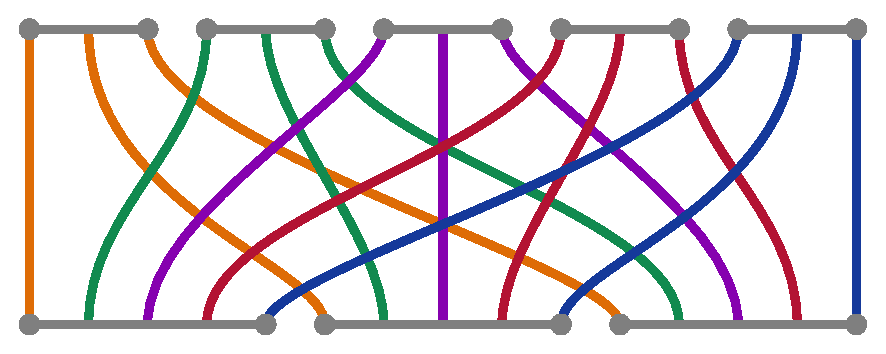
\includegraphics[width=0.8\columnwidth]{4-monoidal_structures/t-5-3.pdf}
\end{figure}
% We now give sufficient conditions for equipping the $2$-monad $\underline{P}$ associated to a $\Lambda$-operad $P$ with a pseudo-commutative structure. Let $\mathbb{N}_{+}$ denote the set of positive natural numbers.

We now define what it means for a $\Lambda$-operad to be pseudo-commuative, before then showing that such an operad yields a pseudo-commutative structure on the corresponding $2$-monad $\underline{P}$. Let $\mathbb{N}_{+}$ denote the set of positive integers.

QQQ Rewrite all this using the beta and delta operations, so it's consistent with before.
\begin{Defi}\label{def:ps-comm_operad}
Let $P$ be a $\Lambda$-operad. A pseudo-commutative structure on $P$ consists of:
    \begin{itemize}
        \item For each pair $(m,n) \in \mathbb{N}_{+}^2$, an element $t_{m,n} \in \Lambda(mn)$ such that $\pi(t_{m,n}) = \tau_{m,n}$.
        \item For each $p \in P(n)$, $q \in P(m)$, a natural isomorphism
            \[
                \lambda_{p,q} \colon \mu(p;q,\ldots,q) \cdot t_{m,n} \cong \mu(q;p,\ldots,p).
            \]
            We write this as $\lambda_{p,q}\colon \mu(p; \underline{q}) \cdot t_{m,n} \cong \mu(q; \underline{p})$.
    \end{itemize}
These are required to satisfy the following axioms:  
    \begin{enumerate}
        \item\label{axiom:t_id} For all $n \in \mathbb{N}_+$,
            \[
                t_{1,n} = e_n = t_{n,1}
            \]
             and for all $p \in P(n)$, the isomorphism $\lambda_{p, \id}\colon p \cdot e_n \cong p$ is the identity map.
        % \item\label{axiom:t_equiv} QQQ Equivariance axiom - we decided this was just naturality in the end! (See Remark 11.2 in \cite{guillou_multiplicative}.) QQQ It's basically `compose, act, switch' is the same as `compose, switch, act', but can't actually see where it's used in the proof:
        %   \[
        %     \lambda_{p \cdot g, q \cdot h} \circ \mu^P\left(\id_p \cdot g; \underline{\id_q \cdot h}\right) = \mu^P\left(\id_q \cdot h; \underline{\id_p \cdot g}\right) \circ \lambda_{p,q}.
        %   \]
        % For each $p \in P(n)$, $q \in P(m)$, $g \in \Lambda(n)$, and $h \in \Lambda(m)$, the following diagram commutes:
        %   \[
        %     \xy
        %       (-20,10)*+{\mu^P\left(p;\underline{q}\right) \cdot t_{m,n}}="a";
        %       (20,10)*+{\mu^P\left(q;\underline{p}\right)}="b";
        %       (-20,-10)*+{\mu^P\left(p \cdot g; \underline{q \cdot h}\right) \cdot t_{m,n}}="c";
        %       (20,-10)*+{\mu^P\left(q \cdot h; \underline{p \cdot g}\right)}="d";
        %       %
        %       {\ar^{\lambda_{p,q}} "a" ; "b"};
        %       {\ar^{\mu^P\left(\id_q \cdot h; \underline{\id_p \cdot g}\right)} "b" ; "d"};
        %       {\ar_{\mu^P\left(\id_p \cdot g; \underline{\id_q \cdot h}\right) \cdot t_{m,n}} "a" ; "c"};
        %       {\ar_{\lambda_{p \cdot g, q \cdot h}} "c" ; "d"};
        %     \endxy
        %   \]
        \item\label{axiom:t_sumR} For all $l, m_1, \ldots, m_l, n \in \mathbb{N}_+$, with $M = \Sigma m_i$,
            \[
                \mu^{\Lambda}\left(e_l; t_{m_1,n}, \ldots, t_{m_l,n}\right) \cdot \mu^{\Lambda}\left(t_{l,n};\underline{e_{m_1},\ldots,e_{m_l}}\right) = t_{n,M}.
            \]
            QQQ New version:
            \[
              \beta(t_{n,m_1},\ldots,t_{n,m_l}) \cdot \delta_{\underline{m_i},\ldots,\underline{m_i}}(t_{n,l}) = t_{n,M}.
            \]
            Here $\underline{e_{m_1},\ldots,e_{m_l}}$ is the list $e_{m_{1}}, \ldots, e_{m_{l}}$ repeated $n$ times.
        \item\label{axiom:t_sumL} For all $l, m, n_1,\ldots, n_m \in \mathbb{N}_+$, with $N = \Sigma n_i$,
            \[
                \mu^{\Lambda}\left(t_{m,l};\underline{e_{n_1}},\ldots,\underline{e_{n_m}}\right) \cdot \mu^{\Lambda}\left(e_m;t_{n_1,l},\ldots,t_{n_m,l}\right) = t_{N,l}.
            \]
            QQQ New version
            \[
              \delta_{\underline{n_1},\ldots,\underline{n_m}}(t_{m,l}) \cdot \beta(t_{n_1,l},\ldots,t_{n_m,l}) = t_{N,l}.
            \]
            Here $\underline{e_{n_{i}}}$ indicates that each $e_{n_{i}}$ is repeated $l$ times.
        \item\label{axiom:t_diagR} For any $l, m_i, n \in \mathbb{N}_+$, with $1 \leq i \leq n$, and $p \in P(l)$, $q_i \in P(m_i)$ and $r \in P(n)$, the following diagram commutes. (Note that we maintain the convention that anything underlined indicates a list, and double underlining indicates a list of lists. Each instance should have an obvious meaning from context and the equations appearing above.)
          \[
            \xy
                (0,0)*+{\mu\left(p;\underline{\mu(q_i;\underline{r})}\right) \cdot \mu(e_l;\underline{t_{n,m_i}})\mu(t_{n,l};\underline{\underline{e_{m_i}}})}="00";
                (60,0)*+{\mu\left(p;\underline{\mu(q_i;\underline{r})}\right) \cdot t_{n,M}}="10";
                (0,-15)*+{\mu\left(p;\underline{\mu(q_i;\underline{r})\cdot t_{n,m_i}}\right) \cdot \mu(t_{n,l};\underline{e_{m_1},\ldots,e_{m_l}})}="01";
                (60,-20)*+{\mu\left(\mu(p;q_1,\ldots,q_n);\underline{\underline{r}}\right)\cdot t_{n,M}}="11";
                (0,-30)*+{\mu\left(p;\underline{\mu(r;\underline{q_i})}\right) \cdot \mu(t_{n,l};\underline{e_{m_1},\ldots,e_{m_l}})}="02";
                (60,-40)*+{\mu\left(\mu(p;q_1,\ldots,q_n);\underline{\underline{r}}\right)}="12";
                (0,-45)*+{\mu\left(\mu(p;\underline{r}) \cdot t_{n,l} ; \underline{q_1,\ldots,q_n}\right)}="03";
                (60,-60)*+{\mu\left(r;\underline{\mu(p;q_1,\ldots,q_n)}\right)}="13";
                (0,-60)*+{\mu\left(\mu(r;\underline{p});\underline{q_1,\ldots,q_n}\right)}="04";
                {\ar@{=} "00" ; "10"};
                {\ar@{=} "00" ; "01"};
                {\ar@{=} "10" ; "11"};
                {\ar_{\mu(1;\underline{\lambda_{q_i,r}}) \cdot 1} "01" ; "02"};
                {\ar@{=} "02" ; "03"};
                {\ar@{=} "04" ; "13"};
                {\ar_{\mu(\lambda_{p,r};1)} "03" ; "04"};
                {\ar^{\lambda_{\mu(p;q_1,\ldots,q_n),r}} "11" ; "12"};
                {\ar@{=} "12" ; "13"};
            \endxy
          \]
        \item\label{axiom:t_diagL} For any $l,m, n_i \in \mathbb{N}_+$, with $1 \leq i \leq m$, and $p \in P(l)$, $q \in P(m)$ and $r_i \in P(n_i)$, the following diagram commutes.
          \[
            \xy
                (0,0)*+{\mu\left(\mu(p;\underline{q}) \cdot t_{m,l} ; \underline{\underline{r_i}}\right) \cdot \mu(e_m;\underline{t_{n_i,l}})}="00";
                (60,0)*+{\mu\left(\mu(p;\underline{q});\underline{\underline{r_i}}\right) \cdot \mu(t_{m,l};\underline{\underline{e_{n_i}}})\mu(e_{m};\underline{t_{n_i,l}})}="10";
                (60,-15)*+{\mu\left(p;\underline{\mu(q;\underline{r_i})}\right) \cdot \mu(t_{m,l};\underline{\underline{e_{n_i}}})\mu(e_{m};\underline{t_{n_i,l}})}="11";
                (0,-20)*+{\mu\left(\mu(q;\underline{p}); \underline{r_1},\ldots,\underline{r_m}\right) \cdot \mu(e_m;\underline{t_{n_i,l}})}="01";
                (0,-40)*+{\mu\left(q;\underline{\underline{\mu(p;r_i)}}\right) \cdot \mu(e_m;\underline{t_{n_i,l}})}="02";
                (0,-60)*+{\mu\left(q;\underline{\mu(p;\underline{r_i}) \cdot t_{n_i,l}}\right)}="03";
                (60,-30)*+{\mu\left(p;\underline{\mu(q;r_1,\ldots,r_m)}\right) \cdot t_{N,l}}="12";
                (60,-45)*+{\mu\left(\mu(q;r_1,\ldots,r_m); \underline{\underline{p}}\right)}="13";
                (60,-60)*+{\mu\left(q;\underline{\mu(r_i;\underline{p})}\right)}="14";
                {\ar@{=} "00" ; "10"};
                {\ar@{=} "10" ; "11"};
                {\ar@{=} "11" ; "12"};
                {\ar^{\lambda_{p,\mu(q;r_1,\ldots,r_m)}} "12" ; "13"};
                {\ar@{=} "13" ; "14"};
                {\ar_{\mu(\lambda_{p,q};1) \cdot 1} "00" ; "01"};
                {\ar@{=} "01" ; "02"};
                {\ar@{=} "02" ; "03"};
                {\ar_{\mu(1;\underline{\lambda_{p,r_i}})} "03" ; "14"};
            \endxy
          \]
    \end{enumerate}
\end{Defi}

\begin{remark}
Remark 11.2 of \cite{guillou_multiplicative} describes the need for an extra equivariance axiom in the pseudo-commutative structure definition, some detail of which is also described in \cite{guillou_symmetric}. We also believed this to be true until a realisation that the equivariance axiom of \cite{guillou_multiplicative}[11.1, Axiom (iii)] becomes the following requirement:
          \[
            \lambda_{p \cdot g, q \cdot h} \circ \left(\mu^P\left(\id_p \cdot g; \underline{\id_q \cdot h}\right) \cdot t_{m,n}\right) = \mu^P\left(\id_q \cdot h; \underline{\id_p \cdot g}\right) \circ \lambda_{p,q}.
          \]
On closer inspection, this appears to be an instance of naturality for the natural isomorphisms $\lambda$, as shown in the naturality square below.
          \[
            \xy
              (-20,10)*+{\mu^P\left(p;\underline{q}\right) \cdot t_{m,n}}="a";
              (20,10)*+{\mu^P\left(q;\underline{p}\right)}="b";
              (-20,-10)*+{\mu^P\left(p \cdot g; \underline{q \cdot h}\right) \cdot t_{m,n}}="c";
              (20,-10)*+{\mu^P\left(q \cdot h; \underline{p \cdot g}\right)}="d";
              %
              {\ar^{\lambda_{p,q}} "a" ; "b"};
              {\ar^{\mu^P\left(\id_q \cdot h; \underline{\id_p \cdot g}\right)} "b" ; "d"};
              {\ar_{\mu^P\left(\id_p \cdot g; \underline{\id_q \cdot h}\right) \cdot t_{m,n}} "a" ; "c"};
              {\ar_{\lambda_{p \cdot g, q \cdot h}} "c" ; "d"};
            \endxy
          \]
\end{remark}

\begin{thm}\label{pscomm}
Let $P$ be a $\Lambda$-operad equipped with a pseudo-commutative structure. Then $\underline{P}$ has a pseudo-commutativity.
\end{thm}

% \begin{thm}\label{pscomm}
% Let $P$ be a $\Lambda$-operad. Then the following equip $\underline{P}$ with a pseudo-commutative structure.
%     \begin{itemize}
%         \item For each pair $(m,n) \in \mathbb{N}_{+}^2$, we are given an element $t_{m,n} \in \Lambda(mn)$ such that $\pi(t_{m,n}) = \tau_{m,n}$.
%         \item For each $p \in P(n)$, $q \in P(m)$, we are given a natural isomorphism
%             \[
%                 \lambda_{p,q} \colon \mu(p;q,\ldots,q) \cdot t_{m,n} \cong \mu(q;p,\ldots,p).
%             \]
%             We write this as $\lambda_{p,q}\colon \mu(p; \underline{q}) \cdot t_{m,n} \cong \mu(q; \underline{p})$.
%     \end{itemize}
% These must satisfy the following:  
%     \begin{enumerate}
%         \item For all $n \in \mathbb{N}_+$\nomenclature[N]{$\mathbb{N}_+$}{the set of positive natural numbers},
%             \[
%                 t_{1,n} = e_n = t_{n,1}
%             \]
%              and for all $p \in P(n)$, the isomorphism $\lambda_{p, \id}\colon p \cdot e_n \cong p$ is the identity map.
%         \item For all $l, m_1, \ldots, m_l, n \in \mathbb{N}_+$, with $M = \Sigma m_i$,
%             \[
%                 \mu^{\Lambda}\left(e_l; t_{m_1,n}, \ldots, t_{m_l,n}\right) \cdot \mu^{\Lambda}\left(t_{l,n};\underline{e_{m_1},\ldots,e_{m_l}}\right) = t_{n,M}.
%             \]
%             Here $\underline{e_{m_1},\ldots,e_{m_l}}$ is the list $e_{m_{1}}, \ldots, e_{m_{l}}$ repeated $n$ times.
%         \item For all $l, m, n_1,\ldots, n_m \in \mathbb{N}_+$, with $N = \Sigma n_i$,
%             \[
%                 \mu^{\Lambda}\left(t_{m,l};\underline{e_{n_1}},\ldots,\underline{e_{n_m}}\right) \cdot \mu^{\Lambda}\left(e_m;t_{n_1,l},\ldots,t_{n_m,l}\right) = t_{N,l}.
%             \]
%             Here $\underline{e_{n_{i}}}$ indicates that each $e_{n_{i}}$ is repeated $l$ times.
%         \item For any $l, m_i, n \in \mathbb{N}_+$, with $1 \leq i \leq n$, and $p \in P(l)$, $q_i \in P(m_i)$ and $r \in P(n)$, the following diagram commutes. (Note that we maintain the convention that anything underlined indicates a list, and double underlining indicates a list of lists. Each instance should have an obvious meaning from context and the equations appearing above.)
%           \[
%             \xy
%                 (0,0)*+{\mu\left(p;\underline{\mu(q_i;\underline{r})}\right) \cdot \mu(e_l;\underline{t_{n,m_i}})\mu(t_{n,l};\underline{\underline{e_{m_i}}})}="00";
%                 (60,0)*+{\mu\left(p;\underline{\mu(q_i;\underline{r})}\right) \cdot t_{n,M}}="10";
%                 (0,-15)*+{\mu\left(p;\underline{\mu(q_i;\underline{r})\cdot t_{n,m_i}}\right) \cdot \mu(t_{n,l};\underline{e_{m_1},\ldots,e_{m_l}})}="01";
%                 (60,-20)*+{\mu\left(\mu(p;q_1,\ldots,q_n);\underline{\underline{r}}\right)\cdot t_{n,M}}="11";
%                 (0,-30)*+{\mu\left(p;\underline{\mu(r;\underline{q_i})}\right) \cdot \mu(t_{n,l};\underline{e_{m_1},\ldots,e_{m_l}})}="02";
%                 (60,-40)*+{\mu\left(\mu(p;q_1,\ldots,q_n);\underline{\underline{r}}\right)}="12";
%                 (0,-45)*+{\mu\left(\mu(p;\underline{r}) \cdot t_{n,l} ; \underline{q_1,\ldots,q_n}\right)}="03";
%                 (60,-60)*+{\mu\left(r;\underline{\mu(p;q_1,\ldots,q_n)}\right)}="13";
%                 (0,-60)*+{\mu\left(\mu(r,\underline{p});\underline{q_1,\ldots,q_n}\right)}="04";
%                 {\ar@{=} "00" ; "10"};
%                 {\ar@{=} "00" ; "01"};
%                 {\ar@{=} "10" ; "11"};
%                 {\ar_{\mu(1;\underline{\lambda_{q_i,r}}) \cdot 1} "01" ; "02"};
%                 {\ar@{=} "02" ; "03"};
%                 {\ar@{=} "04" ; "13"};
%                 {\ar_{\mu(\lambda_{p,r};1)} "03" ; "04"};
%                 {\ar^{\lambda_{\mu(p;q_1,\ldots,q_n),r}} "11" ; "12"};
%                 {\ar@{=} "12" ; "13"};
%             \endxy
%           \]
%         \item For any $l,m, n_i \in \mathbb{N}_+$, with $1 \leq i \leq m$, and $p \in P(l)$, $q \in P(m)$ and $r_i \in P(n_i)$, the following diagram commutes.
%           \[
%             \xy
%                 (0,0)*+{\mu\left(\mu(p;\underline{q}) \cdot t_{m,l} ; \underline{\underline{r_i}}\right) \cdot \mu(e_m;\underline{t_{n_i,l}})}="00";
%                 (60,0)*+{\mu\left(\mu(p;\underline{q});\underline{\underline{r_i}}\right) \cdot \mu(t_{m,l};\underline{\underline{e_{n_i}}})\mu(e_{m};\underline{t_{n_i,l}})}="10";
%                 (60,-15)*+{\mu\left(p;\underline{\mu(q;\underline{r_i})}\right) \cdot \mu(t_{m,l};\underline{\underline{e_{n_i}}})\mu(e_{m};\underline{t_{n_i,l}})}="11";
%                 (0,-20)*+{\mu\left(\mu(q;\underline{p}); \underline{r_1},\ldots,\underline{r_m}\right) \cdot \mu(e_m;\underline{t_{n_i,l}})}="01";
%                 (0,-40)*+{\mu\left(q;\underline{\underline{\mu(p;r_i)}}\right) \cdot \mu(e_m;\underline{t_{n_i,l}})}="02";
%                 (0,-60)*+{\mu\left(q;\underline{\mu(p;\underline{r_i}) \cdot t_{n_i,l}}\right)}="03";
%                 (60,-30)*+{\mu\left(p;\underline{\mu(q;r_1,\ldots,r_m)}\right) \cdot t_{N,l}}="12";
%                 (60,-45)*+{\mu\left(\mu(q;r_1,\ldots,r_m); \underline{\underline{p}}\right)}="13";
%                 (60,-60)*+{\mu\left(q;\underline{\mu(r_i;\underline{p})}\right)}="14";
%                 {\ar@{=} "00" ; "10"};
%                 {\ar@{=} "10" ; "11"};
%                 {\ar@{=} "11" ; "12"};
%                 {\ar^{\lambda_{p,\mu(q;r_1,\ldots,r_m)}} "12" ; "13"};
%                 {\ar@{=} "13" ; "14"};
%                 {\ar_{\mu(\lambda_{p,q};1) \cdot 1} "00" ; "01"};
%                 {\ar@{=} "01" ; "02"};
%                 {\ar@{=} "02" ; "03"};
%                 {\ar_{\mu(1;\underline{\lambda_{p,r_i}})} "03" ; "14"};
%             \endxy
%           \]
%     \end{enumerate}
% \end{thm}

\begin{proof}
We refer to the Axioms in \cref{def:ps-comm_operad} throughout. We begin the proof by defining an invertible modification $\gamma$ for the pseudo-commutativity for which the components are natural transformations $\gamma_{A,B}$. Such a transformation $\gamma_{A,B}$ has components with source
  \[
    \left[\mu\left(p; \underline{q}\right); \underline{(a, \underline{b})}\right]
  \]
and target
  \[
    \left[\mu\left(q; \underline{p}\right); \underline{(\underline{a},b)}\right].
  \]
Now $ \lambda_{p,q} \colon \mu(p;q,\ldots,q) \cdot t_{m,n} \cong \mu(q;p,\ldots,p)$ gives rise to another map by multiplication on the right by $t_{m,n}^{-1}$,
  \[
    \lambda_{p,q}\cdot t_{m,n}^{-1} \colon \mu(p;q,\ldots,q) \cong \mu(q;p,\ldots,p) \cdot t_{m,n}^{-1},
  \]
so we define $(\gamma_{A,B})_{[p;a_1,\ldots,a_n],[q;b_1,\ldots,b_m]}$ to be the morphism which is the image of $(\lambda_{p,q}\cdot t_{m,n}^{-1}, 1)$ under the map
  \[
    \coprod P(n) \times (A \times B)^{n} \rightarrow \coprod \coeq{P}{A \times B}{\Lambda}{n}.
  \]
Naturality of $\gamma_{A,B}$ follows from that of each $\lambda_{p,q}$. We will write this morphism as $[\lambda_{p,q}t_{m,n}^{-1}, 1]$. In the case that either $p$ or $q$ is an identity then we choose the component of $\gamma$ to be the isomorphism involving the appropriate identity element using Axiom \ref{axiom:t_id} above.

There are two things to note about the definition above before we continue. First, it is easy to check that
  \[
    t_{m,n}^{-1} \cdot \underline{\left(a, \underline{b}\right)} = \underline{\left(\underline{a},b\right)}
  \]
since $\pi(t_{m,n}) = \tau_{m,n}$; this ensures that $\gamma$ has the correct target. Second, the morphism above has second component the identity. This is actually forced upon us by the requirement that $\gamma$ be a modification:  in the case that $A,B$ are discrete categories, the only possible morphism is an identity, and the modification axiom then forces that statement to be true for general $A,B$ by considering the inclusion $A_{0} \times B_{0} \hookrightarrow A \times B$ where $A_{0}, B_{0}$ are the discrete categories with the same objects as $A, B$.

We show that this is a modification by noting that it does not rely on objects in the lists $a_1, \ldots, a_n$ or $b_1, \ldots, b_m$, only on their lengths and the operations $p$ and $q$. As a result, if there are functors $f \colon A \rightarrow A'$ and $g \colon B \rightarrow B'$, then it is clear that
    \[
        (\underline{P}(f\times g) \circ \gamma_{A,B})_{\left[p;\underline{a}\right],\left[q;\underline{b}\right]} = [\lambda_{p,q},\underline{1}] = (\gamma_{A',B'} \circ (\underline{P}f\times \underline{P}g))_{\left[p;\underline{a}\right],\left[q;\underline{b}\right]}.
    \]
As such we can simply write $(\gamma_{A,B})_{[p;\underline{a}],[q;\underline{b}]}$ in shorthand as $\gamma_{p,q}$.

There are now seven axioms to check for a pseudo-commutativity:  three strength axioms, two unit axioms, and two multiplication axioms. For the first strength axiom, we must verify that two different $2$-cells of shape
  \[
    \xy
      (0,0)*+{A \times TB \times TC}="0";
      (50,0)*+{T(A \times B \times C)}="1";
      {\ar@/^1pc/ "0"; "1"};
      {\ar@/_1pc/ "0"; "1"};
      (25,0)*{\Downarrow}
    \endxy
  \]
are equal. The first of these is $\gamma$ precomposed with $d \times 1$, and so is the component of $\gamma$ at an object
  \[
    \left( [p;(a,b_1),\ldots,(a,b_n)], [q; c_{1}, \ldots, c_{m}] \right).
  \]
The second of these is $d$ applied to the component of $1 \times \gamma$ at
  \[
    \left(a, ([p;b_1,\ldots,b_n], [q; c_{1}, \ldots, c_{m}]) \right).
  \]
It is straightforward to compute that each of these maps is the image of $\left(\lambda_{p,q}\cdot t_{m,n}^{-1},1\right)$ under the functor
  \[
    \coprod P(n) \times (A \times B)^{n} \rightarrow \coprod \coeq{P}{A \times B}{\Lambda}{n}.
  \]
The other two strength axioms follow by analogous calculations for other whiskerings of $\gamma$ with $d$ or $d^{*}$.

For the unit axioms, we must compute the components of $\gamma$ precomposed with $\eta \times 1$ for the first axiom and $1 \times \eta$ for the second. Thus for the first unit axiom, we must compute the component of $\gamma$ at $\left( [e;a], [p; b_{1}, \ldots, b_{m}] \right)$. By definition, this is the image of $(\lambda_{e,p}\cdot t^{-1}_{m,1}, 1)$ under the map to the coequalizer, and by Axiom \ref{axiom:t_id} of \ref{def:ps-comm_operad} know that $t^{-1}_{m,1}$ is the identity element and this isomorphism is the identity as well, so this component of $\gamma$ is also the identity. The second unit axiom follows similarly, using that $t^{-1}_{1,n}$ is the identity.

For the multiplication axioms, first note that Axiom \ref{axiom:t_sumR} is necessary in order to ensure the existence of the top horizontal equality in the diagram of Axiom \ref{axiom:t_diagR} for the pseudo-commutative structure; the same goes for Axioms \ref{axiom:t_sumL} and \ref{axiom:t_diagL}. We now explain how Axioms \ref{axiom:t_sumR} and \ref{axiom:t_diagR} for the pseudo-commutative structure ensure that the first multiplication axiom holds, with the same reasoning showing that Axioms \ref{axiom:t_sumL} and \ref{axiom:t_diagL} imply the second multiplication axiom.

We begin by studying the pasting diagram in the first multiplication axiom, but computing its values using the strength and costrength for the non-symmetric operad underlying $P$; this means that we evaluate on objects of the form $(p; a_{1}, \ldots, a_{n})$ rather than on their equivalence classes. Let $p \in P(l), q_{i} \in P(m_{i})$ for $1 \leq i \leq l$, and $r \in P(n)$. Computing the top and right leg around the pasting diagram gives the function on objects which sends
  \[
    \left( (p; (q_{1}; \un{a_{1}}), \ldots, (q_{l}; \un{a_{l}})), (r; \un{b}) \right)
  \]
to
  \[
    \left( \mu(p; \mu(q_{1}; \un{r}), \ldots, \mu(q_{l}; \un{r})); (\un{(a_{1\bullet}, \un{b})}), \ldots, (\un{(a_{l\bullet}, \un{b})}) \right),
  \]
where $(\un{(a_{i\bullet}, \un{b})})$ is the list of pairs
  \[
    (a_{i1}, b_{1}), \ldots, (a_{i1}, b_{m}), (a_{i2}, b_{1}), \ldots, (a_{in_{i}}, b_{m}).
  \]
Then $\un{P}\gamma$ is the image of the morphism which is the identity on the $(a_{ij}, b_{k})$'s, and is the morphism
  \[
    \mu\left(1;\lambda_{q_1,r}t^{-1}_{n,m_1},\ldots,\lambda_{q_l,r}t^{-1}_{n,m_l}\right)
  \]
on the first component with domain and codomain shown below.
  \[
    \mu\left(p;\mu\left(q_1;\un{r}\right),\ldots,\mu\left(q_n;\un{r}\right)\right) \longrightarrow \mu\left(p;\mu\left(r;\un{q_1}\right)t^{-1}_{n,m_1},\ldots,\mu\left(r;\un{q_l}\right)t^{-1}_{n,m_l}\right)
  \]
% \[
% \xy
% {\ar^{\scriptstyle \mu\left(1; \lambda_{q_{1}, r} t^{-1}_{n,m_{1}}, \ldots, \lambda_{q_{1}, r} t^{-1}_{n,m_{l}}\right)} (0,0)*+{\scriptstyle \mu\left(p; \mu(q_{1}; \un{r}), \ldots, \mu(q_{n}; \un{r})\right)}; (75,0)*+{\scriptstyle \mu\left(p; \mu(r; \un{q_{1}}) t^{-1}_{n,m_{1}}, \ldots, \mu(r; \un{q_{l}}) t^{-1}_{n,m_{l}} \right)} }
% \endxy
% \]
% on the first component. 
By the $\Lambda$-operad axioms, the target of this morphism is equal to
  \[
    \mu\left(p; \mu\left(r; \un{q_{1}}\right), \ldots, \mu\left(r; \un{q_{l}}\right) \right)\mu\left(e_{l}; t^{-1}_{n,m_{1}}, \ldots, t^{-1}_{n,m_{l}}\right).
  \]
Note that this is not the same object as one obtains by computing $T\mu \circ T^{2}d^{*} \circ Td \circ d^{*}$ using the underlying non-symmetric operad of $P$ as we are required to use the $\Lambda$-equivariance to ensure that the target of $\gamma$ is the correct one.

Next we compute the source of $(\mu \circ Td^{*})*\gamma$, the other $2$-cell in the pasting appearing in the first multiplication axiom. We compute this once again using the strength and costrength for the underlying non-symmetric operad, and note once again that this will not match our previous calculations precisely, but only up to an application of $\Lambda$-equivariance. This functor has its map on objects given by
  \[
    \left( (p; (q_{1}; \un{a_{1}}), \ldots, (q_{l}; \un{a_{l}})), (r; \un{b}) \right) \mapsto \left(\mu(\mu(p; \un{r}); \un{q_{1}}, \ldots, \un{q_{l}}); \un{(\un{a_{1}}, b_{\bullet})}, \ldots, \un{(\un{a_{l}}, b_{\bullet})} \right).
  \]
  Note that if we apply $\Lambda$-equivariance, this matches the target computed above. Once again the component of $\gamma$ is the image of a morphism which is the identity on the $(a_{ij}, b_{k})$'s, and its first component is
  \[
    \xy
      {\ar^{\mu\left(\lambda_{p,r} \cdot t^{-1}_{n,l}; 1, \ldots, 1\right)} (0,0)*+{\mu\left(\mu(p; \un{r}); \un{q_{1}}, \ldots, \un{q_{l}}\right)}; (60,0)*+{\mu\left(\mu(r; \un{p})\cdot t^{-1}_{n,l}; \un{q_{1}}, \ldots, \un{q_{l}}\right).} }
    \endxy
  \]

We cannot compose these morphisms in $\coprod P(n) \times (A \times B)^{n}$ as they do not have matching source and target, but we can in $\coprod P(n) \times_{\Lambda} (A \times B)^{n}$. The resulting morphism has first component given by the image of
  \[
    \xy
      {\ar^{\scriptstyle \mu\left(1; \lambda_{q_{1}, r} t^{-1}_{n,m_{1}}, \ldots, \lambda_{q_{1}, r} t^{-1}_{n,m_{l}}\right)} (0,0)*+{\scriptstyle \mu\left(p; \mu\left(q_{1}; \un{r}\right), \ldots, \mu\left(q_{n}; \un{r}\right)\right)}; (75,0)*+{\scriptstyle \mu\left(p; \mu\left(r; \un{q_{1}}\right) t^{-1}_{n,m_{1}}, \ldots, \mu\left(r; \un{q_{l}}\right) t^{-1}_{n,m_{l}} \right)} };
      {\ar^<<<<<<<<<<<<<<<<<<<<<<{\scriptstyle \mu\left(\lambda_{p,r} \cdot t^{-1}_{n,l}; 1, \ldots, 1\right)\cdot \mu\left(e_{l}; t^{-1}_{n,m_{1}}, \ldots, t^{-1}_{n,m_{l}}\right)} (0,-10)*+{}; (75,-10)*+{\scriptstyle \mu\left(\mu\left(r; \un{p}\right)\cdot t^{-1}_{n,l}; \un{q_{1}}, \ldots, \un{q_{l}}\right)\cdot \mu\left(e_{l}; t^{-1}_{n,m_{1}}, \ldots, t^{-1}_{n,m_{l}}\right),} }
    \endxy
  \]
where we have made use of the operad axioms in identifying the target of the first map with the source of the second. Using the $\Lambda$-operad axioms again on the target, we find that
  \[
    \mu\left(\mu(r; \un{p})\cdot t^{-1}_{n,l}; \un{q_{1}}, \ldots, \un{q_{l}}\right)\cdot \mu(e_{l}; t^{-1}_{n,m_{1}}, \ldots, t^{-1}_{n,m_{l}})
  \]
is equal to
  \[
    \mu\left(\mu(r; \un{p}); \un{q_{1}, \ldots, q_{l}}\right) \cdot \mu(t^{-1}_{n,l}; \un{e}) \cdot \mu(e_{l}; t^{-1}_{n,m_{1}}, \ldots, t^{-1}_{n,m_{l}}).
  \]
This composite of two morphisms, together with the necessary identities coming from operad axioms, is precisely the left and bottom leg of the diagram in Axiom \ref{axiom:t_diagR}. Using the same method, one then verifies that $\gamma * (\mu \times 1)$ has its first component the image of the morphism appearing along the top and right leg of the diagram in \ref{axiom:t_diagR}. The second component of these morphisms are all identities arising from $\Lambda$-equivariance, so the first multiplication axiom is a consequence of Axioms \ref{axiom:t_sumR} and \ref{axiom:t_diagR} for the pseudo-commutative structure. We leave the calculations for the second multiplication axiom to the reader as they are of the same nature, using Axioms \ref{axiom:t_sumL} and \ref{axiom:t_diagL}.
\end{proof}

\begin{cor}
Let $P$ be a non-symmetric operad. Then the induced monad $\underline{P}$ is never pseudo-commutative.
\end{cor}
\begin{proof}
In the non-symmetric case, the $2$-monad is just given using coproducts and products, i.e., there is no coequalizer. In order to define $\gamma$, we then need an isomorphism
  \[
    \left(\mu(p; \underline{q}); \underline{(a, \underline{b})}\right) \cong \left(\mu(q; \underline{p}); \underline{(\underline{a},b)}\right).
  \]
When $A,B$ are discrete, there is no isomorphism $\underline{\left(a,\underline{b}\right)} \cong \underline{\left(\underline{a},b\right)}$, and therefore no such $\gamma$ can exist.
\end{proof}



A further property that a pseudo-commutativity can possess is that of symmetry. This symmetry is then reflected in the monoidal structure on the $2$-category of algebras, which will then also have a symmetric tensor product (in a suitable, $2$-categorical sense).

\begin{Defi}
Let $T \colon \m{K} \rightarrow \m{K}$ be a $2$-monad on a symmetric monoidal $2$-category $\m{K}$ with symmetry $c$. We then say that a pseudo-commutativity $\gamma$ for $T$ is \textit{symmetric} when the following is satisfied for all $A$, $B \in \m{K}$:
    \[
        Tc_{A,B} \circ \gamma_{A,B} \circ c_{TB, TA} = \gamma_{B,A}.
    \]
\end{Defi}

With the notion of symmetry at hand we are able to extend the above theorem, stating when $\underline{P}$ is symmetric.
\begin{thm}
The pseudo-commutativity of $\underline{P}$ given by \cref{pscomm}  is symmetric if for all $m,n \in \mathbb{N}_+$ the two conditions below hold.
    \begin{enumerate}
        \item $t_{m,n} = t_{n,m}^{-1}$.
        \item The following diagram commutes:
          \[
              \xy
                (0,0)*+{\mu\left(p;\underline{q}\right) \cdot t_{m,n}t_{n,m}}="00";
                (30,0)*+{\mu\left(p;\underline{q}\right) \cdot e_{mn}}="10";
                (0,-15)*+{\mu\left(q;\underline{p}\right) \cdot t_{n,m}}="01";
                (30,-15)*+{\mu\left(p;\underline{q}\right)}="11";
                {\ar@{=} "00" ; "10"};
                {\ar_{\lambda_{p,q} \cdot 1} "00" ; "01"};
                {\ar@{=} "10" ; "11"};
                {\ar_{\lambda_{q,p}} "01" ; "11"};
              \endxy
          \]
    \end{enumerate}
\end{thm}
\begin{proof}
The commutativity of the diagram above ensures that the first component of the symmetry axiom commutes in $P(n)$ before taking equivalence classes in the coequalizer, just as in the proof of \cref{pscomm}.
\end{proof}

\begin{Defi}
Let $P$ be a $\Lambda$-operad in $\mb{Cat}$. We say that $P$ is \textit{contractible} if each category $P(n)$ is equivalent to the terminal category.
\end{Defi}

\begin{cor}
If $P$ is contractible and there exist $t_{m,n}$ as in \cref{pscomm}, then $\underline{P}$ acquires a pseudo-commutativity. Furthermore, it is symmetric if $t_{n,m} = t_{m,n}^{-1}$.
\end{cor}
\begin{proof}
The only thing left to define is the collection of natural isomorphisms $\lambda_{p,q}$. But since each $P(n)$ is contractible, $\lambda_{p,q}$ must be the unique isomorphism between its source and target, and furthermore the last two axioms hold since any pair of parallel arrows are equal in a contractible category.
\end{proof}

\begin{cor}
If $P$ is a contractible symmetric operad then $\underline{P}$ has a symmetric pseudo-commutativity.
\end{cor}
\begin{proof}
We choose $t_{m,n} = \tau_{m,n}$.
\end{proof}

\begin{rem}
If a $\Lambda$-operad $P$ is contractible, it is not the case that its symmetrization $S(P)$ (see \cref{thm_sym}) will also be contractible. The category $\coequ{P}{\Sigma}{\Lambda}{n}$ will necessarily be a groupoid as it is a colimit of groupoids: contractible categories are always groupoids, and both $\Lambda(n)$ and $\Sigma_{n}$ are discrete. Let $g \in \textrm{ker} \, \pi_{n}$ be any non-identity element, and let $p \in P(n)$ be any object. Then
  \[
    [p \cdot g, e] = [p, \pi(g)e] = [p,e],
  \]
but unless $p\cdot g = p$ in $P(n)$, there will be a unique isomorphism between them that will not be the identity, and hence will define a nontrivial automorphism of $[p,e]$ in  $\coequ{P}{\Sigma}{\Lambda}{n}$. The existence of such ensures that $\coequ{P}{\Sigma}{\Lambda}{n}$ is not contractible.
\end{rem}



\section{Extended Example: Coboundary Categories}\label{sec:exex-cactus}

We now turn to an example which is not as widely known in the categorical literature, that of coboundary categories \cite{drin-quasihopf}. These arise in the representation theory of quantum groups and in the theory of crystals \cite{hk-cobound, hk-quantum}. Our goal here is to refine the relationship between coboundary categories and the operad of $n$-fruit cactus groups in \cite{hk-cobound} by using the theory of action operads and our Borel construction. We begin by recalling the definition of a coboundary category.


\begin{Defi}\label{def:cobcat}
A \textit{coboundary category} is a monoidal category $C$ equipped with a natural isomorphism $\sigma_{x,y} \colon x \otimes y \rightarrow y \otimes x$ (called the \textit{commutor}) such that
\begin{itemize}
\item $\sigma_{y,x} \circ \sigma_{x,y} = 1_{x \otimes y}$ and
\item the diagram
  \[
    \xy
      (0,0)*+{(x \otimes y) \otimes z} ="00";
      (35,0)*+{x \otimes (y \otimes z)} ="10";
      (70,0)*+{x \otimes (z \otimes y)} ="20";
      (0,-15)*+{(y \otimes x) \otimes z} ="01";
      (35,-15)*+{z \otimes (y \otimes x)} ="11";
      (70,-15)*+{(z \otimes y )\otimes x} ="21";
      {\ar "00"; "10" };
      {\ar^{1 \sigma_{y,z}} "10"; "20" };
      {\ar^{\sigma_{x,zy}} "20"; "21" };
      {\ar_{\sigma_{x,y}1} "00"; "01" };
      {\ar_{\sigma_{yx,z}} "01"; "11" };
      {\ar "11"; "21" };
    \endxy
  \]
commutes (in which the unlabeled morphisms are an associator and an inverse associator).
\end{itemize}
\end{Defi}

\begin{example}\label{ex:cobcats}
\begin{enumerate}
\item As noted by Savage \cite{savage-braidcob}, any braiding automatically satisfies the cactus relation (the diagram in \cref{def:cobcat}). However, since braidings need not be involutions this does not mean that any braided monoidal category is a coboundary category. However, it should then be clear that any symmetric monoidal category is also a coboundary category.
\item The name coboundary category comes from the original work of Drinfeld \cite{drin-quasihopf} in which he shows that the category of representations of a coboundary Hopf algebra has the structure of coboundary category.
\item Henriques and Kamnitzer \cite{hk-cobound} show that the category of crystals for a finite dimensional complex reductive Lie algebra has the structure of a coboundary category. 
\end{enumerate}
\end{example}

Our interest is in strict coboundary categories by which we mean coboundary categories with strict underlying monoidal category. Under the assumption of strictness, the second axiom above does not include associations for the tensor product and reduces to a square. To show that every coboundary category is equivalent to a strict coboundary category, we must introduce the $2$-category $\mb{CobCat}$ of coboundary categories.

\begin{Defi}
Let $(C,\sigma), (C', \sigma')$ be coboundary categories. A \emph{coboundary functor} $F \colon C \rightarrow C'$ is a strong monoidal functor (with invertible constraints $\varphi_{0}$ for the unit and $\varphi_{x,y}$ for the tensor product) such that the following diagram commutes for all objects $x$, $y \in \m{C}$.
  \[
    \xy
      (0,0)*+{Fx \otimes Fy}="00";
      (25,0)*+{F(x \otimes y)}="10";
      (0,-20)*+{Fy \otimes Fx}="01";
      (25,-20)*+{F(y \otimes x)}="11";
      %
      {\ar^{\varphi_{x,y}} "00";"10"};
      {\ar^{F\sigma_{x,y}} "10";"11"};
      {\ar_{\sigma_{Fx,Fy}} "00";"01"};
      {\ar_{\varphi_{y,x}} "01";"11"};
    \endxy
  \]
  % \[
  %   F\sigma_{x,y} \circ \varphi_{x,y} = \varphi_{y,x} \circ \sigma_{Fx,Fy}'
  % \]
\end{Defi}

Coboundary functors are composed just as strong monoidal functors are, giving the following.

\begin{lem}
Coboundary categories, coboundary functors, and monoidal transformations form a $2$-category, which we denote $\mb{CobCat}$.
\end{lem}


\begin{prop}
Let $(C, \sigma)$ be a coboundary category. Then there exists a strict coboundary category $(C', \sigma')$ which is equivalent to $(C, \sigma)$ in $\mb{CobCat}$.
\end{prop}
\begin{proof}
Consider the underlying monoidal category of $(C, \sigma)$, which we will just write as $C$. We can find a strict monoidal category $C'$ by coherence for monoidal categories together with an equivalence, as monoidal categories, between $C$ and $C'$. By standard methods \cite{maclane-catwork}, this can be improved to an adjoint equivalence between $C$ and $C'$ in the $2$-category of monoidal categories, strong monoidal functors, and monoidal transformations. Let $F \colon  C \rightarrow C', G \colon C' \rightarrow C$ be the functors in this adjoint equivalence, and $\eta \colon 1 \Rightarrow FG$ the unit (which we note for emphasis is invertible since it the unit of an adjoint equivalence). For objects $x,y \in C'$, we define a commutor $\sigma'$ for $C'$ as the following composite.
  % \begin{align*}
  %   xy & \stackrel{\eta \otimes \eta}{\longrightarrow} FGxFGy \\
  %   & \stackrel{\cong}{\longrightarrow} F(GxGy) \\
  %   & \stackrel{F\sigma}{\longrightarrow} F(GyGx) \\
  %   & \stackrel{\cong}{\longrightarrow}  FGyFGx \\
  %   & \stackrel{\eta^{-1} \otimes \eta^{-1}}{\longrightarrow} yx.
  % \end{align*}
  % \begin{align*}
  %   xy &\xrightarrow{\eta \otimes \eta} FGxFGy \\
  %   &\xrightarrow{\cong} F(GxGy) \\
  %   &\xrightarrow{F\sigma} F(GyGx) \\
  %   &\xrightarrow{\cong} FGyFGx \\
  %   &\xrightarrow{\eta^{-1} \otimes \eta^{-1}} yx
  % \end{align*}
  \[
    xy \xrightarrow{\eta \otimes \eta} FGxFGy
    \xrightarrow{\cong} F(GxGy)
    \xrightarrow{F\sigma} F(GyGx)
    \xrightarrow{\cong} FGyFGx
    \xrightarrow{\eta^{-1} \otimes \eta^{-1}} yx
  \]
We then leave to the reader, if they wish, the computations to show that $\sigma'$ is a commutor for $C'$ and that $F,G$ become coboundary functors using $\sigma'$.
\end{proof}

We now turn to the operadic description of strict coboundary categories; we note from this point onwards, all our coboundary categories are assumed to be strict.

\begin{Defi}
Fix $n>1$, and let $1 \leq p < q \leq n$, $1 \leq k < l \leq n$.
\begin{enumerate}
\item $p<q$ is \textit{disjoint} from $k<l$ if $q<k$ or $l<p$.
\item $p<q$ \textit{contains} $k<l$ if $p \leq k < l \leq q$.
\end{enumerate}
\end{Defi}

\begin{Defi}
Let $1 \leq p < q \leq n$, and define $\hat{s}_{p,q} \in \Sigma_{n}$ to be the permutation defined below.
  \[
    \begin{array}{r|ccccccccccccc}
      i & 1 & 2 & \cdots & p-1 & p & p+1 & p+2 & \cdots & q-1 & q & q+1 & \cdots & n \\
      \hat{s}_{p,q}(i) & 1 & 2 & \cdots & p-1 & q & q-1 & q-2 & \cdots & p+1 & p & q+1 & \cdots & n
    \end{array}
  \]
\end{Defi}

The $n$-fruit cactus group is then defined as follows.

\begin{Defi}\label{Defi:defcactus}
Let $J_{n}$ be the group generated by symbols $s_{p,q}$ for $1 \leq p < q \leq n$ subject to the following relations.
  \begin{enumerate}
    \item For all $p < q$, $s_{p,q}^{2}=e$.
    \item If $p<q$ is disjoint from $k<l$, then $s_{p,q}s_{k,l} = s_{k,l}s_{p,q}$.
    \item If $p<q$ contains $k<l$, then $s_{p,q}s_{k,l} = s_{m,n}s_{p,q}$ where
      \begin{itemize}
        \item $m = \hat{s}_{p,q}(l)$ and
        \item $n = \hat{s}_{p,q}(k)$.
      \end{itemize}
  \end{enumerate}
\end{Defi}

It is easy to check that the elements $\hat{s}_{p,q} \in \Sigma_{n}$ satisfy the three relations in \cref{Defi:defcactus}, so $s_{p,q} \mapsto \hat{s}_{p,q}$ extends to a group homomorphism $\pi_{n} \colon J_{n} \rightarrow \Sigma_{n}$. This is the first step in proving the following.

\begin{thm}\label{J_aop}
The collection of groups $J = \{ J_{n} \}$ form an action operad.
\end{thm}
\begin{proof}
\textbf{There is an issue with the corrected version of Axiom 5 and the $t$'s that needs some fixing. AC: It needs to be that $\delta_{1;n}(e_1) = e_n$, but $\delta$ is only defined on the symbols $s_{p,q}$. Could just define $\delta_{1;n}(e_1) = e_n$ and then check that this doesn't cause any problems with the other characterisation?}

We will use \cref{thm:charAOp} to determine the rest of the action operad structure. Thus we must give, for any collection of natural numbers $n, k_{1}, \ldots, k_{n}$ and $K = \sum k_{i}$, group homomorphisms $\beta \colon J_{k_{1}} \times \cdots \times J_{k_{n}} \rightarrow J_{K}$ and functions $\delta \colon J_{n} \rightarrow J_{K}$ satisfying nine axioms. We define both of these on generators, starting with $\beta$.

Let $s_{p_{i}, q_{i}} \in J_{k_{i}}$. Let $r_{i} = k_{1} + k_{2} + \cdots + k_{i-1}$ for $i > 1$. Define $\beta$ by
  \[
    \beta(s_{p_{1}, q_{1}}, \ldots, s_{p_{n}, q_{n}}) = s_{p_{1}, q_{1}} s_{p_{2}+r_{2}, q_{2}+r_{2}} \cdots s_{p_{n}+r_{n}, q_{n}+r_{n}}.
  \]
Note that $s_{p_{i}+r_{i}, q_{i}+r_{i}}$ and $s_{p_{j}+r_{j}, q_{j}+r_{j}}$ are disjoint when $i \neq j$.

It is easy to check that this disjointness property ensures that $\beta$ gives a well-defined group homomorphism
  \[
    J_{k_{1}} \times \cdots \times J_{k_{n}} \rightarrow J_{K}.
  \]

To define $\delta \colon J_{n} \rightarrow J_{K}$ for natural numbers $n, k_{1}, \ldots, k_{n}$ and $K = \sum k_{i}$, let $t_{k} = s_{1,k} \in J_{k}$. Then we start by defining
  \[
    \delta(t_{n}) = t_{K} \cdot \beta(t_{k_{1}}, t_{k_{2}}, \ldots, t_{k_{n}}).
  \]
Note that, by Axiom \ref{eq8} of \cref{thm:charAOp}, this is equal to
  \[
    \beta(t_{k_{n}}, t_{k_{n-1}}, \ldots, t_{k_{1}}) \cdot t_{K}.
  \]
Now $s_{p,q} \in J_{n}$ is equal to $\beta(e_{p-1}, t_{q-p+1}, e_{n-q})$ (here $e_{i}$ is the identity element in $J_{i}$) by definition of the $t_{i}$ and $\beta$, so we can define $\delta$ on any generator $s_{p,q}$ by
  \[
    \delta(s_{p,q}) = \beta ( e_{A}, M, e_{B} )
  \]
with
  \begin{itemize}
    \item $A = k_{1} + k_{2} + \cdots + k_{p-1}$,
    \item $M = t_{k_{p}+ \cdots +k_{q}} \cdot \beta(t_{k_{p}}, t_{k_{p+1}}, \ldots, t_{k_{q}})$, and
    \item $B = k_{q+1} + k_{q+2} + \cdots + k_{n}$.
  \end{itemize}
Unpacking this yields the following formula:
  % \[
  %   \resizebox{\textwidth}{!}{$\delta(s_{p,q}) = s_{k_{1}+\cdots+k_{p-1}+1, k_{1}+\cdots+k_{q}} \cdot \beta(e_{k_{1}+\cdots+k_{p-1}}, m_{k_{p}}, \ldots, m_{k_{q}}, e_{k_{q+1}+\cdots+k_{n}}).$}
  % \]
  \[
  \delta(s_{p,q}) = s_{k_{1}+\cdots+k_{p-1}+1, k_{1}+\cdots+k_{q}} \cdot \beta(e_{k_{1}+\cdots+k_{p-1}}, t_{k_{p}}, \ldots, t_{k_{q}}, e_{k_{q+1}+\cdots+k_{n}}).
  \]

We extend $\delta$ to products of generators using Axiom \ref{eq6} of \cref{thm:charAOp}. As before, we must check that this gives a well-defined function on products of two generators in each of the relations of the cactus groups, and we must also check that this is well-defined on products of three or more generators. Thus we define
  \[
    \delta_{n; j_1,\ldots,j_n}(gh) = \delta_{n; k_1,\ldots,k_n}(g)\delta_{n; j_1,\ldots,j_n}(h)
  \]
where $k_{i} = j_{\pi(h)^{-1}(i)}$. There are three relations we must verify for compatibility.
\begin{itemize}
\item We must show that $\delta_{n; j_1,\ldots,j_n}\left(s_{p,q}^{2}\right) = e$. By definition, we have
  \[
    \delta_{n; j_1,\ldots,j_n}\left(s_{p,q}^{2}\right) = \delta_{n; k_1,\ldots,k_n}\left(s_{p,q}\right)\delta_{n; j_1,\ldots,j_n}\left(s_{p,q}\right)
  \]
which is
  \[
    t_{\underline{j}}\beta(t_{j_{n}}, \ldots, t_{j_{1}}) t_{\underline{j}} \beta(t_{j_{1}}, \ldots, t_{j_{n}}).
  \]
(QQQ What is $t_{\underline{j}}$?)
By the remarks above in the definition of $\delta$ and the fact that $s_{p,q}^{2}=e$, the element above is easily seen to be the identity.
\item We must show that $\delta(s_{p,q}s_{k,l}) = \delta(s_{k,l}s_{p,q})$ when $(p,q)$ is disjoint from $(k,l)$. This is another simple calculation using the definition of $\delta$ and the disjointness of the terms involved.
\item We must show that $\delta(s_{p,q}s_{k,l}) = \delta(s_{a,b}s_{p,q})$,  where $a = \hat{s}_{p,q}(l), b = \hat{s}_{p,q}(k)$, if $p < k < l < q$. In this case, we use all of the relations in the cactus groups to show that each side is equal to
  % \[
  %   \resizebox{\textwidth}{!}{$\beta\left(e_{j_{1}}, \ldots, e_{j_{p-1}}, m_{j_{p}+\cdots + j_{q}} \cdot \beta \left(m_{j_{p}}, \ldots m_{j_{k-1}}, m_{j_{k}+ \cdots j_{l}}, m_{j_{l+1}}, \cdots, m_{j_{q}}\right), m_{j_{q+1}}, \ldots, m_{j_{n}}\right).$}
  % \]
  \[
    \beta\left(\underline{e}, t_{j_{p}+\cdots + j_{q}} \cdot \beta \left(t_{j_{p}}, \ldots t_{j_{k-1}}, t_{j_{k}+ \cdots +j_{l}}, t_{j_{l+1}}, \cdots, t_{j_{q}}\right), t_{j_{q+1}}, \ldots, t_{j_{n}}\right)
  \]
where $\underline{e} = e_{j_{1}}, \ldots, e_{j_{p-1}}$.
\end{itemize}
In order to show that this gives a well-defined function on products of three or more generators, one proceeds inductively to show that $\delta\left((fg)h\right) = \delta\left(f(gh)\right)$ using the formula above. This is simply a matter of keeping track of the permutations used to define the subscripts for the different $\delta$'s and we leave it to the reader, should they desire to see the details. This concludes the definition of the family of functions $\delta_{n; j_{i}}$.

There are now nine axioms to check in \cref{thm:charAOp}. Axioms \ref{eq1} - \ref{eq3} all concern $\beta$, and are immediate from the defining formula. Axiom \ref{eq4} is obvious for the elements $t_{k}$, from which it follows in general by the formulas defining $\delta$. For Axiom \ref{eq5}, one can check easily that
  \[
    \delta_{n; 1, \ldots, 1}(t_{n}) = t_{n}, \quad \delta_{1;n}(e_1) = t_{n}
  \]
and once again the general case follows from these. Axiom \ref{eq6} holds by the construction of $\delta$. Axiom \ref{eq8} can be verified with only one $h_{i}$ nontrivial at a time, and then it is a simple consequence of the second and third relations for $J_{n}$.

Axiom \ref{eq9} is straightforward to check when only a single $g_{i}$ is a generator and the rest are identities using the defining formulas, and the general case then follows using Axiom \ref{eq6}. Using Axiom \ref{eq9}, we can then prove Axiom \ref{eq7} as follows; we suppress the subscripts on different $\delta$'s for clarity. We must show
  \[
    \delta_{m_1 + \cdots + m_n; p_{11}, \ldots, p_{1m_{1}}, p_{21}, \ldots, p_{nm_{m}}}\left( \delta_{n; m_{1}, \ldots, m_{n}}(f) \right) = \delta_{n; P_{1}, \ldots, P_{n}}(f),
  \]
and we do so on $t_{n}$. By definition, we have
  \[
    \delta \left( \delta(t_{n}) \right) = \delta \left( t_{K} \beta(t_{k_{1}}, \ldots, t_{k_{n}}) \right),
  \]
which by Axiom \ref{eq6} is equal to
  \[
    t_{P_{1} + \cdots + P_{n}} \cdot \beta(t_{p_{11}}, \ldots, t_{p_{n,m_{n}}}) \cdot \delta\left( \beta(t_{k_{1}}, \ldots, t_{k_{n}}) \right).
  \]
Now this last term is equal to $\beta \left( \delta(t_{k_{1}}), \ldots, \delta(t_{k_{n}}) \right)$ by Axiom \ref{eq9}, which is then equal to
  \[
    \beta \left( t_{P_{1}}\cdot \beta(t_{p_{11}}, \ldots, t_{p_{1,m_{1}}}), \ldots,  t_{P_{n}}\cdot \beta(t_{p_{n1}}, \ldots, t_{p_{1,m_{n}}}) \right).
  \]
Taken all together, the left hand side of Axiom \ref{eq9} is then
  % \[
  %   \resizebox{\textwidth}{!}{$m_{P_{1} + \cdots + P_{n}} \cdot \beta(m_{p_{11}}, \ldots, m_{p_{n,m_{n}}}) \cdot \beta \left( m_{P_{1}}\cdot \beta(m_{p_{11}}, \ldots, m_{p_{1,m_{1}}}), \ldots,  m_{P_{n}}\cdot \beta(m_{p_{n1}}, \ldots, m_{p_{1,m_{n}}}) \right).$}
  % \]
  % \[
  %   m_{P_{1} + \cdots + P_{n}} \cdot \beta(m_{p_{11}}, \ldots, m_{p_{n,m_{n}}}) \cdot \beta \left( m_{P_{1}}\cdot \beta(m_{p_{11}}, \ldots, m_{p_{1,m_{1}}}), \ldots,  m_{P_{n}}\cdot \beta(m_{p_{n1}}, \ldots, m_{p_{1,m_{n}}}) \right).
  % \]
  \[
    t_{P_{1} + \cdots + P_{n}} \cdot \beta(t_{p_{11}}, \ldots, t_{p_{n,m_{n}}}) \cdot \beta \left( t_{P_{1}}\cdot \beta(\underline{t_{p_{1}}}), \ldots,  t_{P_{n}}\cdot \beta(\underline{t_{p_{n}}}) \right).
  \]
where $\underline{t_{p_{i}}} = t_{p_{i,1}}, \cdots, t_{i,m_{i}}$
All of the terms coming from an $t_{p_{ij}}$ can be collected together, and since $s_{p,q}^{2} = e$ for all $p,q$, these cancel. This leaves
  \[
    t_{P_{1} + \cdots + P_{n}} \cdot \beta \left( t_{P_{1}}, \ldots,  t_{P_{n}} \right)
  \]
which is the right hand side of Axiom \ref{eq9} as desired.
\end{proof}

\begin{lem}
The $2$-monad $C$ for strict coboundary categories is a club.
\end{lem}
\begin{proof}
This is obvious by \cref{pres2}.
\end{proof}

\begin{thm}
The free coboundary category on one element, $C1$, is isomorphic to $BJ = \coprod BJ_{n}$.
\end{thm}
\begin{proof}
The universal property we desire is with respect to strict coboundary functors (i.e., coboundary functors whose underlying monoidal functor is strict), so we must give $BJ$ the structure of a strict coboundary category and then check that to give a strict coboundary functor $BJ \rightarrow X$ to any other strict coboundary category is the same as giving an object of $X$.

The category $BJ$ has natural numbers as objects, and addition as its tensor product. The tensor product of two morphisms is given by $\beta$ as in \cref{J_aop}, and it is simple to check that this is a strict monoidal structure. The commutor $\sigma_{m,n}$ is $s_{1, m+n}s_{1,m}s_{m+1,m+n}$. Using the relations in $J_{n}$, it is clear that $\sigma_{m,n}\sigma_{n,m}$ is the identity, so we only have one more axiom to verify in order to give a coboundary structure. By definition, this axiom is equivalent to the equation
  \[
    \sigma_{m, p+n}\cdot \beta(e_{m}, \sigma_{n,p}) = \sigma_{n+m,p}\cdot \beta(\sigma_{m,n},e_{p})
  \]
holding for all $m,n,p$. Each side has six terms when written out using the definitions of $\sigma$ and $\beta$, two terms on each side cancel using $s_{p,q}^{2} = e$ and the disjointness relation, and the other four terms match after using the disjointness relation. This establishes the coboundary structure on $BJ$; note that $\sigma_{1,1} = s_{1,2}$, the nontrivial element of $J(2)$.

Every strict coboundary functor $F \colon BJ \rightarrow X$ determines an object of $X$ by evaluation at $1$. Conversely, given an object $x$ of a strict coboundary category $X$, there is an action of $J_{n}$ on $X(x^{n},x^{n})$ by Theorem 7 of \cite{hk-cobound} and therefore a strict monoidal functor $\overline{x} \colon BJ \rightarrow X$ with $\overline{x}(1) = x$. By construction, this strict monoidal functor is in fact a strict coboundary functor since it sends the commutor $\sigma_{1,1}$ in $BJ$ to $\sigma_{x,x}$ in $X$. In fact, the calculations in \cite{hk-cobound} leading up to Theorem 7 show that every element of $J_{n}$ is given as an operadic composition of $\sigma$'s, so requiring $\overline{x}$ to be a strict coboundary functor with $\overline{x}(1) = x$ determines the rest of the functor uniquely. This establishes the bijection between strict coboundary functors $F \colon BJ \rightarrow X$ and objects of $X$ which proves that $BJ$ is the free strict coboundary category on one object.
\end{proof}

\begin{cor}
The $2$-monad $C$ for coboundary categories corresponds, using  \cref{thm:club=operad}, to the action operad $J$.
\end{cor}



\section{Extended Example: Braided Monoidal Categories}

We conclude with a computation using \cref{pscomm}. This result (\ref{braidpscomm} below) was only conjectured in \cite{HP}, but we are able to prove it quite easily with the machinery developed thus far. Our strategy is to construct a $\Lambda$-operad which is contractible together with the group elements required in \cref{pscomm}. Note that the symmetrized version of this operad will not be contractible, and we do not know of a proof using the structure of the symmetrized operad.

\begin{thm}\label{braidpscomm}
The $2$-monad $\underline{B}$ for braided strict monoidal categories on $\mb{Cat}$ has two pseudo-commutative structures on it, neither of which are symmetric.
\end{thm}

In order to apply our theory, the $2$-monad $\underline{B}$ must arise from a $\Lambda$-operad. The following proposition describes it as such, and can largely be found as Example 3.2 in the work of Fiedorowicz \cite{fie-br}.

\begin{prop}
The $2$-monad $\underline{B}$ is the $2$-monad associated to the $B$-operad $B$ with the category $B(n)$ having objects the elements of the $n$th braid group $B_{n}$ and a unique isomorphism between any pair of objects; the action of $B_{n}$ on $B(n)$ is given by right multiplication on objects and is then uniquely determined on morphisms.
\end{prop}

The interested reader could easily verify that algebras for the $B$-operad $B$ are braided strict monoidal categories. The objects of $\underline{B}(X)$ can be identified with finite lists of objects of $X$, and morphisms are generated by the morphisms of $X$ together with new isomorphisms
  \[
    x_{1}, \ldots, x_{n} \stackrel{\gamma}{\longrightarrow} x_{\gamma^{-1}(1)}, \ldots, x_{\gamma^{-1}(n)}
  \]
where $\gamma \in B_{n}$ and the notation $\gamma^{-1}(i)$ means, as before, that we take the preimage of $i$ under the permutation $\pi(\gamma)$ associated to $\gamma$. This shows that $\underline{B}(X)$ is the free braided strict monoidal category generated by $X$ according to \cite{js}, and it is easy to verify that the $2$-monad structure on $\underline{B}$ arising from the $B$-operad structure on $B$ is the correct one to produce braided strict monoidal categories as algebras.

\begin{Defi}
A braid $\gamma \in B_{n}$ is \textit{positive} if it is an element of the submonoid of $B_{n}$ generated by the elements $\sigma_{1}, \sigma_{2}, \ldots, \sigma_{n-1}$.
\end{Defi}

\begin{Defi}
 A braid $\gamma \in B_{n}$ is \textit{minimal} if no pair of strands in $\gamma$ cross twice.
\end{Defi}

For our purposes, we are interested in braids which are both positive and minimal. A proof of the following lemma can be found in \cite{EM2}.

\begin{lem}\label{pmlem}
Let $PM_{n}$ be the subset of $B_{n}$ consisting of positive, minimal braids. Then the function sending a braid to its underlying permutation is a bijection of sets $PM_{n} \rightarrow \Sigma_{n}$.
\end{lem}

\begin{rem}\label{pmrem}
It is worth noting that this bijection is not an isomorphism of groups, since $PM_{n}$ is not a group or even a monoid. The element $\sigma_{1} \in B_{n}$ is certainly in $PM_{n}$, but $\sigma_{1}^{2}$ is not as the first two strands cross twice. Thus we see that the product of two minimal braids is generally not minimal, but by definition the product of positive braids is positive.
\end{rem}

\begin{proof}[Proof of \cref{braidpscomm}]
We refer to the Axioms of \cref{def:ps-comm_operad} throughout the proof. In order to use \cref{pscomm} with the action operad being the braid operad $B$, we must first construct elements $t_{m,n} \in B_{mn}$ satisfying certain properties. Using \cref{pmlem}, we define $t_{m,n}$ to be the unique positive minimal braid such that $\pi(t_{m,n}) = \tau_{m,n}$. Since $\tau_{1,n} = e_{n} = \tau_{n,1}$ in $\Sigma_{n}$ and the identity element $e_{n} \in B_{n}$ is positive and minimal, we find that $t_{1,n} = e_{n} = t_{n,1}$ in $B_{n}$, satisfying Axiom \ref{axiom:t_id}. Thus in order to verify the remaining hypotheses, we must check two equations, each of which states that some element $t_{m,n}$ can be expressed as a product of operadic compositions of other elements.

Let $l, m_{1}, \ldots, m_{l}, n$ be natural numbers, and let $N = \sum m_{i}$. We must check Axiom \ref{axiom:t_sumL} is satisfied, i.e., that
  \[
    \beta(t_{n, m_{1}}, \ldots, t_{n, m_{l}}) \cdot \delta(t_{n,l}) = t_{N, l}
  \]
  \[
    \mu(e_{l}; t_{n, m_{1}}, \ldots, t_{n, m_{l}}) \mu\left(t_{n,l}; \underline{e_{m_{1}}, \ldots, e_{m_{l}}}\right) = t_{N, l}
  \]
in $B_{lN}$. These braids have the same underlying permutations by construction, and both are positive since each operadic composition on the left is positive. The braid on the right is minimal by definition, so if we prove that the braid on the left is also minimal, they are necessarily equal. Now $\mu\left(t_{n,l}; \underline{e_{m_{1}}, \ldots, e_{m_{l}}}\right)$ is given by the braid for $t_{n,l}$ but with the first strand replaced by $m_{1}$ strands, the second strand replaced by $m_{2}$ strands, and so on for the first $l$ strands of $t_{n,l}$, and then repeating for each group of $l$ strands. In particular, since strands $i, i+l, i+2l, \ldots, i + (n-1)l$ never cross in $t_{n,l}$, none of the $m_{i}$ strands that each of these is replaced with cross. The braid $\mu(e_{l}; t_{n, m_{1}}, \ldots, t_{n, m_{l}})$ consists of the disjoint union of the braids for each $t_{n,m_{i}}$, so if two strands cross in $\mu(e_{l}; t_{n, m_{1}}, \ldots, t_{n, m_{l}})$ then they must both cross in some $t_{n,m_{i}}$. The strands in $t_{n,m_{i}}$ are those numbered from $n(m_{1} + \cdots + m_{i-1}) + 1$ to $n(m_{1} + \cdots + m_{i-1} + m_{i})$. This is a consecutive collection of $nm_{i}$ strands, and it is simple to check that these strands are precisely those connected (via the group operation in $B_{Nl}$, concatenation) to the duplicated copies of strands $i, i+l, i+2l, \ldots, i + (n-1)l$ in $t_{n,l}$. Thus if a pair of strands were to cross in
% $\mu(e_{l}; t_{n, m_{1}}, \ldots, t_{n, m_{l}})$
$\beta(t_{n, m_{1}}, \ldots, t_{n, m_{l}})$, that pair cannot also have crossed in
% $\mu\left(t_{n,l}; \underline{e_{m_{1}}, \ldots, e_{m_{l}}}\right)$
$\delta(t_{n,l})$, showing that the resulting product braid
  \[
    \beta(t_{n, m_{1}}, \ldots, t_{n, m_{l}}) \cdot \delta(t_{n,l})
  \]
  \[
    \mu(e_{l}; t_{n, m_{1}}, \ldots, t_{n, m_{l}}) \mu\left(t_{n,l}; \underline{e_{m_{1}}, \ldots, e_{m_{l}}}\right)
  \]
is minimal. The calculation for Axiom \ref{axiom:t_sumR}, showing that
  \[
    \delta(t_{m,l}) \cdot \beta(t_{n_{1}, l}, \ldots, t_{n_{m}, l})
  \]
  \[
    \mu\left(t_{m,l}; \underline{e_{1}}, \ldots, \underline{e_{n_{m}}}\right) \mu\left(e_{m}; t_{n_{1}, l}, \ldots, t_{n_{m}, l}\right)
  \]
is also minimal, follows from the same argument, showing that it is equal to $t_{N, l}$ (here $N$ is the sum of the $n_{i}$, where once again $i$ ranges from 1 to $l$).

QQQ Where are Axioms \ref{axiom:t_diagR} and \ref{axiom:t_diagL} checked?

These calculations show, using \cref{pscomm}, that the $B$-operad $B$ induces a $2$-monad which has a pseudo-commutative structure. As noted before, $B$-algebras are precisely braided strict monoidal categories. The second pseudo-commutative structure arises by using negative, minimal braids instead of positive ones, and proceeds using the same arguments. This finishes the first part of the proof of \cref{braidpscomm}.

We will now show that neither of these pseudo-commutative structures is symmetric. The symmetry axiom in this case reduces to the fact that, in some category which is given as a coequalizer, the morphism with first component
  \[
    f\colon \mu\left(p; \underline{q}\right) \cdot t_{n,m}t_{m,n} \rightarrow \mu\left(q; \underline{p}\right) \cdot t_{m,n} \rightarrow \mu\left(p; \underline{q}\right)
  \]
is the identity. Now it is clear that $t_{n,m}$ is not equal to $t_{m,n}^{-1}$ in general: taking $m=n=2$, we note that $t_{2,2} = \sigma_{2}$, and this element is certainly not of order two in $B_{4}$. $B(4)$ is the category whose objects are the elements of $B_{4}$ with a unique isomorphism between any two pair of objects, and $B_{4}$ acts by multiplication on the right; this action is easily shown to be free and transitive. We recall (see \cref{coeq-lem}) that in a coequalizer of the form $\coeqb{A}{B}{G}$, a morphism $[f_{1}, f_{2}]$ equals $[g_{1}, g_{2}]$ if and only if there exists an $x \in G$ such that
  \begin{align*}
    f_{1} \cdot x &= g_{1}, \\
    x^{-1} \cdot f_{2} &= g_{2}.
  \end{align*}
For the coequalizer in question, for $f$ to be the first component of an identity morphism would imply that $f \cdot x$ would be a genuine identity in $B(4)$ for some $x$. But $f \cdot x$ would have source $\mu\left(p; \underline{q}\right) t_{n,m}t_{m,n}x$ and target $\mu\left(p; \underline{q}\right)x$, which requires $t_{n,m}t_{m,n}$ to be the identity group element for all $n,m$. In particular, this would force $t_{2,2}$ to have order two, which as noted above does not hold in $B_{4}$, thus giving a contradiction.
\end{proof}

\begin{rem}
The pseudo-commutativities given above are not necessarily the only ones that exist for the $B$-operad $B$, but we do not know a general strategy for producing others.
\end{rem}

\begin{example}
Non-Example: Cactus operad.

Begin by defining $t_{2,2} = s_{2,3}$, which has underlying permutation $\pi_4(t_{2,2}) = \trans{2}{3} = \tau_{2,3}$, as required. This seems to be a sensible choice to then demonstrate that we can describe all other $t_{m,n}$ required for a pseudo-commutativity on $J$. In particular, we should be able to describe $t_{2,4}$ which would have underlying permutation $\tau_{2,4} = (2 \,\, 3 \,\, 5)(4 \,\, 7 \,\, 6)$. If the required elements $t_{m,m}$ existed for the cactus operad $J$, then we would be able to apply the axioms from \cref{def:ps-comm_operad} to the element $t_{2,4}$ in order to see how it is constructed from $t_{2,2} = s_{2,3}$.

By Axiom \ref{axiom:t_sumR} of \cref{def:ps-comm_operad} we should be able to split the element $t_{2,4}$ up as follows.
  \begin{align*}
    t_{2,4} &= t_{2,2+2} \\
    &= \beta(t_{2,2},t_{2,2}) \cdot \delta_{2,2,2,2}(t_{2,2}) \\
    &= s_{2,3} \cdot s_{5,7} \cdot \delta_{2,2,2,2}(s_{2,3}) \\
    &= s_{2,3} \cdot s_{5,7} \cdot s_{2,6} \cdot \beta(e_2,s_{1,2},s_{1,2},e_2) \\
    &= s_{2,3} \cdot s_{5,7} \cdot s_{2,6} \cdot s_{3,4} \cdot s_{5,6}.
  \end{align*}
Here we have used $\delta$ as defined for generators $s_{p,q}$ in \cref{J_aop}. This element has underlying permutation
  \[
      \trans{2}{3}\trans{5}{7}\trans{2}{6}\trans{3}{5}\trans{3}{4}\trans{5}{6} = \trans{2}{6}(3 \,\, 4 \,\, 7 \,\,5)
  \]
which is not equal to $\tau_{2,4} = (2 \,\, 3 \,\, 5)(4 \,\, 7 \,\, 6)$. Hence if $J$ were to have a pseudo-commutative structure, then it cannot arise in this way.
\end{example}


\begin{rem}
I commented out the profunctors stuff, but it is still in the file.
\end{rem}
%\subsection{Profunctors and multicategories}
%In this section we generalize from operads to multicategories (or colored operads). The notions of plain and symmetric multicategories are standard \cite{bd_hda3}, but in fact there is a corresponding notion of $\Lambda$-multicategory for any action operad $\Lambda$. We will give the basic definition and then show that it arises abstractly from a lifting of $\underline{E\Lambda}$ as a $2$-monad  on $\mb{Cat}$ to a pseudomonad on $\mb{Prof}$, the bicategory of categories, profunctors, and transformations. A quick treatment of similar material but restricted to the symmetric case can be found in \cite{garner_poly}.
%
%\begin{Defi}\label{lambda_multicat}
%Let $\Lambda$ be an action operad. A \emph{$\Lambda$-multicategory} $M$ consists of the following data:
%\begin{itemize}
%  \item a set of objects $M_{0}$;
%  \item for any finite list $x_{1}, \ldots, x_{n}$ of objects and any object $y$, a set
%    \[
%      M(x_{1}, \ldots, x_{n}; y)
%    \]
%  of multi-arrows (or just arrows) from $x_{1}, \ldots, x_{n}$ to $y$;
%  \item for each $\alpha \in \Lambda(n)$, an isomorphism
%    \[
%      -\cdot \alpha \colon M(x_{1}, \ldots, x_{n}; y) \rightarrow M\left(x_{\pi(\alpha)(1)}, \ldots, x_{\pi(\alpha)(n)}; y\right);
%    \]
%  \item for each object $x$, an arrow $\id_{x} \in M(x;x)$; and
%  \item a composition function
%  % \[
%  % M(y_{1}, \ldots, y_{k}; z) \times M(x_{11}, \ldots, x_{1,n_{1}}; y_{1}) \times \cdots \times M(x_{k1}, \ldots, x_{k,n_{k}}; y_{k}) \rightarrow M(\underline{x}; z)
%  % \]
%    \[
%      M(y_1,\ldots,y_k;z) \times \prod_{i=1}^k M(x_{i1},\ldots,x_{in_i};y_i) \rightarrow M(\underline{x};z)
%    \]
%  where $\underline{x} = x_{11}, \ldots, x_{1,n_{1}}, x_{21}, \ldots, x_{k,n_{k}}$, and which we write as
%    \[
%      (g; f_{1}, \ldots, f_{k}) \mapsto g(f_{1}, \ldots, f_{k}).
%    \]
%\end{itemize}
%These data are subject to the following axioms.
%\begin{enumerate}
%\item $\id$ is a two-sided unit:
%  \begin{align*}
%    \id(f) &= f, \\
%    f(\id,\ldots,\id) &= f.
%  \end{align*}
%\item Composition is associative:
%  \[
%    f\left( g_{1}(h_{11}, \ldots, h_{1m_{1}}), \ldots, g_{n}(h_{n1}, \ldots, h_{nm_{n}}) \right) = f(g_{1}, \ldots, g_{n})(h_{11}, \ldots, h_{nm_{n}}).
%  \]
%\item Composition respects the group actions:
%% \[
%% \begin{array}{rcl}
%% f(g_{1} \cdot \alpha_{1}, \ldots, g_{n} \cdot \alpha_{n}) & = & f(g_{1}, \ldots, g_{n}) \cdot \mu^{\Lambda}(e; \alpha_{1}, \ldots, \alpha_{n}), \\
%% f\cdot \alpha (g_{1}, \ldots, g_{n}) & = & f(g_{\pi^{-1}(\alpha)(1)}, \ldots, g_{\pi^{-1}(\alpha)(n)}) \cdot \mu^{\Lambda}(\alpha; e_{1}, \ldots, e_{n}).
%% \end{array}
%% \]
%  \begin{align*}
%    f(g_1 \cdot \alpha_1,\ldots, g_n \cdot \alpha_n) &= f(g_1,\ldots,g_n) \cdot \mu^{\Lambda}(e;\alpha_1,\ldots,\alpha_n), \\
%    (f \cdot \alpha)(g_1,\ldots,g_n) &= f\left(g_{\pi^{-1}(\alpha)(1)},\ldots,g_{\pi^{-1}(\alpha)(n)}\right) \cdot \mu^{\Lambda}(\alpha;e_1,\ldots,e_n).
%  \end{align*}
%\end{enumerate}
%\end{Defi}
%
%\begin{Defi}
%Let $M, N$ be $\Lambda$-multicategories. A \emph{$\Lambda$-multifunctor} $F$ consists of the following data:
%\begin{itemize}
%\item a function $F_{0} \colon M_{0} \rightarrow N_{0}$ on sets of objects and
%\item functions $F \colon M(x_1, \ldots, x_n; y) \rightarrow N(F_{0}(x_1), \ldots, F_{0}(x_n); F_{0}(y))$ which are $\Lambda(n)$-equivariant in that $F(f \cdot \alpha) = F(f) \cdot \alpha$.
%\end{itemize}
%These data are subject to the following axioms.
%\begin{enumerate}
%\item $F$ preserves identites: $F(\id_x) = \id_{F_{0}(x)}$.
%\item $F$ preserves composition: $F\left( f(g_1, \ldots, g_n) \right) = F(f) \left( F(g_1), \ldots, F(g_n) \right).$
%\end{enumerate}
%\end{Defi}
%
%
%
%Recall that the bicategory $\mb{Prof}$ has objects categories, $1$-cells $F \colon X \srarrow Y$ profunctors from $X$ to $Y$ or equivalently functors
%  \[
%    F \colon Y^{\textrm{op}} \times X \rightarrow \mb{Sets},
%  \]
%and $2$-cells transformations $F \Rightarrow G$. Composition of profunctors is given by the coend formula
%  \[
%    G \circ F (z,x) = \int^{y \in Y} G(z,y) \times F(y,x)
%  \]
%and hence is only unital and associative up to coherent isomorphism. There exists an embedding pseudofunctor $(-)^{+} \colon  \mb{Cat} \hookrightarrow \mb{Prof}$ which is the identity on objects and sends a functor $F \colon X \rightarrow Y$ to the profunctor $F^{+}$ defined by $F^{+}(y,x) = Y(y,Fx)$.
%
%
%\begin{thm}
%The $2$-monad $\underline{E\Lambda}$ on the $2$-category $\mb{Cat}$ lifts to a pseudomonad $\widetilde{\underline{E\Lambda}}$ on the bicategory $\mb{Prof}$.
%\end{thm}
%\begin{proof}
%On objects, we have $\widetilde{\underline{E\Lambda}}(X) = \underline{E\Lambda}(X)$. Let $F \colon  X \srarrow Y$ be a profunctor given by the functor $F \colon Y^{\textrm{op}} \times X \rightarrow \mb{Sets}$. We define $\widetilde{\underline{E\Lambda}}F$ to be the functor
%  \[
%    ( \underline{E\Lambda}(Y) )^{\textrm{op}} \times \underline{E\Lambda}(X) \rightarrow \mb{Sets}
%  \]
%which is defined by the formulas
%  \[
%    \widetilde{\Lambda}F \left( [e; x_1, \ldots, x_n], [e; y_1, \ldots, y_m] \right) = \left\{
%    \begin{array}{lr}
%    \varnothing & \textrm{if $n \neq m$}, \\
%    \coprod_{g \in \Lambda(n)} \prod_{i=1}^{n} F\left(y_i, x_{\pi(g)(i)}\right) & \textrm{if $n = m$.}
%    \end{array}
%    \right.
%  \]
%For a functor $G \colon X \rightarrow Y$, it is easy to check that
%  \[
%    \widetilde{\underline{E\Lambda}}\left(G^{+}\right) = \left( \underline{E\Lambda} G \right)^{+}
%  \]
%using \cref{hom-set-lemma}. The same formulas define the action of  $\widetilde{\underline{E\Lambda}}$ on $2$-cells as well. The multiplication and unit of $\widetilde{\underline{E\Lambda}}$ are just $\mu^{+}$ and $\eta^{+}$, where $\mu, \eta$ are the multiplication and unit, respectively, of $\underline{E\Lambda}$. The remainder of the pseudomonad data comes from the pseudofunctoriality of $(-)^{+}$, and the axioms follow from the $2$-monad axioms for $\underline{E\Lambda}$ and the pseudofunctor axioms for $(-)^{+}$.
%\end{proof}
%
%\begin{rem}
%Since $\mb{Prof}$ is essentially the Kleisli bicategory for the free cocompletion pseudomonad, this lift corresponds to a pseudo-distributive law between $\underline{E\Lambda}$ and the free cocompletion pseudomonad, but we do not pursue this perspective here.
%\end{rem}
%
%Given a bicategory $B$ and a pseudomonad $T$ on $B$, we can form the Kleisli bicategory of $T$, $\mb{Kl}_{T}$. It has the same objects as $B$, but a $1$-cell from $a$ to $b$ in  $\mb{Kl}_{T}$ is a $1$-cell $f \colon a \rightarrow Tb$ in $B$. In the case $B = \mb{Prof}, T = \widetilde{\underline{E\Lambda}}$, the objects of $\mb{Kl}_{T}$ are categories, the $1$-cells $X \srarrow Y$ are profunctors from $X$ to $\underline{E\Lambda}(Y$), or alternatively a functor $(\underline{E\Lambda}(Y))^{op} \times X \rightarrow \mb{Sets}$, and the $2$-cells are natural transformation between such.
%
%We now recall some standard definitions \cite{ben-bicats}.
%
%\begin{Defi}
%Let $B$ be a bicategory. A \emph{monad} $(x,t,\mu,\eta)$ in $B$ consists of the following data:
%\begin{itemize}
%  \item an object $x$,
%  \item a $1$-cell $t \colon  x \rightarrow x$,
%  \item a $2$-cell $\mu \colon t^{2} \Rightarrow t$, and
%  \item a $2$-cell $\eta \colon \id_x \Rightarrow t$.
%\end{itemize}
%These data are subject to the following axioms.
%  \[
%    \xy
%      (0,0)*+{(t \circ t) \circ t} ="1";
%      (25,0)*+{t \circ (t \circ t)} ="2";
%      (40,-12)*+{t \circ t} ="3";
%      (0,-24)*+{t \circ t} ="4";
%      (40,-24)*+{t} ="5";
%      {\ar^{\cong} "1";"2" };
%      {\ar^{t * \mu} "2";"3" };
%      {\ar^{\mu} "3";"5" };
%      {\ar_{\mu * t} "1";"4" };
%      {\ar_{\mu} "4";"5" };
%      (60,0)*+{\id_{x} \circ t} ="11";
%      (90,0)*+{t \circ t} ="12";
%      (90,-10)*+{t} ="13";
%      {\ar^{\eta * t} "11";"12" };
%      {\ar^{\mu} "12";"13" };
%      {\ar_{\cong} "11";"13" };
%      (60,-16)*+{t \circ \id_{x}} ="11";
%      (90,-16)*+{t \circ t} ="12";
%      (90,-26)*+{t} ="13";
%      {\ar^{t * \eta} "11";"12" };
%      {\ar^{\mu} "12";"13" };
%      {\ar_{\cong} "11";"13" };
%    \endxy
%  \]
%\end{Defi}
%
%We have already defined monad maps in the particular case that $B = \textbf{Cat}$ (see \cref{defi:monad_map}), but we now recall a more general definition.
%\begin{Defi}
%Let $(x,t,\mu,\eta), (x',t',\mu',\eta')$ be monads in $B$. An \emph{oplax monad map} $(F, \alpha)$ from $t$ to $t'$ consists of the following data:
%\begin{itemize}
%\item a $1$-cell $F \colon x \rightarrow x'$ and
%\item a $2$-cell $\alpha \colon F \circ t \Rightarrow t' \circ F$.
%\end{itemize}
%These data are subject to the following axioms, in which we suppress the constraints of the bicategory $B$.
%  \[
%    \xy
%      (0,0)*+{Ft^{2}} ="1";
%      (25,0)*+{t'Ft} ="2";
%      (40,-12)*+{t'^{2} F} ="3";
%      (0,-24)*+{Ft} ="4";
%      (40,-24)*+{t'F} ="5";
%      {\ar^{\alpha * t} "1";"2" };
%      {\ar^{t' * \alpha} "2";"3" };
%      {\ar^{\mu' * F} "3";"5" };
%      {\ar_{F * \mu} "1";"4" };
%      {\ar_{\alpha} "4";"5" };
%      (60,0)*+{F} ="11";
%      (90,0)*+{Ft} ="12";
%      (90,-10)*+{t'F} ="13";
%      {\ar^{F*\eta} "11";"12" };
%      {\ar^{\alpha} "12";"13" };
%      {\ar_{\eta'*F} "11";"13" };
%    \endxy
%  \]
%\end{Defi}
%
%\begin{Defi}
%Let $(F,\alpha), (F', \alpha')$ be oplax monad maps from $t$ to $t'$. A \emph{transformation of monad maps} $\Gamma \colon (F, \alpha) \Rightarrow (F', \alpha')$ is a $2$-cell $\Gamma \colon F \Rightarrow F'$ such that
%  \[
%    \xy
%      (0,0)*+{Ft} ="1";
%      (40,0)*+{t'F} ="2";
%      (40,-12)*+{t'F'} ="3";
%      (0,-12)*+{F't} ="4";
%      {\ar^{\alpha } "1";"2" };
%      {\ar^{t' * \Gamma} "2";"3" };
%      {\ar_{\Gamma * t} "1";"4" };
%      {\ar_{\alpha'} "4";"3" };
%    \endxy
%  \]
%commutes.
%\end{Defi}
%
%It is simple to check that monads, oplax monad maps, and transformations of monad maps form a bicategory.
%
%
%\begin{thm}
%The category $\Lambda\mbox{-}\mb{Multicat}$ of
%\begin{itemize}
%\item $\Lambda$-multicategories and
%\item $\Lambda$-multifunctors
%\end{itemize}
%and the bicategory $\mb{Mnd}_{d}(\mb{Kl}_{\widetilde{\underline{E\Lambda}}})$ of
%\begin{itemize}
%\item monads on sets (viewed as discrete categories) in $\mb{Kl}_{\widetilde{\underline{E\Lambda}}}$,
%\item oplax monad maps $(F, \alpha)$ between them which are isomorphic to one of the form $(f^{+}, \alpha)$ for $f \colon S \rightarrow T$ for some function of the underlying sets, and
%\item transformations of monad maps
%\end{itemize}
%are biequivalent.
%
%Under this biequivalence, the category of $\Lambda$-operads is equivalent to the bicategory of monads on the terminal set in $\mb{Kl}_{\widetilde{\underline{E\Lambda}}}$.
%\end{thm}
%\begin{proof}
%First, we note that $\mb{Mnd}_{d}(\mb{Kl}_{\widetilde{\underline{E\Lambda}}})$ is a locally essentially discrete bicategory, by which we mean the hom-categories are all equivalent to discrete categories. We will show there is a unique isomorphism or no $2$-cell at all between oplax monad maps of the form $(f^{+}, \alpha)$, from which the claim follows in general. A $2$-cell between such has as its data a natural transformation $\gamma \colon f^{+} \Rightarrow g^{+}$ which has components
%  \[
%    \gamma_{[e; t_1, \ldots, t_n], s} \colon f^{+}([e; t_1, \ldots, t_n], s) \rightarrow g^{+}([e; t_1, \ldots, t_n], s).
%  \]
%Both of these sets are empty unless $n=1$, and then the source is nonempty when $f(s) = t$ and the target is nonempty when $g(s)=t$; when nonempty, both of these sets are singletons. If both are nonempty for some $s$, then the functions $f,g$ agree on $s$. Assume the target is nonempty for some $([e;t], s)$ but that the source is empty, in other words that $g(s)=t$ but $f(s) \neq t$. Then consider $\gamma_{[e;f(s)], s}$. Its source is $f^{+}([e;f(s)], s)$ which is nonempty by construction, but its target is $g^{+}([e;f(s)], s)$. We know that $g(s) = t \neq f(s)$, so $g^{+}([e;f(s)], s)$ must be empty, giving a map from a nonempty set to an empty one, a contradiction. Thus there is a at most one $2$-cell from an oplax monad map $(f^{+}, \alpha)$ to another $(g^{+}, \beta)$, such a map can only exist if $f = g$, and if it does exist then it is invertible. Thus the hom-categories of $\mb{Mnd}_{d}(\mb{Kl}_{\widetilde{\underline{E\Lambda}}})$ are essentially discrete, and this bicategory is equivalent to a category.
%
%We begin by describing an object of $\mb{Mnd}_{d}(\mb{Kl}_{\widetilde{\underline{E\Lambda}}})$ which is a monad in $\mb{Kl}_{\widetilde{\underline{E\Lambda}}}$ whose underlying category is a set $S$. A $1$-cell $M \colon S \srarrow S$ is then a functor $(\underline{E\Lambda}(S)^{op} \times S \rightarrow \mb{Sets}$ which amounts to sets $M(s_1, \ldots, s_n; s)$ for $s_1, \ldots, s_n, s \in S$ together with a right action of $\Lambda(n)$ as in \ref{lambda_multicat}. A $2$-cell $1_{S} \Rightarrow M$ consists of a $\Lambda(1)$-equivariant function $\Lambda(1) \rightarrow M(s;s)$ for each $s \in S$, in other words an element $\id_{s} \in M(s;s)$. A $2$-cell $M \circ M \Rightarrow M$ then consists of a multicategorical composition function, as in \ref{lambda_multicat}, with appropriate equivariance built in by the coend used for composition of profunctors. Associativity and unit conditions are then seen to be the same as for $\Lambda$-multicategories.
%
%By definition, an oplax monad map $(f^{+}, \alpha) \colon  (S,M) \rightarrow (S', M')$ consists of a function $f \colon S \rightarrow S'$ and a transformation $\alpha \colon M \circ f^{+} \Rightarrow f^{+} \circ M'$ satisfying two axioms. The transformation $\alpha$ amounts to giving $\Lambda(n)$-equivariant functions
%  \[
%    M(s_1, \ldots, s_n; s) \rightarrow M'\left(f(s_1), \ldots, f(s_n); f(s)\right),
%  \]
%and the two axioms correspond to the unit and composition axioms for a $\Lambda$-multifunctor.
%
%These descriptions give the action on objects and morphisms of a pseudofunctor $\Lambda\mbox{-}\mb{Multicat} \rightarrow \mb{Mnd}_{d}(\mb{Kl}_{\widetilde{\underline{E\Lambda}}})$ with local contractibility providing the pseudofunctoriality constraints as well as showing that the axioms for a pseudofunctor hold. It is also clear that this pseudofunctor is biessentially surjective and locally essentially surjective, so it is a biequivalence once again using local contractibility.
%
%The final claim is then an immediate consequence of the definitions of $\Lambda$-operad and $\Lambda$-multicategory.
%\end{proof}



%\printnomenclature[2cm]

%\printindex

% \bibliographystyle{plain}
% \bibliography{action_op_ref}  

\printbibliography
\end{document}